% Options for packages loaded elsewhere
\PassOptionsToPackage{unicode}{hyperref}
\PassOptionsToPackage{hyphens}{url}
\PassOptionsToPackage{dvipsnames,svgnames,x11names}{xcolor}
%
\documentclass[
  letterpaper,
]{book}

\usepackage{amsmath,amssymb}
\usepackage{iftex}
\ifPDFTeX
  \usepackage[T1]{fontenc}
  \usepackage[utf8]{inputenc}
  \usepackage{textcomp} % provide euro and other symbols
\else % if luatex or xetex
  \usepackage{unicode-math}
  \defaultfontfeatures{Scale=MatchLowercase}
  \defaultfontfeatures[\rmfamily]{Ligatures=TeX,Scale=1}
\fi
\usepackage{lmodern}
\ifPDFTeX\else  
    % xetex/luatex font selection
\fi
% Use upquote if available, for straight quotes in verbatim environments
\IfFileExists{upquote.sty}{\usepackage{upquote}}{}
\IfFileExists{microtype.sty}{% use microtype if available
  \usepackage[]{microtype}
  \UseMicrotypeSet[protrusion]{basicmath} % disable protrusion for tt fonts
}{}
\makeatletter
\@ifundefined{KOMAClassName}{% if non-KOMA class
  \IfFileExists{parskip.sty}{%
    \usepackage{parskip}
  }{% else
    \setlength{\parindent}{0pt}
    \setlength{\parskip}{6pt plus 2pt minus 1pt}}
}{% if KOMA class
  \KOMAoptions{parskip=half}}
\makeatother
\usepackage{xcolor}
\usepackage[paperwidth=8.00in,paperheight=10.00in,left=1.25in,textwidth=
5.25in,top=1.00in,textheight=8.25in]{geometry}
\setlength{\emergencystretch}{3em} % prevent overfull lines
\setcounter{secnumdepth}{5}
% Make \paragraph and \subparagraph free-standing
\ifx\paragraph\undefined\else
  \let\oldparagraph\paragraph
  \renewcommand{\paragraph}[1]{\oldparagraph{#1}\mbox{}}
\fi
\ifx\subparagraph\undefined\else
  \let\oldsubparagraph\subparagraph
  \renewcommand{\subparagraph}[1]{\oldsubparagraph{#1}\mbox{}}
\fi

\usepackage{color}
\usepackage{fancyvrb}
\newcommand{\VerbBar}{|}
\newcommand{\VERB}{\Verb[commandchars=\\\{\}]}
\DefineVerbatimEnvironment{Highlighting}{Verbatim}{commandchars=\\\{\}}
% Add ',fontsize=\small' for more characters per line
\usepackage{framed}
\definecolor{shadecolor}{RGB}{241,243,245}
\newenvironment{Shaded}{\begin{snugshade}}{\end{snugshade}}
\newcommand{\AlertTok}[1]{\textcolor[rgb]{0.68,0.00,0.00}{#1}}
\newcommand{\AnnotationTok}[1]{\textcolor[rgb]{0.37,0.37,0.37}{#1}}
\newcommand{\AttributeTok}[1]{\textcolor[rgb]{0.40,0.45,0.13}{#1}}
\newcommand{\BaseNTok}[1]{\textcolor[rgb]{0.68,0.00,0.00}{#1}}
\newcommand{\BuiltInTok}[1]{\textcolor[rgb]{0.00,0.23,0.31}{#1}}
\newcommand{\CharTok}[1]{\textcolor[rgb]{0.13,0.47,0.30}{#1}}
\newcommand{\CommentTok}[1]{\textcolor[rgb]{0.37,0.37,0.37}{#1}}
\newcommand{\CommentVarTok}[1]{\textcolor[rgb]{0.37,0.37,0.37}{\textit{#1}}}
\newcommand{\ConstantTok}[1]{\textcolor[rgb]{0.56,0.35,0.01}{#1}}
\newcommand{\ControlFlowTok}[1]{\textcolor[rgb]{0.00,0.23,0.31}{#1}}
\newcommand{\DataTypeTok}[1]{\textcolor[rgb]{0.68,0.00,0.00}{#1}}
\newcommand{\DecValTok}[1]{\textcolor[rgb]{0.68,0.00,0.00}{#1}}
\newcommand{\DocumentationTok}[1]{\textcolor[rgb]{0.37,0.37,0.37}{\textit{#1}}}
\newcommand{\ErrorTok}[1]{\textcolor[rgb]{0.68,0.00,0.00}{#1}}
\newcommand{\ExtensionTok}[1]{\textcolor[rgb]{0.00,0.23,0.31}{#1}}
\newcommand{\FloatTok}[1]{\textcolor[rgb]{0.68,0.00,0.00}{#1}}
\newcommand{\FunctionTok}[1]{\textcolor[rgb]{0.28,0.35,0.67}{#1}}
\newcommand{\ImportTok}[1]{\textcolor[rgb]{0.00,0.46,0.62}{#1}}
\newcommand{\InformationTok}[1]{\textcolor[rgb]{0.37,0.37,0.37}{#1}}
\newcommand{\KeywordTok}[1]{\textcolor[rgb]{0.00,0.23,0.31}{#1}}
\newcommand{\NormalTok}[1]{\textcolor[rgb]{0.00,0.23,0.31}{#1}}
\newcommand{\OperatorTok}[1]{\textcolor[rgb]{0.37,0.37,0.37}{#1}}
\newcommand{\OtherTok}[1]{\textcolor[rgb]{0.00,0.23,0.31}{#1}}
\newcommand{\PreprocessorTok}[1]{\textcolor[rgb]{0.68,0.00,0.00}{#1}}
\newcommand{\RegionMarkerTok}[1]{\textcolor[rgb]{0.00,0.23,0.31}{#1}}
\newcommand{\SpecialCharTok}[1]{\textcolor[rgb]{0.37,0.37,0.37}{#1}}
\newcommand{\SpecialStringTok}[1]{\textcolor[rgb]{0.13,0.47,0.30}{#1}}
\newcommand{\StringTok}[1]{\textcolor[rgb]{0.13,0.47,0.30}{#1}}
\newcommand{\VariableTok}[1]{\textcolor[rgb]{0.07,0.07,0.07}{#1}}
\newcommand{\VerbatimStringTok}[1]{\textcolor[rgb]{0.13,0.47,0.30}{#1}}
\newcommand{\WarningTok}[1]{\textcolor[rgb]{0.37,0.37,0.37}{\textit{#1}}}

\providecommand{\tightlist}{%
  \setlength{\itemsep}{0pt}\setlength{\parskip}{0pt}}\usepackage{longtable,booktabs,array}
\usepackage{calc} % for calculating minipage widths
% Correct order of tables after \paragraph or \subparagraph
\usepackage{etoolbox}
\makeatletter
\patchcmd\longtable{\par}{\if@noskipsec\mbox{}\fi\par}{}{}
\makeatother
% Allow footnotes in longtable head/foot
\IfFileExists{footnotehyper.sty}{\usepackage{footnotehyper}}{\usepackage{footnote}}
\makesavenoteenv{longtable}
\usepackage{graphicx}
\makeatletter
\def\maxwidth{\ifdim\Gin@nat@width>\linewidth\linewidth\else\Gin@nat@width\fi}
\def\maxheight{\ifdim\Gin@nat@height>\textheight\textheight\else\Gin@nat@height\fi}
\makeatother
% Scale images if necessary, so that they will not overflow the page
% margins by default, and it is still possible to overwrite the defaults
% using explicit options in \includegraphics[width, height, ...]{}
\setkeys{Gin}{width=\maxwidth,height=\maxheight,keepaspectratio}
% Set default figure placement to htbp
\makeatletter
\def\fps@figure{htbp}
\makeatother
\newlength{\cslhangindent}
\setlength{\cslhangindent}{1.5em}
\newlength{\csllabelwidth}
\setlength{\csllabelwidth}{3em}
\newlength{\cslentryspacingunit} % times entry-spacing
\setlength{\cslentryspacingunit}{\parskip}
\newenvironment{CSLReferences}[2] % #1 hanging-ident, #2 entry spacing
 {% don't indent paragraphs
  \setlength{\parindent}{0pt}
  % turn on hanging indent if param 1 is 1
  \ifodd #1
  \let\oldpar\par
  \def\par{\hangindent=\cslhangindent\oldpar}
  \fi
  % set entry spacing
  \setlength{\parskip}{#2\cslentryspacingunit}
 }%
 {}
\usepackage{calc}
\newcommand{\CSLBlock}[1]{#1\hfill\break}
\newcommand{\CSLLeftMargin}[1]{\parbox[t]{\csllabelwidth}{#1}}
\newcommand{\CSLRightInline}[1]{\parbox[t]{\linewidth - \csllabelwidth}{#1}\break}
\newcommand{\CSLIndent}[1]{\hspace{\cslhangindent}#1}

\usepackage{booktabs}
\usepackage{longtable}
\usepackage{array}
\usepackage{multirow}
\usepackage{wrapfig}
\usepackage{float}
\usepackage{colortbl}
\usepackage{pdflscape}
\usepackage{tabu}
\usepackage{threeparttable}
\usepackage{threeparttablex}
\usepackage[normalem]{ulem}
\usepackage{makecell}
\usepackage{xcolor}
\makeatletter
\@ifpackageloaded{tcolorbox}{}{\usepackage[skins,breakable]{tcolorbox}}
\@ifpackageloaded{fontawesome5}{}{\usepackage{fontawesome5}}
\definecolor{quarto-callout-color}{HTML}{909090}
\definecolor{quarto-callout-note-color}{HTML}{0758E5}
\definecolor{quarto-callout-important-color}{HTML}{CC1914}
\definecolor{quarto-callout-warning-color}{HTML}{EB9113}
\definecolor{quarto-callout-tip-color}{HTML}{00A047}
\definecolor{quarto-callout-caution-color}{HTML}{FC5300}
\definecolor{quarto-callout-color-frame}{HTML}{acacac}
\definecolor{quarto-callout-note-color-frame}{HTML}{4582ec}
\definecolor{quarto-callout-important-color-frame}{HTML}{d9534f}
\definecolor{quarto-callout-warning-color-frame}{HTML}{f0ad4e}
\definecolor{quarto-callout-tip-color-frame}{HTML}{02b875}
\definecolor{quarto-callout-caution-color-frame}{HTML}{fd7e14}
\makeatother
\makeatletter
\makeatother
\makeatletter
\@ifpackageloaded{bookmark}{}{\usepackage{bookmark}}
\makeatother
\makeatletter
\@ifpackageloaded{caption}{}{\usepackage{caption}}
\AtBeginDocument{%
\ifdefined\contentsname
  \renewcommand*\contentsname{Table of contents}
\else
  \newcommand\contentsname{Table of contents}
\fi
\ifdefined\listfigurename
  \renewcommand*\listfigurename{List of Figures}
\else
  \newcommand\listfigurename{List of Figures}
\fi
\ifdefined\listtablename
  \renewcommand*\listtablename{List of Tables}
\else
  \newcommand\listtablename{List of Tables}
\fi
\ifdefined\figurename
  \renewcommand*\figurename{Figure}
\else
  \newcommand\figurename{Figure}
\fi
\ifdefined\tablename
  \renewcommand*\tablename{Table}
\else
  \newcommand\tablename{Table}
\fi
}
\@ifpackageloaded{float}{}{\usepackage{float}}
\floatstyle{ruled}
\@ifundefined{c@chapter}{\newfloat{codelisting}{h}{lop}}{\newfloat{codelisting}{h}{lop}[chapter]}
\floatname{codelisting}{Listing}
\newcommand*\listoflistings{\listof{codelisting}{List of Listings}}
\makeatother
\makeatletter
\@ifpackageloaded{caption}{}{\usepackage{caption}}
\@ifpackageloaded{subcaption}{}{\usepackage{subcaption}}
\makeatother
\makeatletter
\@ifpackageloaded{tcolorbox}{}{\usepackage[skins,breakable]{tcolorbox}}
\makeatother
\makeatletter
\@ifundefined{shadecolor}{\definecolor{shadecolor}{rgb}{.97, .97, .97}}
\makeatother
\makeatletter
\makeatother
\makeatletter
\makeatother
\ifLuaTeX
  \usepackage{selnolig}  % disable illegal ligatures
\fi
\IfFileExists{bookmark.sty}{\usepackage{bookmark}}{\usepackage{hyperref}}
\IfFileExists{xurl.sty}{\usepackage{xurl}}{} % add URL line breaks if available
\urlstyle{same} % disable monospaced font for URLs
\hypersetup{
  pdftitle={R4PDE},
  pdfauthor={Emerson M. Del Ponte},
  colorlinks=true,
  linkcolor={Maroon},
  filecolor={Maroon},
  citecolor={Blue},
  urlcolor={Blue},
  pdfcreator={LaTeX via pandoc}}

\title{R4PDE}
\author{Emerson M. Del Ponte}
\date{}

\begin{document}
\frontmatter
\maketitle
\ifdefined\Shaded\renewenvironment{Shaded}{\begin{tcolorbox}[interior hidden, sharp corners, enhanced, boxrule=0pt, breakable, borderline west={3pt}{0pt}{shadecolor}, frame hidden]}{\end{tcolorbox}}\fi

\renewcommand*\contentsname{Table of contents}
{
\hypersetup{linkcolor=}
\setcounter{tocdepth}{2}
\tableofcontents
}
\mainmatter
\bookmarksetup{startatroot}

\hypertarget{welcome}{%
\chapter*{Welcome}\label{welcome}}
\addcontentsline{toc}{chapter}{Welcome}

\markboth{Welcome}{Welcome}

\textbf{R for Plant Disease Epidemiology} (R4PDE) is a dynamic book
project rooted in the teachings of the annual graduate course, FIP 602 -
Plant Disease Epidemiology, a key part of the curriculum in the
\href{http://www.dfp.ufv.br/grad/}{Graduate Program in Plant Pathology}
at Universidade Federal de Viçosa.

Designed for those passionate about studying and modeling plant disease
epidemics with \href{https://www.r-project.org/}{R}, the book offers an
exploration of diverse methods for describing, visualizing, and
analyzing epidemic data collected over time or space. Readers should
ideally have a foundational knowledge of R to best utilize the examples.

However, R4PDE is not a resource for learning data science through R, as
there are already well-established books such as
\href{https://r4ds.had.co.nz/}{R for data science} for that purpose.
Portuguese-speaking readers are recommended
\href{https://analises-ecologicas.netlify.app/}{Análises Ecológicas no
R} and \href{https://tiagoolivoto.github.io/e-bookr/index.html}{Software
R para avaliação de dados experimentais} as excellent R learning
resources, with an added focus on statistics using R.

The book often draws upon data and replicates analyses from \emph{The
Study of Plant Disease Epidemics} (Madden et al. 2007d). A mix of
general and specific R packages are utilized to conduct common plant
disease epidemiology data analysis, notably
\href{https://alvesks.github.io/epifitter/}{\{epifitter\}} and
\href{https://chgigot.github.io/epiphy/}{\{epiphy\}}, both designed by
plant pathologists. In conjunction with this book, a new R package
\href{https://github.com/emdelponte/r4pde}{\{r4pde\}} has been developed
and can be installed from GitHub using:

\begin{verbatim}
#install.packages("remotes")

remotes::install_github("emdelponte/r4pde")
\end{verbatim}

As a work in progress, the book is frequently updated and edited. The
website is free to use, licensed under a
\href{https://creativecommons.org/licenses/by-nc/4.0/}{Creative Commons
licence}, and the code for all analyses can be found on
\href{https://github.com/emdelponte/epidemiology-R}{GitHub}. While there
are no immediate plans for a printed version, it is under consideration
as the book further develops. The website is hosted by
https://www.netlify.com/.

Contributions to R4PDE are subject to a
\href{https://contributor-covenant.org/version/2/0/CODE_OF_CONDUCT.html}{Contributor
Code of Conduct}, and by contributing, you agree to adhere to its terms.

\hypertarget{acknowledgements}{%
\section*{Acknowledgements}\label{acknowledgements}}
\addcontentsline{toc}{section}{Acknowledgements}

\markright{Acknowledgements}

To \href{https://www.hgpenningtonart.co.uk/}{Helen Pennington} for
allowing me to use her painting of coffee leaf rust as book cover. Also
to those who have contributed fixes and improvements via pull request or
other form of contact: Adam Sparks
(\href{https://github.com/adamhsparks}{@adamhsparks}), Remco Stam
(\href{https://github.com/remco-stam}{@remco-stam}), Tiago Olivoto
(\href{https://github.com/TiagoOlivoto}{@TiagoOlivoto}), and Monalisa De
Cól (\href{https://github.com/Monalisacdc}{@Monalisacdc})

\bookmarksetup{startatroot}

\hypertarget{about-the-author}{%
\chapter*{About the author}\label{about-the-author}}
\addcontentsline{toc}{chapter}{About the author}

\markboth{About the author}{About the author}

\href{https://emersondelponte.netlify.app/}{Emerson M. Del Ponte} is a
Professor at the
\href{http://www.dfp.ufv.br/graduate/faculty/}{Departamento de
Fitopatologia}, Universidade Federal de Viçosa in Brazil. His academic
journey includes a DSc in Plant Pathology, obtained from Universidade
Federal de Pelotas in 2004, and a year-long visit to Cornell University
in the Bergstrom Lab. Following this, he spent nearly two years as a
postdoctoral associate working on a project related to disease risk
assessment and prediction at the Yang Lab, Iowa State University. This
experience led him to the Universidade Federal do Rio Grande do Sul,
Brazil, where he joined as an assistant professor of plant pathology.

Emerson Del Ponte is a fervent advocate for an open and reproducible
research model and culture, which he believes can lead to more
accessible, transparent, and reliable scientific knowledge. This belief
inspired him co-founding the
\href{http://www.openplantpathology.org/}{Open Plant Pathology}
initiative alongside \href{http://adamhsparks.netlify.app/}{Adam
Sparks}. In his Lab, students use the R language for all statistics and
data science-related activities. All data and computational codes
generated during the research are made accessible before the peer-review
process. The code can be located on
\href{https://github.com/emdelponte}{GitHub}.

\bookmarksetup{startatroot}

\hypertarget{introduction}{%
\chapter{Introduction}\label{introduction}}

\hypertarget{defining-plant-disease}{%
\section{Defining plant disease}\label{defining-plant-disease}}

Disease in plants can be defined as \emph{any malfunctioning of host
cells and tissues that results from continuous irritation by a
pathogenic agent or environmental factor and leads to development of
symptoms} (Agrios 2005a). When caused by pathogenic agent, the disease
results from the combination of three elements: susceptible host plant,
a virulent pathogen, and favorable environmental conditions - the famous
disease triangle. When a pathogen population establishes and causes
\emph{disease} in a host population, the phenomenon is called an
\emph{epidemic}, or the disease in populations. Among several
definitions of epidemic, a comprehensive one is the \emph{change in
disease intensity in a host population over time and space} (Madden et
al. 2007d).

There exist numerous iterations of the disease triangle, incorporating
additional elements (e.g., human intervention and time) as points and/or
dimensions to provide a more comprehensive representation of an epidemic
(Agrios 2005b). We find the disease prism particularly illustrative,
where a sequence of stacked triangles represent the evolution of a plant
disease through time (Francl 2001).

\begin{figure}

{\centering 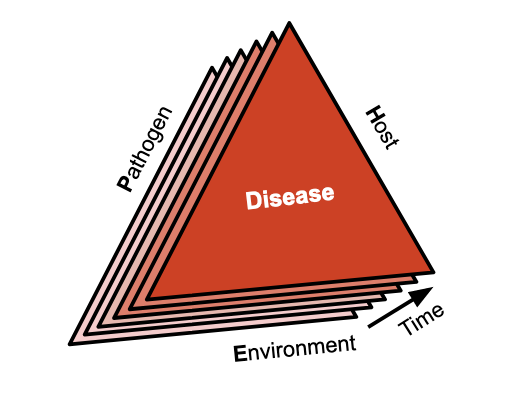
\includegraphics[width=3.92708in,height=\textheight]{imgs/prism.png}

}

\caption{\label{fig-prism}The plant disease prism as a model of plant
disease epidemics}

\end{figure}

\hypertarget{importance-of-epidemics}{%
\section{Importance of epidemics}\label{importance-of-epidemics}}

Epidemics bear significant economic importance due to their potential to
decrease crop yields, diminish product quality, and escalate control
costs, contingent on their intensity level. Numerous historical examples
of widespread epidemics, reaching pandemic levels and resulting in
catastrophic effects on crops, have been documented (Agrios 2005b). The
Irish potato famine of 1845--1847, caused by the late blight pathogen
(\emph{Phytophthora infestans}), is a famous example of a
well-documented pandemic. This disease notably altered the course of
history in Europe and the United States, and was pivotal in the
evolution of the science of plant pathology. During the 1840s, the
pathogen ravaged potato crops, which were a dietary staple for the
Irish. The disease outbreak was triggered by the introduction of a
novel, virulent pathogen population that found suitable environmental
conditions (cool and wet weather) for infection and development within a
dense population of susceptible hosts.

However, there are several reasons why devastating epidemics may
continue to unfold. Recent history has seen severe epidemics reaching
pandemic levels due to the incursion of pathogens into regions where
they had previously been absent (refer to Box 1). Alternatively, new
pathogenic strains might emerge as a result of factors driving genetic
diversity within the local pathogen population. A case in point is the
Ug99 strain of the wheat stem rust, which poses a significant threat to
global wheat production. First identified in Uganda in 1998, an asexual
lineage has propagated through Africa and the Middle East, causing
catastrophic epidemics. Research suggests that Ug99 emerged via somatic
hybridization and nuclear exchange between isolates from different
lineages (Li et al. 2019). Finally, disease emergence or re-emergence
can be influenced by shifts in climatic patterns. For instance, the
Fusarium head blight of wheat caused by the fungus \emph{Fusarium
graminearum}. In Southern Brazil, the increased frequency of severe
epidemics resulting in greater yield loss since the early 1990s has been
linked to alterations in rainfall patterns across decades (Duffeck et
al. 2020).

\begin{tcolorbox}[enhanced jigsaw, titlerule=0mm, rightrule=.15mm, colbacktitle=quarto-callout-note-color!10!white, opacitybacktitle=0.6, toptitle=1mm, leftrule=.75mm, colback=white, colframe=quarto-callout-note-color-frame, bottomrule=.15mm, toprule=.15mm, breakable, bottomtitle=1mm, coltitle=black, title=\textcolor{quarto-callout-note-color}{\faInfo}\hspace{0.5em}{Box 1: Diseases on the move}, arc=.35mm, opacityback=0, left=2mm]

In Brazil, the soybean rust pathogen (\emph{Phakopsora pachyrhizi})
first reached southern Brazil in 2002 (Yorinori et al. 2005). The
disease spread to all production regions of the country in the following
few years, severely reducing yields. To overcome the problem, farmers
have relied on massive applications of fungicides on soybeans, which
dramatically increased the production costs with the need for sequential
fungicide sprays to combat the disease. Total economic loss have been
estimated at around US\$ 2 billion yearly (Godoy et al. 2016). More
recently, wheat blast, a disease that originated in the south of Brazil
in 1984, and have been restricted to South America, was firstly spotted
in South Asia, Bangladesh, in 2016. Blast epidemics in that occasion
devastated more than 15,000 ha of wheat and reduced yield of wheat in
the affected field up to 100\% (Malaker et al. 2016; Islam et al. 2019).
The disease was later found in Zambia, thus also becoming a threat to
wheat production in Africa (Tembo et al. 2020). In Brazil, the wheat
blast disease is a current threat to expansion of wheat cultivation in
the tropics(Cruz and Valent 2017).

\end{tcolorbox}

\hypertarget{history-of-epidemiology}{%
\section{History of Epidemiology}\label{history-of-epidemiology}}

Botanical epidemiology, or the study of plant disease epidemics, is a
discipline with roots tracing back to the early 1960s. However, its
origins can be linked to events from centuries and decades prior. For
instance, in 1728, Duhamel de Monceau presented the earliest known
epidemiological work on a disease, referred to as `Death,' that
afflicted saffron crocus (\emph{Rhizoctonia violacea}). Fast forward to
1858, a textbook detailing plant diseases, written by Julius Kuhn, made
its debut, introducing the concept of an epidemic as illustrated by the
Irish late blight epidemics of 1845-46. Subsequently, in 1901, H.M. Ward
adopted an ecological perspective to the study of plant diseases in his
seminal book, Disease in Plants. By 1946, Gäumann penned the first book
exclusively devoted to plant disease epidemiology.

Further evolution of this field was marked by the publication of a
chapter titled ``Analysis of Epidemics'' by J.E. Vanderplank in Plant
Pathology, vol.~3, edited by Horsfall and Dimond, in 1960. Vanderplank
elaborated on his pioneering ideas in his 1963 book, ``Plant Diseases:
Epidemics and Control''(Vanderplank 1963). He is universally recognized
as the foundational figure of plant disease epidemiology (Zadoks and
Schein 1988; Thresh 1998), his landmark book being the first to
comprehensively describe and quantify plant disease epidemics, and
offering a theoretical framework for epidemic analysis.

In the same year, the first International Epidemiology Workshop was
convened in Pau, France. This event constitutes an important milestone
in the historical narrative, significantly contributing to the molding
of this emergent discipline.

\begin{figure}

{\centering 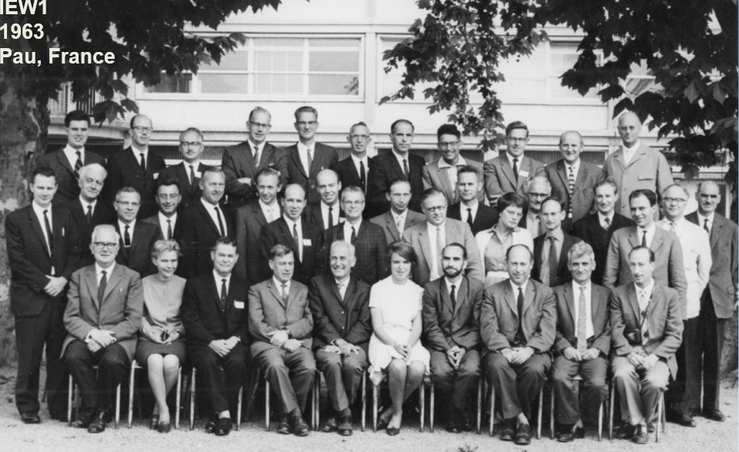
\includegraphics[width=5.38542in,height=\textheight]{imgs/iew1.png}

}

\caption{\label{fig-iew1}Group photo of the First International
Epidemiology Workshop}

\end{figure}

The \textbf{International Epidemiology Workshop (IEW)} is the principal
working group of plant disease epidemiology. This is an organization
with a rich history whose members have met approximately every 5 years
since 1963. Thus far, \href{https://iew13.net/about.html}{13 meetings}
have been organized/planned:

1963 - Pau, France\\
1971 - Wageningen, The Netherlands\\
1979 - Penn State, United States\\
1983 - NC State, Raleigh, United States\\
1986 - Jerusalem, Israel\\
1990 - Giessen, Germany\\
1994 - Papendal, The Netherlands\\
2001 - Ouro Preto, Brazil\\
2005 - Landerneau, France\\
2009 - Cornell, Geneva, United States\\
2013 - Beijing, China\\
2018 - Lillehammer, Norway\\
2024 - Iguassu Falls, Brazil

\hypertarget{other-resources}{%
\section{Other resources}\label{other-resources}}

\hypertarget{books}{%
\subsection{Books}\label{books}}

2006 - \href{https://link.springer.com/book/10.1007/1-4020-4581-6}{The
Epidemiology of Plant Diseases}\\
2007 -
\href{https://apsjournals.apsnet.org/doi/book/10.1094/9780890545058}{The
Study of Plant Disease Epidemics}\\
2017 -
\href{https://apsjournals.apsnet.org/doi/book/10.1094/9780890544426}{Exercises
in Plant Disease Epidemiology}\\
2017 -
\href{https://apsjournals.apsnet.org/doi/book/10.1094/9780890544877}{Application
of Information Theory to Epidemiology}\\
2020 -
\href{https://apsjournals.apsnet.org/doi/book/10.1094/9780890546383}{Emerging
Plant Diseases and Global Security}\\

\hypertarget{online-tutorials}{%
\subsection{Online tutorials}\label{online-tutorials}}

\href{https://www.apsnet.org/edcenter/disimpactmngmnt/topc/EcologyAndEpidemiologyInR/Pages/default.aspx}{Ecology
and Epidemiology in R}\\
\href{https://www.apsnet.org/edcenter/disimpactmngmnt/topc/EpidemiologyTemporal/Pages/default.aspx}{Plant
Disease Epidemiology - Temporal aspects}\\
\href{https://www.apsnet.org/edcenter/disimpactmngmnt/topc/BotanicalEpidemiology/Pages/default.aspx}{Simulation
Modeling in Plant Disease Epidemiology and Crop Loss Analysis}

\hypertarget{software}{%
\subsection{Software}\label{software}}

\href{http://adamhsparks.github.io/epicrop/}{Epicrop - Simulation
Modeling of Crop Diseases using a SEIR model}

\part{Epidemic data}

\hypertarget{disease-variables}{%
\chapter{Disease variables}\label{disease-variables}}

\hypertarget{disease-quantification}{%
\section{Disease quantification}\label{disease-quantification}}

Studies on the temporal progression or spatial spread of epidemics
cannot be conducted without field-collected data, or, in some cases,
simulated data. The study of plant disease quantification, termed
Phytopathometry, is a subdivision of plant pathology concerned with the
science of disease measurement. It has strong ties to the field of
epidemiology (Bock et al. 2021b).

Traditionally, disease quantification has been executed through visual
evaluation. However, the past few decades have witnessed significant
advancements in imaging and remote sensing technologies (which don't
necessitate contact with the object), leaving a profound impact on this
field. As such, disease quantity can now be gauged through estimation
(visually, by the human eye) or measurement (through remote sensing
technologies such as RGB, MSI, and HSI)
Figure~\ref{fig-disease_measure}.

While the utilization of digital or remote sensing technology for
disease measurement or estimation provides a more objective approach,
visual assessment is largely subjective. It is known to vary among human
raters, as these raters differ in their innate abilities, training, and
how they are influenced by the chosen method (e.g., scales). Disease is
estimated or measured on a specimen within a population, or on a sample
of specimens drawn from that population. The specimen in question can be
a plant organ, an individual plant, a group of plants, a field, or a
farm. The specific specimen type also determines the terminology used to
describe disease quantity.

\begin{figure}

{\centering 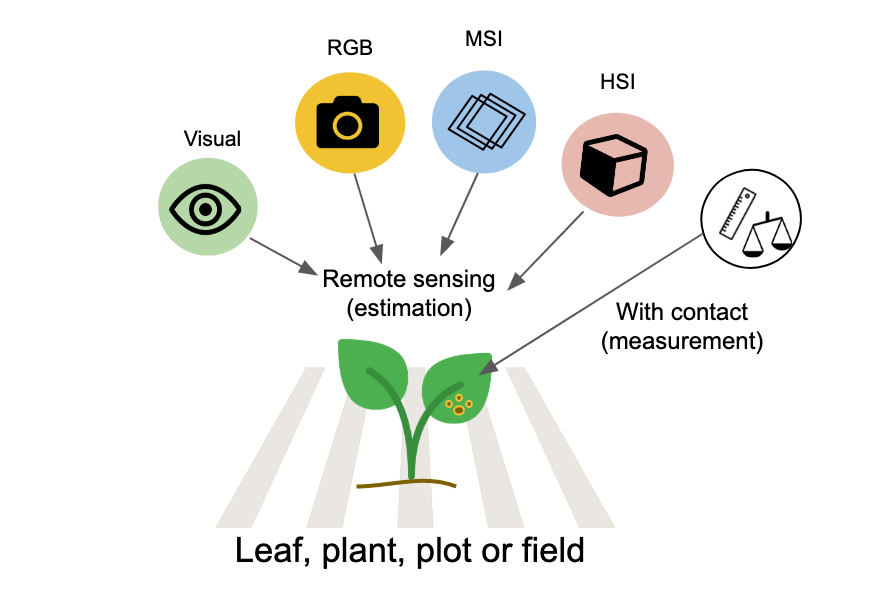
\includegraphics[width=5.10417in,height=\textheight]{imgs/disease_measure.png}

}

\caption{\label{fig-disease_measure}Different approaches used to obtain
estimates or measures of plant disease. RGB = red, green, blue; MSI =
multispectral imaging; HSI = hyperspectral imaging.}

\end{figure}

inally, while developing new or refining existing disease assessment
methods, it is crucial to evaluate the reliability of the assessments
made by different raters or instruments, as well as their
accuracy---specifically, how close the estimations or measurements are
to the reference (or gold standard) values. Several methods are
available for assessing the reliability, precision, and accuracy of
these estimates or measurements (see
\href{data-accuracy.html}{definitions}). The choice of methods depends
on the objective of the work, but largely on the type or nature of the
data. These considerations will be further discussed.

\hypertarget{disease-variables-1}{%
\section{Disease variables}\label{disease-variables-1}}

A common term used to reference the quantity of disease, irrespective of
how it is expressed, is `disease intensity'. This term, however, has
minimal practical value as it only implies that the disease is more or
less ``intense''. We require more specific terminology to standardize
the reference to disease quantity and methodology. One of the primary
tasks in disease assessment is classifying each specimen, often in a
sample or within a population, as diseased or not diseased. This binary
(yes/no or 1/0) evaluation may sufficiently express disease intensity if
the goal is to ascertain the number or proportion of diseased specimens
in a sample or a population.

This discussion brings us to two terms: disease incidence and
prevalence. Incidence is typically used to denote the proportion or
number (count) of plants (or their organs) deemed as observational units
at the field scale or below. On the other hand, prevalence refers to the
proportion or number of fields or farms with diseased plants within a
larger production area or region (Nutter et al. 2006)
Figure~\ref{fig-prevalence_incidence}. Therefore, prevalence is
analogous to incidence, with the only difference being the spatial scale
of the sampling unit.

\begin{figure}

{\centering 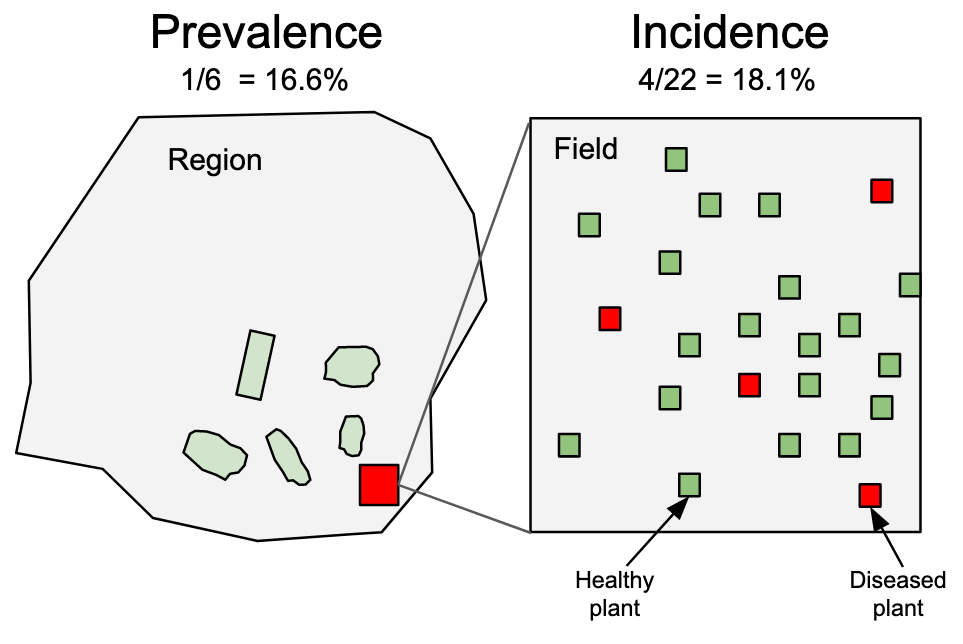
\includegraphics[width=5in,height=\textheight]{imgs/prevalence_incidence.png}

}

\caption{\label{fig-prevalence_incidence}Schematic representation of how
prevalence and incidence of plant diseases are calculated depending on
the spatial scale of the assessment}

\end{figure}

In many instances, it's necessary to determine the degree to which a
specimen is diseased, a concept defined as disease severity. In certain
contexts, severity is narrowly defined as the proportion of the unit
that exhibits symptoms (Nutter et al. 2006). However, a more expansive
view of severity includes additional metrics such as nominal or ordinal
scores, lesion count, and percent area affected (ratio scale). Ordinal
scales are broken down into rank-ordered classes (see specific
\href{data-ordinal.html}{section}), defined based on either a percentage
scale or descriptions of symptoms (Bock et al. 2021b). Occasionally,
disease is expressed in terms of (average) lesion size or area, which
could be regarded as a measure of severity. These variables represent
different levels of measurements that provide varying degrees of
information about the disease quantity - from low (nominal scale) to
high (ratio scale) Figure~\ref{fig-severity}.

\begin{figure}

{\centering 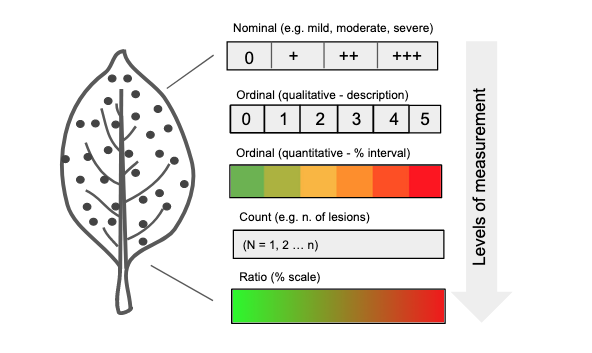
\includegraphics[width=5.32292in,height=\textheight]{imgs/severity.png}

}

\caption{\label{fig-severity}Scales and associated levels of measurement
used to describe severity of plant diseases}

\end{figure}

\hypertarget{data-types}{%
\section{Data types}\label{data-types}}

The data used to express disease as incidence or any form of severity
measurements can be discrete or continuous in nature.

Discrete variables are countable (involving integers) at a particular
point in time. In other words, only a finite number of values (nominal
or ordinal) is possible, and these cannot be subdivided. For instance, a
plant or plant part can be either diseased or not diseased (nominal
data). It's not possible to count 1.5 diseased plants. Furthermore, a
plant classified as diseased may exhibit a certain number of lesions
(count data), or be categorized into a specific severity class (ordinal
data, common in ordinal scales, e.g., 1-9). Disease data in the form of
counts often relates to the number of infections per sampling units.
Most commonly, these counts refer to the assessed pathogen population,
such as the number of airborne or soilborne propagules.

In contrast to discrete variables, continuous variables can be measured
on a scale and can assume any numeric value between two points. For
example, the size of a lesion on a plant can be measured at a very
precise scale (cm or mm). An estimate of severity on a percent scale (\%
diseased area) can take any value between non-zero and 100\%. Although
incidence at the individual level is discrete, at the sample level it
can be treated as continuous, as it can assume any value in proportion
or percentage.

Disease variables can also be characterized by a statistical
distribution, which are models that provide the probability of a
specific value (or a range of values) being drawn from a particular
distribution. Understanding statistical or mathematical distributions is
a crucial step in improving our grasp of data collection methods,
experiment design, and data analysis processes such as data
summarization or hypothesis testing.

\hypertarget{statistical-distributions-and-simulation}{%
\section{Statistical distributions and
simulation}\label{statistical-distributions-and-simulation}}

\hypertarget{binomial-distribution}{%
\subsection{Binomial distribution}\label{binomial-distribution}}

For incidence (and prevalence), the data is binary at the individual
level, as there are only two possible outcomes in a \emph{trial}: the
plant or plant part is disease or not diseased. The statistical
distribution that best describe the incidence data at the individual
level is the \emph{binomial distribution}.

Let's simulate the binomial outcomes for a range of probabilities in a
sample of 100 units, using the \texttt{rbinom()} function in R. For a
single trial (e.g., status of plants in a single plant row), the
\texttt{size} argument is set to 1.

\begin{Shaded}
\begin{Highlighting}[]
\FunctionTok{library}\NormalTok{(tidyverse)}
\FunctionTok{library}\NormalTok{(r4pde)}


\FunctionTok{set.seed}\NormalTok{(}\DecValTok{123}\NormalTok{) }\CommentTok{\# for reproducibility}
\NormalTok{P}\FloatTok{.1} \OtherTok{\textless{}{-}} \FunctionTok{rbinom}\NormalTok{(}\DecValTok{100}\NormalTok{, }\AttributeTok{size =} \DecValTok{1}\NormalTok{, }\AttributeTok{prob =} \FloatTok{0.1}\NormalTok{)}
\NormalTok{P}\FloatTok{.3} \OtherTok{\textless{}{-}} \FunctionTok{rbinom}\NormalTok{(}\DecValTok{100}\NormalTok{, }\AttributeTok{size =} \DecValTok{1}\NormalTok{, }\AttributeTok{prob =} \FloatTok{0.3}\NormalTok{)}
\NormalTok{P}\FloatTok{.7} \OtherTok{\textless{}{-}} \FunctionTok{rbinom}\NormalTok{(}\DecValTok{100}\NormalTok{, }\AttributeTok{size =} \DecValTok{1}\NormalTok{, }\AttributeTok{prob =} \FloatTok{0.7}\NormalTok{)}
\NormalTok{P}\FloatTok{.9} \OtherTok{\textless{}{-}} \FunctionTok{rbinom}\NormalTok{(}\DecValTok{100}\NormalTok{, }\AttributeTok{size =} \DecValTok{1}\NormalTok{, }\AttributeTok{prob =} \FloatTok{0.9}\NormalTok{)}
\NormalTok{binomial\_data }\OtherTok{\textless{}{-}} \FunctionTok{data.frame}\NormalTok{(P}\FloatTok{.1}\NormalTok{, P}\FloatTok{.3}\NormalTok{, P}\FloatTok{.7}\NormalTok{, P}\FloatTok{.9}\NormalTok{)}
\end{Highlighting}
\end{Shaded}

We can then visualize the plots.

\begin{Shaded}
\begin{Highlighting}[]
\NormalTok{binomial\_data }\SpecialCharTok{|\textgreater{}}
  \FunctionTok{pivot\_longer}\NormalTok{(}\DecValTok{1}\SpecialCharTok{:}\DecValTok{4}\NormalTok{, }\AttributeTok{names\_to =} \StringTok{"P"}\NormalTok{,}
               \AttributeTok{values\_to =} \StringTok{"value"}\NormalTok{) }\SpecialCharTok{|\textgreater{}}
  \FunctionTok{ggplot}\NormalTok{(}\FunctionTok{aes}\NormalTok{(value)) }\SpecialCharTok{+}
  \FunctionTok{geom\_histogram}\NormalTok{(}\AttributeTok{fill =} \StringTok{"\#339966"}\NormalTok{,}
                 \AttributeTok{bins =} \DecValTok{10}\NormalTok{) }\SpecialCharTok{+}
  \FunctionTok{facet\_wrap}\NormalTok{( }\SpecialCharTok{\textasciitilde{}}\NormalTok{ P) }\SpecialCharTok{+}
  \FunctionTok{theme\_r4pde}\NormalTok{()}
\end{Highlighting}
\end{Shaded}

\begin{figure}

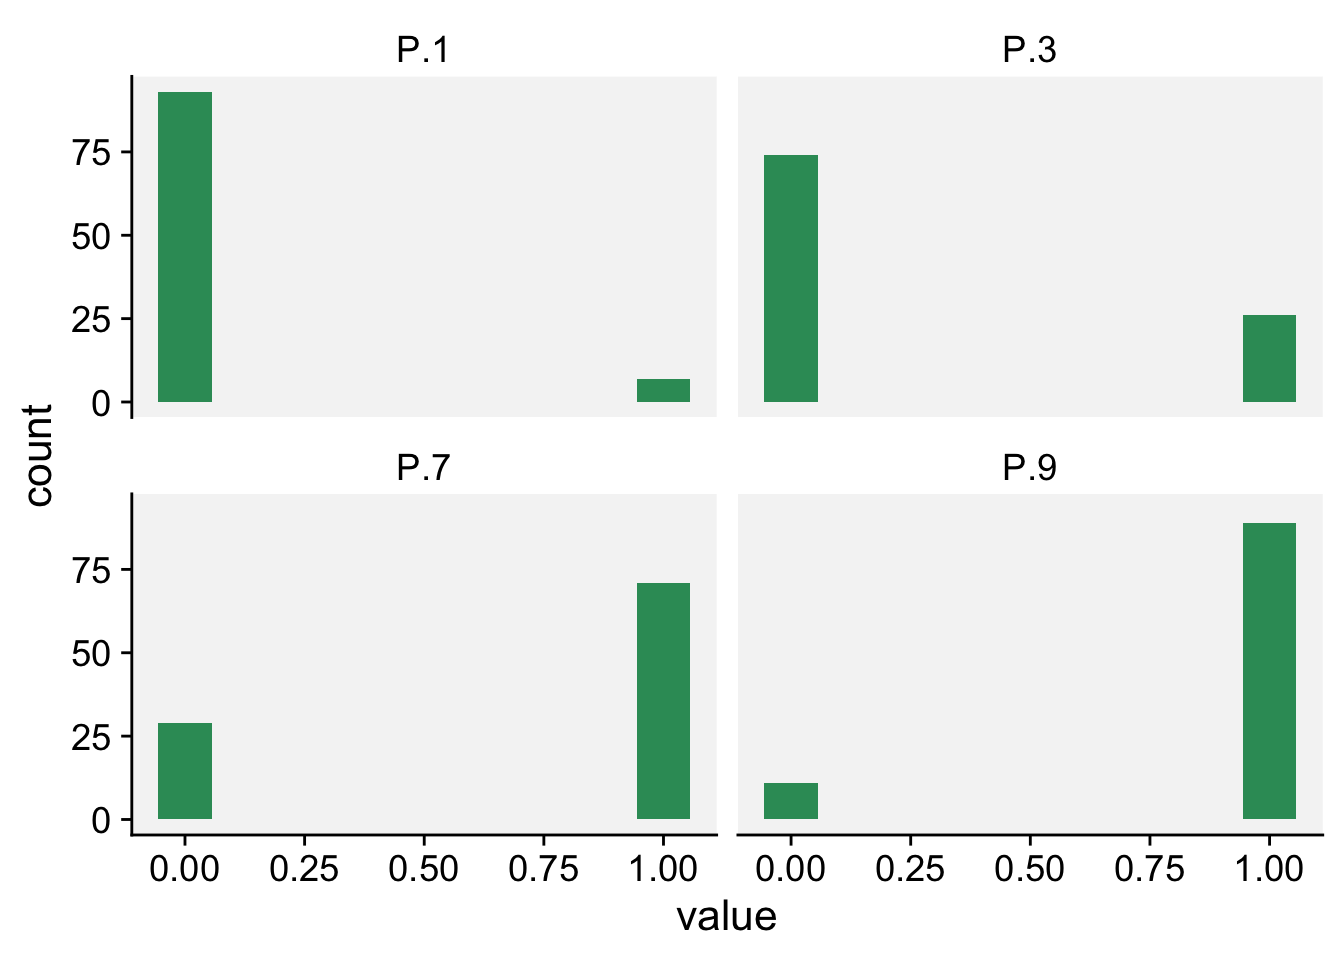
\includegraphics{data-terminology_files/figure-latex/fig-binomial-1.pdf} \hfill{}

\caption{\label{fig-binomial}Binomial distribution to describe binary
data}

\end{figure}

\hypertarget{beta-distribution}{%
\subsection{Beta distribution}\label{beta-distribution}}

In many studies, it's often useful to express these quantities as a
proportion of the total population or sample size, rather than absolute
numbers. This helps standardize the data, making it easier to compare
between different populations or different time periods.

For example, if we're studying a plant disease, we could express disease
incidence as the proportion of plants that are newly diseased during a
given time period. Similarly, disease severity could be expressed as the
proportion of each plant's organ area that is affected by the disease.
These proportions are ratio variables, as they can take on any value
between 0 and 1, and ratios of these variables are meaningful.

The Beta distribution is a probability distribution that is defined
between 0 and 1, which makes it ideal for modeling data that represents
proportions. It's a flexible distribution, as its shape can take many
forms depending on the values of its two parameters, often denoted as
alpha and beta.

Let's simulate some data using the \texttt{rbeta()} function.

\begin{Shaded}
\begin{Highlighting}[]
\NormalTok{beta1}\FloatTok{.5} \OtherTok{\textless{}{-}} \FunctionTok{rbeta}\NormalTok{(}\AttributeTok{n =} \DecValTok{1000}\NormalTok{, }\AttributeTok{shape1 =} \DecValTok{1}\NormalTok{, }\AttributeTok{shape2 =} \DecValTok{5}\NormalTok{)}
\NormalTok{beta5}\FloatTok{.5} \OtherTok{\textless{}{-}} \FunctionTok{rbeta}\NormalTok{(}\AttributeTok{n =} \DecValTok{1000}\NormalTok{, }\AttributeTok{shape1 =} \DecValTok{5}\NormalTok{, }\AttributeTok{shape2 =} \DecValTok{5}\NormalTok{)}
\NormalTok{beta\_data }\OtherTok{\textless{}{-}} \FunctionTok{data.frame}\NormalTok{(beta1}\FloatTok{.5}\NormalTok{, beta5}\FloatTok{.5}\NormalTok{)}
\end{Highlighting}
\end{Shaded}

Notice that there are two shape parameters in the beta distribution:
\texttt{shape1} and \texttt{shape2} to be defined. This makes the
distribution very flexible and with different potential shapes as we can
see below.

\begin{Shaded}
\begin{Highlighting}[]
\NormalTok{beta\_data }\SpecialCharTok{|\textgreater{}}
  \FunctionTok{pivot\_longer}\NormalTok{(}\DecValTok{1}\SpecialCharTok{:}\DecValTok{2}\NormalTok{, }\AttributeTok{names\_to =} \StringTok{"P"}\NormalTok{,}
               \AttributeTok{values\_to =} \StringTok{"value"}\NormalTok{) }\SpecialCharTok{|\textgreater{}}
  \FunctionTok{ggplot}\NormalTok{(}\FunctionTok{aes}\NormalTok{(value)) }\SpecialCharTok{+}
  \FunctionTok{geom\_histogram}\NormalTok{(}\AttributeTok{fill =} \StringTok{"\#339966"}\NormalTok{,}
                 \AttributeTok{color =} \StringTok{"white"}\NormalTok{,}
                 \AttributeTok{bins =} \DecValTok{15}\NormalTok{) }\SpecialCharTok{+}
  \FunctionTok{scale\_x\_continuous}\NormalTok{(}\AttributeTok{limits =} \FunctionTok{c}\NormalTok{(}\DecValTok{0}\NormalTok{, }\DecValTok{1}\NormalTok{)) }\SpecialCharTok{+}
  \FunctionTok{facet\_wrap}\NormalTok{( }\SpecialCharTok{\textasciitilde{}}\NormalTok{ P)}\SpecialCharTok{+}
  \FunctionTok{theme\_r4pde}\NormalTok{()}
\end{Highlighting}
\end{Shaded}

\begin{figure}

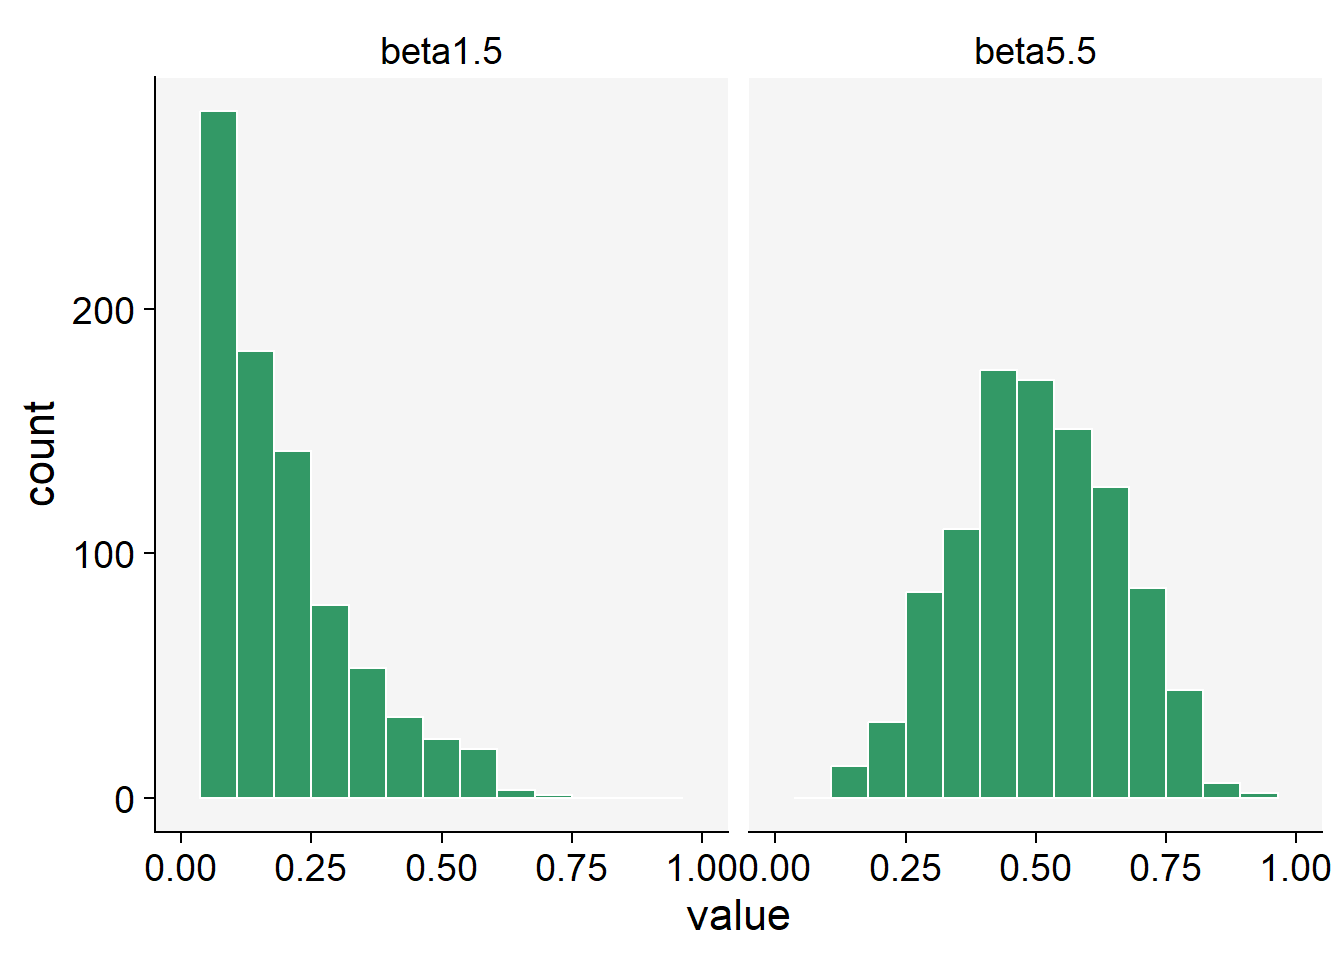
\includegraphics{data-terminology_files/figure-latex/fig-betabin-1.pdf} \hfill{}

\caption{\label{fig-betabin}Binomial distribution to describe proportion
data}

\end{figure}

\hypertarget{beta-binomial-distribution}{%
\subsection{Beta-binomial
distribution}\label{beta-binomial-distribution}}

The Beta-Binomial distribution is a mixture of the Binomial distribution
with the Beta distribution acting as a prior on the probability
parameter of the binomial. Disease probabilities can vary across trials
due to a number of unobserved or unmeasured factors. This variability
can result in overdispersion, a phenomenon where the observed variance
in the data is greater than what the binomial distribution expects.

This is where the Beta-Binomial distribution comes in handy. By
combining the Beta distribution's flexibility in modeling probabilities
with the Binomial distribution's discrete event modeling, it provides an
extra layer of variability to account for overdispersion. The
Beta-Binomial distribution treats the probability of success (disease
occurrence in this context) as a random variable itself, following a
Beta distribution. This means the probability can vary from trial to
trial.

Therefore, when we observe data that shows more variance than the Beta
distribution can account for, or when we believe there are underlying
factors causing variability in the probability of disease occurrence,
the Beta-Binomial distribution is a more appropriate model. It captures
both the variability in success probability as well as the occurrence of
the discrete event (disease incidence).

When combined with the Binomial distribution, which handles discrete
events (e.g.~whether an individual is diseased or not), the
Beta-Binomial distribution allows us to make probabilistic predictions
about these events. For example, based on prior data (the Beta
distribution), we can estimate the likelihood of a particular individual
being diseased (the Binomial distribution).

In R, the \texttt{rBetaBin} function of the \emph{FlexReg} package
generates random values from the beta-binomial distribution. The
arguments of the function are \texttt{n}, or the number of values to
generate; if length(\texttt{n}) \textgreater{} 1, the length is taken to
be the number required. \texttt{size} is he total number of trials.
\texttt{mu} is the mean parameter. It must lie in (0, 1). \texttt{theta}
is the overdispersion parameter. It must lie in (0, 1). \texttt{phi} the
precision parameter. It is an alternative way to specify the theta
parameter. It must be a positive real value.

\begin{Shaded}
\begin{Highlighting}[]
\FunctionTok{library}\NormalTok{(FlexReg) }
\NormalTok{betabin3}\FloatTok{.6} \OtherTok{\textless{}{-}} \FunctionTok{rBetaBin}\NormalTok{(}\AttributeTok{n =} \DecValTok{100}\NormalTok{, }\AttributeTok{size =} \DecValTok{40}\NormalTok{, }\AttributeTok{mu =}\NormalTok{ .}\DecValTok{3}\NormalTok{, }\AttributeTok{theta =}\NormalTok{ .}\DecValTok{6}\NormalTok{)}
\NormalTok{betabin7}\FloatTok{.3} \OtherTok{\textless{}{-}} \FunctionTok{rBetaBin}\NormalTok{(}\AttributeTok{n =} \DecValTok{100}\NormalTok{, }\AttributeTok{size =} \DecValTok{40}\NormalTok{, }\AttributeTok{mu =}\NormalTok{ .}\DecValTok{7}\NormalTok{, }\AttributeTok{theta =}\NormalTok{ .}\DecValTok{3}\NormalTok{)}
\NormalTok{betabin\_data }\OtherTok{\textless{}{-}} \FunctionTok{data.frame}\NormalTok{(betabin3}\FloatTok{.6}\NormalTok{, betabin7}\FloatTok{.3}\NormalTok{)}
\end{Highlighting}
\end{Shaded}

\begin{Shaded}
\begin{Highlighting}[]
\NormalTok{betabin\_data }\SpecialCharTok{|\textgreater{}}
  \FunctionTok{pivot\_longer}\NormalTok{(}\DecValTok{1}\SpecialCharTok{:}\DecValTok{2}\NormalTok{, }\AttributeTok{names\_to =} \StringTok{"P"}\NormalTok{,}
               \AttributeTok{values\_to =} \StringTok{"value"}\NormalTok{) }\SpecialCharTok{|\textgreater{}}
  \FunctionTok{ggplot}\NormalTok{(}\FunctionTok{aes}\NormalTok{(value)) }\SpecialCharTok{+}
  \FunctionTok{geom\_histogram}\NormalTok{(}\AttributeTok{fill =} \StringTok{"\#339966"}\NormalTok{,}
                 \AttributeTok{color =} \StringTok{"white"}\NormalTok{,}
                 \AttributeTok{bins =} \DecValTok{15}\NormalTok{) }\SpecialCharTok{+}
  \FunctionTok{facet\_wrap}\NormalTok{( }\SpecialCharTok{\textasciitilde{}}\NormalTok{ P) }\SpecialCharTok{+}
  \FunctionTok{theme\_r4pde}\NormalTok{()}
\end{Highlighting}
\end{Shaded}

\begin{figure}

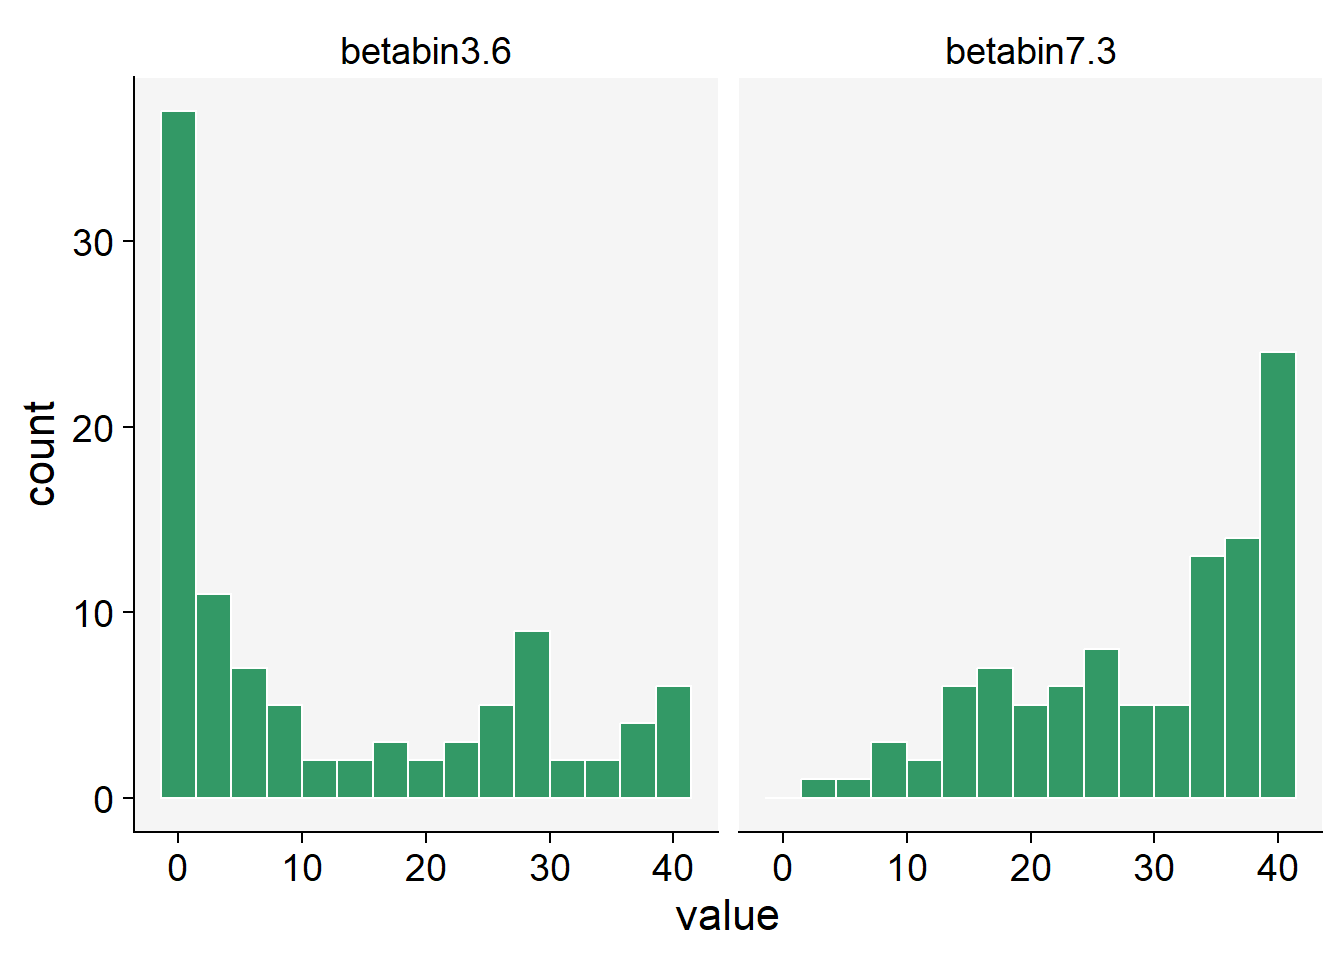
\includegraphics{data-terminology_files/figure-latex/fig-beta-1.pdf} \hfill{}

\caption{\label{fig-beta}Beta-binomial distribution to describe
proportion data}

\end{figure}

\hypertarget{poisson-distribution}{%
\subsection{Poisson distribution}\label{poisson-distribution}}

When conducting studies in epidemiology, specifically plant diseases,
researchers often collect data on the number of diseased plants,
infected plant parts, or individual symptoms, such as lesions. These
variables are counted in whole numbers - 1, 2, 3, etc., making them
discrete variables. Discrete variables contrast with continuous
variables that can take any value within a defined range and can include
fractions or decimals. In addition to being discrete, these variables
are also non-negative, meaning they cannot take negative values. After
all, you can't have a negative number of diseased plants or lesions.
Given these characteristics, a suitable distribution to model such data
is the Poisson distribution. This distribution is particularly suitable
for counting the number of times an event occurs in a given time or
space.

In R, we can used the \texttt{rpois()} function to obtain 100 random
observations following a Poisson distribution. For such, we need to
inform the number of observation (n = 100) and \texttt{lambda}, the
vector of means.

\begin{Shaded}
\begin{Highlighting}[]
\NormalTok{poisson5 }\OtherTok{\textless{}{-}} \FunctionTok{rpois}\NormalTok{(}\DecValTok{100}\NormalTok{, }\AttributeTok{lambda =} \DecValTok{10}\NormalTok{)}
\NormalTok{poisson35 }\OtherTok{\textless{}{-}} \FunctionTok{rpois}\NormalTok{(}\DecValTok{100}\NormalTok{, }\AttributeTok{lambda =} \DecValTok{35}\NormalTok{)}
\NormalTok{poisson\_data }\OtherTok{\textless{}{-}} \FunctionTok{data.frame}\NormalTok{(poisson5, poisson35)}
\end{Highlighting}
\end{Shaded}

\begin{Shaded}
\begin{Highlighting}[]
\NormalTok{poisson\_data }\SpecialCharTok{|\textgreater{}}
  \FunctionTok{pivot\_longer}\NormalTok{(}\DecValTok{1}\SpecialCharTok{:}\DecValTok{2}\NormalTok{, }\AttributeTok{names\_to =} \StringTok{"P"}\NormalTok{,}
               \AttributeTok{values\_to =} \StringTok{"value"}\NormalTok{) }\SpecialCharTok{|\textgreater{}}
  \FunctionTok{ggplot}\NormalTok{(}\FunctionTok{aes}\NormalTok{(value)) }\SpecialCharTok{+}
  \FunctionTok{geom\_histogram}\NormalTok{(}\AttributeTok{fill =} \StringTok{"\#339966"}\NormalTok{,}
                 \AttributeTok{color =} \StringTok{"white"}\NormalTok{,}
                 \AttributeTok{bins =} \DecValTok{15}\NormalTok{) }\SpecialCharTok{+}
  \FunctionTok{facet\_wrap}\NormalTok{( }\SpecialCharTok{\textasciitilde{}}\NormalTok{ P) }\SpecialCharTok{+}
  \FunctionTok{theme\_r4pde}\NormalTok{()}
\end{Highlighting}
\end{Shaded}

\begin{figure}

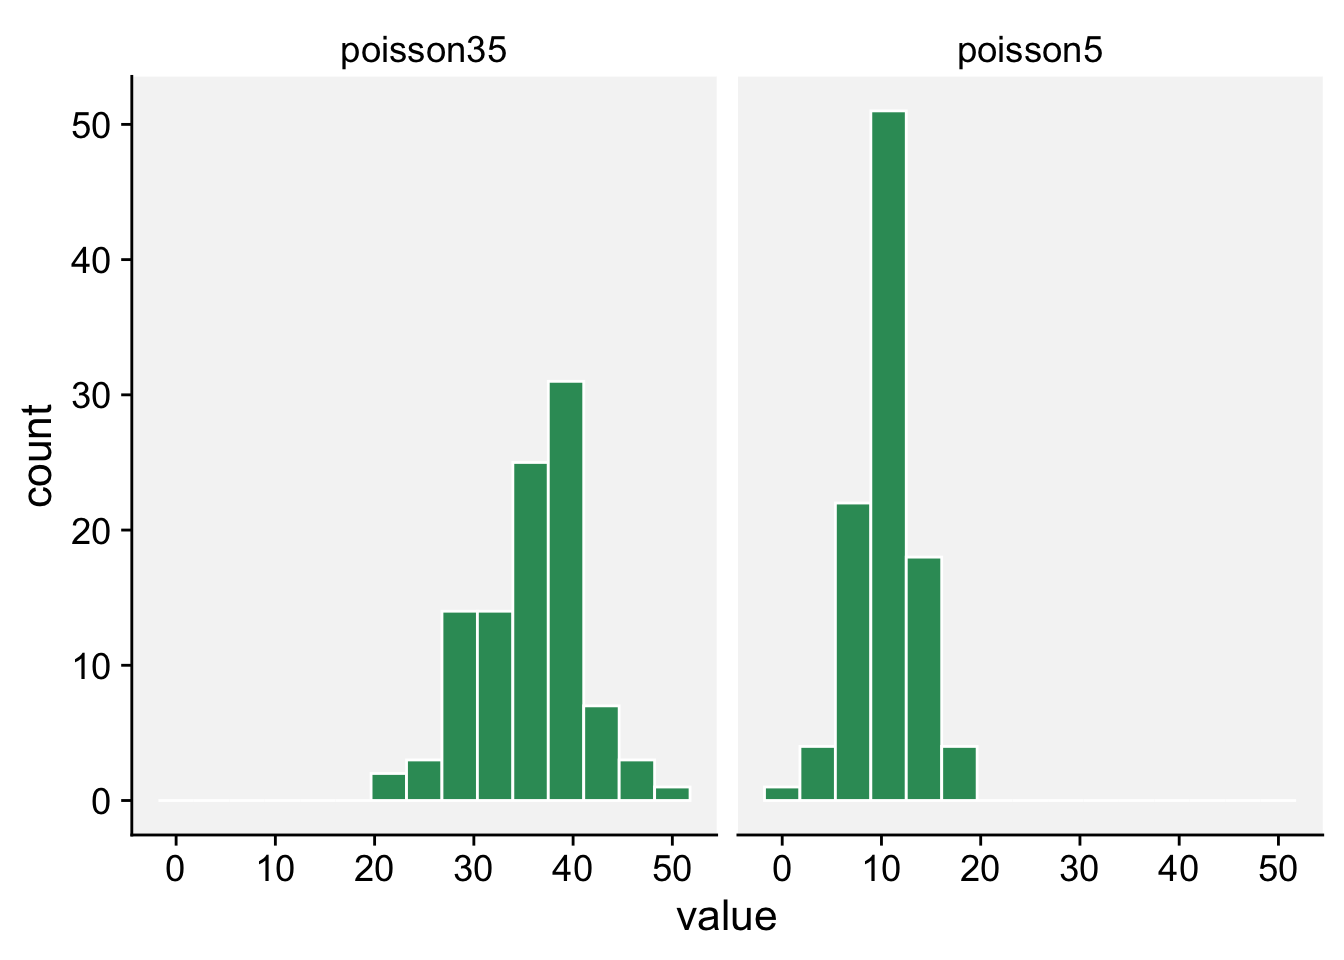
\includegraphics{data-terminology_files/figure-latex/fig-poisson-1.pdf} \hfill{}

\caption{\label{fig-poisson}Poisson distribution to describe count data}

\end{figure}

\hypertarget{negative-binomial-distribution}{%
\subsection{Negative binomial
distribution}\label{negative-binomial-distribution}}

While the Poisson distribution is indeed suitable for modeling count
data, it assumes that the mean and variance of the data are equal.
However, in real-world scenarios, especially in epidemiology, it is
common to encounter overdispersed data - where the variance is greater
than the mean. This could occur, for instance, if there's greater
variability in disease incidence across different plant populations than
would be expected under the Poisson assumption.

In such cases, the Negative Binomial distribution is a better
alternative. The Negative Binomial distribution is a discrete
probability distribution that models the number of successes in a
sequence of independent and identically distributed Bernoulli trials
before a specified (non-random) number of failures occurs.

One of the key features of the Negative Binomial distribution is its
ability to handle overdispersion. Unlike the Poisson distribution, which
has one parameter (lambda, representing the mean and variance), the
Negative Binomial distribution has two parameters. One parameter is the
mean, but the other (often denoted as `size' or `shape') governs the
variance independently, allowing it to be larger than the mean if
necessary. Thus, it provides greater flexibility than the Poisson
distribution for modeling count data and can lead to more accurate
results when overdispersion is present.

In R, we can use the \texttt{rnbinom()} function to generate random
variates from a Negative Binomial distribution. This function requires
the number of observations (\texttt{n}), the target for the number of
successful trials (\texttt{size}), and the probability of each success
(\texttt{prob}).

Here's an example:

\begin{Shaded}
\begin{Highlighting}[]
\CommentTok{\# Generate 100 random variables from a Negative Binomial distribution}
\NormalTok{negbin14}\FloatTok{.6} \OtherTok{\textless{}{-}} \FunctionTok{rnbinom}\NormalTok{(}\AttributeTok{n =} \DecValTok{100}\NormalTok{, }\AttributeTok{size =} \DecValTok{14}\NormalTok{, }\AttributeTok{prob =} \FloatTok{0.6}\NormalTok{)}
\NormalTok{negbin50}\FloatTok{.6} \OtherTok{\textless{}{-}} \FunctionTok{rnbinom}\NormalTok{(}\AttributeTok{n =} \DecValTok{100}\NormalTok{, }\AttributeTok{size =} \DecValTok{50}\NormalTok{, }\AttributeTok{prob =} \FloatTok{0.6}\NormalTok{)}
\NormalTok{negbin\_data }\OtherTok{\textless{}{-}} \FunctionTok{data.frame}\NormalTok{(negbin14}\FloatTok{.6}\NormalTok{, negbin50}\FloatTok{.6}\NormalTok{)}
\end{Highlighting}
\end{Shaded}

\begin{Shaded}
\begin{Highlighting}[]
\NormalTok{negbin\_data }\SpecialCharTok{|\textgreater{}}
  \FunctionTok{pivot\_longer}\NormalTok{(}\DecValTok{1}\SpecialCharTok{:}\DecValTok{2}\NormalTok{, }\AttributeTok{names\_to =} \StringTok{"P"}\NormalTok{,}
               \AttributeTok{values\_to =} \StringTok{"value"}\NormalTok{) }\SpecialCharTok{|\textgreater{}}
  \FunctionTok{ggplot}\NormalTok{(}\FunctionTok{aes}\NormalTok{(value)) }\SpecialCharTok{+}
  \FunctionTok{geom\_histogram}\NormalTok{(}\AttributeTok{fill =} \StringTok{"\#339966"}\NormalTok{,}
                 \AttributeTok{color =} \StringTok{"white"}\NormalTok{, }\AttributeTok{bins =} \DecValTok{15}\NormalTok{) }\SpecialCharTok{+}
  \FunctionTok{facet\_wrap}\NormalTok{( }\SpecialCharTok{\textasciitilde{}}\NormalTok{ P) }\SpecialCharTok{+}
  \FunctionTok{theme\_r4pde}\NormalTok{()}
\end{Highlighting}
\end{Shaded}

\begin{figure}

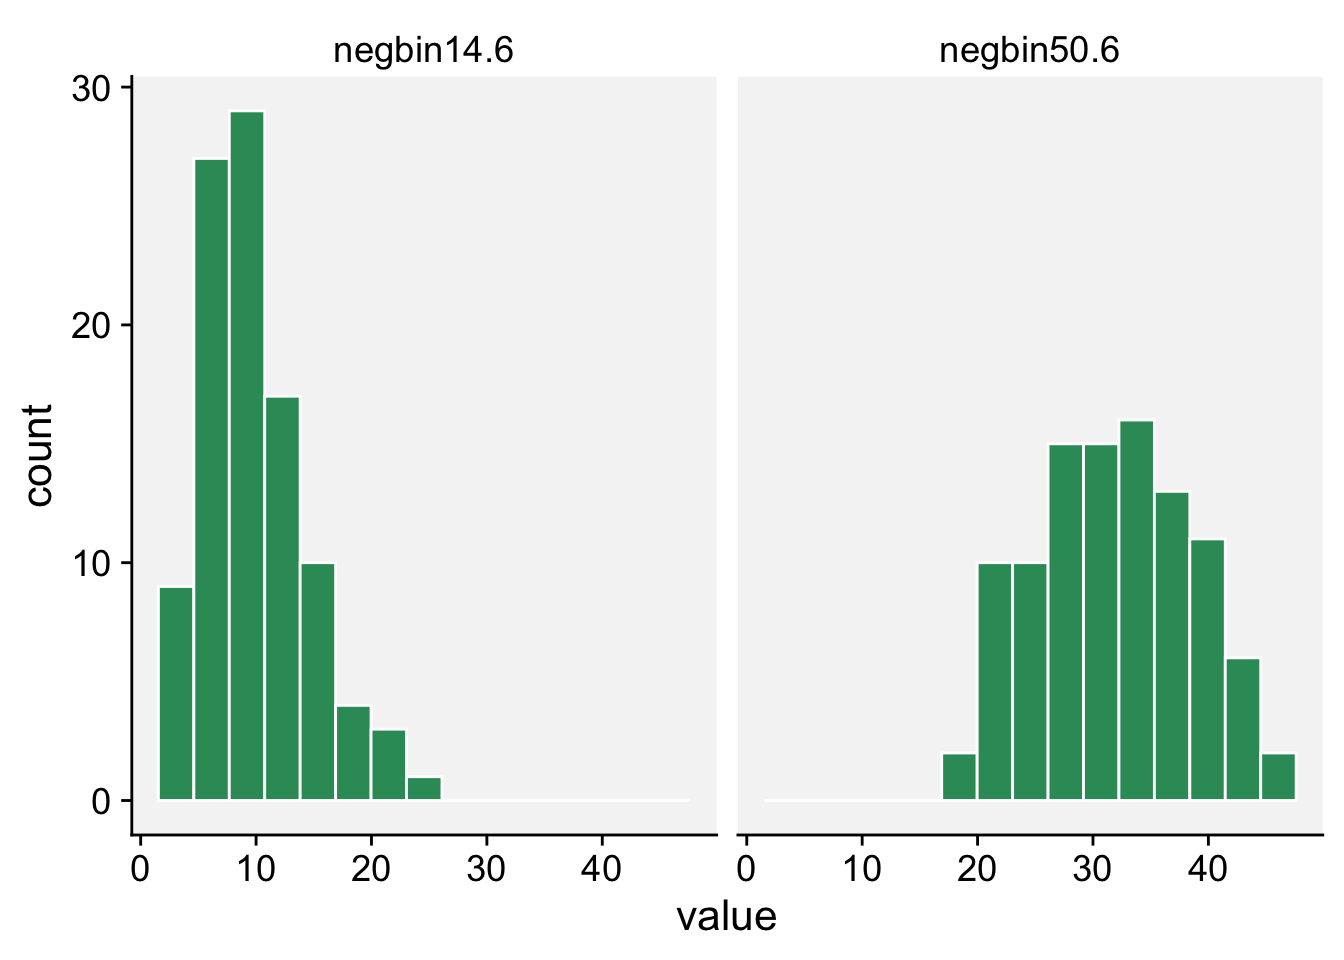
\includegraphics{data-terminology_files/figure-latex/fig-negbin-1.pdf} \hfill{}

\caption{\label{fig-negbin}Negative binomial distribution to describe
overdispersed count data}

\end{figure}

\hypertarget{gamma-distribution}{%
\subsection{Gamma distribution}\label{gamma-distribution}}

In plant disease epidemiology and other fields of study, we may often
encounter continuous variables - these are variables that can take on
any value within a given range, including both whole numbers and
fractions. An example of a continuous variable in this context is lesion
size, which can theoretically be any non-negative value.

Often, researchers use the normal (Gaussian) distribution to model such
continuous variables. The normal distribution is symmetric, bell-shaped,
and is fully described by its mean and standard deviation. However, a
fundamental characteristic of the normal distribution is that it extends
from negative infinity to positive infinity. While this is not a problem
for many applications, it becomes an issue when the variable being
modeled cannot take on negative values - like the size of a lesion.

This is where the Gamma distribution can be a good alternative. The
Gamma distribution is a two-parameter family of continuous probability
distributions, which does not include negative values, making it an
appropriate choice for modeling variables like lesion sizes. While it
might seem a bit more complicated due to its two parameters, this also
allows it a greater flexibility in terms of the variety of shapes and
behaviors it can describe. The Gamma distribution is often used in
various scientific disciplines, including queuing models, climatology,
financial services, and of course, epidemiology. Its main parameters are
the shape and scale (or alternatively shape and rate), which control the
shape, spread and location of the distribution.

We can use the \texttt{rgamma()} function that requires the number of
samples (n = 100 in our case) and the \texttt{shape}, or the mean value.

\begin{Shaded}
\begin{Highlighting}[]
\NormalTok{gamma10 }\OtherTok{\textless{}{-}} \FunctionTok{rgamma}\NormalTok{(}\AttributeTok{n =} \DecValTok{100}\NormalTok{, }\AttributeTok{shape =} \DecValTok{10}\NormalTok{, }\AttributeTok{scale =} \DecValTok{1}\NormalTok{)}
\NormalTok{gamma35 }\OtherTok{\textless{}{-}} \FunctionTok{rgamma}\NormalTok{(}\AttributeTok{n =} \DecValTok{100}\NormalTok{, }\AttributeTok{shape =} \DecValTok{35}\NormalTok{, }\AttributeTok{scale =} \DecValTok{1}\NormalTok{)}
\NormalTok{gamma\_data }\OtherTok{\textless{}{-}} \FunctionTok{data.frame}\NormalTok{(gamma10, gamma35)}
\end{Highlighting}
\end{Shaded}

\begin{Shaded}
\begin{Highlighting}[]
\NormalTok{gamma\_data }\SpecialCharTok{|\textgreater{}}
  \FunctionTok{pivot\_longer}\NormalTok{(}\DecValTok{1}\SpecialCharTok{:}\DecValTok{2}\NormalTok{, }\AttributeTok{names\_to =} \StringTok{"P"}\NormalTok{,}
               \AttributeTok{values\_to =} \StringTok{"value"}\NormalTok{) }\SpecialCharTok{|\textgreater{}}
  \FunctionTok{ggplot}\NormalTok{(}\FunctionTok{aes}\NormalTok{(value)) }\SpecialCharTok{+}
  \FunctionTok{geom\_histogram}\NormalTok{(}\AttributeTok{fill =} \StringTok{"\#339966"}\NormalTok{,}
                 \AttributeTok{color =} \StringTok{"white"}\NormalTok{,}
                 \AttributeTok{bins =} \DecValTok{15}\NormalTok{) }\SpecialCharTok{+}
  \FunctionTok{ylim}\NormalTok{(}\DecValTok{0}\NormalTok{, }\FunctionTok{max}\NormalTok{(gamma\_data}\SpecialCharTok{$}\NormalTok{gamma35)) }\SpecialCharTok{+}
  \FunctionTok{facet\_wrap}\NormalTok{( }\SpecialCharTok{\textasciitilde{}}\NormalTok{ P) }\SpecialCharTok{+}
  \FunctionTok{theme\_r4pde}\NormalTok{()}
\end{Highlighting}
\end{Shaded}

\begin{figure}

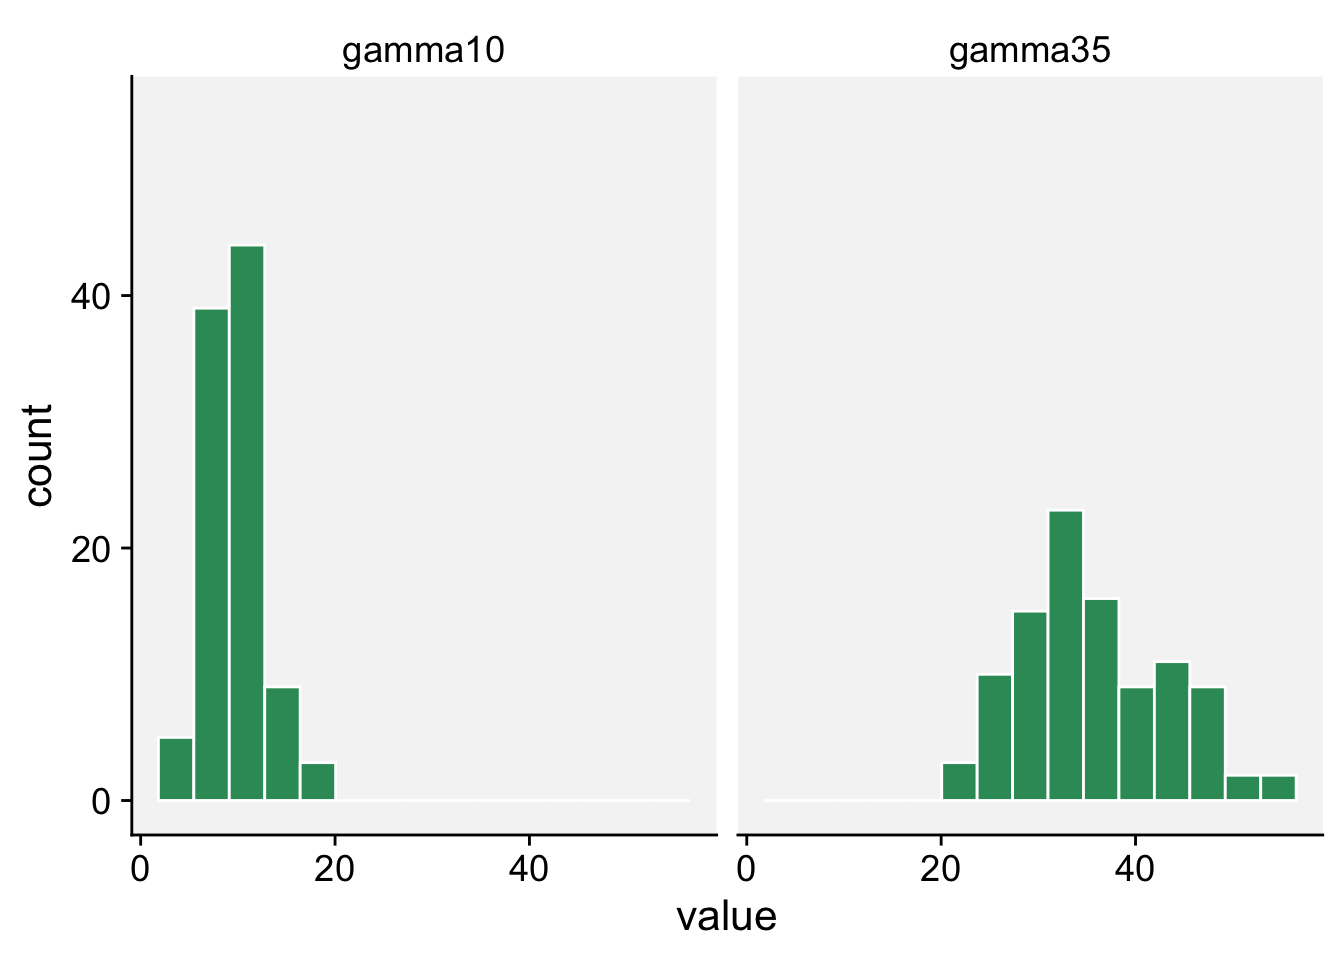
\includegraphics{data-terminology_files/figure-latex/fig-gamma-1.pdf} \hfill{}

\caption{\label{fig-gamma}Gamma distribution to describe continuous
data}

\end{figure}

\hypertarget{simulating-ordinal-data}{%
\subsection{Simulating ordinal data}\label{simulating-ordinal-data}}

Ordinal data is a statistical data type consisting of numerical scores
that fall into a set of categories which are ordered in a meaningful
way. This can include survey responses (e.g., strongly disagree to
strongly agree), levels of achievement (e.g., poor, average, good,
excellent), or, in the case of plant disease, disease severity scales
(e.g., 0 to 5, where 0 represents a healthy plant and 5 represents a
plant with severe symptoms).

When working with ordinal data, we often need to make assumptions about
the distribution of the data. However, unlike continuous data which
might be modeled by a normal or Gamma distribution, or count data which
might be modeled by a Poisson distribution, ordinal data is discrete and
has a clear order but the distances between the categories are not
necessarily equal or known. This makes the modeling process slightly
different.

We can use the \texttt{sample()} function and define the probability
associated with each rank. Let's generate 30 units with a distinct
ordinal score. In the first situation, the higher probabilities (0.5)
are for scores 4 and 5 and lower (0.1) for scores 0 and 1, and in the
second situation is the converse.

\begin{Shaded}
\begin{Highlighting}[]
\NormalTok{ordinal1 }\OtherTok{\textless{}{-}} \FunctionTok{sample}\NormalTok{(}\DecValTok{0}\SpecialCharTok{:}\DecValTok{5}\NormalTok{, }\DecValTok{30}\NormalTok{, }\AttributeTok{replace =} \ConstantTok{TRUE}\NormalTok{, }\AttributeTok{prob =} \FunctionTok{c}\NormalTok{(}\FloatTok{0.1}\NormalTok{, }\FloatTok{0.1}\NormalTok{, }\FloatTok{0.2}\NormalTok{, }\FloatTok{0.2}\NormalTok{, }\FloatTok{0.5}\NormalTok{, }\FloatTok{0.5}\NormalTok{))}
\NormalTok{ordinal2 }\OtherTok{\textless{}{-}} \FunctionTok{sample}\NormalTok{(}\DecValTok{0}\SpecialCharTok{:}\DecValTok{5}\NormalTok{, }\DecValTok{30}\NormalTok{, }\AttributeTok{replace =} \ConstantTok{TRUE}\NormalTok{, }\AttributeTok{prob =} \FunctionTok{c}\NormalTok{(}\FloatTok{0.5}\NormalTok{, }\FloatTok{0.5}\NormalTok{, }\FloatTok{0.2}\NormalTok{, }\FloatTok{0.2}\NormalTok{, }\FloatTok{0.1}\NormalTok{, }\FloatTok{0.1}\NormalTok{))}
\NormalTok{ordinal\_data }\OtherTok{\textless{}{-}} \FunctionTok{data.frame}\NormalTok{(ordinal1, ordinal2)}
\end{Highlighting}
\end{Shaded}

\begin{Shaded}
\begin{Highlighting}[]
\NormalTok{ordinal\_data }\SpecialCharTok{|\textgreater{}}
  \FunctionTok{pivot\_longer}\NormalTok{(}\DecValTok{1}\SpecialCharTok{:}\DecValTok{2}\NormalTok{, }\AttributeTok{names\_to =} \StringTok{"P"}\NormalTok{,}
               \AttributeTok{values\_to =} \StringTok{"value"}\NormalTok{) }\SpecialCharTok{|\textgreater{}}
  \FunctionTok{ggplot}\NormalTok{(}\FunctionTok{aes}\NormalTok{(value)) }\SpecialCharTok{+}
  \FunctionTok{geom\_histogram}\NormalTok{(}\AttributeTok{fill =} \StringTok{"\#339966"}\NormalTok{,}
                 \AttributeTok{color =} \StringTok{"white"}\NormalTok{,}
                 \AttributeTok{bins =} \DecValTok{6}\NormalTok{) }\SpecialCharTok{+}
  \FunctionTok{facet\_wrap}\NormalTok{( }\SpecialCharTok{\textasciitilde{}}\NormalTok{ P) }\SpecialCharTok{+}
  \FunctionTok{theme\_r4pde}\NormalTok{()}
\end{Highlighting}
\end{Shaded}

\begin{figure}

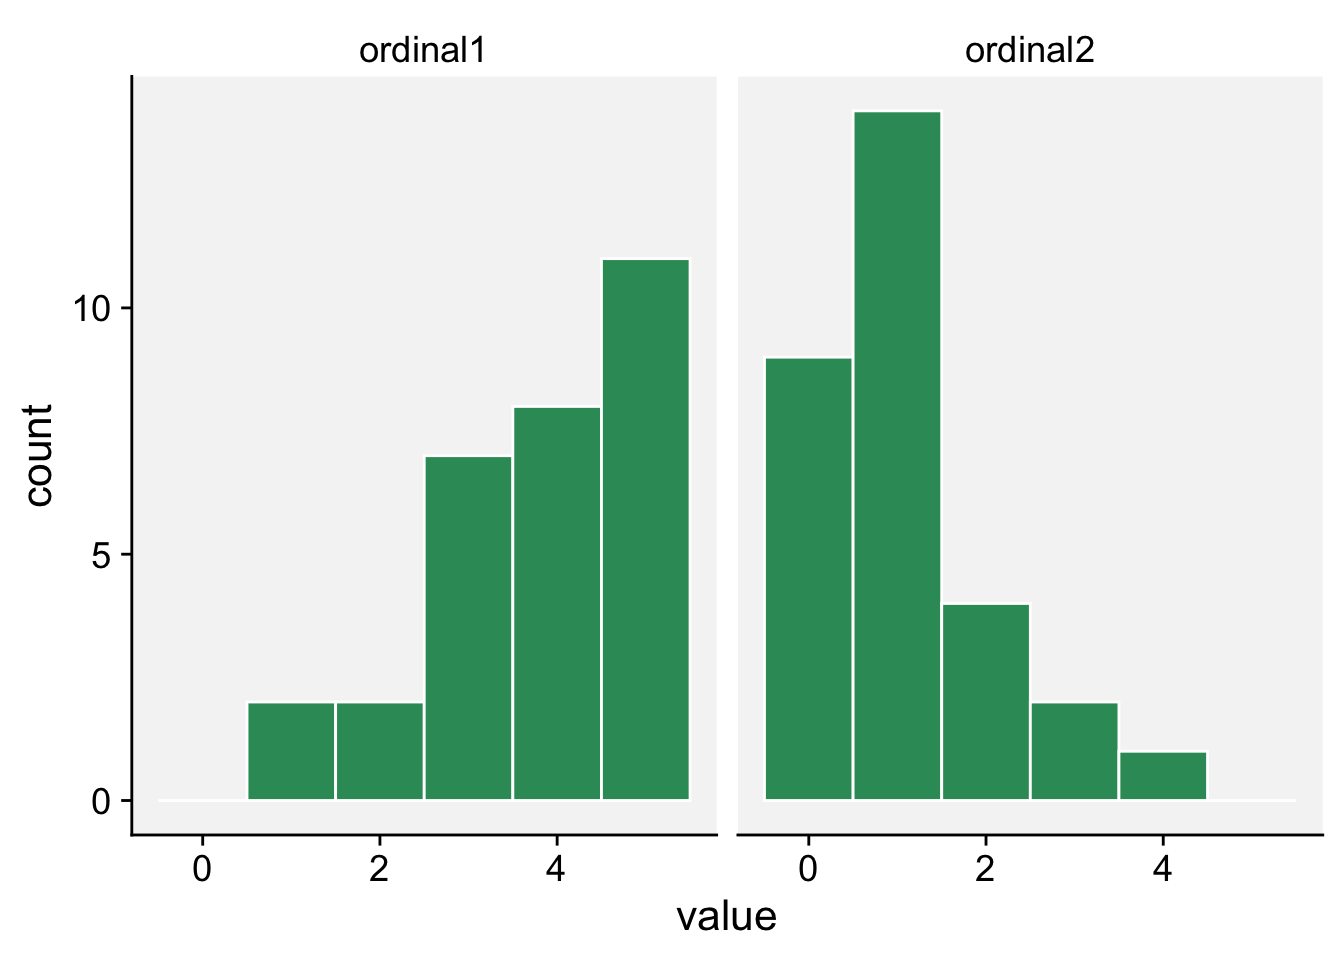
\includegraphics{data-terminology_files/figure-latex/fig-ordinal-1.pdf} \hfill{}

\caption{\label{fig-ordinal}Sampling of ordinal data}

\end{figure}

\hypertarget{ordinal-scales}{%
\chapter{Ordinal scales}\label{ordinal-scales}}

\hypertarget{ordinal-scales-1}{%
\section{Ordinal scales}\label{ordinal-scales-1}}

Ordinal scales are organized as rank-ordered numeric classes, with a
finite number of such classes. The utilization of ordinal scales is
often due to their convenience and speed of rating (Madden et al.
2007d). In plant pathological research, there are two commonly used
types of ordinal scales: quantitative and qualitative (Chiang and Bock
2021).

\hypertarget{quantitative-ordinal}{%
\subsection{Quantitative ordinal}\label{quantitative-ordinal}}

In the quantitative ordinal scale, each score signifies a defined
interval of the percentage scale. The most renowned quantitative ordinal
scale is the Horsfall-Barratt (HB) scale, which was developed in the
early 1940s when the science of plant pathology was transitioning
towards more quantitative methodologies (Hebert 1982). The HB scale
partitions the percentage scale into twelve successive,
logarithmic-based intervals of severity ranging from 0 to 100\%. The
intervals increase in size from 0 to 50\% and decrease from 50 to 100\%.

\begin{tcolorbox}[enhanced jigsaw, titlerule=0mm, rightrule=.15mm, colbacktitle=quarto-callout-warning-color!10!white, opacitybacktitle=0.6, toptitle=1mm, leftrule=.75mm, colback=white, colframe=quarto-callout-warning-color-frame, bottomrule=.15mm, toprule=.15mm, breakable, bottomtitle=1mm, coltitle=black, title=\textcolor{quarto-callout-warning-color}{\faExclamationTriangle}\hspace{0.5em}{Controversy of the H-B scale}, arc=.35mm, opacityback=0, left=2mm]

The divisions of the H-B scale were established on two assumptions. The
first was the logarithmic relationship between the intensity of a
stimulus and the subsequent sensation. The second was the propensity of
a rater to focus on smaller objects when observing objects of two colors
(Madden et al. 2007d). This foundation is based on the so-called
Weber-Fechner law. However, there is limited experimental evidence
supporting these assumptions. Current evidence indicates a linear
relationship, rather than a logarithmic one, between visually estimated
and actual severity (Nutter and Esker 2006). Additionally, these authors
demonstrated that raters more accurately discriminated disease severity
between 25\% and 50\% than what the H-B scale allowed. New scale
structures have been proposed to address the issues associated with the
H-B scale (Liu et al. 2019; Chiang et al. 2014). The Chiang scale
follows a linear relationship with the percentage area diseased at
severities greater than 10\% (class 6 on the scale).

\end{tcolorbox}

Let's input the HB scale data and store as a data frame in R so we can
prepare a table and a plot.

\begin{Shaded}
\begin{Highlighting}[]
\NormalTok{HB }\OtherTok{\textless{}{-}}\NormalTok{ tibble}\SpecialCharTok{::}\FunctionTok{tribble}\NormalTok{(}
  \SpecialCharTok{\textasciitilde{}}\NormalTok{ordinal, }\SpecialCharTok{\textasciitilde{}}\StringTok{\textquotesingle{}range\textquotesingle{}}\NormalTok{, }\SpecialCharTok{\textasciitilde{}}\NormalTok{midpoint,}
  \DecValTok{0}\NormalTok{,          }\StringTok{\textquotesingle{}0\textquotesingle{}}\NormalTok{,    }\DecValTok{0}\NormalTok{,   }
  \DecValTok{1}\NormalTok{,    }\StringTok{\textquotesingle{}0+ to 3\textquotesingle{}}\NormalTok{,  }\FloatTok{1.5}\NormalTok{,   }
  \DecValTok{2}\NormalTok{,    }\StringTok{\textquotesingle{}3+ to 6\textquotesingle{}}\NormalTok{,  }\FloatTok{4.5}\NormalTok{,   }
  \DecValTok{3}\NormalTok{,   }\StringTok{\textquotesingle{}6+ to 12\textquotesingle{}}\NormalTok{,  }\FloatTok{9.0}\NormalTok{,  }
  \DecValTok{4}\NormalTok{,  }\StringTok{\textquotesingle{}12+ to 25\textquotesingle{}}\NormalTok{, }\FloatTok{18.5}\NormalTok{, }
  \DecValTok{5}\NormalTok{,  }\StringTok{\textquotesingle{}25+ to 50\textquotesingle{}}\NormalTok{, }\FloatTok{37.5}\NormalTok{, }
  \DecValTok{6}\NormalTok{,  }\StringTok{\textquotesingle{}50+ to 75\textquotesingle{}}\NormalTok{, }\FloatTok{62.5}\NormalTok{, }
  \DecValTok{7}\NormalTok{,  }\StringTok{\textquotesingle{}75+ to 88\textquotesingle{}}\NormalTok{, }\FloatTok{81.5}\NormalTok{, }
  \DecValTok{8}\NormalTok{,  }\StringTok{\textquotesingle{}88+ to 94\textquotesingle{}}\NormalTok{, }\FloatTok{91.0}\NormalTok{, }
  \DecValTok{9}\NormalTok{,  }\StringTok{\textquotesingle{}94+ to 97\textquotesingle{}}\NormalTok{, }\FloatTok{95.5}\NormalTok{, }
  \DecValTok{10}\NormalTok{,}\StringTok{\textquotesingle{}97+ to 100\textquotesingle{}}\NormalTok{, }\FloatTok{98.5}\NormalTok{,  }
  \DecValTok{11}\NormalTok{,      }\StringTok{\textquotesingle{}100\textquotesingle{}}\NormalTok{,   }\DecValTok{100} 
\NormalTok{  )}
\NormalTok{knitr}\SpecialCharTok{::}\FunctionTok{kable}\NormalTok{(HB, }\AttributeTok{align =} \StringTok{"c"}\NormalTok{)}
\end{Highlighting}
\end{Shaded}

\hypertarget{tbl-HB}{}
\begin{longtable}[]{@{}ccc@{}}
\caption{\label{tbl-HB}The Horsfal-Barrat quantitative ordinal scale
used as a tool for assessing plant disease severity}\tabularnewline
\toprule\noalign{}
ordinal & range & midpoint \\
\midrule\noalign{}
\endfirsthead
\toprule\noalign{}
ordinal & range & midpoint \\
\midrule\noalign{}
\endhead
\bottomrule\noalign{}
\endlastfoot
0 & 0 & 0.0 \\
1 & 0+ to 3 & 1.5 \\
2 & 3+ to 6 & 4.5 \\
3 & 6+ to 12 & 9.0 \\
4 & 12+ to 25 & 18.5 \\
5 & 25+ to 50 & 37.5 \\
6 & 50+ to 75 & 62.5 \\
7 & 75+ to 88 & 81.5 \\
8 & 88+ to 94 & 91.0 \\
9 & 94+ to 97 & 95.5 \\
10 & 97+ to 100 & 98.5 \\
11 & 100 & 100.0 \\
\end{longtable}

Let's visualize the different sizes of the percent interval encompassing
each score.

\begin{Shaded}
\begin{Highlighting}[]
\FunctionTok{library}\NormalTok{(tidyverse)}
\FunctionTok{library}\NormalTok{(r4pde)}
\NormalTok{HB }\SpecialCharTok{|\textgreater{}} 
  \FunctionTok{ggplot}\NormalTok{(}\FunctionTok{aes}\NormalTok{(midpoint, ordinal))}\SpecialCharTok{+}
  \FunctionTok{geom\_point}\NormalTok{(}\AttributeTok{size =}\DecValTok{2}\NormalTok{)}\SpecialCharTok{+}
  \FunctionTok{geom\_line}\NormalTok{()}\SpecialCharTok{+}
  \FunctionTok{scale\_x\_continuous}\NormalTok{(}\AttributeTok{breaks =} \FunctionTok{c}\NormalTok{(}\DecValTok{0}\NormalTok{, }\DecValTok{3}\NormalTok{, }\DecValTok{6}\NormalTok{, }\DecValTok{12}\NormalTok{, }\DecValTok{25}\NormalTok{, }\DecValTok{50}\NormalTok{, }\DecValTok{75}\NormalTok{, }\DecValTok{88}\NormalTok{, }\DecValTok{94}\NormalTok{, }\DecValTok{97}\NormalTok{))}\SpecialCharTok{+}
  \FunctionTok{scale\_y\_continuous}\NormalTok{(}\AttributeTok{breaks =} \FunctionTok{c}\NormalTok{(}\DecValTok{1}\SpecialCharTok{:}\DecValTok{12}\NormalTok{))}\SpecialCharTok{+}
  \FunctionTok{geom\_vline}\NormalTok{(}\FunctionTok{aes}\NormalTok{(}\AttributeTok{xintercept =} \DecValTok{3}\NormalTok{), }\AttributeTok{linetype =} \DecValTok{2}\NormalTok{)}\SpecialCharTok{+}
  \FunctionTok{geom\_vline}\NormalTok{(}\FunctionTok{aes}\NormalTok{(}\AttributeTok{xintercept =} \DecValTok{6}\NormalTok{), }\AttributeTok{linetype =} \DecValTok{2}\NormalTok{)}\SpecialCharTok{+}
  \FunctionTok{geom\_vline}\NormalTok{(}\FunctionTok{aes}\NormalTok{(}\AttributeTok{xintercept =} \DecValTok{12}\NormalTok{), }\AttributeTok{linetype =} \DecValTok{2}\NormalTok{)}\SpecialCharTok{+}
  \FunctionTok{geom\_vline}\NormalTok{(}\FunctionTok{aes}\NormalTok{(}\AttributeTok{xintercept =} \DecValTok{25}\NormalTok{), }\AttributeTok{linetype =} \DecValTok{2}\NormalTok{)}\SpecialCharTok{+}
  \FunctionTok{geom\_vline}\NormalTok{(}\FunctionTok{aes}\NormalTok{(}\AttributeTok{xintercept =} \DecValTok{50}\NormalTok{), }\AttributeTok{linetype =} \DecValTok{2}\NormalTok{)}\SpecialCharTok{+}
  \FunctionTok{geom\_vline}\NormalTok{(}\FunctionTok{aes}\NormalTok{(}\AttributeTok{xintercept =} \DecValTok{75}\NormalTok{), }\AttributeTok{linetype =} \DecValTok{2}\NormalTok{)}\SpecialCharTok{+}
  \FunctionTok{geom\_vline}\NormalTok{(}\FunctionTok{aes}\NormalTok{(}\AttributeTok{xintercept =} \DecValTok{88}\NormalTok{), }\AttributeTok{linetype =} \DecValTok{2}\NormalTok{)}\SpecialCharTok{+}
  \FunctionTok{geom\_vline}\NormalTok{(}\FunctionTok{aes}\NormalTok{(}\AttributeTok{xintercept =} \DecValTok{94}\NormalTok{), }\AttributeTok{linetype =} \DecValTok{2}\NormalTok{)}\SpecialCharTok{+}
  \FunctionTok{geom\_vline}\NormalTok{(}\FunctionTok{aes}\NormalTok{(}\AttributeTok{xintercept =} \DecValTok{97}\NormalTok{), }\AttributeTok{linetype =} \DecValTok{2}\NormalTok{)}\SpecialCharTok{+}
  \FunctionTok{labs}\NormalTok{(}\AttributeTok{x =} \StringTok{"Percent severity"}\NormalTok{, }\AttributeTok{y =} \StringTok{"HB score"}\NormalTok{)}\SpecialCharTok{+}
  \FunctionTok{theme\_r4pde}\NormalTok{()}
\end{Highlighting}
\end{Shaded}

\begin{figure}

\includegraphics{data-ordinal_files/figure-latex/fig-hb-1.pdf} \hfill{}

\caption{\label{fig-hb}Ordinal scores of the Horsfal-Barrat scale}

\end{figure}

We can repeat those procedures to visualize the Chiang scale.

\begin{Shaded}
\begin{Highlighting}[]
\NormalTok{chiang }\OtherTok{\textless{}{-}}\NormalTok{ tibble}\SpecialCharTok{::}\FunctionTok{tribble}\NormalTok{(}
  \SpecialCharTok{\textasciitilde{}}\NormalTok{ordinal, }\SpecialCharTok{\textasciitilde{}}\StringTok{\textquotesingle{}range\textquotesingle{}}\NormalTok{, }\SpecialCharTok{\textasciitilde{}}\NormalTok{midpoint,}
  \DecValTok{0}\NormalTok{,          }\StringTok{\textquotesingle{}0\textquotesingle{}}\NormalTok{,     }\DecValTok{0}\NormalTok{,   }
  \DecValTok{1}\NormalTok{,  }\StringTok{\textquotesingle{}0+ to 0.1\textquotesingle{}}\NormalTok{,  }\FloatTok{0.05}\NormalTok{,   }
  \DecValTok{2}\NormalTok{,}\StringTok{\textquotesingle{}0.1+ to 0.5\textquotesingle{}}\NormalTok{,   }\FloatTok{0.3}\NormalTok{,   }
  \DecValTok{3}\NormalTok{,  }\StringTok{\textquotesingle{}0.5+ to 1\textquotesingle{}}\NormalTok{,  }\FloatTok{0.75}\NormalTok{,  }
  \DecValTok{4}\NormalTok{,    }\StringTok{\textquotesingle{}1+ to 2\textquotesingle{}}\NormalTok{,   }\FloatTok{1.5}\NormalTok{, }
  \DecValTok{5}\NormalTok{,    }\StringTok{\textquotesingle{}2+ to 5\textquotesingle{}}\NormalTok{,     }\DecValTok{3}\NormalTok{, }
  \DecValTok{6}\NormalTok{,   }\StringTok{\textquotesingle{}5+ to 10\textquotesingle{}}\NormalTok{,   }\FloatTok{7.5}\NormalTok{, }
  \DecValTok{7}\NormalTok{,  }\StringTok{\textquotesingle{}10+ to 20\textquotesingle{}}\NormalTok{,    }\DecValTok{15}\NormalTok{, }
  \DecValTok{8}\NormalTok{,  }\StringTok{\textquotesingle{}20+ to 30\textquotesingle{}}\NormalTok{,    }\DecValTok{25}\NormalTok{, }
  \DecValTok{9}\NormalTok{,  }\StringTok{\textquotesingle{}30+ to 40\textquotesingle{}}\NormalTok{,    }\DecValTok{35}\NormalTok{, }
  \DecValTok{10}\NormalTok{, }\StringTok{\textquotesingle{}40+ to 50\textquotesingle{}}\NormalTok{,    }\DecValTok{45}\NormalTok{,  }
  \DecValTok{11}\NormalTok{, }\StringTok{\textquotesingle{}50+ to 60\textquotesingle{}}\NormalTok{,    }\DecValTok{55}\NormalTok{,}
  \DecValTok{12}\NormalTok{, }\StringTok{\textquotesingle{}60+ to 70\textquotesingle{}}\NormalTok{,    }\DecValTok{65}\NormalTok{,}
  \DecValTok{13}\NormalTok{, }\StringTok{\textquotesingle{}70+ to 80\textquotesingle{}}\NormalTok{,    }\DecValTok{75}\NormalTok{,}
  \DecValTok{14}\NormalTok{, }\StringTok{\textquotesingle{}80+ to 90\textquotesingle{}}\NormalTok{,    }\DecValTok{85}\NormalTok{,}
  \DecValTok{15}\NormalTok{,}\StringTok{\textquotesingle{}90+ to 100\textquotesingle{}}\NormalTok{,   }\DecValTok{95}
\NormalTok{  )}
\NormalTok{knitr}\SpecialCharTok{::}\FunctionTok{kable}\NormalTok{(chiang, }\AttributeTok{align =} \StringTok{"c"}\NormalTok{)}
\end{Highlighting}
\end{Shaded}

\hypertarget{tbl-chiang}{}
\begin{longtable}[]{@{}ccc@{}}
\caption{\label{tbl-chiang}The Chiang quantitative ordinal scale used as
a tool for assessing plant disease severity}\tabularnewline
\toprule\noalign{}
ordinal & range & midpoint \\
\midrule\noalign{}
\endfirsthead
\toprule\noalign{}
ordinal & range & midpoint \\
\midrule\noalign{}
\endhead
\bottomrule\noalign{}
\endlastfoot
0 & 0 & 0.00 \\
1 & 0+ to 0.1 & 0.05 \\
2 & 0.1+ to 0.5 & 0.30 \\
3 & 0.5+ to 1 & 0.75 \\
4 & 1+ to 2 & 1.50 \\
5 & 2+ to 5 & 3.00 \\
6 & 5+ to 10 & 7.50 \\
7 & 10+ to 20 & 15.00 \\
8 & 20+ to 30 & 25.00 \\
9 & 30+ to 40 & 35.00 \\
10 & 40+ to 50 & 45.00 \\
11 & 50+ to 60 & 55.00 \\
12 & 60+ to 70 & 65.00 \\
13 & 70+ to 80 & 75.00 \\
14 & 80+ to 90 & 85.00 \\
15 & 90+ to 100 & 95.00 \\
\end{longtable}

\begin{Shaded}
\begin{Highlighting}[]
\NormalTok{chiang }\SpecialCharTok{|\textgreater{}} 
  \FunctionTok{ggplot}\NormalTok{(}\FunctionTok{aes}\NormalTok{(midpoint, ordinal))}\SpecialCharTok{+}
  \FunctionTok{geom\_point}\NormalTok{(}\AttributeTok{size =}\DecValTok{2}\NormalTok{)}\SpecialCharTok{+}
  \FunctionTok{geom\_line}\NormalTok{()}\SpecialCharTok{+}
  \FunctionTok{scale\_y\_continuous}\NormalTok{(}\AttributeTok{breaks =} \FunctionTok{c}\NormalTok{(}\DecValTok{0}\SpecialCharTok{:}\DecValTok{15}\NormalTok{))}\SpecialCharTok{+}
  \FunctionTok{scale\_x\_continuous}\NormalTok{(}\AttributeTok{breaks =} \FunctionTok{c}\NormalTok{(}\DecValTok{0}\NormalTok{, }\DecValTok{5}\NormalTok{, }\DecValTok{10}\NormalTok{, }\DecValTok{20}\NormalTok{, }\DecValTok{30}\NormalTok{, }\DecValTok{40}\NormalTok{, }\DecValTok{50}\NormalTok{, }\DecValTok{60}\NormalTok{, }\DecValTok{70}\NormalTok{, }\DecValTok{80}\NormalTok{, }\DecValTok{90}\NormalTok{, }\DecValTok{100}\NormalTok{))}\SpecialCharTok{+}
  \FunctionTok{geom\_vline}\NormalTok{(}\FunctionTok{aes}\NormalTok{(}\AttributeTok{xintercept =} \DecValTok{0}\NormalTok{), }\AttributeTok{linetype =} \DecValTok{2}\NormalTok{)}\SpecialCharTok{+}
  \FunctionTok{geom\_vline}\NormalTok{(}\FunctionTok{aes}\NormalTok{(}\AttributeTok{xintercept =} \FloatTok{0.1}\NormalTok{), }\AttributeTok{linetype =} \DecValTok{2}\NormalTok{)}\SpecialCharTok{+}
  \FunctionTok{geom\_vline}\NormalTok{(}\FunctionTok{aes}\NormalTok{(}\AttributeTok{xintercept =} \FloatTok{0.5}\NormalTok{), }\AttributeTok{linetype =} \DecValTok{2}\NormalTok{)}\SpecialCharTok{+}
  \FunctionTok{geom\_vline}\NormalTok{(}\FunctionTok{aes}\NormalTok{(}\AttributeTok{xintercept =} \DecValTok{1}\NormalTok{), }\AttributeTok{linetype =} \DecValTok{2}\NormalTok{)}\SpecialCharTok{+}
  \FunctionTok{geom\_vline}\NormalTok{(}\FunctionTok{aes}\NormalTok{(}\AttributeTok{xintercept =} \DecValTok{2}\NormalTok{), }\AttributeTok{linetype =} \DecValTok{2}\NormalTok{)}\SpecialCharTok{+}
  \FunctionTok{geom\_vline}\NormalTok{(}\FunctionTok{aes}\NormalTok{(}\AttributeTok{xintercept =} \DecValTok{5}\NormalTok{), }\AttributeTok{linetype =} \DecValTok{2}\NormalTok{)}\SpecialCharTok{+}
  \FunctionTok{geom\_vline}\NormalTok{(}\FunctionTok{aes}\NormalTok{(}\AttributeTok{xintercept =} \DecValTok{10}\NormalTok{), }\AttributeTok{linetype =} \DecValTok{2}\NormalTok{)}\SpecialCharTok{+}
  \FunctionTok{geom\_vline}\NormalTok{(}\FunctionTok{aes}\NormalTok{(}\AttributeTok{xintercept =} \DecValTok{20}\NormalTok{), }\AttributeTok{linetype =} \DecValTok{2}\NormalTok{)}\SpecialCharTok{+}
  \FunctionTok{geom\_vline}\NormalTok{(}\FunctionTok{aes}\NormalTok{(}\AttributeTok{xintercept =} \DecValTok{30}\NormalTok{), }\AttributeTok{linetype =} \DecValTok{2}\NormalTok{)}\SpecialCharTok{+}
   \FunctionTok{geom\_vline}\NormalTok{(}\FunctionTok{aes}\NormalTok{(}\AttributeTok{xintercept =} \DecValTok{40}\NormalTok{), }\AttributeTok{linetype =} \DecValTok{2}\NormalTok{)}\SpecialCharTok{+}
   \FunctionTok{geom\_vline}\NormalTok{(}\FunctionTok{aes}\NormalTok{(}\AttributeTok{xintercept =} \DecValTok{50}\NormalTok{), }\AttributeTok{linetype =} \DecValTok{2}\NormalTok{)}\SpecialCharTok{+}
   \FunctionTok{geom\_vline}\NormalTok{(}\FunctionTok{aes}\NormalTok{(}\AttributeTok{xintercept =} \DecValTok{60}\NormalTok{), }\AttributeTok{linetype =} \DecValTok{2}\NormalTok{)}\SpecialCharTok{+}
   \FunctionTok{geom\_vline}\NormalTok{(}\FunctionTok{aes}\NormalTok{(}\AttributeTok{xintercept =} \DecValTok{70}\NormalTok{), }\AttributeTok{linetype =} \DecValTok{2}\NormalTok{)}\SpecialCharTok{+}
   \FunctionTok{geom\_vline}\NormalTok{(}\FunctionTok{aes}\NormalTok{(}\AttributeTok{xintercept =} \DecValTok{80}\NormalTok{), }\AttributeTok{linetype =} \DecValTok{2}\NormalTok{)}\SpecialCharTok{+}
   \FunctionTok{geom\_vline}\NormalTok{(}\FunctionTok{aes}\NormalTok{(}\AttributeTok{xintercept =} \DecValTok{90}\NormalTok{), }\AttributeTok{linetype =} \DecValTok{2}\NormalTok{)}\SpecialCharTok{+}
   \FunctionTok{geom\_vline}\NormalTok{(}\FunctionTok{aes}\NormalTok{(}\AttributeTok{xintercept =} \DecValTok{100}\NormalTok{), }\AttributeTok{linetype =} \DecValTok{2}\NormalTok{)}\SpecialCharTok{+}
  \FunctionTok{labs}\NormalTok{(}\AttributeTok{x =} \StringTok{"Percent severity"}\NormalTok{, }\AttributeTok{y =} \StringTok{"Chiang score"}\NormalTok{)}\SpecialCharTok{+}
  \FunctionTok{theme\_r4pde}\NormalTok{()}
\end{Highlighting}
\end{Shaded}

\begin{figure}

\includegraphics{data-ordinal_files/figure-latex/fig-chiagn-1.pdf} \hfill{}

\caption{\label{fig-chiagn}Ordinal scores of the Chiang scale}

\end{figure}

\hypertarget{qualitative-ordinal}{%
\subsection{Qualitative ordinal}\label{qualitative-ordinal}}

In the qualitative ordinal scale, each class provides a description of
the symptoms. An example is the ordinal 0-3 scale for rating eyespot of
wheat developed by (Scott and Hollins 1974).

\begin{longtable}[]{@{}
  >{\raggedright\arraybackslash}p{(\columnwidth - 2\tabcolsep) * \real{0.3239}}
  >{\raggedright\arraybackslash}p{(\columnwidth - 2\tabcolsep) * \real{0.6761}}@{}}
\caption{Ordinal scale for rating eyespot of wheat (Scott and Hollins
1974)}\tabularnewline
\toprule\noalign{}
\begin{minipage}[b]{\linewidth}\raggedright
Class
\end{minipage} & \begin{minipage}[b]{\linewidth}\raggedright
Description
\end{minipage} \\
\midrule\noalign{}
\endfirsthead
\toprule\noalign{}
\begin{minipage}[b]{\linewidth}\raggedright
Class
\end{minipage} & \begin{minipage}[b]{\linewidth}\raggedright
Description
\end{minipage} \\
\midrule\noalign{}
\endhead
\bottomrule\noalign{}
\endlastfoot
0 & uninfected \\
1 & slight eyespot (or or more small lesion occupying in total less than
half of the circumference of the stem) \\
2 & moderate eyespot (one or more lesions occupying at least half the
circumference of the stem) \\
3 & severe eyespot (stem completely girdled by lesions; tissue softened
so that lodging would really occur) \\
\end{longtable}

\hypertarget{disease-severity-index-dsi}{%
\section{Disease severity index
(DSI)}\label{disease-severity-index-dsi}}

Usually, when quantitative or qualitative ordinal scales are used, the
scores are transformed into an index on a percentage basis, such as the
disease severity index (DSI) which is used in data analysis. The DSI is
a single number that summarizes a large amount of information on disease
severity (Chester 1950). The formula for a DSI (\%) can be written as
follows:

\(DSI = \frac{∑(class \ freq. \ ✕ \ score \  of \ class)} {total \ n \ ✕ \ maximal \ class} ✕ 100\)

The \texttt{DSI()} and \texttt{DSI2()} are part of the \emph{r4pde}
package. Let's see how each function works.

The \texttt{DSI()} allows to automate the calculation of the disease
severity index (DSI) in a series of units (e.g.~leaves) that are further
classified according to ordinal scores. The function requires three
arguments:

\begin{itemize}
\item
  unit = the vector of the number of each unit
\item
  class = the vector of the scores for the units
\item
  max = the maximum value of the scale
\end{itemize}

Let's create a toy data set composed of 12 units where each received an
ordinal score. The vectors were arranged as a data frame named scores.

\begin{Shaded}
\begin{Highlighting}[]
\NormalTok{unit }\OtherTok{\textless{}{-}} \FunctionTok{c}\NormalTok{(}\DecValTok{1}\SpecialCharTok{:}\DecValTok{12}\NormalTok{)}
\NormalTok{class }\OtherTok{\textless{}{-}} \FunctionTok{c}\NormalTok{(}\DecValTok{2}\NormalTok{,}\DecValTok{3}\NormalTok{,}\DecValTok{1}\NormalTok{,}\DecValTok{1}\NormalTok{,}\DecValTok{3}\NormalTok{,}\DecValTok{4}\NormalTok{,}\DecValTok{5}\NormalTok{,}\DecValTok{0}\NormalTok{,}\DecValTok{2}\NormalTok{,}\DecValTok{5}\NormalTok{,}\DecValTok{2}\NormalTok{,}\DecValTok{1}\NormalTok{)}
\NormalTok{ratings }\OtherTok{\textless{}{-}} \FunctionTok{data.frame}\NormalTok{(unit, class)}
\NormalTok{knitr}\SpecialCharTok{::}\FunctionTok{kable}\NormalTok{(ratings)}
\end{Highlighting}
\end{Shaded}

\begin{longtable}[]{@{}rr@{}}
\toprule\noalign{}
unit & class \\
\midrule\noalign{}
\endhead
\bottomrule\noalign{}
\endlastfoot
1 & 2 \\
2 & 3 \\
3 & 1 \\
4 & 1 \\
5 & 3 \\
6 & 4 \\
7 & 5 \\
8 & 0 \\
9 & 2 \\
10 & 5 \\
11 & 2 \\
12 & 1 \\
\end{longtable}

The ordinal score used in this example has 6 as the maximum score. The
function returns the DSI value.

\begin{Shaded}
\begin{Highlighting}[]
\FunctionTok{library}\NormalTok{(r4pde)}
\FunctionTok{DSI}\NormalTok{(ratings}\SpecialCharTok{$}\NormalTok{unit, ratings}\SpecialCharTok{$}\NormalTok{class, }\DecValTok{6}\NormalTok{)}
\end{Highlighting}
\end{Shaded}

\begin{verbatim}
[1] 40.27778
\end{verbatim}

Let's now deal with a situation of multiple plots (five replicates)
where a fixed number of 12 samples were taken and assessed using an
ordinal score. Let's input the data using the \texttt{tribble()}
function. Note that the data is in the wide format.

\begin{Shaded}
\begin{Highlighting}[]
\NormalTok{exp }\OtherTok{\textless{}{-}}\NormalTok{ tibble}\SpecialCharTok{::}\FunctionTok{tribble}\NormalTok{(}
  \SpecialCharTok{\textasciitilde{}}\NormalTok{rep, }\SpecialCharTok{\textasciitilde{}}\StringTok{\textasciigrave{}}\AttributeTok{1}\StringTok{\textasciigrave{}}\NormalTok{, }\SpecialCharTok{\textasciitilde{}}\StringTok{\textasciigrave{}}\AttributeTok{2}\StringTok{\textasciigrave{}}\NormalTok{, }\SpecialCharTok{\textasciitilde{}}\StringTok{\textasciigrave{}}\AttributeTok{3}\StringTok{\textasciigrave{}}\NormalTok{, }\SpecialCharTok{\textasciitilde{}}\StringTok{\textasciigrave{}}\AttributeTok{4}\StringTok{\textasciigrave{}}\NormalTok{, }\SpecialCharTok{\textasciitilde{}}\StringTok{\textasciigrave{}}\AttributeTok{5}\StringTok{\textasciigrave{}}\NormalTok{, }\SpecialCharTok{\textasciitilde{}}\StringTok{\textasciigrave{}}\AttributeTok{6}\StringTok{\textasciigrave{}}\NormalTok{, }\SpecialCharTok{\textasciitilde{}}\StringTok{\textasciigrave{}}\AttributeTok{7}\StringTok{\textasciigrave{}}\NormalTok{, }\SpecialCharTok{\textasciitilde{}}\StringTok{\textasciigrave{}}\AttributeTok{8}\StringTok{\textasciigrave{}}\NormalTok{, }\SpecialCharTok{\textasciitilde{}}\StringTok{\textasciigrave{}}\AttributeTok{9}\StringTok{\textasciigrave{}}\NormalTok{, }\SpecialCharTok{\textasciitilde{}}\StringTok{\textasciigrave{}}\AttributeTok{10}\StringTok{\textasciigrave{}}\NormalTok{, }\SpecialCharTok{\textasciitilde{}}\StringTok{\textasciigrave{}}\AttributeTok{11}\StringTok{\textasciigrave{}}\NormalTok{,}\SpecialCharTok{\textasciitilde{}}\StringTok{\textasciigrave{}}\AttributeTok{12}\StringTok{\textasciigrave{}}\NormalTok{,}
  \DecValTok{1}\NormalTok{, }\DecValTok{2}\NormalTok{, }\DecValTok{3}\NormalTok{, }\DecValTok{1}\NormalTok{, }\DecValTok{1}\NormalTok{, }\DecValTok{3}\NormalTok{, }\DecValTok{4}\NormalTok{, }\DecValTok{5}\NormalTok{, }\DecValTok{0}\NormalTok{, }\DecValTok{2}\NormalTok{, }\DecValTok{5}\NormalTok{, }\DecValTok{2}\NormalTok{, }\DecValTok{1}\NormalTok{,}
  \DecValTok{2}\NormalTok{, }\DecValTok{3}\NormalTok{, }\DecValTok{4}\NormalTok{, }\DecValTok{4}\NormalTok{, }\DecValTok{6}\NormalTok{, }\DecValTok{5}\NormalTok{, }\DecValTok{4}\NormalTok{, }\DecValTok{4}\NormalTok{, }\DecValTok{0}\NormalTok{, }\DecValTok{2}\NormalTok{, }\DecValTok{1}\NormalTok{, }\DecValTok{1}\NormalTok{, }\DecValTok{5}\NormalTok{,}
  \DecValTok{3}\NormalTok{, }\DecValTok{5}\NormalTok{, }\DecValTok{6}\NormalTok{, }\DecValTok{6}\NormalTok{, }\DecValTok{5}\NormalTok{, }\DecValTok{4}\NormalTok{, }\DecValTok{2}\NormalTok{, }\DecValTok{0}\NormalTok{, }\DecValTok{0}\NormalTok{, }\DecValTok{0}\NormalTok{, }\DecValTok{0}\NormalTok{, }\DecValTok{2}\NormalTok{, }\DecValTok{0}\NormalTok{,}
  \DecValTok{4}\NormalTok{, }\DecValTok{5}\NormalTok{, }\DecValTok{6}\NormalTok{, }\DecValTok{0}\NormalTok{, }\DecValTok{0}\NormalTok{, }\DecValTok{0}\NormalTok{, }\DecValTok{3}\NormalTok{, }\DecValTok{3}\NormalTok{, }\DecValTok{2}\NormalTok{, }\DecValTok{1}\NormalTok{, }\DecValTok{0}\NormalTok{, }\DecValTok{2}\NormalTok{, }\DecValTok{3}\NormalTok{, }
  \DecValTok{5}\NormalTok{, }\DecValTok{0}\NormalTok{, }\DecValTok{0}\NormalTok{, }\DecValTok{0}\NormalTok{, }\DecValTok{0}\NormalTok{, }\DecValTok{2}\NormalTok{, }\DecValTok{3}\NormalTok{, }\DecValTok{2}\NormalTok{, }\DecValTok{5}\NormalTok{, }\DecValTok{6}\NormalTok{, }\DecValTok{2}\NormalTok{, }\DecValTok{1}\NormalTok{, }\DecValTok{0}\NormalTok{,}
\NormalTok{)}
\NormalTok{knitr}\SpecialCharTok{::}\FunctionTok{kable}\NormalTok{(exp)}
\end{Highlighting}
\end{Shaded}

\begin{longtable}[]{@{}rrrrrrrrrrrrr@{}}
\toprule\noalign{}
rep & 1 & 2 & 3 & 4 & 5 & 6 & 7 & 8 & 9 & 10 & 11 & 12 \\
\midrule\noalign{}
\endhead
\bottomrule\noalign{}
\endlastfoot
1 & 2 & 3 & 1 & 1 & 3 & 4 & 5 & 0 & 2 & 5 & 2 & 1 \\
2 & 3 & 4 & 4 & 6 & 5 & 4 & 4 & 0 & 2 & 1 & 1 & 5 \\
3 & 5 & 6 & 6 & 5 & 4 & 2 & 0 & 0 & 0 & 0 & 2 & 0 \\
4 & 5 & 6 & 0 & 0 & 0 & 3 & 3 & 2 & 1 & 0 & 2 & 3 \\
5 & 0 & 0 & 0 & 0 & 2 & 3 & 2 & 5 & 6 & 2 & 1 & 0 \\
\end{longtable}

After reshaping the data to the long format, we can calculate the DSI
for each plot/replicate as follows:

\begin{Shaded}
\begin{Highlighting}[]
\NormalTok{res }\OtherTok{\textless{}{-}}\NormalTok{ exp }\SpecialCharTok{|\textgreater{}} 
  \FunctionTok{pivot\_longer}\NormalTok{(}\DecValTok{2}\SpecialCharTok{:}\DecValTok{13}\NormalTok{, }\AttributeTok{names\_to =} \StringTok{"unit"}\NormalTok{, }\AttributeTok{values\_to =} \StringTok{"class"}\NormalTok{) }\SpecialCharTok{|\textgreater{}}
  \FunctionTok{group\_by}\NormalTok{(rep) }\SpecialCharTok{|\textgreater{}} 
  \FunctionTok{summarise}\NormalTok{(}\AttributeTok{DSI =} \FunctionTok{DSI}\NormalTok{(unit, class, }\DecValTok{6}\NormalTok{))}
\end{Highlighting}
\end{Shaded}

And here we have the results of the DSI for each replicate.

\begin{Shaded}
\begin{Highlighting}[]
\NormalTok{knitr}\SpecialCharTok{::}\FunctionTok{kable}\NormalTok{(res, }\AttributeTok{align =} \StringTok{"c"}\NormalTok{)}
\end{Highlighting}
\end{Shaded}

\begin{longtable}[]{@{}cc@{}}
\toprule\noalign{}
rep & DSI \\
\midrule\noalign{}
\endhead
\bottomrule\noalign{}
\endlastfoot
1 & 40.27778 \\
2 & 54.16667 \\
3 & 41.66667 \\
4 & 34.72222 \\
5 & 29.16667 \\
\end{longtable}

Now our data set is organized as the frequency of each class as follows:

\begin{Shaded}
\begin{Highlighting}[]
\NormalTok{ratings2 }\OtherTok{\textless{}{-}}\NormalTok{ ratings }\SpecialCharTok{|\textgreater{}} 
\NormalTok{  dplyr}\SpecialCharTok{::}\FunctionTok{count}\NormalTok{(class)}

\NormalTok{ratings2}
\end{Highlighting}
\end{Shaded}

\begin{verbatim}
  class n
1     0 1
2     1 3
3     2 3
4     3 2
5     4 1
6     5 2
\end{verbatim}

Now we can apply the \texttt{DSI2()} function. The function requires
three arguments:

\begin{itemize}
\tightlist
\item
  class = the number of the respective class
\item
  freq = the frequency of the class
\item
  max = the maximum value of the scale
\end{itemize}

\begin{Shaded}
\begin{Highlighting}[]
\FunctionTok{library}\NormalTok{(r4pde)}
\FunctionTok{DSI2}\NormalTok{(ratings2}\SpecialCharTok{$}\NormalTok{class, ratings2}\SpecialCharTok{$}\NormalTok{n, }\DecValTok{6}\NormalTok{)}
\end{Highlighting}
\end{Shaded}

\begin{verbatim}
[1] 40.27778
\end{verbatim}

\hypertarget{image-analysis}{%
\chapter{Image analysis}\label{image-analysis}}

\hypertarget{the-actual-severity-measure}{%
\section{The actual severity
measure}\label{the-actual-severity-measure}}

Among the various methods to express plant disease severity, the percent
area affected (or symptomatic) by the disease is one of the most common,
especially when dealing with diseases that affect leaves. In order to
evaluate whether visual estimates of plant disease severity are
sufficiently accurate (as discussed in the previous chapter), we require
the actual severity values. These are also essential when creating
Standard Area Diagrams (SADs), which are diagrammatic representations of
severity values used as a reference either before or during visual
assessment to standardize and produce more accurate results across
different raters (Del Ponte et al. 2017).

The actual severity values are typically approximated using image
analysis, wherein the image is segmented, and each pixel is categorized
into one of three classes:

\begin{enumerate}
\def\labelenumi{\arabic{enumi}.}
\tightlist
\item
  Diseased (or symptomatic)
\item
  Non-diseased (or healthy)
\item
  Background (the non-plant portion of the image)
\end{enumerate}

The ratio of the diseased area to the total area of the unit (e.g., the
entire plant organ or section of the image) yields the proportion of the
diseased area, or the percent area affected (when multiplied by 100).
Researchers have employed various proprietary or open-source software to
determine the actual severity, as documented in a review on Standard
Area Diagrams (Del Ponte et al. 2017).

In this section, we will utilize the \texttt{measure\_disease()}
function from the \{pliman\} (Plant IMage ANalysis) R package (Olivoto
2022), and its variations, to measure the percent area affected. The
package was compared with other software for determining plant disease
severity across five different plant diseases and was shown to produce
accurate results in most cases (Olivoto et al. 2022).

There are essentially two methods to measure severity. The first is
predicated on image palettes that define each class of the image. The
second relies on RGB-based indices (Alves et al. 2021). Let's explore
the first method, as well as an interactive approach to setting color
palettes.

\hypertarget{image-palettes}{%
\section{Image palettes}\label{image-palettes}}

The most crucial step is the initial one, where the user needs to
correctly define the color palettes for each class. In pliman, the
palettes can be separate images representing each of the three classes:
background (b), symptomatic (s), and healthy (h).

The reference image palettes can be constructed by manually sampling
small areas of the image and creating a composite image. As expected,
the results may vary depending on how these areas are selected. A study
that validated pliman for determining disease severity demonstrated the
effect of different palettes prepared independently by three
researchers, in which the composite palette (combining the three users)
was superior (Olivoto et al. 2022). During the calibration of the
palettes, examining the processed masks is crucial to create reference
palettes that are the most representative of the respective class.

In this example, I manually selected and pasted several sections of
images representing each class from a few leaves into a Google slide.
Once the image palette was ready, I exported each one as a separate PNG
image file (JPG also works). These files were named: sbr\_b.png,
sbr\_h.png, and sbr\_s.png. They can be found
\href{https://github.com/emdelponte/epidemiology-R/tree/main/imgs}{here
in this folder} for downloading.

\begin{figure}

{\centering 

\href{Fig_palettes}{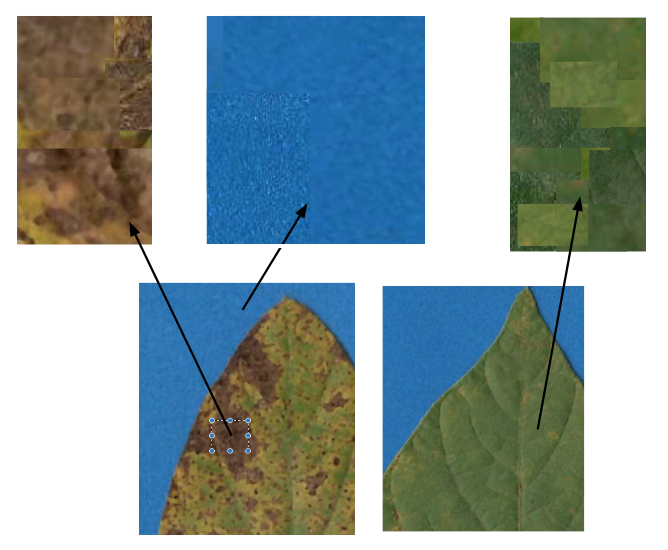
\includegraphics{imgs/pliman1.png}}

}

\caption{\label{fig-pliman1}Preparation of image palettes by manually
sampling fraction of the images that represent background, heatlhy leaf
and lesions}

\end{figure}

Now that we have the image palettes, we need to import them into the
environment, using \texttt{image\_import()} function for further
analysis. Let's create an image object for each palette named h
(healthy), s (symptoms) and b (background).

\begin{Shaded}
\begin{Highlighting}[]
\FunctionTok{library}\NormalTok{(pliman)}
\NormalTok{h }\OtherTok{\textless{}{-}} \FunctionTok{image\_import}\NormalTok{(}\StringTok{"imgs/sbr\_h.png"}\NormalTok{)}
\NormalTok{s }\OtherTok{\textless{}{-}} \FunctionTok{image\_import}\NormalTok{(}\StringTok{"imgs/sbr\_s.png"}\NormalTok{)}
\NormalTok{b }\OtherTok{\textless{}{-}} \FunctionTok{image\_import}\NormalTok{(}\StringTok{"imgs/sbr\_b.png"}\NormalTok{)}
\end{Highlighting}
\end{Shaded}

We can visualize the imported image palettes using the
\texttt{image\_combine()} function.

\begin{Shaded}
\begin{Highlighting}[]
\FunctionTok{image\_combine}\NormalTok{(h, s, b, }\AttributeTok{ncol =}\DecValTok{3}\NormalTok{)}
\end{Highlighting}
\end{Shaded}

\begin{figure}

\includegraphics{data-actual-severity_files/figure-latex/fig-palettes-1.pdf} \hfill{}

\caption{\label{fig-palettes}Image palettes created to segment images
into background, sypomtoms and healthy area of the image}

\end{figure}

An alternative way to set the palettes is to use the
\texttt{pick\_palette()} function. It allows to manually pick the colors
for each class by clicking on top of the imported image. We can use one
of the original images or a composite images with portions of several
leaves. Let's use here one of the original images and pick the
background colors and assigned to \texttt{b} vector.

\begin{Shaded}
\begin{Highlighting}[]
\NormalTok{img }\OtherTok{\textless{}{-}} \FunctionTok{image\_import}\NormalTok{(}\StringTok{"imgs/originals/img5.png"}\NormalTok{)}
\NormalTok{b }\OtherTok{\textless{}{-}} \FunctionTok{pick\_palette}\NormalTok{(img)}
\end{Highlighting}
\end{Shaded}

The original image is displayed and the user needs to click on the
background colors to select the pixels. A message will be displayed as
follows:

\begin{quote}
Use the first mouse button to pick up points in the plot. Press Esc to
exit.
\end{quote}

\begin{figure}

{\centering 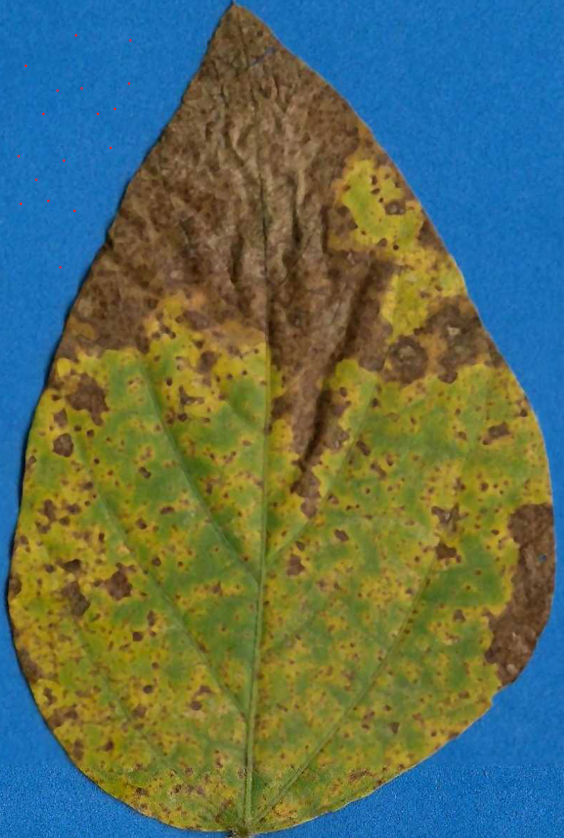
\includegraphics[width=3.53125in,height=\textheight]{imgs/sbr_pick_palette.png}

}

\caption{Soybean rust leaf with small red dots at the upper leaf portion
that indicate which colors were selected for the background}

\end{figure}

After pressing ESC, the image palette for the background is constructed
and can be displayed.

\begin{Shaded}
\begin{Highlighting}[]
\FunctionTok{image\_combine}\NormalTok{(b)}
\end{Highlighting}
\end{Shaded}

\begin{figure}

{\centering 
\includegraphics[width=3.875in,height=\textheight]{imgs/b_picked.png}

}

\caption{Image generating after picking the palette colors for the
background of the leaf}

\end{figure}

Now, we can proceed and pick the colors for the other categories
following the same logic.

\begin{Shaded}
\begin{Highlighting}[]
\CommentTok{\# Symptoms}
\NormalTok{s }\OtherTok{\textless{}{-}} \FunctionTok{pick\_palette}\NormalTok{(img)}

\CommentTok{\# healthy}
\NormalTok{h }\OtherTok{\textless{}{-}} \FunctionTok{pick\_palette}\NormalTok{(img)}
\end{Highlighting}
\end{Shaded}

\hypertarget{measuring-severity}{%
\section{Measuring severity}\label{measuring-severity}}

\hypertarget{single-image}{%
\subsection{Single image}\label{single-image}}

\hypertarget{using-color-palettes}{%
\subsubsection{Using color palettes}\label{using-color-palettes}}

To determine severity in a single image (e.g.~img46.png), the image file
needs to be loaded and assigned to an object using the same
\texttt{image\_import()} function used to load the palettes. We can then
visualize the image, again using \texttt{image\_combine()}.

\begin{tcolorbox}[enhanced jigsaw, titlerule=0mm, rightrule=.15mm, colbacktitle=quarto-callout-tip-color!10!white, opacitybacktitle=0.6, toptitle=1mm, leftrule=.75mm, colback=white, colframe=quarto-callout-tip-color-frame, bottomrule=.15mm, toprule=.15mm, breakable, bottomtitle=1mm, coltitle=black, title=\textcolor{quarto-callout-tip-color}{\faLightbulb}\hspace{0.5em}{Tip}, arc=.35mm, opacityback=0, left=2mm]

The collection of images used in this chapter can be found
\href{https://github.com/emdelponte/epidemiology-R/tree/main/imgs/originals}{here}.

\end{tcolorbox}

\begin{Shaded}
\begin{Highlighting}[]
\NormalTok{img }\OtherTok{\textless{}{-}} \FunctionTok{image\_import}\NormalTok{(}\StringTok{"imgs/originals/img46.png"}\NormalTok{)}
\FunctionTok{image\_combine}\NormalTok{(img)}
\end{Highlighting}
\end{Shaded}

\begin{figure}

\includegraphics{data-actual-severity_files/figure-latex/fig-img-1.pdf} \hfill{}

\caption{\label{fig-img}Imported image for further analysis}

\end{figure}

Now the engaging part starts with the \texttt{measure\_disease()}
function. Four arguments are required when using the reference image
palettes: the image representing the target image and the three images
of the color palettes. As the author of the package states, ``pliman
will take care of all the details!'' The severity is the value displayed
under `symptomatic' in the output.

\begin{Shaded}
\begin{Highlighting}[]
\FunctionTok{set.seed}\NormalTok{(}\DecValTok{123}\NormalTok{)}
\FunctionTok{measure\_disease}\NormalTok{(}
  \AttributeTok{img =}\NormalTok{ img,}
  \AttributeTok{img\_healthy =}\NormalTok{ h,}
  \AttributeTok{img\_symptoms =}\NormalTok{ s,}
  \AttributeTok{img\_background =}\NormalTok{ b}
\NormalTok{)}
\end{Highlighting}
\end{Shaded}

\includegraphics{data-actual-severity_files/figure-latex/unnamed-chunk-7-1.pdf}

If we want to show the mask with two colors instead of the original, we
can set to FALSE two ``show\_'' arguments:

\begin{Shaded}
\begin{Highlighting}[]
\FunctionTok{set.seed}\NormalTok{(}\DecValTok{123}\NormalTok{)}
\FunctionTok{measure\_disease}\NormalTok{(}
  \AttributeTok{img =}\NormalTok{ img,}
  \AttributeTok{img\_healthy =}\NormalTok{ h,}
  \AttributeTok{img\_symptoms =}\NormalTok{ s,}
  \AttributeTok{img\_background =}\NormalTok{ b,}
  \AttributeTok{show\_contour =} \ConstantTok{FALSE}\NormalTok{,}
  \AttributeTok{show\_original =} \ConstantTok{FALSE}
\NormalTok{)}
\end{Highlighting}
\end{Shaded}

\includegraphics{data-actual-severity_files/figure-latex/unnamed-chunk-8-1.pdf}

\hypertarget{multiple-images}{%
\subsection{Multiple images}\label{multiple-images}}

Measuring severity in single images is indeed engaging, but we often
deal with multiple images, not just one. Using the above procedure to
process each image individually would be time-consuming and potentially
tedious.

To automate the process, \{pliman\} offers a batch processing approach.
Instead of using the \texttt{img} argument, one can use the
\texttt{pattern} argument and define the prefix of the image names.
Moreover, we also need to specify the directory where the original files
are located.

If the user wants to save the processed masks, they should set the
\texttt{save\_image} argument to TRUE and also specify the directory
where the images will be saved. Here's an example of how to process 10
images of soybean rust symptoms. The output is a \texttt{list} object
with the measures of the percent healthy and percent symptomatic area
for each leaf in the \texttt{severity} object.

\begin{Shaded}
\begin{Highlighting}[]
\NormalTok{pliman }\OtherTok{\textless{}{-}} \FunctionTok{measure\_disease}\NormalTok{(}
  \AttributeTok{pattern =} \StringTok{"img"}\NormalTok{,}
  \AttributeTok{dir\_original =} \StringTok{"imgs/originals"}\NormalTok{ ,}
  \AttributeTok{dir\_processed =} \StringTok{"imgs/processed"}\NormalTok{,}
  \AttributeTok{save\_image =} \ConstantTok{TRUE}\NormalTok{,}
  \AttributeTok{img\_healthy =}\NormalTok{ h,}
  \AttributeTok{img\_symptoms =}\NormalTok{ s,}
  \AttributeTok{img\_background =}\NormalTok{ b,}
  \AttributeTok{verbose =} \ConstantTok{FALSE}\NormalTok{,}
  \AttributeTok{plot =} \ConstantTok{FALSE}
\NormalTok{)}
\end{Highlighting}
\end{Shaded}

\begin{verbatim}
Done!
\end{verbatim}

\begin{verbatim}
Elapsed time: 00:00:22
\end{verbatim}

\begin{Shaded}
\begin{Highlighting}[]
\NormalTok{severity }\OtherTok{\textless{}{-}}\NormalTok{ pliman}\SpecialCharTok{$}\NormalTok{severity}
\NormalTok{severity}
\end{Highlighting}
\end{Shaded}

\begin{verbatim}
     img  healthy symptomatic
1  img11 70.79655  29.2034481
2  img35 46.94177  53.0582346
3  img37 60.47440  39.5256013
4  img38 79.14060  20.8594011
5  img46 93.14958   6.8504220
6   img5 20.53175  79.4682534
7  img63 97.15669   2.8433141
8  img67 99.83720   0.1627959
9  img70 35.56684  64.4331583
10 img75 93.04453   6.9554686
\end{verbatim}

When the argument \texttt{save\_image} is set to TRUE, the images are
all saved in the folder with the standard prefix ``proc.''

\begin{figure}

{\centering 

\href{fig_folder}{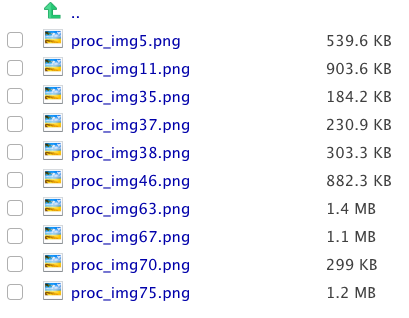
\includegraphics{imgs/pliman2.png}}

}

\caption{\label{fig-pliman2}Images created by pliman and exported to a
specific folder}

\end{figure}

Let's have a look at one of the processed images.

\begin{figure}

{\centering 

\href{fig_proc1}{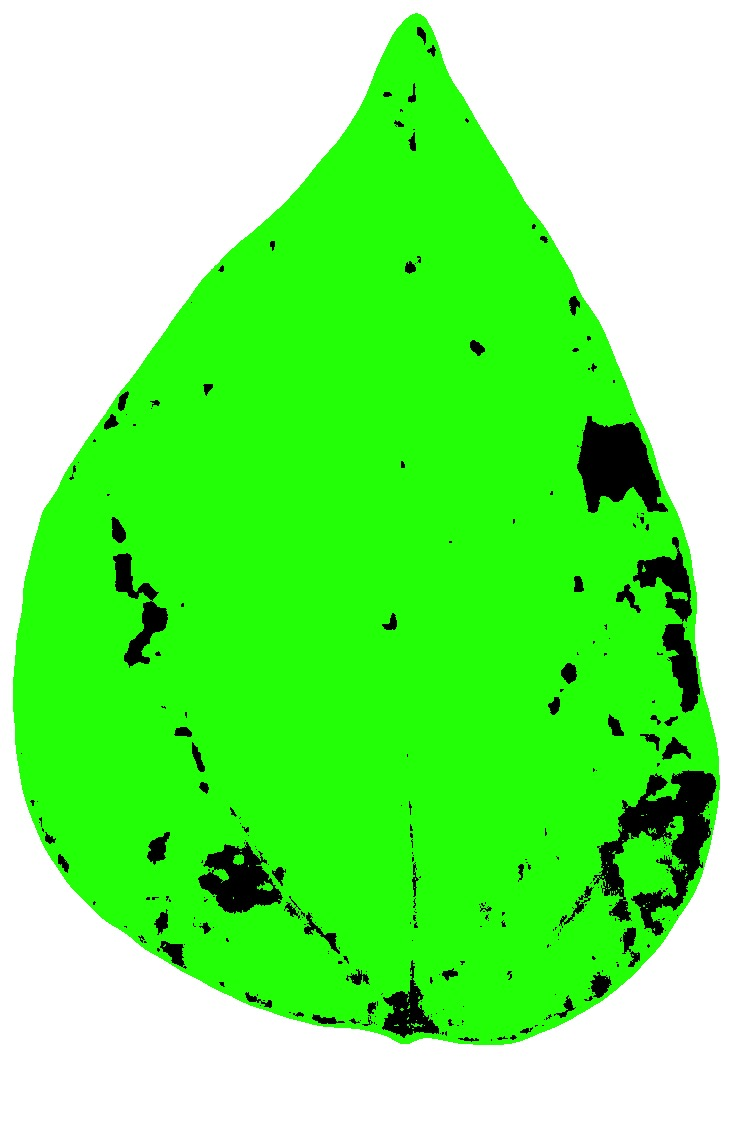
\includegraphics[width=4.70833in,height=\textheight]{imgs/processed/proc_img46.jpg}}

}

\caption{\label{fig-processed}Figure created by pliman after batch
processing to segment the images and calculate percent area covered by
symptoms. The symptomatic area is delinated in the image.}

\end{figure}

\hypertarget{more-than-a-target-per-image}{%
\subsubsection{More than a target per
image}\label{more-than-a-target-per-image}}

\{pliman\} offers a custom function to estimate the severity in multiple
targets (e.g.~leaf) per image. This is convenient to decrease the time
when scanning the specimens, for example. Let's combine three soybean
rust leaves into a single image and import it for processing. We will
further set the \texttt{index\_lb} (leaf background),
\texttt{save\_image} to \texttt{TRUE} and inform the directory for the
processed images using \texttt{dir\_processed}.

\begin{Shaded}
\begin{Highlighting}[]
\NormalTok{img2 }\OtherTok{\textless{}{-}} \FunctionTok{image\_import}\NormalTok{(}\StringTok{"imgs/soybean\_three.png"}\NormalTok{)}
\FunctionTok{image\_combine}\NormalTok{(img2)}
\end{Highlighting}
\end{Shaded}

\begin{figure}

\includegraphics{data-actual-severity_files/figure-latex/fig-img2-1.pdf} \hfill{}

\caption{\label{fig-img2}Imported image with multiple targets in a
single image for further analysis using measure\_disease\_byl() function
of the \{pliman\} package}

\end{figure}

\begin{Shaded}
\begin{Highlighting}[]
\NormalTok{ pliman2 }\OtherTok{\textless{}{-}} \FunctionTok{measure\_disease\_byl}\NormalTok{(}\AttributeTok{img =}\NormalTok{ img2,}
                        \AttributeTok{index\_lb =}\NormalTok{ b,}
                        \AttributeTok{img\_healthy =}\NormalTok{ h,}
                        \AttributeTok{img\_symptoms =}\NormalTok{ s, }
                        \AttributeTok{save\_image =} \ConstantTok{TRUE}\NormalTok{,}
                        \AttributeTok{dir\_processed =} \StringTok{"imgs/proc"}\NormalTok{)}
\end{Highlighting}
\end{Shaded}

\includegraphics{data-actual-severity_files/figure-latex/unnamed-chunk-11-1.pdf}

\includegraphics{data-actual-severity_files/figure-latex/unnamed-chunk-11-2.pdf}

\includegraphics{data-actual-severity_files/figure-latex/unnamed-chunk-11-3.pdf}

\begin{Shaded}
\begin{Highlighting}[]
\NormalTok{ pliman2}\SpecialCharTok{$}\NormalTok{severity}
\end{Highlighting}
\end{Shaded}

\begin{verbatim}
  img leaf  healthy symptomatic
1 img    1 59.11737   40.882632
2 img    2 61.36616   38.633841
3 img    3 93.21756    6.782436
\end{verbatim}

The original image is splited and the individual new images are saved in
the proc folder.

\begin{figure}

{\centering 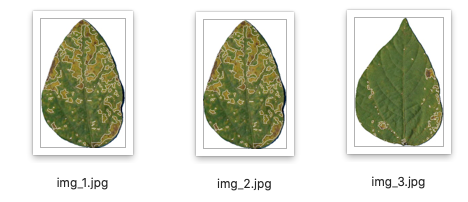
\includegraphics[width=5.26042in,height=\textheight]{imgs/sbr_procor.png}

}

\caption{Individual images of the soybean leaves after processed using
the measure\_disease\_byl function of the \{pliman\} package.}

\end{figure}

\hypertarget{how-good-are-these-measurements}{%
\section{How good are these
measurements?}\label{how-good-are-these-measurements}}

These 10 images were previously processed in QUANT software for
measuring severity which is also based on image threshold. Let's create
a tibble for the image code and respective ``actual'' severity -
assuming QUANT measures as reference.

\begin{Shaded}
\begin{Highlighting}[]
\FunctionTok{library}\NormalTok{(tidyverse)}
\FunctionTok{library}\NormalTok{(r4pde)}
\NormalTok{quant }\OtherTok{\textless{}{-}} \FunctionTok{tribble}\NormalTok{(}
  \SpecialCharTok{\textasciitilde{}}\NormalTok{img, }\SpecialCharTok{\textasciitilde{}}\NormalTok{actual,}
   \StringTok{"img5"}\NormalTok{,     }\DecValTok{75}\NormalTok{,}
  \StringTok{"img11"}\NormalTok{,     }\DecValTok{24}\NormalTok{,}
  \StringTok{"img35"}\NormalTok{,     }\DecValTok{52}\NormalTok{,}
  \StringTok{"img37"}\NormalTok{,     }\DecValTok{38}\NormalTok{,}
  \StringTok{"img38"}\NormalTok{,     }\DecValTok{17}\NormalTok{,}
  \StringTok{"img46"}\NormalTok{,      }\DecValTok{7}\NormalTok{,}
  \StringTok{"img63"}\NormalTok{,    }\FloatTok{2.5}\NormalTok{,}
  \StringTok{"img67"}\NormalTok{,   }\FloatTok{0.25}\NormalTok{,}
  \StringTok{"img70"}\NormalTok{,     }\DecValTok{67}\NormalTok{,}
  \StringTok{"img75"}\NormalTok{,     }\DecValTok{10}
\NormalTok{  )}
\end{Highlighting}
\end{Shaded}

We can now combine the two dataframes and produce a scatter plot
relating the two measures.

\begin{Shaded}
\begin{Highlighting}[]
\NormalTok{dat }\OtherTok{\textless{}{-}} \FunctionTok{left\_join}\NormalTok{(severity, quant)}
\end{Highlighting}
\end{Shaded}

\begin{verbatim}
Joining with `by = join_by(img)`
\end{verbatim}

\begin{Shaded}
\begin{Highlighting}[]
\NormalTok{dat }\SpecialCharTok{\%\textgreater{}\%}
  \FunctionTok{ggplot}\NormalTok{(}\FunctionTok{aes}\NormalTok{(actual, symptomatic)) }\SpecialCharTok{+}
  \FunctionTok{geom\_point}\NormalTok{(}\AttributeTok{size =} \DecValTok{3}\NormalTok{, }\AttributeTok{shape =} \DecValTok{16}\NormalTok{) }\SpecialCharTok{+}
  \FunctionTok{ylim}\NormalTok{(}\DecValTok{0}\NormalTok{, }\DecValTok{100}\NormalTok{) }\SpecialCharTok{+}
  \FunctionTok{xlim}\NormalTok{(}\DecValTok{0}\NormalTok{, }\DecValTok{100}\NormalTok{) }\SpecialCharTok{+}
  \FunctionTok{geom\_abline}\NormalTok{(}\AttributeTok{slope =} \DecValTok{1}\NormalTok{, }\AttributeTok{intercept =} \DecValTok{0}\NormalTok{) }\SpecialCharTok{+}
  \FunctionTok{labs}\NormalTok{(}\AttributeTok{x =} \StringTok{"Quant"}\NormalTok{,}
       \AttributeTok{y =} \StringTok{"pliman"}\NormalTok{)}\SpecialCharTok{+}
  \FunctionTok{theme\_r4pde}\NormalTok{()}
\end{Highlighting}
\end{Shaded}

\begin{figure}

\includegraphics{data-actual-severity_files/figure-latex/fig-scatter-1.pdf} \hfill{}

\caption{\label{fig-scatter}Scatter plot for the relationship between
severity values measured by pliman and Quant software}

\end{figure}

The concordance correlation coefficient is a test for agreement between
two observers or two methods (see previous chapter). It is an indication
of how accurate the \emph{pliman} measures are compared with a standard.
The coefficient is greater than 0.99 (1.0 is perfect concordance),
suggesting an excellent agreement!

\begin{Shaded}
\begin{Highlighting}[]
\FunctionTok{library}\NormalTok{(epiR)}
\NormalTok{ccc }\OtherTok{\textless{}{-}} \FunctionTok{epi.ccc}\NormalTok{(dat}\SpecialCharTok{$}\NormalTok{actual, dat}\SpecialCharTok{$}\NormalTok{symptomatic)}
\NormalTok{ccc}\SpecialCharTok{$}\NormalTok{rho.c}
\end{Highlighting}
\end{Shaded}

\begin{verbatim}
        est     lower     upper
1 0.9940835 0.9774587 0.9984566
\end{verbatim}

In conclusion, as mentioned earlier, the most critical step is defining
the reference image palettes. A few preliminary runs may be necessary
for some images to ensure that the segmentation is being carried out
correctly, based on visual judgment. This is not different from any
other color-threshold based methods, where the choices made by the user
impact the final result and contribute to variation among assessors. The
drawbacks are the same as those encountered with direct competitors,
namely, the need for images to be taken under uniform and controlled
conditions, especially with a contrasting background.

\hypertarget{creating-palettes-interactively}{%
\section{Creating palettes
interactively}\label{creating-palettes-interactively}}

Pliman offers another function \texttt{measure\_disease\_iter()} which
allows the user to pick up samples in the image to create the color
palettes for each required class (background, healthy and symptoms).
Check the video below.

\url{https://www.youtube.com/embed/fI_Mm-GlPyw}

\hypertarget{reliability-and-accuracy}{%
\chapter{Reliability and accuracy}\label{reliability-and-accuracy}}

\hypertarget{severity-data}{%
\chapter{Severity data}\label{severity-data}}

\hypertarget{terminology}{%
\section{Terminology}\label{terminology}}

Disease severity, mainly when expressed in percent area diseased
assessed visually, is acknowledged as a more difficult and less time-
and cost-effective plant disease variable to obtain. However, errors may
occur even when assessing a more objective measure such as incidence.
This is the case when an incorrect assignment or confusion of symptoms
occur. In either case, the quality of the assessment of any disease
variable is very important and should be gauged in the studies. Several
terms can be used when evaluating the quality of disease assessments,
including reliability, precision, accuracy or agreement.

\textbf{Reliability}: The extent to which the same estimates or
measurements of diseased specimens obtained under different conditions
yield similar results. There are two types. The \emph{inter-rater
reliability} (or reproducibility) is a measure of consistency of disease
assessment across the same specimens between raters or devices. The
\emph{intra-rater} reliability (or repeatability) measures consistency
by the same rater or instrument on the same specimens (e.g.~two
assessments in time by the same rater).

\begin{figure}

{\centering 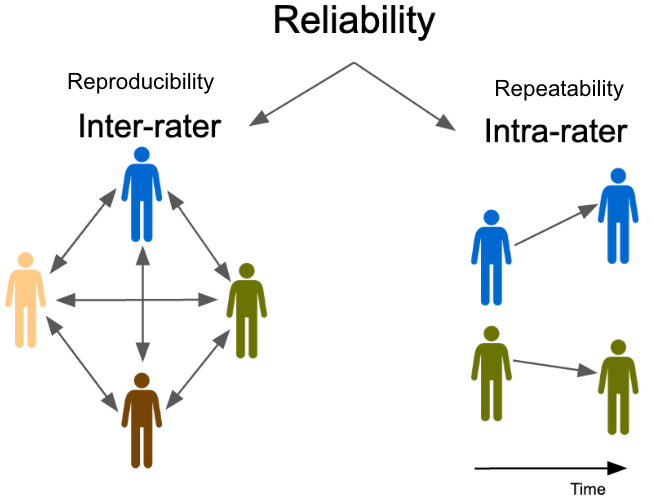
\includegraphics[width=5.26042in,height=\textheight]{imgs/reliability.png}

}

\caption{\label{fig-reliability.png}Two types of reliability of
estimates or measures of plant disease intensity}

\end{figure}

\textbf{Precision:} A statistical term to express the measure of
variability of the estimates or measurements of disease on the same
specimens obtained by different raters (or instruments). However,
reliable or precise estimates (or measurements) are not necessarily
close to an actual value, but precision is a component of accuracy or
agreement.

\textbf{Accuracy or agreement}: These two terms can be treated as
synonymous in plant pathological research. They refer to the closeness
(or concordance) of an estimate or measurement to the actual severity
value for a specimen on the same scale. Actual values may be obtained
using various methods, against which estimates or measurements using an
experimental assessment method are compared.

An analogy commonly used to explain accuracy and precision is the archer
shooting arrows at a target and trying to hit the bull's eye (center of
the target) with each of five arrows. The figure below is used to
demonstrate four situations from the combination of two levels (high and
low) for precision and accuracy. The figure was produced using the
\texttt{ggplot} function of \emph{ggplot2} package.

\begin{Shaded}
\begin{Highlighting}[]
\FunctionTok{library}\NormalTok{(ggplot2)}
\NormalTok{target }\OtherTok{\textless{}{-}} 
  \FunctionTok{ggplot}\NormalTok{(}\FunctionTok{data.frame}\NormalTok{(}\FunctionTok{c}\NormalTok{(}\DecValTok{1}\SpecialCharTok{:}\DecValTok{10}\NormalTok{),}\FunctionTok{c}\NormalTok{(}\DecValTok{1}\SpecialCharTok{:}\DecValTok{10}\NormalTok{)))}\SpecialCharTok{+}
  \FunctionTok{geom\_point}\NormalTok{(}\FunctionTok{aes}\NormalTok{(}\AttributeTok{x =} \DecValTok{5}\NormalTok{, }\AttributeTok{y =} \DecValTok{5}\NormalTok{), }\AttributeTok{size =} \FloatTok{71.5}\NormalTok{, }\AttributeTok{color =} \StringTok{"black"}\NormalTok{)}\SpecialCharTok{+}
  \FunctionTok{geom\_point}\NormalTok{(}\FunctionTok{aes}\NormalTok{(}\AttributeTok{x =} \DecValTok{5}\NormalTok{, }\AttributeTok{y =} \DecValTok{5}\NormalTok{), }\AttributeTok{size =} \DecValTok{70}\NormalTok{, }\AttributeTok{color =} \StringTok{"\#99cc66"}\NormalTok{)}\SpecialCharTok{+}
  \FunctionTok{geom\_point}\NormalTok{(}\FunctionTok{aes}\NormalTok{(}\AttributeTok{x =} \DecValTok{5}\NormalTok{, }\AttributeTok{y =} \DecValTok{5}\NormalTok{), }\AttributeTok{size =} \DecValTok{60}\NormalTok{, }\AttributeTok{color =} \StringTok{"white"}\NormalTok{)}\SpecialCharTok{+}
  \FunctionTok{geom\_point}\NormalTok{(}\FunctionTok{aes}\NormalTok{(}\AttributeTok{x =} \DecValTok{5}\NormalTok{, }\AttributeTok{y =} \DecValTok{5}\NormalTok{), }\AttributeTok{size =} \DecValTok{50}\NormalTok{, }\AttributeTok{color =} \StringTok{"\#99cc66"}\NormalTok{)}\SpecialCharTok{+}
  \FunctionTok{geom\_point}\NormalTok{(}\FunctionTok{aes}\NormalTok{(}\AttributeTok{x =} \DecValTok{5}\NormalTok{, }\AttributeTok{y =} \DecValTok{5}\NormalTok{), }\AttributeTok{size =} \DecValTok{40}\NormalTok{, }\AttributeTok{color =} \StringTok{"white"}\NormalTok{)}\SpecialCharTok{+}
  \FunctionTok{geom\_point}\NormalTok{(}\FunctionTok{aes}\NormalTok{(}\AttributeTok{x =} \DecValTok{5}\NormalTok{, }\AttributeTok{y =} \DecValTok{5}\NormalTok{), }\AttributeTok{size =} \DecValTok{30}\NormalTok{, }\AttributeTok{color =} \StringTok{"\#99cc66"}\NormalTok{)}\SpecialCharTok{+}
  \FunctionTok{geom\_point}\NormalTok{(}\FunctionTok{aes}\NormalTok{(}\AttributeTok{x =} \DecValTok{5}\NormalTok{, }\AttributeTok{y =} \DecValTok{5}\NormalTok{), }\AttributeTok{size =} \DecValTok{20}\NormalTok{, }\AttributeTok{color =} \StringTok{"white"}\NormalTok{)}\SpecialCharTok{+}
  \FunctionTok{geom\_point}\NormalTok{(}\FunctionTok{aes}\NormalTok{(}\AttributeTok{x =} \DecValTok{5}\NormalTok{, }\AttributeTok{y =} \DecValTok{5}\NormalTok{), }\AttributeTok{size =} \DecValTok{10}\NormalTok{, }\AttributeTok{color =} \StringTok{"\#99cc66"}\NormalTok{)}\SpecialCharTok{+}
  \FunctionTok{geom\_point}\NormalTok{(}\FunctionTok{aes}\NormalTok{(}\AttributeTok{x =} \DecValTok{5}\NormalTok{, }\AttributeTok{y =} \DecValTok{5}\NormalTok{), }\AttributeTok{size =} \DecValTok{4}\NormalTok{, }\AttributeTok{color =} \StringTok{"white"}\NormalTok{)}\SpecialCharTok{+}
  \FunctionTok{ylim}\NormalTok{(}\DecValTok{0}\NormalTok{,}\DecValTok{10}\NormalTok{)}\SpecialCharTok{+}
  \FunctionTok{xlim}\NormalTok{(}\DecValTok{0}\NormalTok{,}\DecValTok{10}\NormalTok{)}\SpecialCharTok{+}
  \FunctionTok{theme\_void}\NormalTok{()}

\NormalTok{hahp }\OtherTok{\textless{}{-}}\NormalTok{ target }\SpecialCharTok{+}
  \FunctionTok{labs}\NormalTok{(}\AttributeTok{subtitle =} \StringTok{"High Accuracy High Precision"}\NormalTok{)}\SpecialCharTok{+}
  \FunctionTok{theme}\NormalTok{(}\AttributeTok{plot.subtitle =} \FunctionTok{element\_text}\NormalTok{(}\AttributeTok{hjust =} \FloatTok{0.5}\NormalTok{))}\SpecialCharTok{+}
  \FunctionTok{geom\_point}\NormalTok{(}\FunctionTok{aes}\NormalTok{(}\AttributeTok{x =} \DecValTok{5}\NormalTok{, }\AttributeTok{y =} \DecValTok{5}\NormalTok{), }\AttributeTok{shape =} \DecValTok{4}\NormalTok{, }\AttributeTok{size =}\DecValTok{2}\NormalTok{, }\AttributeTok{color =} \StringTok{"blue"}\NormalTok{)}\SpecialCharTok{+}
  \FunctionTok{geom\_point}\NormalTok{(}\FunctionTok{aes}\NormalTok{(}\AttributeTok{x =} \DecValTok{5}\NormalTok{, }\AttributeTok{y =} \FloatTok{5.2}\NormalTok{), }\AttributeTok{shape =} \DecValTok{4}\NormalTok{, }\AttributeTok{size =}\DecValTok{2}\NormalTok{, }\AttributeTok{color =} \StringTok{"blue"}\NormalTok{)}\SpecialCharTok{+}
  \FunctionTok{geom\_point}\NormalTok{(}\FunctionTok{aes}\NormalTok{(}\AttributeTok{x =} \DecValTok{5}\NormalTok{, }\AttributeTok{y =} \FloatTok{4.8}\NormalTok{), }\AttributeTok{shape =} \DecValTok{4}\NormalTok{, }\AttributeTok{size =}\DecValTok{2}\NormalTok{, }\AttributeTok{color =} \StringTok{"blue"}\NormalTok{)}\SpecialCharTok{+}
  \FunctionTok{geom\_point}\NormalTok{(}\FunctionTok{aes}\NormalTok{(}\AttributeTok{x =} \FloatTok{4.8}\NormalTok{, }\AttributeTok{y =} \DecValTok{5}\NormalTok{), }\AttributeTok{shape =} \DecValTok{4}\NormalTok{, }\AttributeTok{size =}\DecValTok{2}\NormalTok{, }\AttributeTok{color =} \StringTok{"blue"}\NormalTok{)}\SpecialCharTok{+}
  \FunctionTok{geom\_point}\NormalTok{(}\FunctionTok{aes}\NormalTok{(}\AttributeTok{x =} \FloatTok{5.2}\NormalTok{, }\AttributeTok{y =} \DecValTok{5}\NormalTok{), }\AttributeTok{shape =} \DecValTok{4}\NormalTok{, }\AttributeTok{size =}\DecValTok{2}\NormalTok{, }\AttributeTok{color =} \StringTok{"blue"}\NormalTok{)}


\NormalTok{lahp }\OtherTok{\textless{}{-}}\NormalTok{ target }\SpecialCharTok{+}
  \FunctionTok{labs}\NormalTok{(}\AttributeTok{subtitle =} \StringTok{"Low Accuracy High Precision"}\NormalTok{)}\SpecialCharTok{+}
  \FunctionTok{theme}\NormalTok{(}\AttributeTok{plot.subtitle =} \FunctionTok{element\_text}\NormalTok{(}\AttributeTok{hjust =} \FloatTok{0.5}\NormalTok{))}\SpecialCharTok{+}
  \FunctionTok{geom\_point}\NormalTok{(}\FunctionTok{aes}\NormalTok{(}\AttributeTok{x =} \DecValTok{6}\NormalTok{, }\AttributeTok{y =} \DecValTok{6}\NormalTok{), }\AttributeTok{shape =} \DecValTok{4}\NormalTok{, }\AttributeTok{size =}\DecValTok{2}\NormalTok{, }\AttributeTok{color =} \StringTok{"blue"}\NormalTok{)}\SpecialCharTok{+}
  \FunctionTok{geom\_point}\NormalTok{(}\FunctionTok{aes}\NormalTok{(}\AttributeTok{x =} \DecValTok{6}\NormalTok{, }\AttributeTok{y =} \FloatTok{6.2}\NormalTok{), }\AttributeTok{shape =} \DecValTok{4}\NormalTok{, }\AttributeTok{size =}\DecValTok{2}\NormalTok{, }\AttributeTok{color =} \StringTok{"blue"}\NormalTok{)}\SpecialCharTok{+}
  \FunctionTok{geom\_point}\NormalTok{(}\FunctionTok{aes}\NormalTok{(}\AttributeTok{x =} \DecValTok{6}\NormalTok{, }\AttributeTok{y =} \FloatTok{5.8}\NormalTok{), }\AttributeTok{shape =} \DecValTok{4}\NormalTok{, }\AttributeTok{size =}\DecValTok{2}\NormalTok{, }\AttributeTok{color =} \StringTok{"blue"}\NormalTok{)}\SpecialCharTok{+}
  \FunctionTok{geom\_point}\NormalTok{(}\FunctionTok{aes}\NormalTok{(}\AttributeTok{x =} \FloatTok{5.8}\NormalTok{, }\AttributeTok{y =} \DecValTok{6}\NormalTok{), }\AttributeTok{shape =} \DecValTok{4}\NormalTok{, }\AttributeTok{size =}\DecValTok{2}\NormalTok{, }\AttributeTok{color =} \StringTok{"blue"}\NormalTok{)}\SpecialCharTok{+}
  \FunctionTok{geom\_point}\NormalTok{(}\FunctionTok{aes}\NormalTok{(}\AttributeTok{x =} \FloatTok{6.2}\NormalTok{, }\AttributeTok{y =} \DecValTok{6}\NormalTok{), }\AttributeTok{shape =} \DecValTok{4}\NormalTok{, }\AttributeTok{size =}\DecValTok{2}\NormalTok{, }\AttributeTok{color =} \StringTok{"blue"}\NormalTok{)}


\NormalTok{halp }\OtherTok{\textless{}{-}}\NormalTok{ target }\SpecialCharTok{+}
  \FunctionTok{labs}\NormalTok{(}\AttributeTok{subtitle =} \StringTok{"High Accuracy Low Precision"}\NormalTok{)}\SpecialCharTok{+}
  \FunctionTok{theme}\NormalTok{(}\AttributeTok{plot.subtitle =} \FunctionTok{element\_text}\NormalTok{(}\AttributeTok{hjust =} \FloatTok{0.5}\NormalTok{))}\SpecialCharTok{+}
  \FunctionTok{geom\_point}\NormalTok{(}\FunctionTok{aes}\NormalTok{(}\AttributeTok{x =} \DecValTok{5}\NormalTok{, }\AttributeTok{y =} \DecValTok{5}\NormalTok{), }\AttributeTok{shape =} \DecValTok{4}\NormalTok{, }\AttributeTok{size =}\DecValTok{2}\NormalTok{, }\AttributeTok{color =} \StringTok{"blue"}\NormalTok{)}\SpecialCharTok{+}
  \FunctionTok{geom\_point}\NormalTok{(}\FunctionTok{aes}\NormalTok{(}\AttributeTok{x =} \DecValTok{5}\NormalTok{, }\AttributeTok{y =} \FloatTok{5.8}\NormalTok{), }\AttributeTok{shape =} \DecValTok{4}\NormalTok{, }\AttributeTok{size =}\DecValTok{2}\NormalTok{, }\AttributeTok{color =} \StringTok{"blue"}\NormalTok{)}\SpecialCharTok{+}
  \FunctionTok{geom\_point}\NormalTok{(}\FunctionTok{aes}\NormalTok{(}\AttributeTok{x =} \FloatTok{5.8}\NormalTok{, }\AttributeTok{y =} \FloatTok{4.4}\NormalTok{), }\AttributeTok{shape =} \DecValTok{4}\NormalTok{, }\AttributeTok{size =}\DecValTok{2}\NormalTok{, }\AttributeTok{color =} \StringTok{"blue"}\NormalTok{)}\SpecialCharTok{+}
  \FunctionTok{geom\_point}\NormalTok{(}\FunctionTok{aes}\NormalTok{(}\AttributeTok{x =} \FloatTok{4.4}\NormalTok{, }\AttributeTok{y =} \DecValTok{5}\NormalTok{), }\AttributeTok{shape =} \DecValTok{4}\NormalTok{, }\AttributeTok{size =}\DecValTok{2}\NormalTok{, }\AttributeTok{color =} \StringTok{"blue"}\NormalTok{)}\SpecialCharTok{+}
  \FunctionTok{geom\_point}\NormalTok{(}\FunctionTok{aes}\NormalTok{(}\AttributeTok{x =} \FloatTok{5.6}\NormalTok{, }\AttributeTok{y =} \FloatTok{5.6}\NormalTok{), }\AttributeTok{shape =} \DecValTok{4}\NormalTok{, }\AttributeTok{size =}\DecValTok{2}\NormalTok{, }\AttributeTok{color =} \StringTok{"blue"}\NormalTok{)}

\NormalTok{lalp }\OtherTok{\textless{}{-}}\NormalTok{ target }\SpecialCharTok{+}
  \FunctionTok{labs}\NormalTok{(}\AttributeTok{subtitle =} \StringTok{"Low Accuracy Low Precision"}\NormalTok{)}\SpecialCharTok{+}
  \FunctionTok{theme}\NormalTok{(}\AttributeTok{plot.subtitle =} \FunctionTok{element\_text}\NormalTok{(}\AttributeTok{hjust =} \FloatTok{0.5}\NormalTok{))}\SpecialCharTok{+}
  \FunctionTok{geom\_point}\NormalTok{(}\FunctionTok{aes}\NormalTok{(}\AttributeTok{x =} \FloatTok{5.5}\NormalTok{, }\AttributeTok{y =} \FloatTok{5.5}\NormalTok{), }\AttributeTok{shape =} \DecValTok{4}\NormalTok{, }\AttributeTok{size =}\DecValTok{2}\NormalTok{, }\AttributeTok{color =} \StringTok{"blue"}\NormalTok{)}\SpecialCharTok{+}
  \FunctionTok{geom\_point}\NormalTok{(}\FunctionTok{aes}\NormalTok{(}\AttributeTok{x =} \FloatTok{4.5}\NormalTok{, }\AttributeTok{y =} \FloatTok{5.4}\NormalTok{), }\AttributeTok{shape =} \DecValTok{4}\NormalTok{, }\AttributeTok{size =}\DecValTok{2}\NormalTok{, }\AttributeTok{color =} \StringTok{"blue"}\NormalTok{)}\SpecialCharTok{+}
  \FunctionTok{geom\_point}\NormalTok{(}\FunctionTok{aes}\NormalTok{(}\AttributeTok{x =} \FloatTok{5.2}\NormalTok{, }\AttributeTok{y =} \FloatTok{6.8}\NormalTok{), }\AttributeTok{shape =} \DecValTok{4}\NormalTok{, }\AttributeTok{size =}\DecValTok{2}\NormalTok{, }\AttributeTok{color =} \StringTok{"blue"}\NormalTok{)}\SpecialCharTok{+}
  \FunctionTok{geom\_point}\NormalTok{(}\FunctionTok{aes}\NormalTok{(}\AttributeTok{x =} \FloatTok{4.8}\NormalTok{, }\AttributeTok{y =} \FloatTok{3.8}\NormalTok{), }\AttributeTok{shape =} \DecValTok{4}\NormalTok{, }\AttributeTok{size =}\DecValTok{2}\NormalTok{, }\AttributeTok{color =} \StringTok{"blue"}\NormalTok{)}\SpecialCharTok{+}
  \FunctionTok{geom\_point}\NormalTok{(}\FunctionTok{aes}\NormalTok{(}\AttributeTok{x =} \FloatTok{5.2}\NormalTok{, }\AttributeTok{y =} \DecValTok{3}\NormalTok{), }\AttributeTok{shape =} \DecValTok{4}\NormalTok{, }\AttributeTok{size =}\DecValTok{2}\NormalTok{, }\AttributeTok{color =} \StringTok{"blue"}\NormalTok{)}


\FunctionTok{library}\NormalTok{(patchwork)}
\NormalTok{(hahp }\SpecialCharTok{|}\NormalTok{ lahp) }\SpecialCharTok{/}
\NormalTok{(halp }\SpecialCharTok{|}\NormalTok{ lalp)}
\end{Highlighting}
\end{Shaded}

\begin{figure}

\includegraphics{data-accuracy_files/figure-latex/fig-target-1.pdf} \hfill{}

\caption{\label{fig-target}The accuracy and precision of the archer is
determined by the location of the group of arrows}

\end{figure}

Another way to visualize accuracy and precision is via scatter plots for
the relationship between the actual values and the estimates.

\begin{Shaded}
\begin{Highlighting}[]
\FunctionTok{library}\NormalTok{(tidyverse)}
\FunctionTok{library}\NormalTok{(r4pde)}
\FunctionTok{theme\_set}\NormalTok{(}\FunctionTok{theme\_r4pde}\NormalTok{())}
\NormalTok{dat }\OtherTok{\textless{}{-}} 
\NormalTok{tibble}\SpecialCharTok{::}\FunctionTok{tribble}\NormalTok{(}
  \SpecialCharTok{\textasciitilde{}}\NormalTok{actual,   }\SpecialCharTok{\textasciitilde{}}\NormalTok{ap,   }\SpecialCharTok{\textasciitilde{}}\NormalTok{ip,   }\SpecialCharTok{\textasciitilde{}}\NormalTok{ai,   }\SpecialCharTok{\textasciitilde{}}\NormalTok{ii,}
        \DecValTok{0}\NormalTok{,     }\DecValTok{0}\NormalTok{,    }\DecValTok{10}\NormalTok{,     }\DecValTok{0}\NormalTok{,    }\DecValTok{25}\NormalTok{,}
       \DecValTok{10}\NormalTok{,    }\DecValTok{10}\NormalTok{,    }\DecValTok{20}\NormalTok{,     }\DecValTok{5}\NormalTok{,    }\DecValTok{10}\NormalTok{,}
       \DecValTok{20}\NormalTok{,    }\DecValTok{20}\NormalTok{,    }\DecValTok{30}\NormalTok{,    }\DecValTok{30}\NormalTok{,    }\DecValTok{10}\NormalTok{,}
       \DecValTok{30}\NormalTok{,    }\DecValTok{30}\NormalTok{,    }\DecValTok{40}\NormalTok{,    }\DecValTok{30}\NormalTok{,    }\DecValTok{45}\NormalTok{,}
       \DecValTok{40}\NormalTok{,    }\DecValTok{40}\NormalTok{,    }\DecValTok{50}\NormalTok{,    }\DecValTok{30}\NormalTok{,    }\DecValTok{35}\NormalTok{,}
       \DecValTok{50}\NormalTok{,    }\DecValTok{50}\NormalTok{,    }\DecValTok{60}\NormalTok{,    }\DecValTok{60}\NormalTok{,    }\DecValTok{65}\NormalTok{,}
       \DecValTok{60}\NormalTok{,    }\DecValTok{60}\NormalTok{,    }\DecValTok{70}\NormalTok{,    }\DecValTok{50}\NormalTok{,    }\DecValTok{30}
\NormalTok{  )}

\NormalTok{ap }\OtherTok{\textless{}{-}}\NormalTok{ dat }\SpecialCharTok{|\textgreater{}} 
  \FunctionTok{ggplot}\NormalTok{(}\FunctionTok{aes}\NormalTok{(actual, ap))}\SpecialCharTok{+}
  \FunctionTok{geom\_abline}\NormalTok{(}\AttributeTok{intercept =} \DecValTok{0}\NormalTok{, }\AttributeTok{slope =} \DecValTok{1}\NormalTok{, }
              \AttributeTok{linetype =} \DecValTok{2}\NormalTok{, }\AttributeTok{size =} \DecValTok{1}\NormalTok{)}\SpecialCharTok{+}
    \FunctionTok{geom\_smooth}\NormalTok{(}\AttributeTok{method =} \StringTok{"lm"}\NormalTok{)}\SpecialCharTok{+}
   \FunctionTok{geom\_point}\NormalTok{(}\AttributeTok{color =} \StringTok{"\#99cc66"}\NormalTok{, }\AttributeTok{size =} \DecValTok{3}\NormalTok{)}\SpecialCharTok{+}
   \FunctionTok{ylim}\NormalTok{(}\DecValTok{0}\NormalTok{,}\DecValTok{70}\NormalTok{)}\SpecialCharTok{+}
  \FunctionTok{xlim}\NormalTok{(}\DecValTok{0}\NormalTok{,}\DecValTok{70}\NormalTok{)}\SpecialCharTok{+}
  \FunctionTok{labs}\NormalTok{(}\AttributeTok{x =} \StringTok{"Actual"}\NormalTok{, }\AttributeTok{y =} \StringTok{"Estimate"}\NormalTok{,}
       \AttributeTok{subtitle =} \StringTok{"High Acccuracy High Precision"}\NormalTok{)}

\NormalTok{ip }\OtherTok{\textless{}{-}}\NormalTok{ dat }\SpecialCharTok{|\textgreater{}} 
  \FunctionTok{ggplot}\NormalTok{(}\FunctionTok{aes}\NormalTok{(actual, ip))}\SpecialCharTok{+}
  \FunctionTok{geom\_abline}\NormalTok{(}\AttributeTok{intercept =} \DecValTok{0}\NormalTok{, }\AttributeTok{slope =} \DecValTok{1}\NormalTok{, }
              \AttributeTok{linetype =} \DecValTok{2}\NormalTok{, }\AttributeTok{size =} \DecValTok{1}\NormalTok{)}\SpecialCharTok{+}
  \FunctionTok{geom\_smooth}\NormalTok{(}\AttributeTok{method =} \StringTok{"lm"}\NormalTok{, }\AttributeTok{se =}\NormalTok{ F)}\SpecialCharTok{+}
  \FunctionTok{geom\_point}\NormalTok{(}\AttributeTok{color =} \StringTok{"\#99cc66"}\NormalTok{, }\AttributeTok{size =} \DecValTok{3}\NormalTok{)}\SpecialCharTok{+}
  \FunctionTok{ylim}\NormalTok{(}\DecValTok{0}\NormalTok{,}\DecValTok{70}\NormalTok{)}\SpecialCharTok{+}
  \FunctionTok{xlim}\NormalTok{(}\DecValTok{0}\NormalTok{,}\DecValTok{70}\NormalTok{)}\SpecialCharTok{+}
  \FunctionTok{labs}\NormalTok{(}\AttributeTok{x =} \StringTok{"Actual"}\NormalTok{, }\AttributeTok{y =} \StringTok{"Estimate"}\NormalTok{,}
       \AttributeTok{subtitle =} \StringTok{"Low Acccuracy High Precision"}\NormalTok{)}

\NormalTok{ai }\OtherTok{\textless{}{-}}\NormalTok{ dat }\SpecialCharTok{|\textgreater{}} 
  \FunctionTok{ggplot}\NormalTok{(}\FunctionTok{aes}\NormalTok{(actual, ai))}\SpecialCharTok{+}
  \FunctionTok{geom\_abline}\NormalTok{(}\AttributeTok{intercept =} \DecValTok{0}\NormalTok{, }\AttributeTok{slope =} \DecValTok{1}\NormalTok{, }
              \AttributeTok{linetype =} \DecValTok{2}\NormalTok{, }\AttributeTok{size =} \DecValTok{1}\NormalTok{)}\SpecialCharTok{+}
  \FunctionTok{geom\_smooth}\NormalTok{(}\AttributeTok{method =} \StringTok{"lm"}\NormalTok{, }\AttributeTok{se =}\NormalTok{ F)}\SpecialCharTok{+}
  \FunctionTok{geom\_point}\NormalTok{(}\AttributeTok{color =} \StringTok{"\#99cc66"}\NormalTok{, }\AttributeTok{size =} \DecValTok{3}\NormalTok{)}\SpecialCharTok{+}
  \FunctionTok{ylim}\NormalTok{(}\DecValTok{0}\NormalTok{,}\DecValTok{70}\NormalTok{)}\SpecialCharTok{+}
  \FunctionTok{xlim}\NormalTok{(}\DecValTok{0}\NormalTok{,}\DecValTok{70}\NormalTok{)}\SpecialCharTok{+}
  \FunctionTok{labs}\NormalTok{(}\AttributeTok{x =} \StringTok{"Actual"}\NormalTok{, }\AttributeTok{y =} \StringTok{"Estimate"}\NormalTok{,}
       \AttributeTok{subtitle =} \StringTok{"High Acccuracy Low precision"}\NormalTok{)}

\NormalTok{ii }\OtherTok{\textless{}{-}}\NormalTok{ dat }\SpecialCharTok{|\textgreater{}} 
  \FunctionTok{ggplot}\NormalTok{(}\FunctionTok{aes}\NormalTok{(actual, ii))}\SpecialCharTok{+}
  \FunctionTok{geom\_abline}\NormalTok{(}\AttributeTok{intercept =} \DecValTok{0}\NormalTok{, }\AttributeTok{slope =} \DecValTok{1}\NormalTok{, }
              \AttributeTok{linetype =} \DecValTok{2}\NormalTok{, }\AttributeTok{size =} \DecValTok{1}\NormalTok{)}\SpecialCharTok{+}
  \FunctionTok{geom\_smooth}\NormalTok{(}\AttributeTok{method =} \StringTok{"lm"}\NormalTok{, }\AttributeTok{se =}\NormalTok{ F)}\SpecialCharTok{+}
  \FunctionTok{geom\_point}\NormalTok{(}\AttributeTok{color =} \StringTok{"\#99cc66"}\NormalTok{, }\AttributeTok{size =} \DecValTok{3}\NormalTok{)}\SpecialCharTok{+}
  \FunctionTok{ylim}\NormalTok{(}\DecValTok{0}\NormalTok{,}\DecValTok{70}\NormalTok{)}\SpecialCharTok{+}
  \FunctionTok{xlim}\NormalTok{(}\DecValTok{0}\NormalTok{,}\DecValTok{70}\NormalTok{)}\SpecialCharTok{+}
  \FunctionTok{labs}\NormalTok{(}\AttributeTok{x =} \StringTok{"Actual"}\NormalTok{, }\AttributeTok{y =} \StringTok{"Estimate"}\NormalTok{,}
       \AttributeTok{subtitle =} \StringTok{"Low Acccuracy Low Precision"}\NormalTok{)}

\FunctionTok{library}\NormalTok{(patchwork)}
\NormalTok{(ap }\SpecialCharTok{|}\NormalTok{ ip) }\SpecialCharTok{/}\NormalTok{ (ai }\SpecialCharTok{|}\NormalTok{ ii)}
\end{Highlighting}
\end{Shaded}

\begin{figure}

\includegraphics{data-accuracy_files/figure-latex/fig-accuracy-1.pdf} \hfill{}

\caption{\label{fig-accuracy}Scatter plots for the relationship between
actual and estimated values representing situations of low or high
precision and accuracy. The dashed line indicates the perfect
concordance and the solid blue line represents the fit of the linear
regression model}

\end{figure}

\hypertarget{statistical-summaries}{%
\section{Statistical summaries}\label{statistical-summaries}}

A formal assessment of the quality of estimates or measures is made
using statistical summaries of the data expressed as indices that
represent reliability, precision and accuracy. These indices can further
be used to test hypothesis such as if one or another method is superior
than the other. The indices or the tests vary according to the nature of
the variable, whether continuous, binary or categorical.

\hypertarget{inter-rater-reliability}{%
\subsection{Inter-rater reliability}\label{inter-rater-reliability}}

To calculate measures of inter-rater reliability (or reproducibility) we
will work with a fraction of a larger dataset used in a published
\href{https://bsppjournals.onlinelibrary.wiley.com/doi/abs/10.1111/ppa.13148}{study}.
There, the authors tested the effect of standard area diagrams (SADs) on
the reliability and accuracy of visual estimates of severity of soybean
rust.

The selected dataset consists of five columns with 20 rows. The first is
the leaf number and the others correspond to assessments of percent
soybean rust severity by four raters (R1 to R4). Each row correspond to
one symptomatic leaf. Let's assign the tibble to a dataframe called
\texttt{sbr} (an acronym for soybean rust). Note that the variable is
continuous.

\begin{Shaded}
\begin{Highlighting}[]
\FunctionTok{library}\NormalTok{(tidyverse)}
\NormalTok{sbr }\OtherTok{\textless{}{-}} \FunctionTok{tribble}\NormalTok{(}
\SpecialCharTok{\textasciitilde{}}\NormalTok{leaf, }\SpecialCharTok{\textasciitilde{}}\NormalTok{R1, }\SpecialCharTok{\textasciitilde{}}\NormalTok{R2,  }\SpecialCharTok{\textasciitilde{}}\NormalTok{R3, }\SpecialCharTok{\textasciitilde{}}\NormalTok{R4,}
\DecValTok{1}\NormalTok{, }\FloatTok{0.6}\NormalTok{, }\FloatTok{0.6}\NormalTok{,  }\FloatTok{0.7}\NormalTok{, }\FloatTok{0.6}\NormalTok{,}
\DecValTok{2}\NormalTok{,   }\DecValTok{2}\NormalTok{, }\FloatTok{0.7}\NormalTok{,    }\DecValTok{5}\NormalTok{,   }\DecValTok{1}\NormalTok{,}
\DecValTok{3}\NormalTok{,   }\DecValTok{5}\NormalTok{,   }\DecValTok{5}\NormalTok{,    }\DecValTok{8}\NormalTok{,   }\DecValTok{5}\NormalTok{,}
\DecValTok{4}\NormalTok{,   }\DecValTok{2}\NormalTok{,   }\DecValTok{4}\NormalTok{,    }\DecValTok{6}\NormalTok{,   }\DecValTok{2}\NormalTok{,}
\DecValTok{5}\NormalTok{,   }\DecValTok{6}\NormalTok{,  }\DecValTok{14}\NormalTok{,   }\DecValTok{10}\NormalTok{,   }\DecValTok{7}\NormalTok{,}
\DecValTok{6}\NormalTok{,   }\DecValTok{5}\NormalTok{,   }\DecValTok{6}\NormalTok{,   }\DecValTok{10}\NormalTok{,   }\DecValTok{5}\NormalTok{,}
\DecValTok{7}\NormalTok{,  }\DecValTok{10}\NormalTok{,  }\DecValTok{18}\NormalTok{, }\FloatTok{12.5}\NormalTok{,  }\DecValTok{12}\NormalTok{,}
\DecValTok{8}\NormalTok{,  }\DecValTok{15}\NormalTok{,  }\DecValTok{30}\NormalTok{,   }\DecValTok{22}\NormalTok{,  }\DecValTok{10}\NormalTok{,}
\DecValTok{9}\NormalTok{,   }\DecValTok{7}\NormalTok{,   }\DecValTok{2}\NormalTok{,   }\DecValTok{12}\NormalTok{,   }\DecValTok{8}\NormalTok{,}
\DecValTok{10}\NormalTok{,  }\DecValTok{6}\NormalTok{,   }\DecValTok{9}\NormalTok{, }\FloatTok{11.5}\NormalTok{,   }\DecValTok{8}\NormalTok{,}
\DecValTok{11}\NormalTok{,  }\DecValTok{7}\NormalTok{,   }\DecValTok{7}\NormalTok{,   }\DecValTok{20}\NormalTok{,   }\DecValTok{9}\NormalTok{,}
\DecValTok{12}\NormalTok{,  }\DecValTok{6}\NormalTok{,  }\DecValTok{23}\NormalTok{,   }\DecValTok{22}\NormalTok{,  }\DecValTok{14}\NormalTok{,}
\DecValTok{13}\NormalTok{, }\DecValTok{10}\NormalTok{,  }\DecValTok{35}\NormalTok{, }\FloatTok{18.5}\NormalTok{,  }\DecValTok{20}\NormalTok{,}
\DecValTok{14}\NormalTok{, }\DecValTok{19}\NormalTok{,  }\DecValTok{10}\NormalTok{,    }\DecValTok{9}\NormalTok{,  }\DecValTok{10}\NormalTok{,}
\DecValTok{15}\NormalTok{, }\DecValTok{15}\NormalTok{,  }\DecValTok{20}\NormalTok{,   }\DecValTok{19}\NormalTok{,  }\DecValTok{20}\NormalTok{,}
\DecValTok{16}\NormalTok{, }\DecValTok{17}\NormalTok{,  }\DecValTok{30}\NormalTok{,   }\DecValTok{18}\NormalTok{,  }\DecValTok{13}\NormalTok{,}
\DecValTok{17}\NormalTok{, }\DecValTok{19}\NormalTok{,  }\DecValTok{53}\NormalTok{,   }\DecValTok{33}\NormalTok{,  }\DecValTok{38}\NormalTok{,}
\DecValTok{18}\NormalTok{, }\DecValTok{17}\NormalTok{, }\FloatTok{6.8}\NormalTok{,   }\DecValTok{15}\NormalTok{,   }\DecValTok{9}\NormalTok{,}
\DecValTok{19}\NormalTok{, }\DecValTok{15}\NormalTok{,  }\DecValTok{20}\NormalTok{,   }\DecValTok{18}\NormalTok{,  }\DecValTok{16}\NormalTok{,}
\DecValTok{20}\NormalTok{, }\DecValTok{18}\NormalTok{,  }\DecValTok{22}\NormalTok{,   }\DecValTok{24}\NormalTok{,  }\DecValTok{15}
\NormalTok{         )}
\end{Highlighting}
\end{Shaded}

Let's explore the data using various approaches. First, we can visualize
how the individual estimates by the raters differ for a same leaf.

\begin{Shaded}
\begin{Highlighting}[]
\CommentTok{\# transform from wide to long format}
\NormalTok{sbr2 }\OtherTok{\textless{}{-}}\NormalTok{ sbr }\SpecialCharTok{|\textgreater{}} 
  \FunctionTok{pivot\_longer}\NormalTok{(}\DecValTok{2}\SpecialCharTok{:}\DecValTok{5}\NormalTok{, }\AttributeTok{names\_to =} \StringTok{"rater"}\NormalTok{,}
               \AttributeTok{values\_to =} \StringTok{"estimate"}\NormalTok{) }

\CommentTok{\# create the plot}
\NormalTok{sbr2 }\SpecialCharTok{|\textgreater{}} 
  \FunctionTok{ggplot}\NormalTok{(}\FunctionTok{aes}\NormalTok{(leaf, estimate, }\AttributeTok{color =}\NormalTok{ rater,}
             \AttributeTok{group =}\NormalTok{ leaf))}\SpecialCharTok{+}
  \FunctionTok{geom\_line}\NormalTok{(}\AttributeTok{color =} \StringTok{"black"}\NormalTok{)}\SpecialCharTok{+}
  \FunctionTok{geom\_point}\NormalTok{(}\AttributeTok{size =} \DecValTok{2}\NormalTok{)}\SpecialCharTok{+}
  \FunctionTok{labs}\NormalTok{(}\AttributeTok{y =} \StringTok{"Severity estimate (\%)"}\NormalTok{,}
       \AttributeTok{x =} \StringTok{"Leaf number"}\NormalTok{,}
       \AttributeTok{color =} \StringTok{"Rater"}\NormalTok{)}
\end{Highlighting}
\end{Shaded}

\begin{figure}

\includegraphics{data-accuracy_files/figure-latex/fig-raters1-1.pdf} \hfill{}

\caption{\label{fig-raters1}Visual estimates of soybean rust severity
for each leaf by each of four raters}

\end{figure}

Another interesting visualization is the correlation matrix of the
estimates between all possible pair of raters. The \texttt{ggpairs}
function of the \emph{GGally} package is handy for this task.

\begin{Shaded}
\begin{Highlighting}[]
\FunctionTok{library}\NormalTok{(GGally)}


\CommentTok{\# create a new dataframe with only raters}
\NormalTok{raters }\OtherTok{\textless{}{-}}\NormalTok{ sbr }\SpecialCharTok{|\textgreater{}} 
  \FunctionTok{select}\NormalTok{(}\DecValTok{2}\SpecialCharTok{:}\DecValTok{5}\NormalTok{)}

\FunctionTok{ggpairs}\NormalTok{(raters)}\SpecialCharTok{+}
  \FunctionTok{theme\_r4pde}\NormalTok{()}
\end{Highlighting}
\end{Shaded}

\begin{figure}

\includegraphics{data-accuracy_files/figure-latex/fig-correl-1.pdf} \hfill{}

\caption{\label{fig-correl}Correlation plots relating severity estimates
for all pairs of raters}

\end{figure}

\hypertarget{coefficient-of-determination}{%
\subsubsection{Coefficient of
determination}\label{coefficient-of-determination}}

We noticed earlier that the correlation coefficients varied across all
pairs of rater. Sometimes, the means of squared Pearson's R values (R2),
or the coefficient of determination is used as a measure of inter-rater
reliability. We can further examine the pair-wise correlations in more
details using the \texttt{cor} function,

\begin{Shaded}
\begin{Highlighting}[]
\NormalTok{knitr}\SpecialCharTok{::}\FunctionTok{kable}\NormalTok{(}\FunctionTok{cor}\NormalTok{(raters))}
\end{Highlighting}
\end{Shaded}

\hypertarget{tbl-correl}{}
\begin{longtable}[]{@{}lrrrr@{}}
\caption{\label{tbl-correl}Pearson correlation coefficients for all
pairs of raters}\tabularnewline
\toprule\noalign{}
& R1 & R2 & R3 & R4 \\
\midrule\noalign{}
\endfirsthead
\toprule\noalign{}
& R1 & R2 & R3 & R4 \\
\midrule\noalign{}
\endhead
\bottomrule\noalign{}
\endlastfoot
R1 & 1.0000000 & 0.6325037 & 0.6825936 & 0.6756986 \\
R2 & 0.6325037 & 1.0000000 & 0.8413333 & 0.8922181 \\
R3 & 0.6825936 & 0.8413333 & 1.0000000 & 0.8615470 \\
R4 & 0.6756986 & 0.8922181 & 0.8615470 & 1.0000000 \\
\end{longtable}

The means of coefficient of determination can be easily obtained as
follows.

\begin{Shaded}
\begin{Highlighting}[]
\CommentTok{\# All pairwise R2}

\NormalTok{raters\_cor }\OtherTok{\textless{}{-}}\NormalTok{ reshape2}\SpecialCharTok{::}\FunctionTok{melt}\NormalTok{(}\FunctionTok{cor}\NormalTok{(raters))}

\NormalTok{raters2 }\OtherTok{\textless{}{-}}\NormalTok{ raters\_cor }\SpecialCharTok{|\textgreater{}} 
  \FunctionTok{filter}\NormalTok{(value }\SpecialCharTok{!=} \DecValTok{1}\NormalTok{) }

\CommentTok{\# means of R2}
\NormalTok{raters2}\SpecialCharTok{$}\NormalTok{value}
\end{Highlighting}
\end{Shaded}

\begin{verbatim}
 [1] 0.6325037 0.6825936 0.6756986 0.6325037 0.8413333 0.8922181 0.6825936
 [8] 0.8413333 0.8615470 0.6756986 0.8922181 0.8615470
\end{verbatim}

\begin{Shaded}
\begin{Highlighting}[]
\FunctionTok{round}\NormalTok{(}\FunctionTok{mean}\NormalTok{(raters2}\SpecialCharTok{$}\NormalTok{value}\SpecialCharTok{\^{}}\DecValTok{2}\NormalTok{), }\DecValTok{3}\NormalTok{)}
\end{Highlighting}
\end{Shaded}

\begin{verbatim}
[1] 0.595
\end{verbatim}

\hypertarget{intraclass-correlation-coefficient}{%
\subsubsection{Intraclass Correlation
Coefficient}\label{intraclass-correlation-coefficient}}

A common statistic to report in reliability studies is the Intraclass
Correlation Coefficient (ICC). There are several formulations for the
ICC whose choice depend on the particular experimental design. Following
the convention of the seminal work by Shrout and Fleiss (1979), there
are three main ICCs:

\begin{itemize}
\item
  One-way random effects model, ICC(1,1): in our context, each leaf is
  rated by different raters who are considered as sampled from a larger
  pool of raters (random effects)
\item
  Two-way random effects model, ICC(2,1): both raters and leaves are
  viewed as random effects
\item
  Two-way mixed model, ICC(3,1): raters are considered as fixed effects
  and leaves are considered as random.
\end{itemize}

Additionally, the ICC may depend on whether the ratings are an average
or not of several ratings. When an average is considered, these are
called ICC(1,k), ICC(2,k) and ICC(3,k).

The ICC can be computed using the \texttt{ICC()} or the \texttt{icc()}
functions of the \emph{psych} or \emph{irr} packages, respectively. They
both provide the coefficient, F value, and the upper and lower bounds of
the 95\% confidence interval.

\begin{Shaded}
\begin{Highlighting}[]
\FunctionTok{library}\NormalTok{(psych)}
\NormalTok{ic }\OtherTok{\textless{}{-}} \FunctionTok{ICC}\NormalTok{(raters)}
\NormalTok{knitr}\SpecialCharTok{::}\FunctionTok{kable}\NormalTok{(ic}\SpecialCharTok{$}\NormalTok{results[}\DecValTok{1}\SpecialCharTok{:}\DecValTok{2}\NormalTok{]) }\CommentTok{\# only selected columns}
\end{Highlighting}
\end{Shaded}

\begin{longtable}[]{@{}llr@{}}
\toprule\noalign{}
& type & ICC \\
\midrule\noalign{}
\endhead
\bottomrule\noalign{}
\endlastfoot
Single\_raters\_absolute & ICC1 & 0.6405024 \\
Single\_random\_raters & ICC2 & 0.6464122 \\
Single\_fixed\_raters & ICC3 & 0.6919099 \\
Average\_raters\_absolute & ICC1k & 0.8769479 \\
Average\_random\_raters & ICC2k & 0.8797008 \\
Average\_fixed\_raters & ICC3k & 0.8998319 \\
\end{longtable}

\begin{Shaded}
\begin{Highlighting}[]
\CommentTok{\# call ic list for full results}
\end{Highlighting}
\end{Shaded}

The output of interest is a dataframe with the results of all distinct
ICCs. We note that the ICC1 and ICC2 gave very close results. Now, let's
obtain the various ICCs using the \emph{irr} package. Differently from
the the \texttt{ICC()} function, this one requires further specification
of the model to use.

\begin{Shaded}
\begin{Highlighting}[]
\FunctionTok{library}\NormalTok{(irr)}
\FunctionTok{icc}\NormalTok{(raters, }\StringTok{"oneway"}\NormalTok{)}
\end{Highlighting}
\end{Shaded}

\begin{verbatim}
 Single Score Intraclass Correlation

   Model: oneway 
   Type : consistency 

   Subjects = 20 
     Raters = 4 
     ICC(1) = 0.641

 F-Test, H0: r0 = 0 ; H1: r0 > 0 
   F(19,60) = 8.13 , p = 1.8e-10 

 95%-Confidence Interval for ICC Population Values:
  0.44 < ICC < 0.813
\end{verbatim}

\begin{Shaded}
\begin{Highlighting}[]
\CommentTok{\# The one used in the SBR paper}
\FunctionTok{icc}\NormalTok{(raters, }\StringTok{"twoway"}\NormalTok{)}
\end{Highlighting}
\end{Shaded}

\begin{verbatim}
 Single Score Intraclass Correlation

   Model: twoway 
   Type : consistency 

   Subjects = 20 
     Raters = 4 
   ICC(C,1) = 0.692

 F-Test, H0: r0 = 0 ; H1: r0 > 0 
   F(19,57) = 9.98 , p = 6.08e-12 

 95%-Confidence Interval for ICC Population Values:
  0.503 < ICC < 0.845
\end{verbatim}

\hypertarget{overall-concordance-correlation-coefficient}{%
\subsubsection{Overall Concordance Correlation
Coefficient}\label{overall-concordance-correlation-coefficient}}

Another useful index is the Overall Concordance Correlation Coefficient
(OCCC) for evaluating agreement among multiple observers. It was
proposed by Barnhart et al. (2002) based on the original index proposed
by Lin (1989), earlier defined in the context of two fixed observers. In
the paper, the authors introduced the OCCC in terms of the interobserver
variability for assessing agreement among multiple fixed observers. As
outcome, and similar to the original CCC, the approach addresses the
precision and accuracy indices as components of the OCCC. The
\texttt{epi.occc} function of the \emph{epiR} packge does the job but it
does compute a confidence interval.

\begin{Shaded}
\begin{Highlighting}[]
\FunctionTok{library}\NormalTok{(epiR)}
\FunctionTok{epi.occc}\NormalTok{(raters, }\AttributeTok{na.rm =} \ConstantTok{FALSE}\NormalTok{, }\AttributeTok{pairs =} \ConstantTok{TRUE}\NormalTok{)}
\end{Highlighting}
\end{Shaded}

\begin{verbatim}

Overall CCC           0.6372
Overall precision     0.7843
Overall accuracy      0.8125
\end{verbatim}

\hypertarget{intrarater-reliability}{%
\subsection{Intrarater reliability}\label{intrarater-reliability}}

As defined, the intrarater reliability is also known as repeatability,
because it measures consistency by the same rater at repeated
assessments (e.g.~different times) on the same sample. In some studies,
we may be interested in testing whether a new method increases
repeatability of assessments by a single rater compared with another
one. The same indices used for assessing reproducibility (interrater)
can be used to assess repeatability, and these are reported at the rater
level.

\hypertarget{precision}{%
\subsection{Precision}\label{precision}}

When assessing precision, one measures the variability of the estimates
(or measurements) of disease on the same sampling units obtained by
different raters (or instruments). A very high precision does not mean
that the estimates are closer to the actual value (which is given by
measures of bias). However, precision is a component of overall
accuracy, or agreement. It is given by the Pearson's correlation
coefficient.

Different from reliability, that requires only the estimates or measures
by the raters, now we need a reference (gold standard) value to compare
the estimates to. These can be an accurate rater or measures by an
instrument. Let's get back to the soybean rust severity estimation
dataset and add a column for the (assumed) actual values of severity on
each leaf. In that work, the actual severity values were obtained using
image analysis.

\begin{Shaded}
\begin{Highlighting}[]
\NormalTok{sbr }\OtherTok{\textless{}{-}}\NormalTok{ tibble}\SpecialCharTok{::}\FunctionTok{tribble}\NormalTok{(}
\SpecialCharTok{\textasciitilde{}}\NormalTok{leaf, }\SpecialCharTok{\textasciitilde{}}\NormalTok{actual, }\SpecialCharTok{\textasciitilde{}}\NormalTok{R1, }\SpecialCharTok{\textasciitilde{}}\NormalTok{R2,  }\SpecialCharTok{\textasciitilde{}}\NormalTok{R3, }\SpecialCharTok{\textasciitilde{}}\NormalTok{R4,}
\DecValTok{1}\NormalTok{,    }\FloatTok{0.25}\NormalTok{, }\FloatTok{0.6}\NormalTok{, }\FloatTok{0.6}\NormalTok{,  }\FloatTok{0.7}\NormalTok{, }\FloatTok{0.6}\NormalTok{,}
\DecValTok{2}\NormalTok{,     }\FloatTok{2.5}\NormalTok{,   }\DecValTok{2}\NormalTok{, }\FloatTok{0.7}\NormalTok{,    }\DecValTok{5}\NormalTok{,   }\DecValTok{1}\NormalTok{,}
\DecValTok{3}\NormalTok{,    }\FloatTok{7.24}\NormalTok{,   }\DecValTok{5}\NormalTok{,   }\DecValTok{5}\NormalTok{,    }\DecValTok{8}\NormalTok{,   }\DecValTok{5}\NormalTok{,}
\DecValTok{4}\NormalTok{,    }\FloatTok{7.31}\NormalTok{,   }\DecValTok{2}\NormalTok{,   }\DecValTok{4}\NormalTok{,    }\DecValTok{6}\NormalTok{,   }\DecValTok{2}\NormalTok{,}
\DecValTok{5}\NormalTok{,    }\FloatTok{9.07}\NormalTok{,   }\DecValTok{6}\NormalTok{,  }\DecValTok{14}\NormalTok{,   }\DecValTok{10}\NormalTok{,   }\DecValTok{7}\NormalTok{,}
\DecValTok{6}\NormalTok{,    }\FloatTok{11.6}\NormalTok{,   }\DecValTok{5}\NormalTok{,   }\DecValTok{6}\NormalTok{,   }\DecValTok{10}\NormalTok{,   }\DecValTok{5}\NormalTok{,}
\DecValTok{7}\NormalTok{,   }\FloatTok{12.46}\NormalTok{,  }\DecValTok{10}\NormalTok{,  }\DecValTok{18}\NormalTok{, }\FloatTok{12.5}\NormalTok{,  }\DecValTok{12}\NormalTok{,}
\DecValTok{8}\NormalTok{,    }\FloatTok{13.1}\NormalTok{,  }\DecValTok{15}\NormalTok{,  }\DecValTok{30}\NormalTok{,   }\DecValTok{22}\NormalTok{,  }\DecValTok{10}\NormalTok{,}
\DecValTok{9}\NormalTok{,   }\FloatTok{14.61}\NormalTok{,   }\DecValTok{7}\NormalTok{,   }\DecValTok{2}\NormalTok{,   }\DecValTok{12}\NormalTok{,   }\DecValTok{8}\NormalTok{,}
\DecValTok{10}\NormalTok{,  }\FloatTok{16.06}\NormalTok{,   }\DecValTok{6}\NormalTok{,   }\DecValTok{9}\NormalTok{, }\FloatTok{11.5}\NormalTok{,   }\DecValTok{8}\NormalTok{,}
\DecValTok{11}\NormalTok{,   }\FloatTok{16.7}\NormalTok{,   }\DecValTok{7}\NormalTok{,   }\DecValTok{7}\NormalTok{,   }\DecValTok{20}\NormalTok{,   }\DecValTok{9}\NormalTok{,}
\DecValTok{12}\NormalTok{,   }\FloatTok{19.5}\NormalTok{,   }\DecValTok{6}\NormalTok{,  }\DecValTok{23}\NormalTok{,   }\DecValTok{22}\NormalTok{,  }\DecValTok{14}\NormalTok{,}
\DecValTok{13}\NormalTok{,  }\FloatTok{20.75}\NormalTok{,  }\DecValTok{10}\NormalTok{,  }\DecValTok{35}\NormalTok{, }\FloatTok{18.5}\NormalTok{,  }\DecValTok{20}\NormalTok{,}
\DecValTok{14}\NormalTok{,  }\FloatTok{23.56}\NormalTok{,  }\DecValTok{19}\NormalTok{,  }\DecValTok{10}\NormalTok{,    }\DecValTok{9}\NormalTok{,  }\DecValTok{10}\NormalTok{,}
\DecValTok{15}\NormalTok{,  }\FloatTok{23.77}\NormalTok{,  }\DecValTok{15}\NormalTok{,  }\DecValTok{20}\NormalTok{,   }\DecValTok{19}\NormalTok{,  }\DecValTok{20}\NormalTok{,}
\DecValTok{16}\NormalTok{,  }\FloatTok{24.45}\NormalTok{,  }\DecValTok{17}\NormalTok{,  }\DecValTok{30}\NormalTok{,   }\DecValTok{18}\NormalTok{,  }\DecValTok{13}\NormalTok{,}
\DecValTok{17}\NormalTok{,  }\FloatTok{25.78}\NormalTok{,  }\DecValTok{19}\NormalTok{,  }\DecValTok{53}\NormalTok{,   }\DecValTok{33}\NormalTok{,  }\DecValTok{38}\NormalTok{,}
\DecValTok{18}\NormalTok{,  }\FloatTok{26.03}\NormalTok{,  }\DecValTok{17}\NormalTok{, }\FloatTok{6.8}\NormalTok{,   }\DecValTok{15}\NormalTok{,   }\DecValTok{9}\NormalTok{,}
\DecValTok{19}\NormalTok{,  }\FloatTok{26.42}\NormalTok{,  }\DecValTok{15}\NormalTok{,  }\DecValTok{20}\NormalTok{,   }\DecValTok{18}\NormalTok{,  }\DecValTok{16}\NormalTok{,}
\DecValTok{20}\NormalTok{,  }\FloatTok{28.89}\NormalTok{,  }\DecValTok{18}\NormalTok{,  }\DecValTok{22}\NormalTok{,   }\DecValTok{24}\NormalTok{,  }\DecValTok{15}
\NormalTok{         )}
\end{Highlighting}
\end{Shaded}

We can explore visually via scatter plots the relationships between the
actual value and the estimates by each rater (Figure~\ref{fig-scater}).
To facilitate, we need the data in the long format.

\begin{Shaded}
\begin{Highlighting}[]
\NormalTok{sbr2 }\OtherTok{\textless{}{-}}\NormalTok{ sbr }\SpecialCharTok{|\textgreater{}} 
  \FunctionTok{pivot\_longer}\NormalTok{(}\DecValTok{3}\SpecialCharTok{:}\DecValTok{6}\NormalTok{, }\AttributeTok{names\_to =} \StringTok{"rater"}\NormalTok{,}
               \AttributeTok{values\_to =} \StringTok{"estimate"}\NormalTok{) }

\NormalTok{sbr2 }\SpecialCharTok{|\textgreater{}} 
  \FunctionTok{ggplot}\NormalTok{(}\FunctionTok{aes}\NormalTok{(actual, estimate))}\SpecialCharTok{+}
  \FunctionTok{geom\_point}\NormalTok{(}\AttributeTok{size =} \DecValTok{2}\NormalTok{, }\AttributeTok{alpha =} \FloatTok{0.7}\NormalTok{)}\SpecialCharTok{+}
  \FunctionTok{facet\_wrap}\NormalTok{(}\SpecialCharTok{\textasciitilde{}}\NormalTok{rater)}\SpecialCharTok{+}
  \FunctionTok{ylim}\NormalTok{(}\DecValTok{0}\NormalTok{,}\DecValTok{45}\NormalTok{)}\SpecialCharTok{+}
  \FunctionTok{xlim}\NormalTok{(}\DecValTok{0}\NormalTok{,}\DecValTok{45}\NormalTok{)}\SpecialCharTok{+}
  \FunctionTok{geom\_abline}\NormalTok{(}\AttributeTok{intercept =} \DecValTok{0}\NormalTok{, }\AttributeTok{slope =}\DecValTok{1}\NormalTok{)}\SpecialCharTok{+}
  \FunctionTok{theme\_r4pde}\NormalTok{()}\SpecialCharTok{+}
  \FunctionTok{labs}\NormalTok{(}\AttributeTok{x =} \StringTok{"Actual severity (\%)"}\NormalTok{,}
       \AttributeTok{y =} \StringTok{"Estimate severity (\%)"}\NormalTok{)}
\end{Highlighting}
\end{Shaded}

\begin{figure}

\includegraphics{data-accuracy_files/figure-latex/fig-scater-1.pdf} \hfill{}

\caption{\label{fig-scater}Scatterplots for the relationship between
estimated and actual severity for each rater}

\end{figure}

The Pearson's r for the relationship, or the precision of the estimates
by each rater, can be obtained using the \texttt{correlation} function
of the \emph{correlation} package.

\begin{Shaded}
\begin{Highlighting}[]
\NormalTok{precision }\OtherTok{\textless{}{-}}\NormalTok{ sbr2 }\SpecialCharTok{|\textgreater{}} 
  \FunctionTok{select}\NormalTok{(}\SpecialCharTok{{-}}\NormalTok{leaf) }\SpecialCharTok{|\textgreater{}} 
  \FunctionTok{group\_by}\NormalTok{(rater) }\SpecialCharTok{|\textgreater{}} 
\NormalTok{  correlation}\SpecialCharTok{::}\FunctionTok{correlation}\NormalTok{() }

\NormalTok{knitr}\SpecialCharTok{::}\FunctionTok{kable}\NormalTok{(precision[}\DecValTok{1}\SpecialCharTok{:}\DecValTok{4}\NormalTok{])}
\end{Highlighting}
\end{Shaded}

\begin{longtable}[]{@{}lllr@{}}
\toprule\noalign{}
Group & Parameter1 & Parameter2 & r \\
\midrule\noalign{}
\endhead
\bottomrule\noalign{}
\endlastfoot
R1 & actual & estimate & 0.8725643 \\
R2 & actual & estimate & 0.5845291 \\
R3 & actual & estimate & 0.7531983 \\
R4 & actual & estimate & 0.7108260 \\
\end{longtable}

The mean precision can then be obtained.

\begin{Shaded}
\begin{Highlighting}[]
\FunctionTok{mean}\NormalTok{(precision}\SpecialCharTok{$}\NormalTok{r)}
\end{Highlighting}
\end{Shaded}

\begin{verbatim}
[1] 0.7302795
\end{verbatim}

\hypertarget{accuracy}{%
\subsection{Accuracy}\label{accuracy}}

\hypertarget{absolute-errors}{%
\subsubsection{Absolute errors}\label{absolute-errors}}

It is useful to visualize the errors of the estimates which are obtained
by subtracting the estimates from the actual severity values. This plot
allows to visualize patterns in over or underestimations across a range
of actual severity values.

\begin{Shaded}
\begin{Highlighting}[]
\NormalTok{sbr2 }\SpecialCharTok{|\textgreater{}} 
  \FunctionTok{ggplot}\NormalTok{(}\FunctionTok{aes}\NormalTok{(actual, estimate}\SpecialCharTok{{-}}\NormalTok{actual))}\SpecialCharTok{+}
  \FunctionTok{geom\_point}\NormalTok{(}\AttributeTok{size =} \DecValTok{3}\NormalTok{, }\AttributeTok{alpha =} \FloatTok{0.7}\NormalTok{)}\SpecialCharTok{+}
  \FunctionTok{facet\_wrap}\NormalTok{(}\SpecialCharTok{\textasciitilde{}}\NormalTok{rater)}\SpecialCharTok{+}
  \FunctionTok{geom\_hline}\NormalTok{(}\AttributeTok{yintercept =} \DecValTok{0}\NormalTok{)}\SpecialCharTok{+}
  \FunctionTok{theme\_r4pde}\NormalTok{()}\SpecialCharTok{+}
  \FunctionTok{labs}\NormalTok{(}\AttributeTok{x =} \StringTok{"Actual severity (\%)"}\NormalTok{,}
       \AttributeTok{y =} \StringTok{"Error (Estimate {-} Actual)"}\NormalTok{)}
\end{Highlighting}
\end{Shaded}

\begin{figure}

\includegraphics{data-accuracy_files/figure-latex/fig-errors-1.pdf} \hfill{}

\caption{\label{fig-errors}Error (estimated - actual) of visual severity
estimates}

\end{figure}

\hypertarget{concordance-correlation-coefficient}{%
\subsubsection{Concordance correlation
coefficient}\label{concordance-correlation-coefficient}}

Lin's (1989, 2000) proposed the concordance correlation coefficient
(CCC) for agreement on a continuous measure obtained by two methods. The
CCC combines measures of both precision and accuracy to determine how
far the observed data deviate from the line of perfect concordance.
Lin's CCC increases in value as a function of the nearness of the data
reduced major axis to the line of perfect concordance (the accuracy of
the data) and of the tightness of the data about its reduced major axis
(the precision of the data).

The \texttt{epi.ccc} function of the \emph{epiR} package allows to
obtain the Lin's CCC statistics. Let's filter only rater 2 and calculate
the CCC statistics for this rater.

\begin{Shaded}
\begin{Highlighting}[]
\FunctionTok{library}\NormalTok{(epiR)}
\CommentTok{\# Only rater 2}
\NormalTok{sbr3 }\OtherTok{\textless{}{-}}\NormalTok{ sbr2 }\SpecialCharTok{|\textgreater{}} \FunctionTok{filter}\NormalTok{(rater }\SpecialCharTok{==} \StringTok{"R2"}\NormalTok{)}
\NormalTok{ccc }\OtherTok{\textless{}{-}} \FunctionTok{epi.ccc}\NormalTok{(sbr3}\SpecialCharTok{$}\NormalTok{actual, sbr3}\SpecialCharTok{$}\NormalTok{estimate)}
\CommentTok{\# Concordance coefficient}
\NormalTok{rho }\OtherTok{\textless{}{-}}\NormalTok{ ccc}\SpecialCharTok{$}\NormalTok{rho.c[,}\DecValTok{1}\NormalTok{]}
\CommentTok{\# Bias coefficient}
\NormalTok{Cb }\OtherTok{\textless{}{-}}\NormalTok{ ccc}\SpecialCharTok{$}\NormalTok{C.b}
\CommentTok{\# Precision}
\NormalTok{r }\OtherTok{\textless{}{-}}\NormalTok{ ccc}\SpecialCharTok{$}\NormalTok{C.b}\SpecialCharTok{*}\NormalTok{ccc}\SpecialCharTok{$}\NormalTok{rho.c[,}\DecValTok{1}\NormalTok{]}
\CommentTok{\# Scale{-}shift}
\NormalTok{ss }\OtherTok{\textless{}{-}}\NormalTok{ ccc}\SpecialCharTok{$}\NormalTok{s.shift}
\CommentTok{\# Location{-}shift}
\NormalTok{ls }\OtherTok{\textless{}{-}}\NormalTok{ ccc}\SpecialCharTok{$}\NormalTok{l.shift}
\NormalTok{Metrics }\OtherTok{\textless{}{-}} \FunctionTok{c}\NormalTok{(}\StringTok{"Agreement"}\NormalTok{, }\StringTok{"Bias coefficient"}\NormalTok{, }\StringTok{"Precision"}\NormalTok{, }\StringTok{"scale{-}shift"}\NormalTok{, }\StringTok{"location{-}shift"}\NormalTok{)}
\NormalTok{Value }\OtherTok{\textless{}{-}} \FunctionTok{c}\NormalTok{(rho, Cb, r, ss, ls)}
\NormalTok{res }\OtherTok{\textless{}{-}} \FunctionTok{data.frame}\NormalTok{(Metrics, Value)}
\NormalTok{knitr}\SpecialCharTok{::}\FunctionTok{kable}\NormalTok{(res)}
\end{Highlighting}
\end{Shaded}

\hypertarget{tbl-ccc}{}
\begin{longtable}[]{@{}lr@{}}
\caption{\label{tbl-ccc}Statitics of the concordance correlation
coefficient summarizing accuracy and precision of visual severity
estimates of soybean rust for a single rater}\tabularnewline
\toprule\noalign{}
Metrics & Value \\
\midrule\noalign{}
\endfirsthead
\toprule\noalign{}
Metrics & Value \\
\midrule\noalign{}
\endhead
\bottomrule\noalign{}
\endlastfoot
Agreement & 0.5230656 \\
Bias coefficient & 0.8948494 \\
Precision & 0.4680649 \\
scale-shift & 1.6091178 \\
location-shift & -0.0666069 \\
\end{longtable}

Now let's create a function that will allow us to estimate the CCC for
all raters in the data frame in the wide format. The function assumes
that the first two columns are the actual and estimates and the rest of
the columns are the raters, which is the case for our \texttt{sbr}
dataframe . Let's name this function \texttt{ccc\_byrater}.

\begin{Shaded}
\begin{Highlighting}[]
\NormalTok{ccc\_byrater }\OtherTok{\textless{}{-}} \ControlFlowTok{function}\NormalTok{(data) \{}
\NormalTok{  long\_data }\OtherTok{\textless{}{-}} \FunctionTok{pivot\_longer}\NormalTok{(data, }\AttributeTok{cols =} \SpecialCharTok{{-}}\FunctionTok{c}\NormalTok{(leaf, actual),}
                            \AttributeTok{names\_to =} \StringTok{"rater"}\NormalTok{, }\AttributeTok{values\_to =} \StringTok{"measurement"}\NormalTok{)}
\NormalTok{  ccc\_results }\OtherTok{\textless{}{-}}\NormalTok{ long\_data }\SpecialCharTok{\%\textgreater{}\%}
    \FunctionTok{group\_by}\NormalTok{(rater) }\SpecialCharTok{\%\textgreater{}\%}
    \FunctionTok{summarise}\NormalTok{(}\AttributeTok{Agreement =} \FunctionTok{as.numeric}\NormalTok{(}\FunctionTok{epi.ccc}\NormalTok{(measurement, actual)}\SpecialCharTok{$}\NormalTok{rho.c[}\DecValTok{1}\NormalTok{]),}
              \StringTok{\textasciigrave{}}\AttributeTok{Bias coefficient}\StringTok{\textasciigrave{}} \OtherTok{=} \FunctionTok{epi.ccc}\NormalTok{(measurement, actual)}\SpecialCharTok{$}\NormalTok{C.b,}
              \AttributeTok{Precision =}\NormalTok{ Agreement }\SpecialCharTok{*} \StringTok{\textasciigrave{}}\AttributeTok{Bias coefficient}\StringTok{\textasciigrave{}}\NormalTok{,}
              \AttributeTok{scale\_shift =} \FunctionTok{epi.ccc}\NormalTok{(measurement, actual)}\SpecialCharTok{$}\NormalTok{s.shift,}
              \AttributeTok{location\_shift =} \FunctionTok{epi.ccc}\NormalTok{(measurement, actual)}\SpecialCharTok{$}\NormalTok{l.shift)}
  
  \FunctionTok{return}\NormalTok{(ccc\_results)}
\NormalTok{\}}
\end{Highlighting}
\end{Shaded}

Then, we use the \texttt{ccc\_byrater} function with the original
\texttt{sbr} dataset - or any other dataset in the wide format of
similar structure. The output is a dataframe with all CCC statistics.

\begin{Shaded}
\begin{Highlighting}[]
\NormalTok{results }\OtherTok{\textless{}{-}} \FunctionTok{ccc\_byrater}\NormalTok{(sbr)}
\NormalTok{knitr}\SpecialCharTok{::}\FunctionTok{kable}\NormalTok{(results)}
\end{Highlighting}
\end{Shaded}

\begin{longtable}[]{@{}
  >{\raggedright\arraybackslash}p{(\columnwidth - 10\tabcolsep) * \real{0.0857}}
  >{\raggedleft\arraybackslash}p{(\columnwidth - 10\tabcolsep) * \real{0.1429}}
  >{\raggedleft\arraybackslash}p{(\columnwidth - 10\tabcolsep) * \real{0.2429}}
  >{\raggedleft\arraybackslash}p{(\columnwidth - 10\tabcolsep) * \real{0.1429}}
  >{\raggedleft\arraybackslash}p{(\columnwidth - 10\tabcolsep) * \real{0.1714}}
  >{\raggedleft\arraybackslash}p{(\columnwidth - 10\tabcolsep) * \real{0.2143}}@{}}
\toprule\noalign{}
\begin{minipage}[b]{\linewidth}\raggedright
rater
\end{minipage} & \begin{minipage}[b]{\linewidth}\raggedleft
Agreement
\end{minipage} & \begin{minipage}[b]{\linewidth}\raggedleft
Bias coefficient
\end{minipage} & \begin{minipage}[b]{\linewidth}\raggedleft
Precision
\end{minipage} & \begin{minipage}[b]{\linewidth}\raggedleft
scale\_shift
\end{minipage} & \begin{minipage}[b]{\linewidth}\raggedleft
location\_shift
\end{minipage} \\
\midrule\noalign{}
\endhead
\bottomrule\noalign{}
\endlastfoot
R1 & 0.5968136 & 0.6839766 & 0.4082065 & 1.3652694 & 0.9090386 \\
R2 & 0.5230656 & 0.8948494 & 0.4680649 & 0.6214585 & 0.0666069 \\
R3 & 0.7306948 & 0.9701226 & 0.7088635 & 1.1028813 & 0.2280303 \\
R4 & 0.5861371 & 0.8245860 & 0.4833205 & 1.0044929 & 0.6522573 \\
\end{longtable}

\hypertarget{incidence-data}{%
\chapter{Incidence data}\label{incidence-data}}

\hypertarget{accuracy-1}{%
\section{Accuracy}\label{accuracy-1}}

Incidence data are binary at the individual level; an individual is
diseased or not. Here, different from severity that is estimated, the
specimen is classified. Let's create two series of binary data, each
being a hypothetical scenario of assignment of 12 plant specimens into
two classes: healthy (0) or diseased (1).

\begin{Shaded}
\begin{Highlighting}[]
\NormalTok{order }\OtherTok{\textless{}{-}} \FunctionTok{c}\NormalTok{(}\DecValTok{1}\SpecialCharTok{:}\DecValTok{12}\NormalTok{)}
\NormalTok{actual }\OtherTok{\textless{}{-}} \FunctionTok{c}\NormalTok{(}\DecValTok{1}\NormalTok{,}\DecValTok{1}\NormalTok{,}\DecValTok{1}\NormalTok{,}\DecValTok{1}\NormalTok{,}\DecValTok{1}\NormalTok{,}\DecValTok{1}\NormalTok{,}\DecValTok{1}\NormalTok{,}\DecValTok{1}\NormalTok{,}\DecValTok{0}\NormalTok{,}\DecValTok{0}\NormalTok{,}\DecValTok{0}\NormalTok{,}\DecValTok{0}\NormalTok{)}
\NormalTok{class }\OtherTok{\textless{}{-}} \FunctionTok{c}\NormalTok{(}\DecValTok{0}\NormalTok{,}\DecValTok{0}\NormalTok{,}\DecValTok{1}\NormalTok{,}\DecValTok{1}\NormalTok{,}\DecValTok{1}\NormalTok{,}\DecValTok{1}\NormalTok{,}\DecValTok{1}\NormalTok{,}\DecValTok{1}\NormalTok{,}\DecValTok{1}\NormalTok{,}\DecValTok{0}\NormalTok{,}\DecValTok{0}\NormalTok{,}\DecValTok{0}\NormalTok{)}

\NormalTok{dat\_inc }\OtherTok{\textless{}{-}} \FunctionTok{data.frame}\NormalTok{(order, actual, class)}
\NormalTok{dat\_inc }
\end{Highlighting}
\end{Shaded}

\begin{verbatim}
   order actual class
1      1      1     0
2      2      1     0
3      3      1     1
4      4      1     1
5      5      1     1
6      6      1     1
7      7      1     1
8      8      1     1
9      9      0     1
10    10      0     0
11    11      0     0
12    12      0     0
\end{verbatim}

In the example above, the rater makes 9 accurate classification and
misses 3: 2 diseased plants classified as being disease-free (sample 1
and 2), and 1 healthy plant that is wrongly classified as diseased
(sample 9).

Notice that there are four outcomes:

TP = true positive, a positive sample correctly classified\\
TN = true negative, a negative sample correctly classified\\
FP = false positive, a negative sample classified as positive\\
FN = false negative, a positive sample classified as positive.

There are several metrics that can be calculated with the help of a
confusion matrix, also known as error matrix. Considering the above
outcomes, here is a how a confusion matrix looks like.

Suppose a 2x2 table with notation

\begin{longtable}[]{@{}rcc@{}}
\toprule\noalign{}
& Actual value & \\
\midrule\noalign{}
\endhead
\bottomrule\noalign{}
\endlastfoot
Classification value & Diseased & Healthy \\
Diseased & TP & FP \\
Healthy & FN & TN \\
\end{longtable}

Let's create this matrix using a function of the caret package.

\begin{Shaded}
\begin{Highlighting}[]
\FunctionTok{library}\NormalTok{(caret)}
\FunctionTok{attach}\NormalTok{(dat\_inc)}
\NormalTok{cm }\OtherTok{\textless{}{-}} \FunctionTok{confusionMatrix}\NormalTok{(}\FunctionTok{factor}\NormalTok{(class), }\AttributeTok{reference =} \FunctionTok{factor}\NormalTok{(actual))}
\NormalTok{cm}
\end{Highlighting}
\end{Shaded}

\begin{verbatim}
Confusion Matrix and Statistics

          Reference
Prediction 0 1
         0 3 2
         1 1 6
                                          
               Accuracy : 0.75            
                 95% CI : (0.4281, 0.9451)
    No Information Rate : 0.6667          
    P-Value [Acc > NIR] : 0.3931          
                                          
                  Kappa : 0.4706          
                                          
 Mcnemar's Test P-Value : 1.0000          
                                          
            Sensitivity : 0.7500          
            Specificity : 0.7500          
         Pos Pred Value : 0.6000          
         Neg Pred Value : 0.8571          
             Prevalence : 0.3333          
         Detection Rate : 0.2500          
   Detection Prevalence : 0.4167          
      Balanced Accuracy : 0.7500          
                                          
       'Positive' Class : 0               
                                          
\end{verbatim}

The function returns the confusion matrix and several statistics such as
accuracy = (TP + TN) / (TP + TN + FP + FN). Let's manually calculate the
accuracy and compare the results:

\begin{Shaded}
\begin{Highlighting}[]
\NormalTok{TP }\OtherTok{=} \DecValTok{3}
\NormalTok{FP }\OtherTok{=} \DecValTok{2}
\NormalTok{FN }\OtherTok{=} \DecValTok{1}
\NormalTok{TN }\OtherTok{=} \DecValTok{6}
\NormalTok{accuracy }\OtherTok{=}\NormalTok{ (TP}\SpecialCharTok{+}\NormalTok{TN)}\SpecialCharTok{/}\NormalTok{(TP}\SpecialCharTok{+}\NormalTok{TN}\SpecialCharTok{+}\NormalTok{FP}\SpecialCharTok{+}\NormalTok{FN)}
\NormalTok{accuracy}
\end{Highlighting}
\end{Shaded}

\begin{verbatim}
[1] 0.75
\end{verbatim}

Two other important metrics are sensitivity and specificity.

\begin{Shaded}
\begin{Highlighting}[]
\NormalTok{sensitivity }\OtherTok{=}\NormalTok{ TP}\SpecialCharTok{/}\NormalTok{(TP}\SpecialCharTok{+}\NormalTok{FN)}
\NormalTok{sensitivity}
\end{Highlighting}
\end{Shaded}

\begin{verbatim}
[1] 0.75
\end{verbatim}

\begin{Shaded}
\begin{Highlighting}[]
\NormalTok{specificity }\OtherTok{=}\NormalTok{ TN}\SpecialCharTok{/}\NormalTok{(FP}\SpecialCharTok{+}\NormalTok{TN)}
\NormalTok{specificity}
\end{Highlighting}
\end{Shaded}

\begin{verbatim}
[1] 0.75
\end{verbatim}

We can calculate some metrics using the \emph{MixtureMissing} package.

\begin{Shaded}
\begin{Highlighting}[]
\FunctionTok{library}\NormalTok{(MixtureMissing)}
\FunctionTok{evaluation\_metrics}\NormalTok{(actual, class)}
\end{Highlighting}
\end{Shaded}

\begin{verbatim}
$matr
       pred_0 pred_1
true_0      3      1
true_1      2      6

$TN
[1] 3

$FP
[1] 1

$FN
[1] 2

$TP
[1] 6

$TPR
[1] 0.75

$FPR
[1] 0.25

$TNR
[1] 0.75

$FNR
[1] 0.25

$precision
[1] 0.8571429

$accuracy
[1] 0.75

$error_rate
[1] 0.25

$FDR
[1] 0.1428571
\end{verbatim}

\hypertarget{reliability}{%
\section{Reliability}\label{reliability}}

\begin{Shaded}
\begin{Highlighting}[]
\FunctionTok{library}\NormalTok{(psych)}
\NormalTok{tab }\OtherTok{\textless{}{-}} \FunctionTok{table}\NormalTok{(class, actual)}
\FunctionTok{phi}\NormalTok{(tab)}
\end{Highlighting}
\end{Shaded}

\begin{verbatim}
[1] 0.48
\end{verbatim}

\hypertarget{standard-area-diagrams}{%
\chapter{Standard area diagrams}\label{standard-area-diagrams}}

\hypertarget{definitions}{%
\section{Definitions}\label{definitions}}

According to a glossary on phytopathometry (Bock et al. 2021b), standard
area diagram (SAD) can be defined as ``\emph{a generic term for a
pictorial or graphic representation (drawing or true-color photo) of
selected disease severities on plants or plant parts (leaves, fruit,
flowers, etc.) generally used as an aid for more accurate visual
estimation (on the percentage scale) or classification (using an ordinal
scale) of severity on a specimen''.}

The Standard Area Diagrams (SADs), also known as diagrammatic scales,
have a long history of use in plant pathology. The concept dates back to
the late 1800s when the Cobb scale was developed, featuring five
diagrams depicting a range of severity levels of rust pustules on wheat
leaves.

In the past 20 years, plant pathologists have leveraged advancements in
image processing and analysis tools, along with insights from
psychophysical and measurement sciences, to develop SADs that are
realistic (e.g., true-color photographs), validated, and depict
severities that maximize estimation accuracy. SADs have been created in
various color formats (black or white, two-color, or true-color) and
with varying incremental scales (approximated linear or logarithmic)
(Del Ponte et al. 2017).

SADs have proven beneficial in increasing the accuracy of visual
estimates, as estimating percentage areas is generally more challenging
than classifying severity into ordinal classes - there are numerous
possibilities on the percentage scale, compared to the finite and small
number of classes in ordinal scales. A recent quantitative review
confirmed that using SADs often results in improved accuracy and
precision of visual estimates. However, it also identified factors
related to SAD design and structure, disease symptoms, and actual
severity that affected the outcomes. In particular, SADs have shown
greater utility for raters who are inherently less accurate and for
diseases characterized by small and numerous lesions (Del Ponte et al.
2022). Here are examples of SADs in black and white, two-color, and
true-color formats:

\begin{center}\rule{0.5\linewidth}{0.5pt}\end{center}

\begin{figure}

{\centering 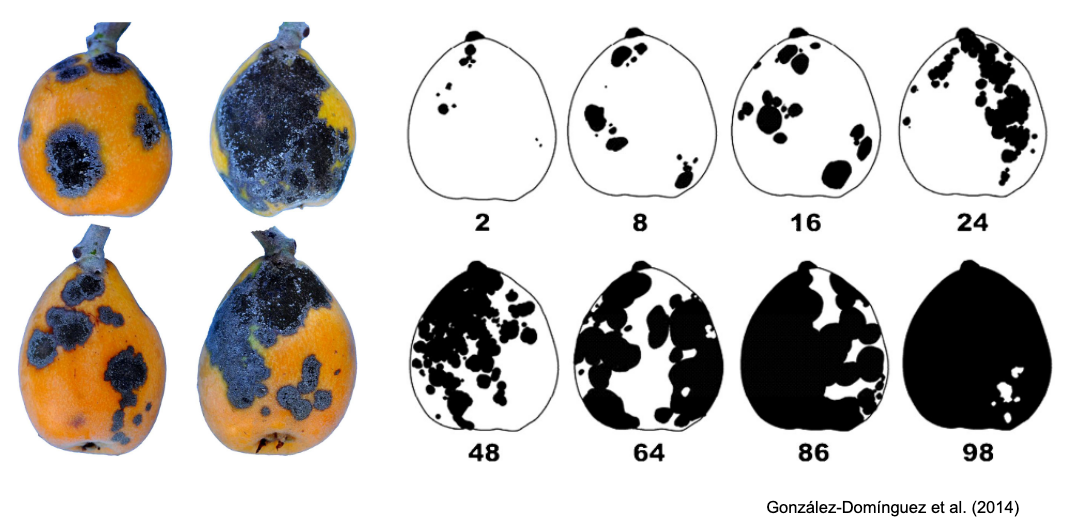
\includegraphics[width=6.51042in,height=\textheight]{imgs/sad-loquat.png}

}

\caption{\label{fig-sad-loquat}Actual photos of symptoms of loquat scab
on fruit (left) and a SADs with eight diagrams (right). Each number
represents severity as the percent area affected (González-Domínguez et
al. 2014)}

\end{figure}

\begin{center}\rule{0.5\linewidth}{0.5pt}\end{center}

\begin{figure}

{\centering 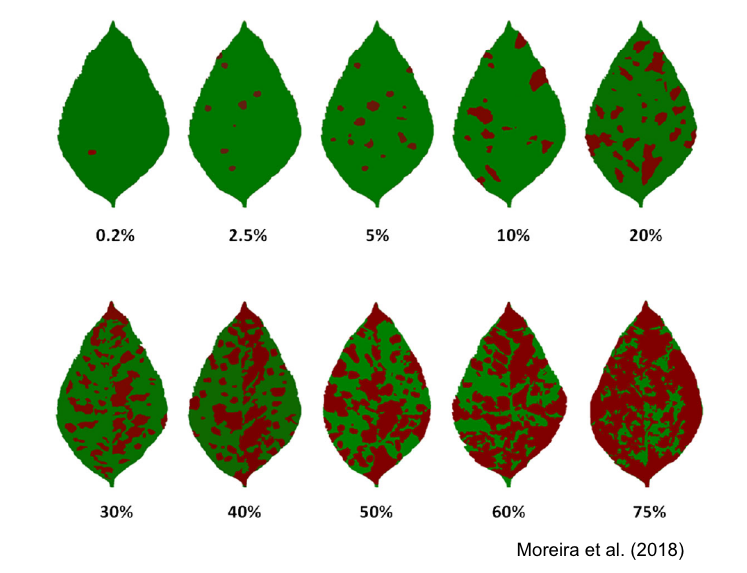
\includegraphics[width=6.47917in,height=\textheight]{imgs/sad-apple.png}

}

\caption{\label{fig-sad-apple}SADs for Glomerella leaf spot on apple
leaf. Each number represents severity as the percent area affected
(Moreira et al. 2018)}

\end{figure}

\begin{center}\rule{0.5\linewidth}{0.5pt}\end{center}

\begin{figure}

{\centering 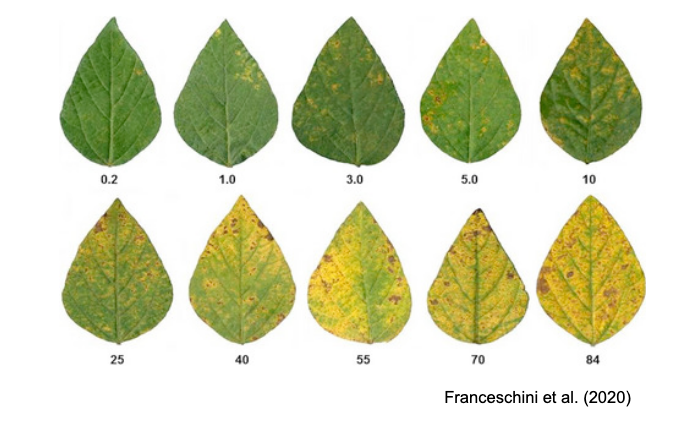
\includegraphics[width=6.51042in,height=\textheight]{imgs/sad-sbr.png}

}

\caption{\label{fig-sad-sbr}SADs for soybean rust. Each number
represents severity as the percent area affected (Franceschi et al.
2020)}

\end{figure}

More SADs can be found in the
\href{https://emdelponte.github.io/sadbank/}{SADBank}, a curated
collection of articles on SAD development and validation. Click on the
image below to get access to the database.

\begin{figure}

{\centering 

\href{https://emdelponte.github.io/sadbank/}{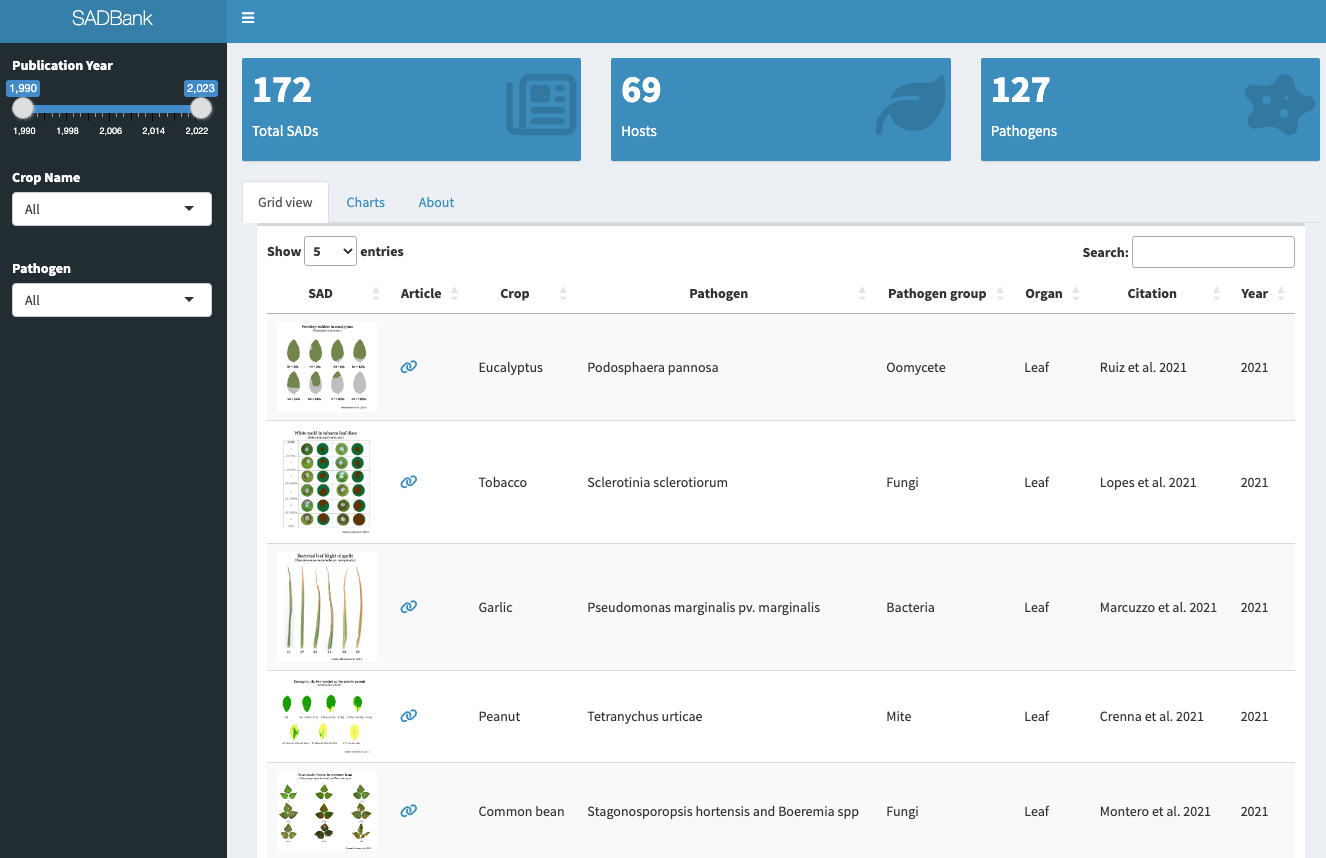
\includegraphics[width=0.87\textwidth,height=\textheight]{imgs/sadbank.png}}

}

\caption{\label{fig-sadbank}SADBank, a curated collection of articles}

\end{figure}

\hypertarget{sad-development-and-validation}{%
\section{SAD development and
validation}\label{sad-development-and-validation}}

A systematic review of the literature on SADs highlighted the most
important aspects related with the development and validation of the
tool (Del Ponte et al. 2017). A list of best practices was proposed in
the review to guide future research in the area. Follows the most
important aspects to be noted:

\begin{tcolorbox}[enhanced jigsaw, titlerule=0mm, rightrule=.15mm, colbacktitle=quarto-callout-tip-color!10!white, opacitybacktitle=0.6, toptitle=1mm, leftrule=.75mm, colback=white, colframe=quarto-callout-tip-color-frame, bottomrule=.15mm, toprule=.15mm, breakable, bottomtitle=1mm, coltitle=black, title=\textcolor{quarto-callout-tip-color}{\faLightbulb}\hspace{0.5em}{Best practices on SADs development}, arc=.35mm, opacityback=0, left=2mm]

\begin{itemize}
\item
  Sample a minimum number (e.g., n = 100) of specimens from natural
  epidemics representing the range of disease severity and typical
  symptoms observed.
\item
  Use reliable image analysis software to discriminate disease symptoms
  from healthy areas to calculate percent area affected.
\item
  When designing the illustrations for the SAD set, ensure that the
  individual diagrams are prepared realistically, whether line drawn,
  actual photos, or computer generated.
\item
  The number of diagrams should be no less than 6 and no more than 10,
  distributed approximately linearly, and spaced no more than 15\%
  apart. Additional diagrams (±2) should be included between 0 and 10\%
  severity.
\item
  For the validation trial, select at least 50 specimens representing
  the full range of actual severity and symptom patterns.
\item
  When selecting raters (a minimum of 15) for validation, make sure they
  do not have previous experience in using the SAD under evaluation.
\item
  Provide standard instructions on how to recognize the symptoms of the
  disease and how to assess severity, first without and then with the
  SAD.
\item
  Ideally repeat the assessment in time, with a 1- or 2-week interval,
  both without and with the aid, using the same set of raters in order
  to evaluate the effect of training and experience on gains in
  accuracy.
\item
  Both pre- and posttest experiment conditions should be the same to
  avoid any impact of distraction on accuracy of estimates during the
  tests.
\end{itemize}

\end{tcolorbox}

\hypertarget{designing-sads-in-r}{%
\section{Designing SADs in R}\label{designing-sads-in-r}}

The diagrams used in a set have been developed using various methods and
technologies, ranging from hand-drawn diagrams to actual photographs
(Del Ponte et al. 2017). There is an increasing trend towards using
actual photos that are digitally analyzed using standard image analysis
software to determine the percent area affected. With this approach, a
large set of images is analyzed, and some images are chosen to represent
the severities in the SAD according to the scale structure.

In R, the pliman package has a function called \texttt{sad()} which
allows the automatic generation of a SADs with a pre-defined number of
diagrams. Firstly, as shown in the
\href{data-actual-severity.html}{previous chapter}, the set of images to
be selected needs to be analysed using the \texttt{measure\_disease()}
function. Then, a SADs is automatically generated. In the function, the
specimens with the smallest and highest severity will be selected for
the SAD. The intermediate diagrams are sampled sequentially to achieve
the pre-defined number of images after the severity has been ordered
from low to high. More details of the function
\href{https://tiagoolivoto.github.io/pliman/reference/sad.html}{here}.

Let's use the \protect\hyperlink{multiple-images}{same set} of 10
soybean leaves, as seen in the previous chapter, depicting the rust
symptoms and create the \texttt{sbr} object.

\begin{Shaded}
\begin{Highlighting}[]
\FunctionTok{library}\NormalTok{(pliman)}
\NormalTok{h }\OtherTok{\textless{}{-}} \FunctionTok{image\_import}\NormalTok{(}\StringTok{"imgs/sbr\_h.png"}\NormalTok{)}
\NormalTok{s }\OtherTok{\textless{}{-}} \FunctionTok{image\_import}\NormalTok{(}\StringTok{"imgs/sbr\_s.png"}\NormalTok{)}
\NormalTok{b }\OtherTok{\textless{}{-}} \FunctionTok{image\_import}\NormalTok{(}\StringTok{"imgs/sbr\_b.png"}\NormalTok{)}

\NormalTok{sbr }\OtherTok{\textless{}{-}} \FunctionTok{measure\_disease}\NormalTok{(}
  \AttributeTok{pattern =} \StringTok{"img"}\NormalTok{,}
  \AttributeTok{dir\_original =} \StringTok{"imgs/originals"}\NormalTok{ ,}
  \AttributeTok{dir\_processed =} \StringTok{"imgs/processed"}\NormalTok{,}
  \AttributeTok{save\_image =} \ConstantTok{TRUE}\NormalTok{,}
  \AttributeTok{img\_healthy =}\NormalTok{ h,}
  \AttributeTok{img\_symptoms =}\NormalTok{ s,}
  \AttributeTok{img\_background =}\NormalTok{ b,}
  \AttributeTok{show\_original =} \ConstantTok{FALSE}\NormalTok{, }\CommentTok{\# set to TRUE for showing the original.}
  \AttributeTok{col\_background =} \StringTok{"white"}\NormalTok{, }
  \AttributeTok{verbose =} \ConstantTok{FALSE}\NormalTok{,}
  \AttributeTok{plot =} \ConstantTok{FALSE}
\NormalTok{)}
\end{Highlighting}
\end{Shaded}

We are ready to run the \texttt{sad()} function to create a SADs with
five diagrams side by side. The resulting SADs is in two-color as
standard. Set the argument \texttt{show\_original} to \texttt{TRUE} for
showing the orignal image in the SADs.

\begin{Shaded}
\begin{Highlighting}[]
\FunctionTok{sad}\NormalTok{(sbr, }\DecValTok{5}\NormalTok{, }\AttributeTok{ncol =} \DecValTok{5}\NormalTok{)}
\end{Highlighting}
\end{Shaded}

\includegraphics{data-sads_files/figure-latex/unnamed-chunk-2-1.pdf}

\hypertarget{analysis-of-sads-validation-data}{%
\section{Analysis of SADs validation
data}\label{analysis-of-sads-validation-data}}

To evaluate the effect of SAD on accuracy components, analyze the data,
preferably using concordance analysis methods
(\href{data-accuracy.html}{see chapter}), to fully explore which
component is affected and to gain insight into the ramification of
errors. Linear regression should not be used as the sole method but it
could be complementary for comparison with previous literature.

Inferential methods should be used for testing hypotheses related to
gain in accuracy. If parametric tests are used (paired t-test for
example), make sure to check that the assumptions are not violated.
Alternatively, nonparametric tests (Wilcoxon signed rank) or
nonparametric bootstrapping should be used when the conditions for
parametric tests are not met. More recently, a (parametric) mixed
modelling framework has been used to analyse SADs validation data where
raters are taken as a random effects in the model (González-Domínguez et
al. 2014; Franceschi et al. 2020; Pereira et al. 2020).

\hypertarget{non-parametric-boostrapping-of-differences}{%
\subsection{Non parametric boostrapping of
differences}\label{non-parametric-boostrapping-of-differences}}

Bootstrap is a resampling method where large numbers of samples of the
same size are repeatedly drawn, \textbf{\emph{with replacement}}, from a
single original sample. It is commonly used when the distribution of a
statistic is unknown or complicated and the sample size is too small to
draw a valid inference.

A bootstrap-based equivalence test procedure was first proposed as
complementary to parametric (paired t-test) or non-parametric (Wilcoxon)
to analyze severity estimation data in a study on the development and
validation of a SADs for pecan scab (Yadav et al. 2012). The equivalence
test was used to calculate 95\% confidence intervals for each statistic
by bootstrapping using the percentile method (with an equivalence test,
the null hypothesis is the converse of H0, i.e.~the null hypothesis is
non-equivalence). In that study, the test was used to compare means of
the CCC statistics across raters under two conditions: 1) without versus
with the SAD; and 2) experienced versus inexperienced raters.

To apply the bootstrap-based equivalence test, let's work with the CCC
data for a sample of 20 raters who estimated severity of soybean rust
SAD first without and then with the aid. The CCC was calculated as shown
\protect\hyperlink{concordance-correlation-coefficient}{here}.

\begin{Shaded}
\begin{Highlighting}[]
\FunctionTok{library}\NormalTok{(tidyverse)}
\FunctionTok{library}\NormalTok{(r4pde)}

\NormalTok{sbr }\OtherTok{\textless{}{-}}\NormalTok{ tibble}\SpecialCharTok{::}\FunctionTok{tribble}\NormalTok{(}
  \SpecialCharTok{\textasciitilde{}}\NormalTok{rater, }\SpecialCharTok{\textasciitilde{}}\NormalTok{aided, }\SpecialCharTok{\textasciitilde{}}\NormalTok{unaided,}
      \DecValTok{1}\NormalTok{,   }\FloatTok{0.97}\NormalTok{,     }\FloatTok{0.85}\NormalTok{,}
      \DecValTok{2}\NormalTok{,   }\FloatTok{0.97}\NormalTok{,     }\FloatTok{0.85}\NormalTok{,}
      \DecValTok{3}\NormalTok{,   }\FloatTok{0.95}\NormalTok{,     }\FloatTok{0.82}\NormalTok{,}
      \DecValTok{4}\NormalTok{,   }\FloatTok{0.93}\NormalTok{,     }\FloatTok{0.69}\NormalTok{,}
      \DecValTok{5}\NormalTok{,   }\FloatTok{0.97}\NormalTok{,     }\FloatTok{0.84}\NormalTok{,}
      \DecValTok{6}\NormalTok{,   }\FloatTok{0.96}\NormalTok{,     }\FloatTok{0.86}\NormalTok{,}
      \DecValTok{7}\NormalTok{,   }\FloatTok{0.98}\NormalTok{,     }\FloatTok{0.78}\NormalTok{,}
      \DecValTok{8}\NormalTok{,   }\FloatTok{0.93}\NormalTok{,     }\FloatTok{0.72}\NormalTok{,}
      \DecValTok{9}\NormalTok{,   }\FloatTok{0.94}\NormalTok{,     }\FloatTok{0.67}\NormalTok{,}
     \DecValTok{10}\NormalTok{,   }\FloatTok{0.95}\NormalTok{,     }\FloatTok{0.53}\NormalTok{,}
     \DecValTok{11}\NormalTok{,   }\FloatTok{0.94}\NormalTok{,     }\FloatTok{0.78}\NormalTok{,}
     \DecValTok{12}\NormalTok{,   }\FloatTok{0.98}\NormalTok{,     }\FloatTok{0.89}\NormalTok{,}
     \DecValTok{13}\NormalTok{,   }\FloatTok{0.96}\NormalTok{,      }\FloatTok{0.8}\NormalTok{,}
     \DecValTok{14}\NormalTok{,   }\FloatTok{0.98}\NormalTok{,     }\FloatTok{0.87}\NormalTok{,}
     \DecValTok{15}\NormalTok{,   }\FloatTok{0.98}\NormalTok{,      }\FloatTok{0.9}\NormalTok{,}
     \DecValTok{16}\NormalTok{,   }\FloatTok{0.98}\NormalTok{,     }\FloatTok{0.87}\NormalTok{,}
     \DecValTok{17}\NormalTok{,   }\FloatTok{0.98}\NormalTok{,     }\FloatTok{0.84}\NormalTok{,}
     \DecValTok{18}\NormalTok{,   }\FloatTok{0.97}\NormalTok{,     }\FloatTok{0.86}\NormalTok{,}
     \DecValTok{19}\NormalTok{,   }\FloatTok{0.98}\NormalTok{,     }\FloatTok{0.89}\NormalTok{,}
     \DecValTok{20}\NormalTok{,   }\FloatTok{0.98}\NormalTok{,     }\FloatTok{0.78}
\NormalTok{  )}
\end{Highlighting}
\end{Shaded}

Let's visualize the data using boxplots. Each point in the plot
represents a rater.

\begin{Shaded}
\begin{Highlighting}[]
\FunctionTok{theme\_set}\NormalTok{(}\FunctionTok{theme\_r4pde}\NormalTok{())}
\NormalTok{sbr }\SpecialCharTok{|\textgreater{}} 
  \FunctionTok{pivot\_longer}\NormalTok{(}\DecValTok{2}\SpecialCharTok{:}\DecValTok{3}\NormalTok{, }\AttributeTok{names\_to =} \StringTok{"condition"}\NormalTok{, }\AttributeTok{values\_to =}\StringTok{"estimate"}\NormalTok{) }\SpecialCharTok{|\textgreater{}} 
  \FunctionTok{ggplot}\NormalTok{(}\FunctionTok{aes}\NormalTok{(condition, estimate))}\SpecialCharTok{+}
  \FunctionTok{geom\_boxplot}\NormalTok{(}\AttributeTok{outlier.colour =} \ConstantTok{NA}\NormalTok{)}\SpecialCharTok{+}
  \FunctionTok{geom\_jitter}\NormalTok{(}\AttributeTok{width =} \FloatTok{0.05}\NormalTok{, }\AttributeTok{size =} \DecValTok{2}\NormalTok{, }\AttributeTok{alpha =} \FloatTok{0.5}\NormalTok{)}\SpecialCharTok{+}
  \FunctionTok{theme\_r4pde}\NormalTok{()}\SpecialCharTok{+}
  \FunctionTok{ylim}\NormalTok{(}\FloatTok{0.4}\NormalTok{,}\DecValTok{1}\NormalTok{)}
\end{Highlighting}
\end{Shaded}

\includegraphics{data-sads_files/figure-latex/unnamed-chunk-4-1.pdf}

To proceed with bootstrapping, we first create a new variable to hold
the differences between the means of the estimates (aided minus
unaided). If the 95\% CI does not include zero, this means that there
was a significant improvement in the statistics.

\begin{Shaded}
\begin{Highlighting}[]
\CommentTok{\# diff of means}
\NormalTok{sbr}\SpecialCharTok{$}\NormalTok{diff }\OtherTok{\textless{}{-}}\NormalTok{ sbr}\SpecialCharTok{$}\NormalTok{aided }\SpecialCharTok{{-}}\NormalTok{ sbr}\SpecialCharTok{$}\NormalTok{unaided}

\NormalTok{sbr }\SpecialCharTok{|\textgreater{}} 
  \FunctionTok{ggplot}\NormalTok{(}\FunctionTok{aes}\NormalTok{(}\AttributeTok{x=}\NormalTok{ diff))}\SpecialCharTok{+}
  \FunctionTok{theme\_r4pde}\NormalTok{()}\SpecialCharTok{+}
  \FunctionTok{geom\_histogram}\NormalTok{(}\AttributeTok{bins =} \DecValTok{10}\NormalTok{, }\AttributeTok{color =} \StringTok{"white"}\NormalTok{)}
\end{Highlighting}
\end{Shaded}

\includegraphics{data-sads_files/figure-latex/unnamed-chunk-5-1.pdf}

Using the simpleboot and boot packages of R:

\begin{Shaded}
\begin{Highlighting}[]
\FunctionTok{library}\NormalTok{(simpleboot)}
\end{Highlighting}
\end{Shaded}

\begin{verbatim}
Simple Bootstrap Routines (1.1-7)
\end{verbatim}

\begin{Shaded}
\begin{Highlighting}[]
\NormalTok{b.mean }\OtherTok{\textless{}{-}} \FunctionTok{one.boot}\NormalTok{(sbr}\SpecialCharTok{$}\NormalTok{diff, mean, }\DecValTok{999}\NormalTok{)}
\NormalTok{boot}\SpecialCharTok{::}\FunctionTok{boot.ci}\NormalTok{(b.mean)}
\end{Highlighting}
\end{Shaded}

\begin{verbatim}
Warning in boot::boot.ci(b.mean): bootstrap variances needed for studentized
intervals
\end{verbatim}

\begin{verbatim}
BOOTSTRAP CONFIDENCE INTERVAL CALCULATIONS
Based on 999 bootstrap replicates

CALL : 
boot::boot.ci(boot.out = b.mean)

Intervals : 
Level      Normal              Basic         
95%   ( 0.1261,  0.1946 )   ( 0.1230,  0.1910 )  

Level     Percentile            BCa          
95%   ( 0.1280,  0.1960 )   ( 0.1295,  0.2000 )  
Calculations and Intervals on Original Scale
\end{verbatim}

\begin{Shaded}
\begin{Highlighting}[]
\FunctionTok{mean}\NormalTok{(b.mean}\SpecialCharTok{$}\NormalTok{data)}
\end{Highlighting}
\end{Shaded}

\begin{verbatim}
[1] 0.1595
\end{verbatim}

\begin{Shaded}
\begin{Highlighting}[]
\FunctionTok{hist}\NormalTok{(b.mean)}
\end{Highlighting}
\end{Shaded}

\includegraphics{data-sads_files/figure-latex/unnamed-chunk-6-1.pdf}

Using the bootstrap package:

\begin{Shaded}
\begin{Highlighting}[]
\FunctionTok{library}\NormalTok{(bootstrap)}
\NormalTok{b }\OtherTok{\textless{}{-}} \FunctionTok{bootstrap}\NormalTok{(sbr}\SpecialCharTok{$}\NormalTok{diff, }\DecValTok{999}\NormalTok{, mean)}
\FunctionTok{quantile}\NormalTok{(b}\SpecialCharTok{$}\NormalTok{thetastar, }\FunctionTok{c}\NormalTok{(.}\DecValTok{025}\NormalTok{,.}\DecValTok{975}\NormalTok{))}
\end{Highlighting}
\end{Shaded}

\begin{verbatim}
 2.5% 97.5% 
0.128 0.195 
\end{verbatim}

\begin{Shaded}
\begin{Highlighting}[]
\FunctionTok{mean}\NormalTok{(b}\SpecialCharTok{$}\NormalTok{thetastar)}
\end{Highlighting}
\end{Shaded}

\begin{verbatim}
[1] 0.1577758
\end{verbatim}

\begin{Shaded}
\begin{Highlighting}[]
\FunctionTok{sd}\NormalTok{(b}\SpecialCharTok{$}\NormalTok{thetastar)}
\end{Highlighting}
\end{Shaded}

\begin{verbatim}
[1] 0.01731425
\end{verbatim}

\begin{Shaded}
\begin{Highlighting}[]
\NormalTok{se }\OtherTok{\textless{}{-}} \ControlFlowTok{function}\NormalTok{(x) }\FunctionTok{sqrt}\NormalTok{(}\FunctionTok{var}\NormalTok{(x)}\SpecialCharTok{/}\FunctionTok{length}\NormalTok{(x))}
\FunctionTok{se}\NormalTok{(b}\SpecialCharTok{$}\NormalTok{thetastar)}
\end{Highlighting}
\end{Shaded}

\begin{verbatim}
[1] 0.0005477987
\end{verbatim}

Both procedures shown above have led to similar results. The 95\% CIs of
the differences did not include zero, so a significant improvement in
accuracy can be inferred.

\hypertarget{parametric-and-non-parametric-paired-sample-tests}{%
\subsection{Parametric and non-parametric paired sample
tests}\label{parametric-and-non-parametric-paired-sample-tests}}

When two estimates are gathered from the same rater at different times,
these data points are not independent. In such situations, a
\textbf{paired sample t-test} can be utilized to test if the mean
difference between two sets of observations is zero. This test requires
each subject (or leaf, in our context) to be measured or estimated
twice, resulting in \emph{pairs} of observations. However, if the
assumptions of the test (such as normality) are violated, a
non-parametric equivalent, such as the Wilcoxon signed-rank test, also
known as the \textbf{Wilcoxon test}, can be employed. This alternative
is particularly useful when the data are not normally distributed.

To proceed with these tests, we first need to ascertain whether our data
are normally distributed. We should also verify whether the variances
are equal. Let's now apply these two tests to our data and compare the
results.

\begin{Shaded}
\begin{Highlighting}[]
\CommentTok{\# normality test}
\FunctionTok{shapiro.test}\NormalTok{(sbr}\SpecialCharTok{$}\NormalTok{aided)}
\end{Highlighting}
\end{Shaded}

\begin{verbatim}

    Shapiro-Wilk normality test

data:  sbr$aided
W = 0.82529, p-value = 0.002111
\end{verbatim}

\begin{Shaded}
\begin{Highlighting}[]
\FunctionTok{shapiro.test}\NormalTok{(sbr}\SpecialCharTok{$}\NormalTok{unaided)}
\end{Highlighting}
\end{Shaded}

\begin{verbatim}

    Shapiro-Wilk normality test

data:  sbr$unaided
W = 0.83769, p-value = 0.003338
\end{verbatim}

\begin{Shaded}
\begin{Highlighting}[]
\CommentTok{\# equal variance test}
\FunctionTok{var.test}\NormalTok{(sbr}\SpecialCharTok{$}\NormalTok{aided, sbr}\SpecialCharTok{$}\NormalTok{unaided)}
\end{Highlighting}
\end{Shaded}

\begin{verbatim}

    F test to compare two variances

data:  sbr$aided and sbr$unaided
F = 0.037789, num df = 19, denom df = 19, p-value = 1.53e-09
alternative hypothesis: true ratio of variances is not equal to 1
95 percent confidence interval:
 0.01495720 0.09547109
sample estimates:
ratio of variances 
        0.03778862 
\end{verbatim}

\begin{Shaded}
\begin{Highlighting}[]
\CommentTok{\# paired t{-}test}
\FunctionTok{t.test}\NormalTok{(sbr}\SpecialCharTok{$}\NormalTok{aided, sbr}\SpecialCharTok{$}\NormalTok{unaided, }\AttributeTok{paired =} \ConstantTok{TRUE}\NormalTok{)}
\end{Highlighting}
\end{Shaded}

\begin{verbatim}

    Paired t-test

data:  sbr$aided and sbr$unaided
t = 8.812, df = 19, p-value = 3.873e-08
alternative hypothesis: true difference in means is not equal to 0
95 percent confidence interval:
 0.1216158 0.1973842
sample estimates:
mean of the differences 
                 0.1595 
\end{verbatim}

\begin{Shaded}
\begin{Highlighting}[]
\CommentTok{\# Wilcoxon test}
\FunctionTok{wilcox.test}\NormalTok{(sbr}\SpecialCharTok{$}\NormalTok{aided, sbr}\SpecialCharTok{$}\NormalTok{unaided, }\AttributeTok{paired =} \ConstantTok{TRUE}\NormalTok{)}
\end{Highlighting}
\end{Shaded}

\begin{verbatim}
Warning in wilcox.test.default(sbr$aided, sbr$unaided, paired = TRUE): cannot
compute exact p-value with ties
\end{verbatim}

\begin{verbatim}

    Wilcoxon signed rank test with continuity correction

data:  sbr$aided and sbr$unaided
V = 210, p-value = 9.449e-05
alternative hypothesis: true location shift is not equal to 0
\end{verbatim}

As shown above, the two assumptions were violated, so we could rely more
confidently on the non-parametric test.

\hypertarget{mixed-effects-modeling}{%
\subsection{Mixed effects modeling}\label{mixed-effects-modeling}}

Mixed models, also known as mixed effects models or multilevel models,
are an extension of traditional linear models that are used for
analyzing hierarchical or clustered data. These models are particularly
useful when dealing with data where observations may not be fully
independent, or when the assumption of independence is violated. This
happens, for instance, when data are collected over time from the same
individuals or units, or when individuals are grouped or nested within
higher-level units, such as in our case where measurements are taken by
different raters (Brown 2021).

Mixed models enable us to model both fixed and random effects. Fixed
effects represent the usual regression parameters that we are primarily
interested in estimating, while random effects model the random
variation that occurs at different levels of hierarchy or clustering.
They allow us to account for variability among different levels of data,
like inter-rater variability or intra-subject variability in repeated
measures designs.

In our context, we consider raters as random effects because we view
them as a sample drawn from a larger population of potential raters, and
our goal is to generalize our findings to this larger population. If we
were to sample additional raters, we would expect these new raters to
differ from our current ones. However, by considering raters as a random
effect in our model, we can account for this inter-rater variability and
make more accurate inferences about the overall population.

The random effects component in the mixed model allows us to capture and
model the additional variance that is not explicitly accounted for by
the fixed effects in our model. In other words, random effects help us
to capture and quantify the `unexplained' or `residual' variation that
exists within and between the clusters or groups in our data. This could
include, for instance, variation in disease measurements that are taken
repeatedly from the same subjects. In conclusion, mixed models provide a
robust and flexible framework for modeling hierarchical or clustered
data, allowing us to effectively account for both fixed and random
effects and to make more accurate inferences about our data.

Let's start reshaping our data to the long format and assign them to a
new data frame.

\begin{Shaded}
\begin{Highlighting}[]
\NormalTok{sbr2 }\OtherTok{\textless{}{-}}\NormalTok{ sbr }\SpecialCharTok{|\textgreater{}} 
  \FunctionTok{pivot\_longer}\NormalTok{(}\DecValTok{2}\SpecialCharTok{:}\DecValTok{3}\NormalTok{, }\AttributeTok{names\_to =} \StringTok{"condition"}\NormalTok{, }\AttributeTok{values\_to =} \StringTok{"estimate"}\NormalTok{)}
\end{Highlighting}
\end{Shaded}

Now we fit the mixed model using the \texttt{lmer} function of the
\emph{lme4} package. We will fit the model to the logit of the estimate
because they should be bounded between zero and one. Preliminary
analysis using non-transformed or log-transformed data resulted in lack
of normality of residuals and heterocedasticity (not shown).

\begin{Shaded}
\begin{Highlighting}[]
\FunctionTok{library}\NormalTok{(lme4) }
\FunctionTok{library}\NormalTok{(car) }\CommentTok{\# for logit function}
\NormalTok{mix }\OtherTok{\textless{}{-}} \FunctionTok{lmer}\NormalTok{(}\FunctionTok{logit}\NormalTok{(estimate) }\SpecialCharTok{\textasciitilde{}}\NormalTok{ condition }\SpecialCharTok{+}\NormalTok{ (}\DecValTok{1} \SpecialCharTok{|}\NormalTok{ rater), }\AttributeTok{data =}\NormalTok{ sbr2)}

\CommentTok{\# Check model performance}
\FunctionTok{library}\NormalTok{(performance)}
\FunctionTok{check\_normality}\NormalTok{(mix)}
\end{Highlighting}
\end{Shaded}

\begin{verbatim}
OK: residuals appear as normally distributed (p = 0.381).
\end{verbatim}

\begin{Shaded}
\begin{Highlighting}[]
\FunctionTok{check\_heteroscedasticity}\NormalTok{(mix)}
\end{Highlighting}
\end{Shaded}

\begin{verbatim}
OK: Error variance appears to be homoscedastic (p = 0.961).
\end{verbatim}

\begin{Shaded}
\begin{Highlighting}[]
\CommentTok{\# Check effect of condition}
\NormalTok{car}\SpecialCharTok{::}\FunctionTok{Anova}\NormalTok{(mix)}
\end{Highlighting}
\end{Shaded}

\begin{verbatim}
Analysis of Deviance Table (Type II Wald chisquare tests)

Response: logit(estimate)
           Chisq Df Pr(>Chisq)    
condition 458.44  1  < 2.2e-16 ***
---
Signif. codes:  0 '***' 0.001 '**' 0.01 '*' 0.05 '.' 0.1 ' ' 1
\end{verbatim}

\begin{Shaded}
\begin{Highlighting}[]
\CommentTok{\# Estimate the means for each group}
\FunctionTok{library}\NormalTok{(emmeans)}
\NormalTok{em }\OtherTok{\textless{}{-}} \FunctionTok{emmeans}\NormalTok{(mix, }\SpecialCharTok{\textasciitilde{}}\NormalTok{ condition, }\AttributeTok{transform =} \StringTok{"response"}\NormalTok{)}
\NormalTok{em}
\end{Highlighting}
\end{Shaded}

\begin{verbatim}
 condition response      SE   df lower.CL upper.CL
 aided        0.968 0.00359 25.5    0.960    0.975
 unaided      0.817 0.01719 25.5    0.781    0.852

Degrees-of-freedom method: inherited from kenward-roger when re-gridding 
Confidence level used: 0.95 
\end{verbatim}

\begin{Shaded}
\begin{Highlighting}[]
\CommentTok{\# Contrast the means}
\FunctionTok{pairs}\NormalTok{(em)}
\end{Highlighting}
\end{Shaded}

\begin{verbatim}
 contrast        estimate     SE   df t.ratio p.value
 aided - unaided    0.151 0.0149 25.5  10.141  <.0001

Degrees-of-freedom method: inherited from kenward-roger when re-gridding 
\end{verbatim}

\begin{Shaded}
\begin{Highlighting}[]
\CommentTok{\# plot the means with 95\% CIs}
\FunctionTok{plot}\NormalTok{(em) }\SpecialCharTok{+}
  \FunctionTok{coord\_flip}\NormalTok{()}\SpecialCharTok{+}
  \FunctionTok{xlim}\NormalTok{(}\FloatTok{0.7}\NormalTok{,}\DecValTok{1}\NormalTok{)}\SpecialCharTok{+}
  \FunctionTok{theme\_r4pde}\NormalTok{()}
\end{Highlighting}
\end{Shaded}

\includegraphics{data-sads_files/figure-latex/unnamed-chunk-10-1.pdf}

As shown above, we can reject the null hypothesis that the means are the
same between the two groups.

Alternatively, we could fit GLMMs - generalized linear mixed models,
which extend the traditional linear mixed models to accommodate response
variables that follow different distributions. They are particularly
useful when the response variable does not follow a normal distribution
and cannot be adequately transformed to meet the parametric assumptions
of traditional linear models. The glmmTMB package in R provides a
convenient and flexible platform to fit GLMMs using a variety of
distributions (Brooks et al. 2017).

In our case, considering our response variable bounded between 0 and 1,
a Beta distribution might be a suitable choice. Beta distribution is a
continuous probability distribution defined on the interval {[}0, 1{]},
and is commonly used for modelling variables that represent proportions
or percentages.

The function \texttt{glmmTMB()} from the \emph{glmmTMB} package can be
used to fit a GLMM with a Beta distribution. In this function, we
specify the distribution family as \texttt{beta\_family()}.

\begin{Shaded}
\begin{Highlighting}[]
\FunctionTok{library}\NormalTok{(glmmTMB)}
\NormalTok{mix2 }\OtherTok{\textless{}{-}}  \FunctionTok{glmmTMB}\NormalTok{(estimate }\SpecialCharTok{\textasciitilde{}}\NormalTok{ condition }\SpecialCharTok{+}\NormalTok{ (}\DecValTok{1}\SpecialCharTok{|}\NormalTok{ rater), }
                 \AttributeTok{data =}\NormalTok{ sbr2, }
                 \AttributeTok{family =} \FunctionTok{beta\_family}\NormalTok{())}
\end{Highlighting}
\end{Shaded}

Because the package \emph{performance} does not handle the
\emph{glmmTMB} output, we will use the \emph{DHARMa} package in R which
can be particularly useful for checking the assumptions of your GLMM
fitted with \texttt{glmmTMB()}. The package provides a convenient way to
carry out residual diagnostics for models fitted via maximum likelihood
estimation, including GLMMs. This package creates standardized residuals
from the observed responses and the predicted responses of a fitted
model, and then compares these residuals to a simulated set of residuals
under a correct model.

\begin{Shaded}
\begin{Highlighting}[]
\FunctionTok{library}\NormalTok{(DHARMa)}

\FunctionTok{plot}\NormalTok{(}\FunctionTok{simulateResiduals}\NormalTok{(mix2))}
\end{Highlighting}
\end{Shaded}

\includegraphics{data-sads_files/figure-latex/unnamed-chunk-12-1.pdf}

In this example, \texttt{simulateResiduals()} generates simulated
residuals from your fitted model, and the plot creates a plot of these
residuals. This showed that the residuals from our model are uniformly
distributed, which is an assumption of GLMMs. We can now proceed with
the posthoc analysis and noticed that the results are similar to when
the response variable was transformed to logit.

\begin{Shaded}
\begin{Highlighting}[]
\NormalTok{car}\SpecialCharTok{::}\FunctionTok{Anova}\NormalTok{(mix2)}
\end{Highlighting}
\end{Shaded}

\begin{verbatim}
Analysis of Deviance Table (Type II Wald chisquare tests)

Response: estimate
           Chisq Df Pr(>Chisq)    
condition 400.93  1  < 2.2e-16 ***
---
Signif. codes:  0 '***' 0.001 '**' 0.01 '*' 0.05 '.' 0.1 ' ' 1
\end{verbatim}

\begin{Shaded}
\begin{Highlighting}[]
\FunctionTok{library}\NormalTok{(emmeans)}
\NormalTok{em }\OtherTok{\textless{}{-}} \FunctionTok{emmeans}\NormalTok{(mix2, }\SpecialCharTok{\textasciitilde{}}\NormalTok{ condition, }\AttributeTok{transform =} \StringTok{"response"}\NormalTok{)}
\NormalTok{em}
\end{Highlighting}
\end{Shaded}

\begin{verbatim}
 condition response     SE df lower.CL upper.CL
 aided        0.967 0.0043 36    0.958    0.976
 unaided      0.814 0.0167 36    0.780    0.848

Confidence level used: 0.95 
\end{verbatim}

\begin{Shaded}
\begin{Highlighting}[]
\CommentTok{\# Contrast the means}
\FunctionTok{pairs}\NormalTok{(em)}
\end{Highlighting}
\end{Shaded}

\begin{verbatim}
 contrast        estimate     SE df t.ratio p.value
 aided - unaided    0.153 0.0139 36  11.001  <.0001
\end{verbatim}

\hypertarget{training-sessions}{%
\chapter{Training sessions}\label{training-sessions}}

\hypertarget{training-sessions-1}{%
\section{Training sessions}\label{training-sessions-1}}

In the same way that Standard Area Diagrams (SADs) can improve the
accuracy of visual estimates of disease severity, exposure to a diverse
set of diagrams or actual images with known severity values can
significantly enhance a rater's assessment proficiency. The key to this
improvement is the frequent exposure to various levels of severity,
which enables the rater to better calibrate their judgments over time.

As the rater engages with these reference diagrams or images, they
develop a mental model of the severity scale. This mental model is
continually refined through repeated exposure to a variety of severity
values. This iterative learning process allows the rater to adjust their
estimations based on the feedback from known values, thus improving
their overall accuracy and precision in disease severity estimation.

Such a process, often termed `training', is particularly beneficial in
scenarios where visual estimation is the primary tool for assessing
disease severity. Training raters using sets of reference images is an
effective strategy to enhance inter-rater reliability and consistency
over time, especially when coupled with other tools like SADs.

\hypertarget{software-1}{%
\section{Software}\label{software-1}}

Indeed, the use of computerized training sessions in assessing disease
severity has a rich history, dating back to the mid-1980s when personal
computers were first introduced. These early applications were developed
using operating systems like DOS or Windows and involved software like
AREAGRAM, DISTRAIN, DISEASE.PRO, ESTIMATE, SEVERITY.PRO, and COMBRO.
These programs utilized computerized images with specific and measured
disease severities to train raters, as outlined in the review by Bock et
al. (2021a).

The main advantage of these computerized training sessions is that they
allow raters to familiarize themselves with various disease severity
levels, thereby enhancing their performance in severity estimation. Such
training has been proven to significantly improve the accuracy and
consistency of disease severity evaluations.

However, a potential limitation of this approach is the short-lived
nature of the benefits derived from such training. The skills and
proficiency gained from these computerized training sessions may degrade
over time, necessitating regular retraining for raters to maintain their
performance level. This could be due to the fact that estimation skills,
like many other skills, require regular practice for maintenance.
Without ongoing exposure to severity scales and continued practice, the
accuracy and precision of a rater's estimates may decline.

To address this challenge, it would be beneficial to implement a
structured training regimen that includes regular retraining sessions.
This could help ensure the continued proficiency of raters in estimating
disease severity, thus maintaining the accuracy and reliability of
assessments over time. Furthermore, it would be advantageous to
investigate the optimal frequency and structure of these training
sessions to maximize their effectiveness and sustainability in the long
term.

\begin{figure}

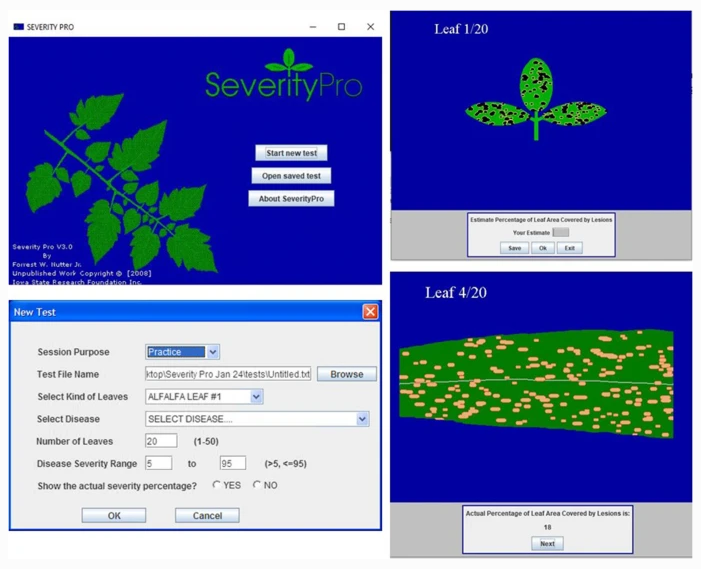
\includegraphics[width=4.28125in,height=\textheight]{imgs/severitypro.png} \hfill{}

\caption{\label{fig-severitypro}Selected screenshots from Severity.Pro,
the disease assessment training program by Forrest W. Nutter (Madden et
al. 2021).}

\end{figure}

\hypertarget{online-training-tools}{%
\subsection{Online training tools}\label{online-training-tools}}

In Brazil, the ``Sistema de treinamento de acuidade visual'' was
initially developed as a web-based system to train raters in assessing
citrus canker. The system has evolved over time and now has a current
version that is accessible on both iOS and Android platforms. You can
find the current version of the system at this
\href{http://sitav.pga.uem.br/index.php?menu=app}{link}. This platform
provides an interactive training experience to enhance the ability of
raters in accurately assessing the severity of citrus canker.

In Mexico, a specific application called \textbf{Validar-PER} has been
developed to train raters in visually assessing the severity of coffee
leaf rust. This application utilizes diagrammatic log-based scales as a
standardized approach for severity assessment. You can access the
Validar-PER application online
\href{http://royacafe.lanref.org.mx/ValidarPer/app/index.php}{here}. The
application aims to improve the proficiency of raters in evaluating the
severity of coffee leaf rust using a systematic and standardized
methodology.

\begin{figure}

\href{http://royacafe.lanref.org.mx/ValidarPer/app/index.php}{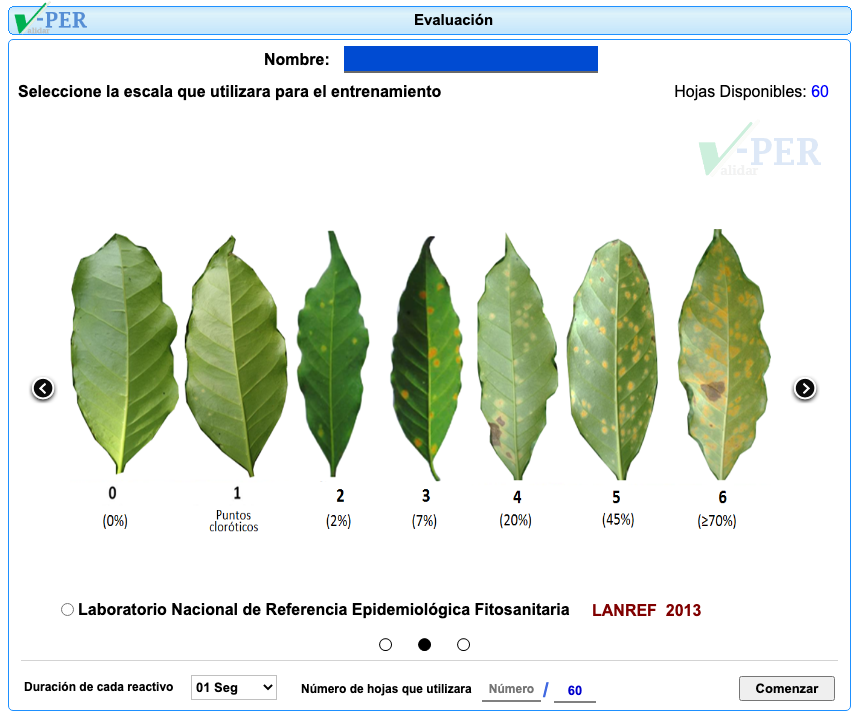
\includegraphics[width=4.47917in,height=\textheight]{imgs/validar-per.png}}

\caption{\label{fig-validar}Screen of Validar-PER, an online training
module for assessing coffee leaf rust severity}

\end{figure}

\hypertarget{training-software-made-with-r}{%
\subsection{Training software made with
R}\label{training-software-made-with-r}}

\hypertarget{trainer}{%
\subsubsection{TraineR}\label{trainer}}

\href{https://edelponte.shinyapps.io/traineR/}{TraineR}, developed by
the author of this book, is created using R and Shiny. Its purpose is to
train users in assessing disease severity, specifically expressed as the
percentage area of an organ (leaf or fruit) affected by lesions.

To use the app, users can adjust parameters for organ shape, organ
color, as well as lesion shape, lesion color, lesion number, and lesion
size. These adjustments will generate a standard area diagram with an
ellipsoidal shape.

To initiate the training, users should first set the desired number of
attempts for the session and click on the ``generate new'' button. A
diagram will then be displayed, and users should input their estimate of
the diseased area as a numeric value in percentage. The estimate will be
recorded and shown in a table along with the actual value, enabling a
comparison between the actual and estimated values.

Users can continue generating new diagrams and providing estimates until
they reach the defined number of attempts. Once the final attempt is
completed, the app will present the accuracy in the form of Lin's
concordance correlation coefficient to the user. Plots depicting the
relationship between estimates and actual values, as well as the error
of the estimates, will be displayed. Furthermore, comprehensive accuracy
statistics are also made available.

Currently, the app has certain limitations, including the inability to
overlap lesions and a maximum severity representation of approximately
60\%. Nonetheless, it remains a valuable educational and demonstration
tool.

\begin{figure}

\href{https://edelponte.shinyapps.io/traineR/}{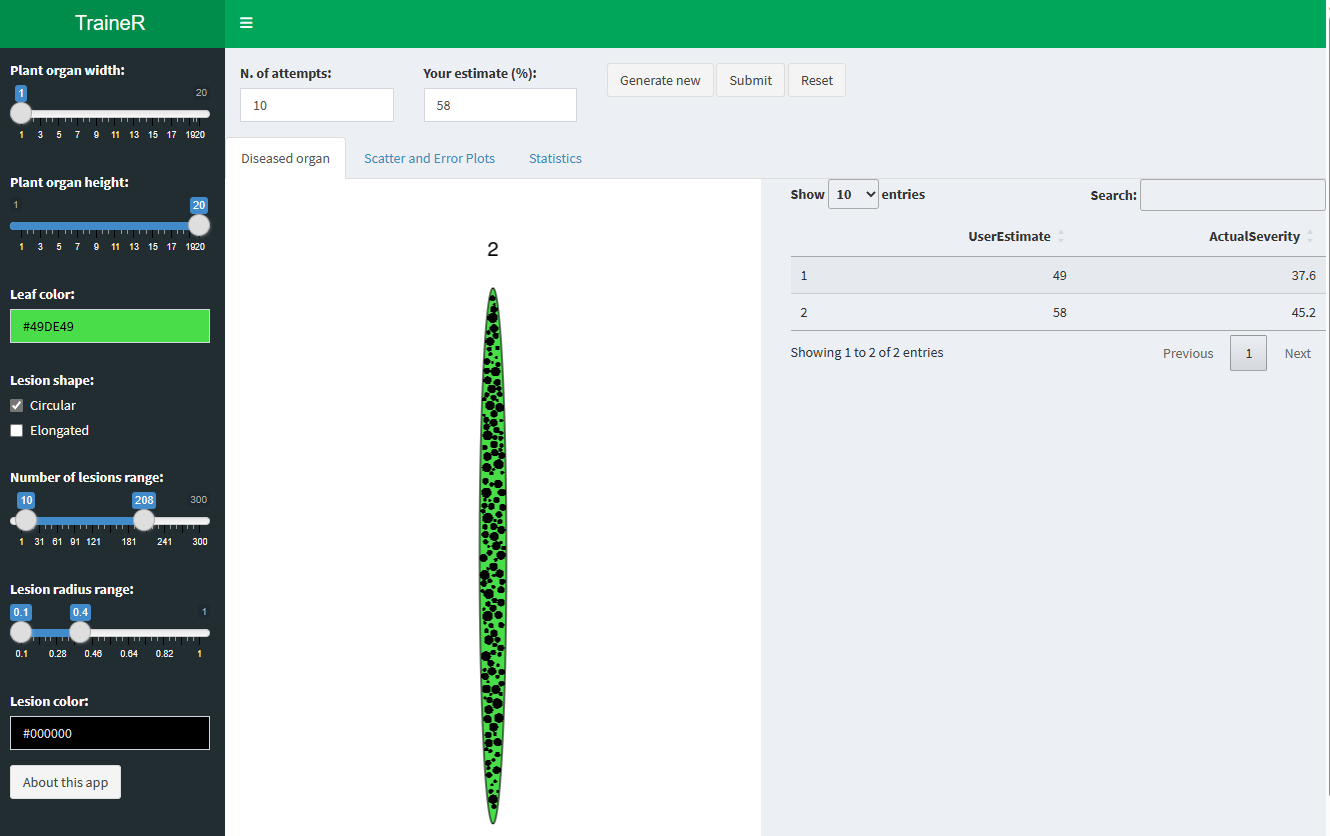
\includegraphics[width=4.47917in,height=\textheight]{imgs/trainer.png}}

\caption{\label{fig-trainer}Screen of TraineR, an online app for
training in the assessment of plant disease severity}

\end{figure}

\hypertarget{trainer2}{%
\subsubsection{Trainer2}\label{trainer2}}

\href{https://delponte.shinyapps.io/traineR2/}{Trainer2} the second
generation of TraineR, takes advantage of actual photographs showcasing
disease symptoms. This updated version allows for testing the ability of
raters to assess disease severity, particularly by evaluating the
percentage area affected based on real symptoms captured in the
photographs.

By utilizing actual images, Trainer2 offers a more realistic and
practical approach to training raters. Raters can now evaluate disease
severity by visually inspecting the symptoms depicted in the
photographs, enhancing their ability to accurately assess the extent of
damage in terms of the affected area.

The incorporation of real symptoms in Trainer2 serves as a valuable tool
for evaluating and refining the skills of raters in disease severity
assessment. It provides a more authentic training experience and helps
raters become proficient in identifying and quantifying the extent of
disease based on visual cues observed in real-life scenarios.

\begin{figure}

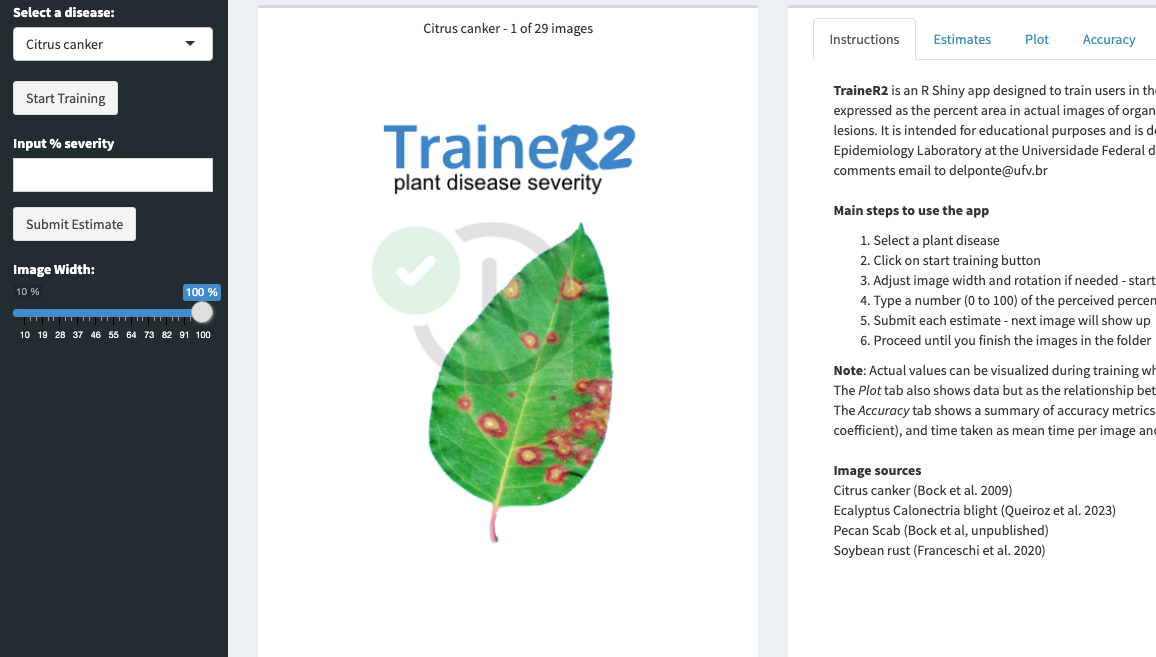
\includegraphics[width=4.47917in,height=\textheight]{imgs/trainer2.png} \hfill{}

\caption{\label{fig-trainer2}Screen of traineR2, an online for training
in the assessment of plant disease severity based on real symptoms
captured in photographs}

\end{figure}

\part{Temporal analysis}

\hypertarget{disease-progress-curves}{%
\chapter{Disease progress curves}\label{disease-progress-curves}}

\hypertarget{how-epidemics-occur}{%
\section{How epidemics occur}\label{how-epidemics-occur}}

Before knowing how epidemics develop in time, it is important to
understand how an epidemic occur. An epidemic begins when the
\textbf{primary inoculum} (a variable number of propagules able to
infect the plant) that is \emph{surviving} somewhere establishes an
intimate contact with individuals of the host population - this process
is called \emph{infection}. These inocula are usually surviving
externally to the plant host and need to \emph{disperse} (move),
passively or by means of a vector, to reach the plant. It can also be
that a growing host encounter a localized (static) source of inoculum.

Once the infection is established, the pathogen \emph{colonizes} the
plant tissues and disease symptoms are noticed. When this happens, the
\textbf{incubation period} can be measured in time units. A successful
colonization will lead to \emph{reproduction} of the pathogen inside
and/or external to the crop, and so the \textbf{latent period} is
completed, and can also be measure in time units. Finally, the
\textbf{infectious period} takes place and continues until the pathogen
is not capable of producing the \textbf{secondary inoculum} on the
infected site.

\begin{figure}

\begin{figure}[H]

\includegraphics[width=3.26in,height=4.22in]{temporal-dpc_files/figure-latex/mermaid-figure-1.png} \hfill{}

\end{figure}

\caption{\label{fig-diagram}Five main processes of the disease cycle}

\end{figure}

Epidemiologists are generally interested in determining the length of
the incubation, latent, and infectious periods as influenced by factors
related to the host, pathogen, or environment. This is relevant because
the longer it takes for the completion of the incubation and latent
periods, the lower the potential number of repeated cycles. In summary,
a single ``infection cycle'' represents all events that occur from
infection to dispersal, and this occurs only once for many diseases,
while for others there may be multiple cycles, which are defined as an
``infection chain.''

\begin{Shaded}
\begin{Highlighting}[]
\FunctionTok{library}\NormalTok{(tidyverse)}
\FunctionTok{library}\NormalTok{(r4pde)}
\NormalTok{periods }\OtherTok{\textless{}{-}}\NormalTok{ tibble}\SpecialCharTok{::}\FunctionTok{tribble}\NormalTok{(}
  \SpecialCharTok{\textasciitilde{}}\NormalTok{period, }\SpecialCharTok{\textasciitilde{}}\NormalTok{length, }\SpecialCharTok{\textasciitilde{}}\NormalTok{color, }\SpecialCharTok{\textasciitilde{}}\NormalTok{order,}
  \StringTok{"Incubation"}\NormalTok{, }\DecValTok{10}\NormalTok{, }\DecValTok{0}\NormalTok{, }\DecValTok{1}\NormalTok{,}
  \StringTok{"Latent"}\NormalTok{ , }\DecValTok{15}\NormalTok{, }\DecValTok{0}\NormalTok{, }\DecValTok{2}\NormalTok{,}
  \StringTok{"Infectious"}\NormalTok{, }\DecValTok{25}\NormalTok{, }\DecValTok{15}\NormalTok{, }\DecValTok{3}
\NormalTok{)}

\NormalTok{p }\OtherTok{\textless{}{-}}\NormalTok{ periods }\SpecialCharTok{|\textgreater{}} 
  \FunctionTok{ggplot}\NormalTok{(}\FunctionTok{aes}\NormalTok{(}\FunctionTok{reorder}\NormalTok{(period, order), length, }\AttributeTok{fill =}\NormalTok{ period))}\SpecialCharTok{+}
  \FunctionTok{geom\_col}\NormalTok{()}\SpecialCharTok{+}
  \FunctionTok{geom\_col}\NormalTok{(}\FunctionTok{aes}\NormalTok{(period, color), }\AttributeTok{color =} \StringTok{"white"}\NormalTok{, }\AttributeTok{fill =} \StringTok{"white"}\NormalTok{)}\SpecialCharTok{+}
  \FunctionTok{coord\_flip}\NormalTok{()}\SpecialCharTok{+}
  \FunctionTok{theme\_void}\NormalTok{()}\SpecialCharTok{+}
  \FunctionTok{theme}\NormalTok{(}\AttributeTok{legend.position =} \StringTok{"none"}\NormalTok{)}\SpecialCharTok{+}
  \FunctionTok{annotate}\NormalTok{(}\AttributeTok{geom =} \StringTok{"text"}\NormalTok{, }\AttributeTok{x =} \FloatTok{0.5}\NormalTok{, }\AttributeTok{y =} \DecValTok{15}\NormalTok{, }\AttributeTok{label =} \StringTok{"{-}{-}{-}{-}{-} Time {-}{-}{-}\textgreater{}"}\NormalTok{)}\SpecialCharTok{+}
  \FunctionTok{annotate}\NormalTok{(}\AttributeTok{geom =} \StringTok{"text"}\NormalTok{, }\AttributeTok{x =} \DecValTok{1}\NormalTok{, }\AttributeTok{y =} \DecValTok{5}\NormalTok{, }\AttributeTok{label =} \StringTok{"Incubation"}\NormalTok{, }\AttributeTok{color =} \StringTok{"white"}\NormalTok{)}\SpecialCharTok{+}
  \FunctionTok{annotate}\NormalTok{(}\AttributeTok{geom =} \StringTok{"text"}\NormalTok{, }\AttributeTok{x =} \DecValTok{2}\NormalTok{, }\AttributeTok{y =} \DecValTok{8}\NormalTok{, }\AttributeTok{label =} \StringTok{"Latent"}\NormalTok{, }\AttributeTok{color =} \StringTok{"white"}\NormalTok{)}\SpecialCharTok{+}
  \FunctionTok{annotate}\NormalTok{(}\AttributeTok{geom =} \StringTok{"text"}\NormalTok{, }\AttributeTok{x =} \DecValTok{3}\NormalTok{, }\AttributeTok{y =} \DecValTok{20}\NormalTok{, }\AttributeTok{label =} \StringTok{"Infectious"}\NormalTok{, }\AttributeTok{color =} \StringTok{"white"}\NormalTok{)}\SpecialCharTok{+}
  \FunctionTok{annotate}\NormalTok{(}\AttributeTok{geom =} \StringTok{"text"}\NormalTok{, }\AttributeTok{x =} \DecValTok{1}\NormalTok{, }\AttributeTok{y =} \FloatTok{10.5}\NormalTok{, }\AttributeTok{label =} \StringTok{"Visible symptoms"}\NormalTok{, }\AttributeTok{angle =} \DecValTok{90}\NormalTok{, }\AttributeTok{size =} \FloatTok{1.7}\NormalTok{)}\SpecialCharTok{+}
  \FunctionTok{annotate}\NormalTok{(}\AttributeTok{geom =} \StringTok{"text"}\NormalTok{, }\AttributeTok{x =} \DecValTok{2}\NormalTok{, }\AttributeTok{y =} \FloatTok{15.5}\NormalTok{, }\AttributeTok{label =} \StringTok{"Reproduction starts"}\NormalTok{, }\AttributeTok{angle =} \DecValTok{90}\NormalTok{, }\AttributeTok{size =}\FloatTok{1.7}\NormalTok{)}\SpecialCharTok{+}
  \FunctionTok{annotate}\NormalTok{(}\AttributeTok{geom =} \StringTok{"text"}\NormalTok{, }\AttributeTok{x =} \DecValTok{3}\NormalTok{, }\AttributeTok{y =} \FloatTok{25.5}\NormalTok{, }\AttributeTok{label =} \StringTok{"Reproduction ends"}\NormalTok{, }\AttributeTok{angle =} \DecValTok{90}\NormalTok{, }\AttributeTok{size =}\FloatTok{1.7}\NormalTok{)}\SpecialCharTok{+}
  \FunctionTok{scale\_fill\_manual}\NormalTok{(}\AttributeTok{values =} \FunctionTok{c}\NormalTok{(}\StringTok{"darkgreen"}\NormalTok{,  }\StringTok{"brown"}\NormalTok{, }\StringTok{"darkorange"}\NormalTok{))}\SpecialCharTok{+}
  \FunctionTok{geom\_segment}\NormalTok{(}\AttributeTok{mapping=}\FunctionTok{aes}\NormalTok{(}\AttributeTok{x=}\FloatTok{0.6}\NormalTok{, }\AttributeTok{y=}\DecValTok{0}\NormalTok{, }\AttributeTok{xend=}\FloatTok{0.6}\NormalTok{, }\AttributeTok{yend=}\DecValTok{10}\NormalTok{), }\AttributeTok{arrow=}\FunctionTok{arrow}\NormalTok{(}\AttributeTok{ends=}\StringTok{\textquotesingle{}both\textquotesingle{}}\NormalTok{), }\AttributeTok{size=}\DecValTok{1}\NormalTok{, }\AttributeTok{color =} \StringTok{"black"}\NormalTok{)}\SpecialCharTok{+} 
  \FunctionTok{geom\_segment}\NormalTok{(}\AttributeTok{mapping=}\FunctionTok{aes}\NormalTok{(}\AttributeTok{x=}\FloatTok{1.6}\NormalTok{, }\AttributeTok{y=}\DecValTok{0}\NormalTok{, }\AttributeTok{xend=}\FloatTok{1.6}\NormalTok{, }\AttributeTok{yend=}\DecValTok{15}\NormalTok{), }\AttributeTok{arrow=}\FunctionTok{arrow}\NormalTok{(}\AttributeTok{ends=}\StringTok{\textquotesingle{}both\textquotesingle{}}\NormalTok{), }\AttributeTok{size=}\DecValTok{1}\NormalTok{, }\AttributeTok{color =} \StringTok{"black"}\NormalTok{)  }\SpecialCharTok{+}
   \FunctionTok{geom\_segment}\NormalTok{(}\AttributeTok{mapping=}\FunctionTok{aes}\NormalTok{(}\AttributeTok{x=}\FloatTok{2.6}\NormalTok{, }\AttributeTok{y=}\DecValTok{15}\NormalTok{, }\AttributeTok{xend=}\FloatTok{2.6}\NormalTok{, }\AttributeTok{yend=}\DecValTok{25}\NormalTok{), }\AttributeTok{arrow=}\FunctionTok{arrow}\NormalTok{(}\AttributeTok{ends=}\StringTok{\textquotesingle{}both\textquotesingle{}}\NormalTok{), }\AttributeTok{size=}\DecValTok{1}\NormalTok{, }\AttributeTok{color =} \StringTok{"black"}\NormalTok{) }
  \FunctionTok{library}\NormalTok{(png)}
  \FunctionTok{library}\NormalTok{(cowplot)}
\NormalTok{  incubation }\OtherTok{\textless{}{-}} \FunctionTok{readPNG}\NormalTok{(}\StringTok{"imgs/incubation3.png"}\NormalTok{, }\AttributeTok{native =} \ConstantTok{TRUE}\NormalTok{)}
\NormalTok{  latent }\OtherTok{\textless{}{-}} \FunctionTok{readPNG}\NormalTok{(}\StringTok{"imgs/latent3.png"}\NormalTok{, }\AttributeTok{native =} \ConstantTok{TRUE}\NormalTok{)}
\NormalTok{  p2 }\OtherTok{\textless{}{-}}\NormalTok{ p }\SpecialCharTok{+} \FunctionTok{draw\_image}\NormalTok{(incubation , }\AttributeTok{x =} \FloatTok{0.5}\NormalTok{, }\AttributeTok{y =} \DecValTok{13}\NormalTok{, }\AttributeTok{scale =} \DecValTok{5}\NormalTok{)}\SpecialCharTok{+}
    \FunctionTok{draw\_image}\NormalTok{(latent , }\AttributeTok{x =} \FloatTok{1.5}\NormalTok{, }\AttributeTok{y =} \DecValTok{20}\NormalTok{, }\AttributeTok{scale =} \DecValTok{5}\NormalTok{)}
  \FunctionTok{ggsave}\NormalTok{(}\StringTok{"imgs/periods.png"}\NormalTok{, }\AttributeTok{width =}\DecValTok{6}\NormalTok{, }\AttributeTok{height =}\DecValTok{2}\NormalTok{, }\AttributeTok{bg =} \StringTok{"white"}\NormalTok{)  }
\end{Highlighting}
\end{Shaded}

\begin{figure}

{\centering \includegraphics{imgs/periods.png}

}

\caption{\label{fig-periods}Three time-related epidemiological periods
and their relations with stages of the disease cycle including
colonization (symptoms) and reproduction (sporulation in the case of
fungi). Drawings of apple scab symptoms and signs adapted from Agrios
(2005)}

\end{figure}

\hypertarget{disease-curves}{%
\section{Disease curves}\label{disease-curves}}

A key understanding of the epidemics relates to the knowledge of rates
and patterns. Epidemics can be viewed as dynamic systems that change
their state as time goes. The first and simplest way to characterize
such changes in time is to produce a graphical plot called disease
progress curve (DPC). This curve can be obtained as long as the
intensity of the disease (\emph{y}) in the host population is assessed
sequentially in time (\emph{t}).

A DPC summarizes the interaction of the three main components of the
disease triangle occurring during the epidemic. The curves can vary
greatly in shape according to variations in each of the components, in
particular due to management practices that alter the course of the
epidemics and for which the goal is to stop disease increase. We can
create a data frame in R for a single DPC and make a plot using ggplot.
By convention we use \texttt{t} for time and \texttt{y} for disease
intensity, expressed in percentage (0 to 100\%).

Firstly, let's load the essential R packages and set up the environment.

\begin{Shaded}
\begin{Highlighting}[]
\FunctionTok{library}\NormalTok{(tidyverse) }\CommentTok{\# essential packages }
\FunctionTok{theme\_set}\NormalTok{(}\FunctionTok{theme\_r4pde}\NormalTok{()) }\CommentTok{\# set global theme}
\end{Highlighting}
\end{Shaded}

There are several ways to create a data frame in R. I like to use the
\texttt{tribble} function as below. The entered data will be assigned to
a dataframe called \texttt{dpc}.

\begin{Shaded}
\begin{Highlighting}[]
\NormalTok{dpc }\OtherTok{\textless{}{-}} 
  \FunctionTok{tribble}\NormalTok{(}
   \SpecialCharTok{\textasciitilde{}}\NormalTok{t,  }\SpecialCharTok{\textasciitilde{}}\NormalTok{y, }
   \DecValTok{0}\NormalTok{,  }\FloatTok{0.1}\NormalTok{, }
   \DecValTok{7}\NormalTok{,  }\DecValTok{1}\NormalTok{, }
  \DecValTok{14}\NormalTok{,  }\DecValTok{9}\NormalTok{, }
  \DecValTok{21}\NormalTok{,  }\DecValTok{25}\NormalTok{, }
  \DecValTok{28}\NormalTok{,  }\DecValTok{80}\NormalTok{, }
  \DecValTok{35}\NormalTok{, }\DecValTok{98}\NormalTok{, }
  \DecValTok{42}\NormalTok{, }\DecValTok{99}\NormalTok{, }
  \DecValTok{49}\NormalTok{, }\FloatTok{99.9}
\NormalTok{  )}
\end{Highlighting}
\end{Shaded}

Now the plot

\begin{Shaded}
\begin{Highlighting}[]
\NormalTok{dpc1 }\OtherTok{\textless{}{-}}\NormalTok{ dpc }\SpecialCharTok{|\textgreater{}}
  \FunctionTok{ggplot}\NormalTok{(}\FunctionTok{aes}\NormalTok{(t, y)) }\SpecialCharTok{+}
  \FunctionTok{theme\_r4pde}\NormalTok{()}\SpecialCharTok{+}
  \FunctionTok{geom\_line}\NormalTok{(}\AttributeTok{size =} \DecValTok{1}\NormalTok{)}\SpecialCharTok{+}
  \FunctionTok{geom\_point}\NormalTok{(}\AttributeTok{size =} \DecValTok{3}\NormalTok{, }\AttributeTok{shape =} \DecValTok{16}\NormalTok{)}\SpecialCharTok{+}
  \FunctionTok{labs}\NormalTok{(}\AttributeTok{x =} \StringTok{"Assessment time (days)"}\NormalTok{,}
       \AttributeTok{y =} \StringTok{"Disease intensity (\%)"}\NormalTok{)}

\FunctionTok{ggsave}\NormalTok{(}\StringTok{"imgs/dpc1.png"}\NormalTok{, dpc1)}
\end{Highlighting}
\end{Shaded}

\begin{figure}

\includegraphics{imgs/dpc1.png} \hfill{}

\caption{\label{fig-dpc1}A typical disease progress curve for an
epidemic that reaches the maximum value}

\end{figure}

\hypertarget{epidemic-classification}{%
\section{Epidemic classification}\label{epidemic-classification}}

Vanderplank analysed the shapes of great number of epidemic curves and
classified the epidemics into two basic types: monocyclic or polycyclic
(Vanderplank 1963). In \textbf{monocyclic} epidemics, inoculum capable
of infecting the crop is not produced during the epidemics. These
epidemics are initiated and maintained only by the primary inoculum.
There is no secondary infection and hence no further spread of newly
produced inoculum among the host individuals. Tipically, the progress
curves for monocyclic epidemics have a saturation type shape.

Conversely, when the secondary inoculum produced during the epidemics is
capable of infecting the host during the same crop cycle, a
\textbf{polycyclic} epidemic is established. The number of repeated
cycles just depends on how long it takes to complete a single infection
cycle. These epidemics most commonly present a sigmoid shape
Figure~\ref{fig-cycles}.

\begin{Shaded}
\begin{Highlighting}[]
\FunctionTok{library}\NormalTok{(tidyverse)}
\FunctionTok{theme\_set}\NormalTok{(}\FunctionTok{theme\_bw}\NormalTok{(}\AttributeTok{base\_size =} \DecValTok{16}\NormalTok{))}

\FunctionTok{library}\NormalTok{(epifitter)}
\NormalTok{polyc }\OtherTok{\textless{}{-}} \FunctionTok{sim\_logistic}\NormalTok{(}\AttributeTok{N =} \DecValTok{50}\NormalTok{, }\AttributeTok{dt =} \DecValTok{5}\NormalTok{, }
                      \AttributeTok{y0 =} \FloatTok{0.01}\NormalTok{, }\AttributeTok{r =} \FloatTok{0.2}\NormalTok{, }
                      \AttributeTok{K =} \FloatTok{0.8}\NormalTok{, }\AttributeTok{n =} \DecValTok{1}\NormalTok{, }
                      \AttributeTok{alpha =}\DecValTok{0}\NormalTok{)}

\NormalTok{p }\OtherTok{\textless{}{-}}\NormalTok{ polyc }\SpecialCharTok{|\textgreater{}} 
  \FunctionTok{ggplot}\NormalTok{(}\FunctionTok{aes}\NormalTok{(time, y))}\SpecialCharTok{+}
  \FunctionTok{geom\_point}\NormalTok{(}\FunctionTok{aes}\NormalTok{(time, y), }\AttributeTok{size =}\DecValTok{19}\NormalTok{, }\AttributeTok{shape =}\DecValTok{1}\NormalTok{)}\SpecialCharTok{+}
  \FunctionTok{geom\_line}\NormalTok{()}\SpecialCharTok{+}
  \FunctionTok{ylim}\NormalTok{(}\DecValTok{0}\NormalTok{,}\DecValTok{1}\NormalTok{)}\SpecialCharTok{+}
  \FunctionTok{theme\_r4pde}\NormalTok{()}\SpecialCharTok{+}
  \FunctionTok{labs}\NormalTok{(}\AttributeTok{x =} \StringTok{"Time"}\NormalTok{, }\AttributeTok{y =} \StringTok{"Disease intensity"}\NormalTok{)}


\NormalTok{monoc }\OtherTok{\textless{}{-}} \FunctionTok{sim\_monomolecular}\NormalTok{(}\AttributeTok{N =} \DecValTok{50}\NormalTok{, }\AttributeTok{dt =} \DecValTok{5}\NormalTok{, }
                           \AttributeTok{y0 =} \FloatTok{0.01}\NormalTok{, }\AttributeTok{r =} \FloatTok{0.1}\NormalTok{,}
                           \AttributeTok{K =} \FloatTok{0.8}\NormalTok{, }\AttributeTok{n =} \DecValTok{1}\NormalTok{, }
                           \AttributeTok{alpha =}\DecValTok{0}\NormalTok{)}
\FunctionTok{library}\NormalTok{(ggforce)}
\NormalTok{m }\OtherTok{\textless{}{-}}\NormalTok{ monoc }\SpecialCharTok{|\textgreater{}} 
  \FunctionTok{ggplot}\NormalTok{(}\FunctionTok{aes}\NormalTok{(time, y))}\SpecialCharTok{+}
  \FunctionTok{geom\_point}\NormalTok{(}\FunctionTok{aes}\NormalTok{(}\AttributeTok{x =} \DecValTok{25}\NormalTok{, }\AttributeTok{y =} \FloatTok{0.5}\NormalTok{), }\AttributeTok{size =}\DecValTok{90}\NormalTok{, }\AttributeTok{shape =} \DecValTok{1}\NormalTok{)}\SpecialCharTok{+}
   \FunctionTok{geom\_line}\NormalTok{()}\SpecialCharTok{+}
 \FunctionTok{theme\_r4pde}\NormalTok{()}\SpecialCharTok{+}
  \FunctionTok{ylim}\NormalTok{(}\DecValTok{0}\NormalTok{,}\DecValTok{1}\NormalTok{)}\SpecialCharTok{+}
  \FunctionTok{labs}\NormalTok{(}\AttributeTok{x =} \StringTok{"Time"}\NormalTok{, }\AttributeTok{y =} \StringTok{"Disease intensity"}\NormalTok{)}

\FunctionTok{library}\NormalTok{(patchwork)}
\NormalTok{cycles }\OtherTok{\textless{}{-}}\NormalTok{ m }\SpecialCharTok{|}\NormalTok{ p}
\FunctionTok{ggsave}\NormalTok{(}\StringTok{"imgs/cycles.png"}\NormalTok{, }\AttributeTok{bg =} \StringTok{"white"}\NormalTok{, }\AttributeTok{width =} \DecValTok{8}\NormalTok{, }\AttributeTok{height =}\DecValTok{4}\NormalTok{)}
\end{Highlighting}
\end{Shaded}

\begin{figure}

{\centering \includegraphics{imgs/cycles.png}

}

\caption{\label{fig-cycles}Hypothetical curves for monocyclic (left) and
polycyclic (right) epidemics. Each circle represents a single infection
cycle.}

\end{figure}

\hypertarget{curve-descriptors-and-audpc}{%
\section{Curve descriptors and
AUDPC}\label{curve-descriptors-and-audpc}}

The depiction and analysis of disease progress curves can provide useful
information for gaining understanding of the underlying epidemic
process. The curves are extensively used to evaluate how disease control
measures affect epidemics. When characterizing DPCs, a researcher may be
interested in describing and comparing epidemics that result from
different treatments, or simply in their variations as affected by
changes in environment, host or pathogen.

The precision and complexity of the analysis of progress curve data
depends on the objective of the study. In general, the goal is to
synthesize similarities and differences among epidemics based on common
descriptors of the disease progress curves. For example, the simple
appraisal of the disease intensity at any time during the course of the
epidemic should be sufficient for certain situations. Furthermore, a few
quantitative and qualitative descriptors can be extracted including:

\begin{itemize}
\tightlist
\item
  Epidemic duration
\item
  Maximum disease
\item
  Curve shape
\item
  Area under the area under the disease progress curve (AUDPC).
\end{itemize}

Let's visualize the AUDPC in the same plot that we produced above.

\begin{Shaded}
\begin{Highlighting}[]
\NormalTok{dpc2 }\OtherTok{\textless{}{-}}\NormalTok{ dpc }\SpecialCharTok{|\textgreater{}}
  \FunctionTok{ggplot}\NormalTok{(}\FunctionTok{aes}\NormalTok{(t, y)) }\SpecialCharTok{+}
  \FunctionTok{labs}\NormalTok{(}\AttributeTok{x =} \StringTok{"Assessment time (days)"}\NormalTok{,}
       \AttributeTok{y =} \StringTok{"Disease intensity (\%)"}\NormalTok{)}\SpecialCharTok{+}
    \FunctionTok{geom\_area}\NormalTok{(}\AttributeTok{fill =} \StringTok{"\#339966"}\NormalTok{)}\SpecialCharTok{+}
    \FunctionTok{geom\_line}\NormalTok{(}\AttributeTok{linewidth =} \DecValTok{1}\NormalTok{)}\SpecialCharTok{+}
  \FunctionTok{theme\_r4pde}\NormalTok{()}\SpecialCharTok{+}
  \FunctionTok{geom\_point}\NormalTok{(}\AttributeTok{size =} \DecValTok{3}\NormalTok{, }\AttributeTok{shape =} \DecValTok{16}\NormalTok{)}\SpecialCharTok{+}
  \FunctionTok{scale\_x\_continuous}\NormalTok{(}\AttributeTok{breaks =} \FunctionTok{c}\NormalTok{(}\DecValTok{0}\NormalTok{, }\DecValTok{7}\NormalTok{, }\DecValTok{14}\NormalTok{, }\DecValTok{21}\NormalTok{, }\DecValTok{28}\NormalTok{, }\DecValTok{35}\NormalTok{, }\DecValTok{42}\NormalTok{))}
\FunctionTok{ggsave}\NormalTok{(}\StringTok{"imgs/dpc2.png"}\NormalTok{)}
\end{Highlighting}
\end{Shaded}

\begin{figure}

{\centering \includegraphics{imgs/dpc2.png}

}

\caption{\label{fig-audpc2}Representation of the area under the disease
progress curve}

\end{figure}

The AUDPC summarizes the ``total measure of disease stress'' and is
largely used to compare epidemics (Jeger and Viljanen-Rollinson 2001).
The most common approach to calculate AUDPC is the trapezoidal method,
which splits the disease progress curves into a series of rectangles,
calculating the area of each of them and then summing the areas. Let's
extend the plot code to show those rectangles using the
\texttt{annotate} function.

\begin{Shaded}
\begin{Highlighting}[]
\NormalTok{dpc3 }\OtherTok{\textless{}{-}}\NormalTok{ dpc }\SpecialCharTok{|\textgreater{}}
  \FunctionTok{ggplot}\NormalTok{(}\FunctionTok{aes}\NormalTok{(t, y)) }\SpecialCharTok{+}
  \FunctionTok{theme\_r4pde}\NormalTok{()}\SpecialCharTok{+}
  \FunctionTok{labs}\NormalTok{(}\AttributeTok{x =} \StringTok{"Assessment time (days)"}\NormalTok{,}
       \AttributeTok{y =} \StringTok{"Disease intensity (\%)"}\NormalTok{)}\SpecialCharTok{+}
  \FunctionTok{annotate}\NormalTok{(}\StringTok{"rect"}\NormalTok{, }\AttributeTok{xmin =}\NormalTok{ dpc}\SpecialCharTok{$}\NormalTok{t[}\DecValTok{1}\NormalTok{], }\AttributeTok{xmax =}\NormalTok{ dpc}\SpecialCharTok{$}\NormalTok{t[}\DecValTok{2}\NormalTok{], }
           \AttributeTok{ymin =} \DecValTok{0}\NormalTok{, }\AttributeTok{ymax =}\NormalTok{ (dpc}\SpecialCharTok{$}\NormalTok{y[}\DecValTok{1}\NormalTok{]}\SpecialCharTok{+}\NormalTok{ dpc}\SpecialCharTok{$}\NormalTok{y[}\DecValTok{2}\NormalTok{])}\SpecialCharTok{/}\DecValTok{2}\NormalTok{, }
           \AttributeTok{color =} \StringTok{"white"}\NormalTok{, }\AttributeTok{fill =} \StringTok{"\#339966"}\NormalTok{)}\SpecialCharTok{+}
   \FunctionTok{annotate}\NormalTok{(}\StringTok{"rect"}\NormalTok{, }\AttributeTok{xmin =}\NormalTok{ dpc}\SpecialCharTok{$}\NormalTok{t[}\DecValTok{2}\NormalTok{], }\AttributeTok{xmax =}\NormalTok{ dpc}\SpecialCharTok{$}\NormalTok{t[}\DecValTok{3}\NormalTok{], }
            \AttributeTok{ymin =} \DecValTok{0}\NormalTok{, }\AttributeTok{ymax =}\NormalTok{ (dpc}\SpecialCharTok{$}\NormalTok{y[}\DecValTok{2}\NormalTok{]}\SpecialCharTok{+}\NormalTok{ dpc}\SpecialCharTok{$}\NormalTok{y[}\DecValTok{3}\NormalTok{])}\SpecialCharTok{/}\DecValTok{2}\NormalTok{, }
            \AttributeTok{color =} \StringTok{"white"}\NormalTok{, }\AttributeTok{fill =} \StringTok{"\#339966"}\NormalTok{)}\SpecialCharTok{+}
   \FunctionTok{annotate}\NormalTok{(}\StringTok{"rect"}\NormalTok{, }\AttributeTok{xmin =}\NormalTok{ dpc}\SpecialCharTok{$}\NormalTok{t[}\DecValTok{3}\NormalTok{], }\AttributeTok{xmax =}\NormalTok{ dpc}\SpecialCharTok{$}\NormalTok{t[}\DecValTok{4}\NormalTok{], }
            \AttributeTok{ymin =} \DecValTok{0}\NormalTok{, }\AttributeTok{ymax =}\NormalTok{ (dpc}\SpecialCharTok{$}\NormalTok{y[}\DecValTok{3}\NormalTok{]}\SpecialCharTok{+}\NormalTok{ dpc}\SpecialCharTok{$}\NormalTok{y[}\DecValTok{4}\NormalTok{])}\SpecialCharTok{/}\DecValTok{2}\NormalTok{,}
            \AttributeTok{color =} \StringTok{"white"}\NormalTok{, }\AttributeTok{fill =} \StringTok{"\#339966"}\NormalTok{)}\SpecialCharTok{+}
   \FunctionTok{annotate}\NormalTok{(}\StringTok{"rect"}\NormalTok{, }\AttributeTok{xmin =}\NormalTok{ dpc}\SpecialCharTok{$}\NormalTok{t[}\DecValTok{4}\NormalTok{], }\AttributeTok{xmax =}\NormalTok{ dpc}\SpecialCharTok{$}\NormalTok{t[}\DecValTok{5}\NormalTok{], }
            \AttributeTok{ymin =} \DecValTok{0}\NormalTok{, }\AttributeTok{ymax =}\NormalTok{ (dpc}\SpecialCharTok{$}\NormalTok{y[}\DecValTok{4}\NormalTok{]}\SpecialCharTok{+}\NormalTok{ dpc}\SpecialCharTok{$}\NormalTok{y[}\DecValTok{5}\NormalTok{])}\SpecialCharTok{/}\DecValTok{2}\NormalTok{, }
            \AttributeTok{color =} \StringTok{"white"}\NormalTok{, }\AttributeTok{fill =} \StringTok{"\#339966"}\NormalTok{)}\SpecialCharTok{+}
   \FunctionTok{annotate}\NormalTok{(}\StringTok{"rect"}\NormalTok{, }\AttributeTok{xmin =}\NormalTok{ dpc}\SpecialCharTok{$}\NormalTok{t[}\DecValTok{5}\NormalTok{], }\AttributeTok{xmax =}\NormalTok{ dpc}\SpecialCharTok{$}\NormalTok{t[}\DecValTok{6}\NormalTok{], }
            \AttributeTok{ymin =} \DecValTok{0}\NormalTok{, }\AttributeTok{ymax =}\NormalTok{ (dpc}\SpecialCharTok{$}\NormalTok{y[}\DecValTok{5}\NormalTok{]}\SpecialCharTok{+}\NormalTok{ dpc}\SpecialCharTok{$}\NormalTok{y[}\DecValTok{6}\NormalTok{])}\SpecialCharTok{/}\DecValTok{2}\NormalTok{, }
            \AttributeTok{color =} \StringTok{"white"}\NormalTok{,}\AttributeTok{fill =} \StringTok{"\#339966"}\NormalTok{)}\SpecialCharTok{+}
   \FunctionTok{annotate}\NormalTok{(}\StringTok{"rect"}\NormalTok{, }\AttributeTok{xmin =}\NormalTok{ dpc}\SpecialCharTok{$}\NormalTok{t[}\DecValTok{6}\NormalTok{], }\AttributeTok{xmax =}\NormalTok{ dpc}\SpecialCharTok{$}\NormalTok{t[}\DecValTok{7}\NormalTok{], }
            \AttributeTok{ymin =} \DecValTok{0}\NormalTok{, }\AttributeTok{ymax =}\NormalTok{ (dpc}\SpecialCharTok{$}\NormalTok{y[}\DecValTok{6}\NormalTok{]}\SpecialCharTok{+}\NormalTok{ dpc}\SpecialCharTok{$}\NormalTok{y[}\DecValTok{7}\NormalTok{])}\SpecialCharTok{/}\DecValTok{2}\NormalTok{, }
            \AttributeTok{color =} \StringTok{"white"}\NormalTok{, }\AttributeTok{fill =} \StringTok{"\#339966"}\NormalTok{)}\SpecialCharTok{+}
  \FunctionTok{annotate}\NormalTok{(}\StringTok{"rect"}\NormalTok{, }\AttributeTok{xmin =}\NormalTok{ dpc}\SpecialCharTok{$}\NormalTok{t[}\DecValTok{7}\NormalTok{], }\AttributeTok{xmax =}\NormalTok{ dpc}\SpecialCharTok{$}\NormalTok{t[}\DecValTok{8}\NormalTok{], }
            \AttributeTok{ymin =} \DecValTok{0}\NormalTok{, }\AttributeTok{ymax =}\NormalTok{ (dpc}\SpecialCharTok{$}\NormalTok{y[}\DecValTok{7}\NormalTok{]}\SpecialCharTok{+}\NormalTok{ dpc}\SpecialCharTok{$}\NormalTok{y[}\DecValTok{8}\NormalTok{])}\SpecialCharTok{/}\DecValTok{2}\NormalTok{, }
            \AttributeTok{color =} \StringTok{"white"}\NormalTok{, }\AttributeTok{fill =} \StringTok{"\#339966"}\NormalTok{)}\SpecialCharTok{+}
  \FunctionTok{geom\_line}\NormalTok{(}\AttributeTok{linewidth =} \DecValTok{1}\NormalTok{)}\SpecialCharTok{+}
  \FunctionTok{geom\_point}\NormalTok{(}\AttributeTok{size =} \DecValTok{3}\NormalTok{, }\AttributeTok{shape =} \DecValTok{16}\NormalTok{)}\SpecialCharTok{+}
  \FunctionTok{annotate}\NormalTok{(}\AttributeTok{geom =} \StringTok{"text"}\NormalTok{, }\AttributeTok{x =} \FloatTok{36.5}\NormalTok{, }\AttributeTok{y =} \DecValTok{50}\NormalTok{,}
           \AttributeTok{label =} \StringTok{"AUDPC = 2534"}\NormalTok{ , }\AttributeTok{size =} \DecValTok{4}\NormalTok{)}\SpecialCharTok{+}
  \FunctionTok{scale\_x\_continuous}\NormalTok{(}\AttributeTok{breaks =} \FunctionTok{c}\NormalTok{(}\DecValTok{0}\NormalTok{, }\DecValTok{7}\NormalTok{, }\DecValTok{14}\NormalTok{, }\DecValTok{21}\NormalTok{, }\DecValTok{28}\NormalTok{, }\DecValTok{35}\NormalTok{, }\DecValTok{42}\NormalTok{, }\DecValTok{49}\NormalTok{))}
\FunctionTok{ggsave}\NormalTok{(}\StringTok{"imgs/dpc3.png"}\NormalTok{)}
\end{Highlighting}
\end{Shaded}

\begin{figure}

{\centering \includegraphics{imgs/dpc3.png}

}

\caption{\label{fig-dpc3}Representation of the area under the disease
progress curve calculated using the trapezoidal method}

\end{figure}

In R, we can obtain the AUDPC for the DPC we created earlier using the
\texttt{AUDPC} function offered by the \emph{epifitter} package. Because
we are using the percent data, we need to set the argument
\texttt{y\_proportion\ =\ FALSE}. The function returns the absolute
AUDPC. If one is interested in relative AUDPC, the argument
\texttt{type} should be set to \texttt{"relative"}. There is also the
alternative to AUDPC, the area under the disease progress stairs (AUDPS)
(Simko and Piepho 2012).

\begin{Shaded}
\begin{Highlighting}[]
\FunctionTok{library}\NormalTok{(epifitter)}
\FunctionTok{AUDPC}\NormalTok{(dpc}\SpecialCharTok{$}\NormalTok{t, dpc}\SpecialCharTok{$}\NormalTok{y, }
      \AttributeTok{y\_proportion =} \ConstantTok{FALSE}\NormalTok{)}
\end{Highlighting}
\end{Shaded}

\begin{verbatim}
[1] 2534
\end{verbatim}

\begin{Shaded}
\begin{Highlighting}[]
\CommentTok{\# The relative AUDPC }
\FunctionTok{AUDPC}\NormalTok{(dpc}\SpecialCharTok{$}\NormalTok{t, dpc}\SpecialCharTok{$}\NormalTok{y, }
      \AttributeTok{y\_proportion =} \ConstantTok{FALSE}\NormalTok{, }
      \AttributeTok{type =} \StringTok{"relative"}\NormalTok{)}
\end{Highlighting}
\end{Shaded}

\begin{verbatim}
[1] 0.5171429
\end{verbatim}

\begin{Shaded}
\begin{Highlighting}[]
\CommentTok{\# To calculate AUDPS, the alternative to AUDPC}
\FunctionTok{AUDPS}\NormalTok{(dpc}\SpecialCharTok{$}\NormalTok{t, dpc}\SpecialCharTok{$}\NormalTok{y, }
      \AttributeTok{y\_proportion =} \ConstantTok{FALSE}\NormalTok{)}
\end{Highlighting}
\end{Shaded}

\begin{verbatim}
[1] 2884
\end{verbatim}

\hypertarget{population-models}{%
\chapter{Population models}\label{population-models}}

Mathematical models can be fitted to the DPC data to express epidemic
progress in terms of rates and absolute/relative quantities. The latter
can be accomplished using population dynamics (or growth-curve) models
for which the estimated parameters are usually meaningful biologically
and appropriately describe epidemics that do not decrease in disease
intensity. By fitting an appropriate model to the progress curve data,
another set of parameters is available to the researcher when attempting
to represent, understand or compare epidemics.

The family of models that describe the growth of epidemics, hence
population dynamics model, are known as deterministic models of
continuous time (Madden et al. 2007c). These models are usually fitted
to DPC data to obtain two or more biologically meaningful parameters.
Here, these models and their formulations are shown using R scripts to
simulate the theoretical curves for each model.

\hypertarget{non-flexible-models}{%
\section{Non-flexible models}\label{non-flexible-models}}

These population dynamics models require at least two parameters, hence
they are known as non-flexible, as opposed to the flexible ones for
which there are at least one additional (third) parameter.

Following the convention proposed by (Madden et al. 2007c) in their book
``The study of plant disease epidemics'':

\begin{itemize}
\item
  time is represented by \(t\)
\item
  disease intensity by \(y\)
\item
  the rate of change in \(y\) between two time units is represented by
  \(\frac{dy}{dt}\)
\end{itemize}

Now we can proceed and learn which non-flexible models exist and for
which situation they are more appropriate.

\hypertarget{exponential}{%
\subsection{Exponential}\label{exponential}}

The differential equation for the exponential model is given by

\(\frac{dy}{dt} = r_E.y\),

where \(r_E\) is the apparent infection rate (subscript E for this
model) (sensu Vanderplank) and \(y\) is the disease intensity.
Biologically, this formulation suggests that diseased plants, or \(y\),
and \(r_E\) at each time contribute to disease increase. The value of
\(\frac{dy}{dt}\) is minimal when \(y = 0\) and increases exponentially
with the increase in \(y\).

The integral for the exponential model is given by

\(y = y_0 e^{r_Et}\),

where \(y0\) is and \(r\) are obtained via estimation. Let's simulate
two curves by varying \(r\) while fixing \(y0\) and varying the latter
while fixing \(r_E\). We produce the two plots in \emph{ggplot} and add
the predicted curve using the `stat\_function`. But first, we need to
define values for the two model parameters. Further modifications to
these values will be handled directly in the simulation (e.g.~doubling
infection rate, reducing initial inoculum by half, etc.).

\begin{Shaded}
\begin{Highlighting}[]
\FunctionTok{library}\NormalTok{(tidyverse) }\CommentTok{\# essential packages }
\FunctionTok{library}\NormalTok{(cowplot)}
\FunctionTok{library}\NormalTok{(r4pde)}
\FunctionTok{theme\_set}\NormalTok{(}\FunctionTok{theme\_r4pde}\NormalTok{()) }\CommentTok{\# set global theme}
\end{Highlighting}
\end{Shaded}

\begin{Shaded}
\begin{Highlighting}[]
\NormalTok{y0 }\OtherTok{\textless{}{-}} \FloatTok{0.001} 
\NormalTok{r }\OtherTok{\textless{}{-}} \FloatTok{0.06} 
\NormalTok{tmax }\OtherTok{\textless{}{-}} \DecValTok{60} \CommentTok{\# maximum duration t of the epidemics}
\NormalTok{dat }\OtherTok{\textless{}{-}} \FunctionTok{data.frame}\NormalTok{(}\AttributeTok{t =} \FunctionTok{seq}\NormalTok{(}\DecValTok{1}\SpecialCharTok{:}\NormalTok{tmax), }\AttributeTok{y =} \FunctionTok{seq}\NormalTok{(}\DecValTok{0}\SpecialCharTok{:}\DecValTok{1}\NormalTok{)) }\CommentTok{\# define the axes}
\end{Highlighting}
\end{Shaded}

In the plot below, note that the infection rate in one curve was doubled
(\(r\) = 0.12)

\begin{Shaded}
\begin{Highlighting}[]
\NormalTok{dat }\SpecialCharTok{|\textgreater{}}
  \FunctionTok{ggplot}\NormalTok{(}\FunctionTok{aes}\NormalTok{(t, y)) }\SpecialCharTok{+}
  \FunctionTok{stat\_function}\NormalTok{(}\AttributeTok{fun =} \ControlFlowTok{function}\NormalTok{(t) y0 }\SpecialCharTok{*} \FunctionTok{exp}\NormalTok{(r }\SpecialCharTok{*}\NormalTok{ t), }\AttributeTok{linetype =} \DecValTok{1}\NormalTok{) }\SpecialCharTok{+}
  \FunctionTok{stat\_function}\NormalTok{(}\AttributeTok{fun =} \ControlFlowTok{function}\NormalTok{(t) y0 }\SpecialCharTok{*} \FunctionTok{exp}\NormalTok{(r }\SpecialCharTok{*} \DecValTok{2} \SpecialCharTok{*}\NormalTok{ t), }\AttributeTok{linetype =} \DecValTok{2}\NormalTok{) }\SpecialCharTok{+}
  \FunctionTok{ylim}\NormalTok{(}\DecValTok{0}\NormalTok{, }\DecValTok{1}\NormalTok{) }\SpecialCharTok{+}
  \FunctionTok{theme\_r4pde}\NormalTok{()}\SpecialCharTok{+}
  \FunctionTok{labs}\NormalTok{(}\AttributeTok{x =} \StringTok{"Time"}\NormalTok{)}
\end{Highlighting}
\end{Shaded}

\begin{figure}

\includegraphics{temporal-models_files/figure-latex/fig-exp1-1.pdf} \hfill{}

\caption{\label{fig-exp1}Exponential curves with two rates of infection
(0.06 and 0.12) and the same initial inoculum (0.001)}

\end{figure}

Now the inoculum was increased five times while using the same doubled
rate.

\begin{Shaded}
\begin{Highlighting}[]
\NormalTok{dat }\SpecialCharTok{|\textgreater{}}
  \FunctionTok{ggplot}\NormalTok{(}\FunctionTok{aes}\NormalTok{(t, y)) }\SpecialCharTok{+}
  \FunctionTok{stat\_function}\NormalTok{(}\AttributeTok{fun =} \ControlFlowTok{function}\NormalTok{(t) y0 }\SpecialCharTok{*} \FunctionTok{exp}\NormalTok{(r }\SpecialCharTok{*} \DecValTok{2} \SpecialCharTok{*}\NormalTok{ t), }\AttributeTok{linetype =} \DecValTok{1}\NormalTok{) }\SpecialCharTok{+}
  \FunctionTok{stat\_function}\NormalTok{(}\AttributeTok{fun =} \ControlFlowTok{function}\NormalTok{(t) y0 }\SpecialCharTok{*} \DecValTok{5} \SpecialCharTok{*} \FunctionTok{exp}\NormalTok{(r }\SpecialCharTok{*} \DecValTok{2} \SpecialCharTok{*}\NormalTok{ t), }\AttributeTok{linetype =} \DecValTok{2}\NormalTok{) }\SpecialCharTok{+}
  \FunctionTok{ylim}\NormalTok{(}\DecValTok{0}\NormalTok{, }\DecValTok{1}\NormalTok{) }\SpecialCharTok{+}
  \FunctionTok{theme\_r4pde}\NormalTok{()}\SpecialCharTok{+}
  \FunctionTok{labs}\NormalTok{(}\AttributeTok{x =} \StringTok{"Time"}\NormalTok{)}
\end{Highlighting}
\end{Shaded}

\begin{figure}

\includegraphics{temporal-models_files/figure-latex/fig-exp2-1.pdf} \hfill{}

\caption{\label{fig-exp2}Exponential curves with the same rate of
infection (0.12) and single and five times the initial inoculum (0.001)}

\end{figure}

\hypertarget{monomolecular}{%
\subsection{Monomolecular}\label{monomolecular}}

The differential of the monomolecular model is given by

\(\frac{dy}{dt} = r_M (1-y)\)

where now the \(r_M\) is the rate parameter of the monomolecular model
and \((1-y)\) is the proportion of non-infected (healthy) individuals or
host tissue. Note that \(\frac{dy}{dt}\) is maximum when \(y = 0\) and
decreases when \(y\) approaches 1. Its decline is due to decrease in the
proportion of individuals or healthy sites with the increase in \(y\).
Any inoculum capable of infecting the host will more likely land on
infected individuals or sites.

The integral of the monomolecular model is given by

\(\frac{dy}{dt} = 1 - (1-y)e^{-r_Mt}\)

This model commonly describes the temporal patterns of the monocyclic
epidemics. In those, the inoculum produced during the course of the
epidemics do not contribute new infections. Therefore, different from
the exponential model, disease intensity \(y\) does not affect the
epidemics and so the absolute rate is proportional to \((1-y)\).

Let's simulate two monomolecular curve with different rate parameters
where one is one third of the other.

\begin{Shaded}
\begin{Highlighting}[]
\NormalTok{dat }\SpecialCharTok{|\textgreater{}}
  \FunctionTok{ggplot}\NormalTok{(}\FunctionTok{aes}\NormalTok{(t, y)) }\SpecialCharTok{+}
  \FunctionTok{stat\_function}\NormalTok{(}\AttributeTok{fun =} \ControlFlowTok{function}\NormalTok{(t) }\DecValTok{1} \SpecialCharTok{{-}}\NormalTok{ ((}\DecValTok{1} \SpecialCharTok{{-}}\NormalTok{ y0) }\SpecialCharTok{*} \FunctionTok{exp}\NormalTok{(}\SpecialCharTok{{-}}\NormalTok{r }\SpecialCharTok{*}\NormalTok{ t))) }\SpecialCharTok{+}
  \FunctionTok{stat\_function}\NormalTok{(}\AttributeTok{fun =} \ControlFlowTok{function}\NormalTok{(t) }\DecValTok{1} \SpecialCharTok{{-}}\NormalTok{ ((}\DecValTok{1} \SpecialCharTok{{-}}\NormalTok{ y0) }\SpecialCharTok{*} \FunctionTok{exp}\NormalTok{(}\SpecialCharTok{{-}}\NormalTok{(r }\SpecialCharTok{/} \DecValTok{3}\NormalTok{) }\SpecialCharTok{*}\NormalTok{ t))) }\SpecialCharTok{+}
  \FunctionTok{labs}\NormalTok{(}\AttributeTok{x =} \StringTok{"Time"}\NormalTok{) }\SpecialCharTok{+}
 \FunctionTok{theme\_r4pde}\NormalTok{()}\SpecialCharTok{+}
  \FunctionTok{annotate}\NormalTok{(}\AttributeTok{geom =} \StringTok{"text"}\NormalTok{, }\AttributeTok{x =} \DecValTok{35}\NormalTok{, }\AttributeTok{y =} \FloatTok{0.77}\NormalTok{, }\AttributeTok{label =} \StringTok{"r = 0.06"}\NormalTok{) }\SpecialCharTok{+}
  \FunctionTok{annotate}\NormalTok{(}\AttributeTok{geom =} \StringTok{"text"}\NormalTok{, }\AttributeTok{x =} \DecValTok{50}\NormalTok{, }\AttributeTok{y =} \FloatTok{0.55}\NormalTok{, }\AttributeTok{label =} \StringTok{"r = 0.02"}\NormalTok{)}
\end{Highlighting}
\end{Shaded}

\begin{figure}

\includegraphics{temporal-models_files/figure-latex/fig-mono1-1.pdf} \hfill{}

\caption{\label{fig-mono1}Monomolecular curves with two rates of
infection (0.06 and 0.02) and the same initial inoculum (0.001)}

\end{figure}

Now inoculum was increased 100 times with the reduced rate.

\begin{Shaded}
\begin{Highlighting}[]
\NormalTok{dat }\SpecialCharTok{|\textgreater{}}
  \FunctionTok{ggplot}\NormalTok{(}\FunctionTok{aes}\NormalTok{(t, y)) }\SpecialCharTok{+}
  \FunctionTok{stat\_function}\NormalTok{(}\AttributeTok{fun =} \ControlFlowTok{function}\NormalTok{(t) }\DecValTok{1} \SpecialCharTok{{-}}\NormalTok{ ((}\DecValTok{1} \SpecialCharTok{{-}}\NormalTok{ y0) }\SpecialCharTok{*} \FunctionTok{exp}\NormalTok{(}\SpecialCharTok{{-}}\NormalTok{r }\SpecialCharTok{/} \DecValTok{2} \SpecialCharTok{*}\NormalTok{ t))) }\SpecialCharTok{+}
  \FunctionTok{stat\_function}\NormalTok{(}\AttributeTok{fun =} \ControlFlowTok{function}\NormalTok{(t) }\DecValTok{1} \SpecialCharTok{{-}}\NormalTok{ ((}\DecValTok{1} \SpecialCharTok{{-}}\NormalTok{ (y0 }\SpecialCharTok{*} \DecValTok{100}\NormalTok{)) }\SpecialCharTok{*} \FunctionTok{exp}\NormalTok{(}\SpecialCharTok{{-}}\NormalTok{r }\SpecialCharTok{/} \DecValTok{2} \SpecialCharTok{*}\NormalTok{ t))) }\SpecialCharTok{+}
  \FunctionTok{theme\_r4pde}\NormalTok{()}\SpecialCharTok{+}
  \FunctionTok{labs}\NormalTok{(}\AttributeTok{x =} \StringTok{"Time"}\NormalTok{) }\SpecialCharTok{+}
  \FunctionTok{annotate}\NormalTok{(}\AttributeTok{geom =} \StringTok{"text"}\NormalTok{, }\AttributeTok{x =} \DecValTok{35}\NormalTok{, }\AttributeTok{y =} \FloatTok{0.77}\NormalTok{, }\AttributeTok{label =} \StringTok{"y0 = 0.1"}\NormalTok{) }\SpecialCharTok{+}
  \FunctionTok{annotate}\NormalTok{(}\AttributeTok{geom =} \StringTok{"text"}\NormalTok{, }\AttributeTok{x =} \DecValTok{45}\NormalTok{, }\AttributeTok{y =} \FloatTok{0.65}\NormalTok{, }\AttributeTok{label =} \StringTok{"y0 = 0.001"}\NormalTok{)}
\end{Highlighting}
\end{Shaded}

\begin{figure}

\includegraphics{temporal-models_files/figure-latex/fig-mono2-1.pdf} \hfill{}

\caption{\label{fig-mono2}Monomolecular curves with one rate (0.06) and
the initial inoculum increased 100 times}

\end{figure}

\hypertarget{logistic}{%
\subsection{Logistic}\label{logistic}}

The logistic model is a more elaborated version of the two previous
models as it incorporates the features of them both. Its differential is
given by

\(\frac{dy}{dt} = r_L. y . (1 - y)\),

where \(r_L\) is the infection rate of the logistic model, \(y\) is the
proportion of diseased individuals or host tissue and \((1-y)\) is the
proportion of non-affected individuals or host area.

Biologically, \(y\) in its differential equation implies that
\(\frac{dy}{dt}\) increases with the increase in \(y\) (as in the
exponential) because more disease means more inoculum. However,
\((1-y)\) leads to a decrease in \(\frac{dy}{dt}\) when \(y\) approaches
the maximum \(y=1\), because the proportion of healthy individuals or
host area decreases (as in the monomolecular). Therefore,
\(\frac{dy}{dt}\) is minimal at the onset of the epidemics, reaches a
maximum when \(y/2\) and declines until \(y=1\).

The integral is given by

\(y = \frac{1}{1 + (1-y_0).e^{-r.t}}\),

where \(r_L\) is the apparent infection rate of the logistic model and
\(y0\) is the disease intensity at \(t=0\). This model provides a good
fit to polycyclic epidemics.

Let's check two curves where in one the infection rate is double while
keeping the same initial inoculum.

\begin{Shaded}
\begin{Highlighting}[]
\NormalTok{dat }\SpecialCharTok{|\textgreater{}}
  \FunctionTok{ggplot}\NormalTok{(}\FunctionTok{aes}\NormalTok{(t, y)) }\SpecialCharTok{+}
  \FunctionTok{stat\_function}\NormalTok{(}
    \AttributeTok{linetype =} \DecValTok{2}\NormalTok{,}
    \AttributeTok{fun =} \ControlFlowTok{function}\NormalTok{(t) }\DecValTok{1} \SpecialCharTok{/}\NormalTok{ (}\DecValTok{1} \SpecialCharTok{+}\NormalTok{ ((}\DecValTok{1} \SpecialCharTok{{-}}\NormalTok{ y0) }\SpecialCharTok{/}\NormalTok{ y0) }\SpecialCharTok{*} \FunctionTok{exp}\NormalTok{(}\SpecialCharTok{{-}}\NormalTok{r }\SpecialCharTok{*} \DecValTok{2} \SpecialCharTok{*}\NormalTok{ t))}
\NormalTok{  ) }\SpecialCharTok{+}
  \FunctionTok{stat\_function}\NormalTok{(}\AttributeTok{fun =} \ControlFlowTok{function}\NormalTok{(t) }\DecValTok{1} \SpecialCharTok{/}\NormalTok{ (}\DecValTok{1} \SpecialCharTok{+}\NormalTok{ ((}\DecValTok{1} \SpecialCharTok{{-}}\NormalTok{ y0) }\SpecialCharTok{/}\NormalTok{ y0) }\SpecialCharTok{*} \FunctionTok{exp}\NormalTok{(}\SpecialCharTok{{-}}\NormalTok{r }\SpecialCharTok{*} \DecValTok{4} \SpecialCharTok{*}\NormalTok{ t))) }\SpecialCharTok{+}
  \FunctionTok{labs}\NormalTok{(}\AttributeTok{x =} \StringTok{"Time"}\NormalTok{) }\SpecialCharTok{+}
\FunctionTok{theme\_r4pde}\NormalTok{()}\SpecialCharTok{+}
  \FunctionTok{annotate}\NormalTok{(}\AttributeTok{geom =} \StringTok{"text"}\NormalTok{, }\AttributeTok{x =} \DecValTok{41}\NormalTok{, }\AttributeTok{y =} \FloatTok{0.77}\NormalTok{, }\AttributeTok{label =} \StringTok{"r = 0.18"}\NormalTok{) }\SpecialCharTok{+}
  \FunctionTok{annotate}\NormalTok{(}\AttributeTok{geom =} \StringTok{"text"}\NormalTok{, }\AttributeTok{x =} \DecValTok{50}\NormalTok{, }\AttributeTok{y =} \FloatTok{0.10}\NormalTok{, }\AttributeTok{label =} \StringTok{"r = 0.024"}\NormalTok{)}
\end{Highlighting}
\end{Shaded}

\begin{figure}

\includegraphics{temporal-models_files/figure-latex/fig-log1-1.pdf} \hfill{}

\caption{\label{fig-log1}Logistic curves with two rates of infection
(0.18 and 0.024) and the same initial inoculum (0.001)}

\end{figure}

Now the inoculum is reduced 10 times for a same infection rate.

\begin{Shaded}
\begin{Highlighting}[]
\NormalTok{dat }\SpecialCharTok{|\textgreater{}}
  \FunctionTok{ggplot}\NormalTok{(}\FunctionTok{aes}\NormalTok{(t, y)) }\SpecialCharTok{+}
  \FunctionTok{stat\_function}\NormalTok{(}
    \AttributeTok{linetype =} \DecValTok{2}\NormalTok{,}
    \AttributeTok{fun =} \ControlFlowTok{function}\NormalTok{(t) }\DecValTok{1} \SpecialCharTok{/}\NormalTok{ (}\DecValTok{1} \SpecialCharTok{+}\NormalTok{ ((}\DecValTok{1} \SpecialCharTok{{-}}\NormalTok{ (y0 }\SpecialCharTok{/} \DecValTok{10}\NormalTok{)) }\SpecialCharTok{/}\NormalTok{ (y0 }\SpecialCharTok{/} \DecValTok{10}\NormalTok{)) }\SpecialCharTok{*} \FunctionTok{exp}\NormalTok{(}\SpecialCharTok{{-}}\NormalTok{r }\SpecialCharTok{*} \DecValTok{3} \SpecialCharTok{*}\NormalTok{ t))}
\NormalTok{  ) }\SpecialCharTok{+}
  \FunctionTok{stat\_function}\NormalTok{(}\AttributeTok{fun =} \ControlFlowTok{function}\NormalTok{(t) }\DecValTok{1} \SpecialCharTok{/}\NormalTok{ (}\DecValTok{1} \SpecialCharTok{+}\NormalTok{ ((}\DecValTok{1} \SpecialCharTok{{-}}\NormalTok{ y0) }\SpecialCharTok{/}\NormalTok{ y0) }\SpecialCharTok{*} \FunctionTok{exp}\NormalTok{(}\SpecialCharTok{{-}}\NormalTok{r }\SpecialCharTok{*} \DecValTok{3} \SpecialCharTok{*}\NormalTok{ t))) }\SpecialCharTok{+}
  \FunctionTok{labs}\NormalTok{(}\AttributeTok{x =} \StringTok{"Time"}\NormalTok{) }\SpecialCharTok{+}
 \FunctionTok{theme\_r4pde}\NormalTok{()}\SpecialCharTok{+}
  \FunctionTok{annotate}\NormalTok{(}\AttributeTok{geom =} \StringTok{"text"}\NormalTok{, }\AttributeTok{x =} \DecValTok{35}\NormalTok{, }\AttributeTok{y =} \FloatTok{0.77}\NormalTok{, }\AttributeTok{label =} \StringTok{"y0 = 0.001"}\NormalTok{) }\SpecialCharTok{+}
  \FunctionTok{annotate}\NormalTok{(}\AttributeTok{geom =} \StringTok{"text"}\NormalTok{, }\AttributeTok{x =} \DecValTok{50}\NormalTok{, }\AttributeTok{y =} \FloatTok{0.10}\NormalTok{, }\AttributeTok{label =} \StringTok{"y0 = 0.0001"}\NormalTok{)}
\end{Highlighting}
\end{Shaded}

\begin{figure}

\includegraphics{temporal-models_files/figure-latex/fig-log2-1.pdf} \hfill{}

\caption{\label{fig-log2}Logistic curves with a single rate of infection
(0.24) and two initial inoculum (0.001 and 0.0001)}

\end{figure}

\hypertarget{gompertz}{%
\subsection{Gompertz}\label{gompertz}}

The Gompertz model is similar to the logistic and also provides a very
good fit to several polycyclic diseases. The differential equation is
given by

\(\frac{dy}{dt} = r_G.[ln(1) - ln(y)]\)

Differently from the logistic, the variable representing the
non-infected individuals or host area is \(-ln(y)\). The integral
equation is given by

\(y = e^{(ln(y0)).{e^{-r_G.t)}}}\),

where \(r_G\) is the apparent infection rate for the Gompertz models and
\(y_0\) is the disease intensity at \(t = 0\).

Let's check curves for two rates.

\begin{Shaded}
\begin{Highlighting}[]
\NormalTok{dat }\SpecialCharTok{|\textgreater{}}
  \FunctionTok{ggplot}\NormalTok{(}\FunctionTok{aes}\NormalTok{(t, y)) }\SpecialCharTok{+}
  \FunctionTok{stat\_function}\NormalTok{(}
    \AttributeTok{linetype =} \DecValTok{2}\NormalTok{,}
    \AttributeTok{fun =} \ControlFlowTok{function}\NormalTok{(t) }\FunctionTok{exp}\NormalTok{(}\FunctionTok{log}\NormalTok{(y0) }\SpecialCharTok{*} \FunctionTok{exp}\NormalTok{(}\SpecialCharTok{{-}}\NormalTok{r}\SpecialCharTok{/}\DecValTok{2} \SpecialCharTok{*}\NormalTok{ t))}
\NormalTok{  ) }\SpecialCharTok{+}
  \FunctionTok{stat\_function}\NormalTok{(}\AttributeTok{fun =} \ControlFlowTok{function}\NormalTok{(t) }\FunctionTok{exp}\NormalTok{(}\FunctionTok{log}\NormalTok{(y0) }\SpecialCharTok{*} \FunctionTok{exp}\NormalTok{(}\SpecialCharTok{{-}}\NormalTok{r}\SpecialCharTok{*}\DecValTok{2} \SpecialCharTok{*}\NormalTok{ t))) }\SpecialCharTok{+}
  \FunctionTok{labs}\NormalTok{(}\AttributeTok{x =} \StringTok{"Time"}\NormalTok{) }\SpecialCharTok{+}
 \FunctionTok{theme\_r4pde}\NormalTok{()}\SpecialCharTok{+}
  \FunctionTok{annotate}\NormalTok{(}\AttributeTok{geom =} \StringTok{"text"}\NormalTok{, }\AttributeTok{x =} \DecValTok{41}\NormalTok{, }\AttributeTok{y =} \FloatTok{0.77}\NormalTok{, }\AttributeTok{label =} \StringTok{"r = 0.12"}\NormalTok{) }\SpecialCharTok{+}
  \FunctionTok{annotate}\NormalTok{(}\AttributeTok{geom =} \StringTok{"text"}\NormalTok{, }\AttributeTok{x =} \DecValTok{50}\NormalTok{, }\AttributeTok{y =} \FloatTok{0.10}\NormalTok{, }\AttributeTok{label =} \StringTok{"r = 0.03"}\NormalTok{)}
\end{Highlighting}
\end{Shaded}

\begin{figure}

\includegraphics{temporal-models_files/figure-latex/fig-gomp1-1.pdf} \hfill{}

\caption{\label{fig-gomp1}Gompertz curves with two rates of infection
(0.12 and 0.03) and the same initial inoculum (0.001)}

\end{figure}

And those when inoculum was reduced one thousand times.

\begin{Shaded}
\begin{Highlighting}[]
\NormalTok{dat }\SpecialCharTok{|\textgreater{}}
  \FunctionTok{ggplot}\NormalTok{(}\FunctionTok{aes}\NormalTok{(t, y)) }\SpecialCharTok{+}
  \FunctionTok{stat\_function}\NormalTok{(}
    \AttributeTok{linetype =} \DecValTok{2}\NormalTok{,}
    \AttributeTok{fun =} \ControlFlowTok{function}\NormalTok{(t) }\FunctionTok{exp}\NormalTok{(}\FunctionTok{log}\NormalTok{(y0) }\SpecialCharTok{*} \FunctionTok{exp}\NormalTok{(}\SpecialCharTok{{-}}\NormalTok{r}\SpecialCharTok{*}\DecValTok{2} \SpecialCharTok{*}\NormalTok{ t))}
\NormalTok{  ) }\SpecialCharTok{+}
  \FunctionTok{stat\_function}\NormalTok{(}\AttributeTok{fun =} \ControlFlowTok{function}\NormalTok{(t) }\FunctionTok{exp}\NormalTok{(}\FunctionTok{log}\NormalTok{(y0}\SpecialCharTok{/}\DecValTok{1000}\NormalTok{) }\SpecialCharTok{*} \FunctionTok{exp}\NormalTok{(}\SpecialCharTok{{-}}\NormalTok{r}\SpecialCharTok{*}\DecValTok{2} \SpecialCharTok{*}\NormalTok{ t))) }\SpecialCharTok{+}
  \FunctionTok{labs}\NormalTok{(}\AttributeTok{x =} \StringTok{"Time"}\NormalTok{) }\SpecialCharTok{+}
 \FunctionTok{theme\_r4pde}\NormalTok{()}\SpecialCharTok{+}
  \FunctionTok{annotate}\NormalTok{(}\AttributeTok{geom =} \StringTok{"text"}\NormalTok{, }\AttributeTok{x =} \DecValTok{15}\NormalTok{, }\AttributeTok{y =} \FloatTok{0.77}\NormalTok{, }\AttributeTok{label =} \StringTok{"y0 = 0.001"}\NormalTok{) }\SpecialCharTok{+}
  \FunctionTok{annotate}\NormalTok{(}\AttributeTok{geom =} \StringTok{"text"}\NormalTok{, }\AttributeTok{x =} \DecValTok{25}\NormalTok{, }\AttributeTok{y =} \FloatTok{0.10}\NormalTok{, }\AttributeTok{label =} \StringTok{"y0 = 0.00001"}\NormalTok{)}
\end{Highlighting}
\end{Shaded}

\begin{figure}

\includegraphics{temporal-models_files/figure-latex/fig-gomp2-1.pdf} \hfill{}

\caption{\label{fig-gomp2}Gompertz curves with a single rate of
infection (0.12) and two levels of initial inoculum (0.001 and 0.00001)}

\end{figure}

\hypertarget{interactive-application}{%
\section{Interactive application}\label{interactive-application}}

A shiny app was developed to demonstrate these four models
interactively. Click on the image below to get access to the app.

\begin{figure}

{\centering 

\href{https://edelponte.shinyapps.io/epidemics/}{\includegraphics[width=5.55208in,height=\textheight]{imgs/epidemic_models.png}}

}

\caption{\label{fig-models}Screenshot of the application to visualize
the population dynamics models by varying the model\textquotesingle s
parameters}

\end{figure}

\hypertarget{model-fitting}{%
\chapter{Model fitting}\label{model-fitting}}

In model fitting for temporal analysis, the objective is to determine
which previously-reviewed epidemiological (population dynamics) models
best fit the data from actual epidemics. Doing so allows us to obtain
two key parameters: the initial inoculum and the apparent infection
rate.

There are essentially two methods for achieving this: linear regression
and non-linear regression modeling. We'll begin with linear regression,
which is computationally simpler. I'll illustrate the procedure using
both built-in R functions and custom functions from the epifitter
package (Alves and Del Ponte 2021). Epifitter offers a set of
user-friendly functions that can fit and rank the best models for a
given epidemic.

To exemplify, we'll continue examining a previously shown curve that
represents the incidence of the tobacco etch virus, a disease affecting
peppers, over time. This dataset is featured in Chapter 3 of the book,
``Study of Plant Disease Epidemics'' (Madden et al. 2007c). While the
book presents SAS code for certain analyses, we offer an alternative
code that accomplishes similar analyses, even if it doesn't replicate
the book's results exactly.

\hypertarget{linear-regression-single-epidemics}{%
\section{Linear regression: single
epidemics}\label{linear-regression-single-epidemics}}

\begin{Shaded}
\begin{Highlighting}[]
\FunctionTok{library}\NormalTok{(tidyverse)}
\FunctionTok{library}\NormalTok{(r4pde)}
\FunctionTok{theme\_set}\NormalTok{(}\FunctionTok{theme\_r4pde}\NormalTok{())}
\NormalTok{dpc }\OtherTok{\textless{}{-}} 
  \FunctionTok{tribble}\NormalTok{(}
   \SpecialCharTok{\textasciitilde{}}\NormalTok{t,  }\SpecialCharTok{\textasciitilde{}}\NormalTok{y, }
   \DecValTok{0}\NormalTok{,  }\FloatTok{0.1}\NormalTok{, }
   \DecValTok{7}\NormalTok{,  }\DecValTok{1}\NormalTok{, }
  \DecValTok{14}\NormalTok{,  }\DecValTok{9}\NormalTok{, }
  \DecValTok{21}\NormalTok{,  }\DecValTok{25}\NormalTok{, }
  \DecValTok{28}\NormalTok{,  }\DecValTok{80}\NormalTok{, }
  \DecValTok{35}\NormalTok{, }\DecValTok{98}\NormalTok{, }
  \DecValTok{42}\NormalTok{, }\DecValTok{99}\NormalTok{, }
  \DecValTok{49}\NormalTok{, }\FloatTok{99.9}
\NormalTok{  )}
\end{Highlighting}
\end{Shaded}

\begin{Shaded}
\begin{Highlighting}[]
\NormalTok{dpc }\SpecialCharTok{|\textgreater{}} 
  \FunctionTok{ggplot}\NormalTok{(}\FunctionTok{aes}\NormalTok{(t, y))}\SpecialCharTok{+}
  \FunctionTok{geom\_point}\NormalTok{(}\AttributeTok{size =}\DecValTok{3}\NormalTok{)}\SpecialCharTok{+}
  \FunctionTok{geom\_line}\NormalTok{()}\SpecialCharTok{+}
  \FunctionTok{theme\_r4pde}\NormalTok{()}\SpecialCharTok{+}
  \FunctionTok{labs}\NormalTok{(}\AttributeTok{x =} \StringTok{"Time"}\NormalTok{, }\AttributeTok{y =} \StringTok{"Disease intensity (\%)"}\NormalTok{)}
\end{Highlighting}
\end{Shaded}

\begin{figure}

\includegraphics{temporal-fitting_files/figure-latex/fig-dpc1-1.pdf} \hfill{}

\caption{\label{fig-dpc1}Disease progress curves for one tobacco etch
epidemics in pepper. Reproduced from Madden et al. (2007c) page 94}

\end{figure}

To start, we'll need to transform the disease intensity (in proportion
scale) data according to each of the models we aim to fit. In this
instance, we'll look at the four models discussed in the previous
chapter: exponential, monomolecular, logistic, and Gompertz. We can use
the \texttt{mutate()} function of \emph{dplyr} package. The transformed
y will be referred to as y* (or y2 in the code) followed by the letter
E, M, L or G, for each model (exponential, monomolecular, etc)
respectively.

\begin{Shaded}
\begin{Highlighting}[]
\NormalTok{dpc1 }\OtherTok{\textless{}{-}}\NormalTok{ dpc }\SpecialCharTok{|\textgreater{}} 
  \FunctionTok{mutate}\NormalTok{(}\AttributeTok{y =}\NormalTok{ y}\SpecialCharTok{/}\DecValTok{100}\NormalTok{) }\SpecialCharTok{|\textgreater{}} \CommentTok{\# transform to proportion}
  \FunctionTok{mutate}\NormalTok{(}\AttributeTok{exponential =} \FunctionTok{log}\NormalTok{(y),}
         \AttributeTok{monomolecular =} \FunctionTok{log}\NormalTok{(}\DecValTok{1} \SpecialCharTok{/}\NormalTok{ (}\DecValTok{1} \SpecialCharTok{{-}}\NormalTok{ y)),}
         \AttributeTok{logistic =} \FunctionTok{log}\NormalTok{(y }\SpecialCharTok{/}\NormalTok{ (}\DecValTok{1} \SpecialCharTok{{-}}\NormalTok{ y)),}
         \AttributeTok{gompertz =} \SpecialCharTok{{-}}\FunctionTok{log}\NormalTok{(}\SpecialCharTok{{-}}\FunctionTok{log}\NormalTok{(y)))}
\NormalTok{knitr}\SpecialCharTok{::}\FunctionTok{kable}\NormalTok{(}\FunctionTok{round}\NormalTok{(dpc1, }\DecValTok{4}\NormalTok{)) }
\end{Highlighting}
\end{Shaded}

\begin{longtable}[]{@{}rrrrrr@{}}
\toprule\noalign{}
t & y & exponential & monomolecular & logistic & gompertz \\
\midrule\noalign{}
\endhead
\bottomrule\noalign{}
\endlastfoot
0 & 0.001 & -6.9078 & 0.0010 & -6.9068 & -1.9326 \\
7 & 0.010 & -4.6052 & 0.0101 & -4.5951 & -1.5272 \\
14 & 0.090 & -2.4079 & 0.0943 & -2.3136 & -0.8788 \\
21 & 0.250 & -1.3863 & 0.2877 & -1.0986 & -0.3266 \\
28 & 0.800 & -0.2231 & 1.6094 & 1.3863 & 1.4999 \\
35 & 0.980 & -0.0202 & 3.9120 & 3.8918 & 3.9019 \\
42 & 0.990 & -0.0101 & 4.6052 & 4.5951 & 4.6001 \\
49 & 0.999 & -0.0010 & 6.9078 & 6.9068 & 6.9073 \\
\end{longtable}

Now we can plot the curves using the transformed values regressed
against time. The curve that appears most linear, closely coinciding
with the regression fit line, is a strong candidate for the best-fitting
model. To accomplish this, we'll first reshape the dataframe into long
format, and then generate plots for each of the four models.

\begin{Shaded}
\begin{Highlighting}[]
\NormalTok{dpc2 }\OtherTok{\textless{}{-}}\NormalTok{ dpc1 }\SpecialCharTok{|\textgreater{}} 
  \FunctionTok{pivot\_longer}\NormalTok{(}\DecValTok{3}\SpecialCharTok{:}\DecValTok{6}\NormalTok{, }\AttributeTok{names\_to =} \StringTok{"model"}\NormalTok{, }\AttributeTok{values\_to =} \StringTok{"y2"}\NormalTok{) }


\NormalTok{dpc2 }\SpecialCharTok{|\textgreater{}} 
  \FunctionTok{ggplot}\NormalTok{(}\FunctionTok{aes}\NormalTok{(t, y2))}\SpecialCharTok{+}
  \FunctionTok{geom\_point}\NormalTok{()}\SpecialCharTok{+}
  \FunctionTok{geom\_smooth}\NormalTok{(}\AttributeTok{method =} \StringTok{"lm"}\NormalTok{, }\AttributeTok{color =} \StringTok{"black"}\NormalTok{, }\AttributeTok{se =}\NormalTok{ F)}\SpecialCharTok{+}
  \FunctionTok{facet\_wrap}\NormalTok{(}\SpecialCharTok{\textasciitilde{}}\NormalTok{ model)}\SpecialCharTok{+}
  \FunctionTok{theme\_r4pde}\NormalTok{()}\SpecialCharTok{+}
  \FunctionTok{labs}\NormalTok{(}\AttributeTok{x =} \StringTok{"Time"}\NormalTok{, }\AttributeTok{y =} \StringTok{"Transformed value (y*)"}\NormalTok{,}
       \AttributeTok{color =} \StringTok{"Model"}\NormalTok{)}\SpecialCharTok{+}
  \FunctionTok{theme}\NormalTok{(}\AttributeTok{legend.position =} \StringTok{"none"}\NormalTok{)}
\end{Highlighting}
\end{Shaded}

\begin{figure}

\includegraphics{temporal-fitting_files/figure-latex/fig-models-1.pdf} \hfill{}

\caption{\label{fig-models}Curves of the transformed data for each
epidemiological against time. The goal is to check which of the models
provides the best fit based on the straight line}

\end{figure}

For this particular curve, it's readily apparent that the logistic model
offers the best fit to the data, as evidenced by the data points being
closely aligned with the regression line, compared to the other models.
However, to make a more nuanced decision between the logistic and
Gompertz models---which are both typically used for sigmoid curves---we
can rely on additional statistical measures.

Specifically, we can fit a regression model for each and examine key
metrics such as the R-squared value and the residual standard error. To
further validate the model's accuracy, we can use Lin's Concordance
Correlation Coefficient to assess how closely the model's predictions
match the actual (transformed) data points.

For this exercise, let's focus on the logistic and Gompertz models.
We'll start by fitting the logistic model and then move on to analyzing
the summary of the regression model.

\begin{Shaded}
\begin{Highlighting}[]
\NormalTok{logistic }\OtherTok{\textless{}{-}}\NormalTok{ dpc2 }\SpecialCharTok{|\textgreater{}} 
  \FunctionTok{filter}\NormalTok{(model }\SpecialCharTok{==} \StringTok{"logistic"}\NormalTok{)}

\NormalTok{m\_logistic }\OtherTok{\textless{}{-}} \FunctionTok{lm}\NormalTok{(y2 }\SpecialCharTok{\textasciitilde{}}\NormalTok{ t, }\AttributeTok{data =}\NormalTok{ logistic)}


\CommentTok{\# R{-}squared}
\FunctionTok{summary}\NormalTok{(m\_logistic)}\SpecialCharTok{$}\NormalTok{r.squared}
\end{Highlighting}
\end{Shaded}

\begin{verbatim}
[1] 0.9923659
\end{verbatim}

\begin{Shaded}
\begin{Highlighting}[]
\CommentTok{\# RSE }
\FunctionTok{summary}\NormalTok{(m\_logistic)}\SpecialCharTok{$}\NormalTok{sigma}
\end{Highlighting}
\end{Shaded}

\begin{verbatim}
[1] 0.4523616
\end{verbatim}

\begin{Shaded}
\begin{Highlighting}[]
\CommentTok{\# calculate the Lin\textquotesingle{}s CCC}
\FunctionTok{library}\NormalTok{(epiR)}
\NormalTok{ccc\_logistic }\OtherTok{\textless{}{-}} \FunctionTok{epi.ccc}\NormalTok{(logistic}\SpecialCharTok{$}\NormalTok{y2, }\FunctionTok{predict}\NormalTok{(m\_logistic))}
\NormalTok{ccc\_logistic}\SpecialCharTok{$}\NormalTok{rho.c[}\DecValTok{1}\NormalTok{]}
\end{Highlighting}
\end{Shaded}

\begin{verbatim}
        est
1 0.9961683
\end{verbatim}

We repeat the procedure for the Gompertz model.

\begin{Shaded}
\begin{Highlighting}[]
\NormalTok{gompertz }\OtherTok{\textless{}{-}}\NormalTok{ dpc2 }\SpecialCharTok{|\textgreater{}} 
  \FunctionTok{filter}\NormalTok{(model }\SpecialCharTok{==} \StringTok{"gompertz"}\NormalTok{)}

\NormalTok{m\_gompertz }\OtherTok{\textless{}{-}} \FunctionTok{lm}\NormalTok{(y2 }\SpecialCharTok{\textasciitilde{}}\NormalTok{ t, }\AttributeTok{data =}\NormalTok{ gompertz)}

\CommentTok{\# R{-}squared}
\FunctionTok{summary}\NormalTok{(m\_gompertz)}\SpecialCharTok{$}\NormalTok{r.squared}
\end{Highlighting}
\end{Shaded}

\begin{verbatim}
[1] 0.9431066
\end{verbatim}

\begin{Shaded}
\begin{Highlighting}[]
\CommentTok{\# RSE }
\FunctionTok{summary}\NormalTok{(m\_gompertz)}\SpecialCharTok{$}\NormalTok{sigma}
\end{Highlighting}
\end{Shaded}

\begin{verbatim}
[1] 0.8407922
\end{verbatim}

\begin{Shaded}
\begin{Highlighting}[]
\CommentTok{\# calculate the Lin\textquotesingle{}s CCC}
\FunctionTok{library}\NormalTok{(epiR)}
\NormalTok{ccc\_gompertz }\OtherTok{\textless{}{-}} \FunctionTok{epi.ccc}\NormalTok{(gompertz}\SpecialCharTok{$}\NormalTok{y2, }\FunctionTok{predict}\NormalTok{(m\_gompertz))}
\NormalTok{ccc\_gompertz}\SpecialCharTok{$}\NormalTok{rho.c[}\DecValTok{1}\NormalTok{]}
\end{Highlighting}
\end{Shaded}

\begin{verbatim}
        est
1 0.9707204
\end{verbatim}

Next, let's extract the two parameters of interest from each fitted
model and incorporate them into the integral form of the respective
models. To do this, we'll need to back-transform the intercept, which
represents the initial inoculum. This can be accomplished using specific
equations, which we'll outline next.

\begin{longtable}[]{@{}lll@{}}
\toprule\noalign{}
Model & Transformation & Back-transformation \\
\midrule\noalign{}
\endhead
\bottomrule\noalign{}
\endlastfoot
Exponential & log(y) & exp(y*E) \\
Monomolecular & log(1 / (1 - y)) & 1 - exp(-y*M) \\
Logistic & log(y / (1 - y)) & 1 / (1 + exp(-y*L)) \\
Gompertz & -log(-log(y)) & exp(-exp(-y*G)) \\
\end{longtable}

\begin{Shaded}
\begin{Highlighting}[]
\NormalTok{rL }\OtherTok{\textless{}{-}}\NormalTok{ m\_logistic}\SpecialCharTok{$}\NormalTok{coefficients[}\DecValTok{2}\NormalTok{]}
\NormalTok{rL}
\end{Highlighting}
\end{Shaded}

\begin{verbatim}
        t 
0.2784814 
\end{verbatim}

\begin{Shaded}
\begin{Highlighting}[]
\NormalTok{y02 }\OtherTok{\textless{}{-}}\NormalTok{ m\_logistic}\SpecialCharTok{$}\NormalTok{coefficients[}\DecValTok{1}\NormalTok{]}
\NormalTok{y0L }\OtherTok{=} \DecValTok{1} \SpecialCharTok{/}\NormalTok{ (}\DecValTok{1} \SpecialCharTok{+} \FunctionTok{exp}\NormalTok{(}\SpecialCharTok{{-}}\NormalTok{y02))}
\NormalTok{y0L}
\end{Highlighting}
\end{Shaded}

\begin{verbatim}
(Intercept) 
0.001372758 
\end{verbatim}

\begin{Shaded}
\begin{Highlighting}[]
\NormalTok{rG }\OtherTok{\textless{}{-}}\NormalTok{m\_gompertz}\SpecialCharTok{$}\NormalTok{coefficients[}\DecValTok{2}\NormalTok{]}
\NormalTok{rG}
\end{Highlighting}
\end{Shaded}

\begin{verbatim}
        t 
0.1848378 
\end{verbatim}

\begin{Shaded}
\begin{Highlighting}[]
\NormalTok{y03 }\OtherTok{\textless{}{-}}\NormalTok{ m\_gompertz}\SpecialCharTok{$}\NormalTok{coefficients[}\DecValTok{1}\NormalTok{]}
\NormalTok{y0G }\OtherTok{\textless{}{-}} \FunctionTok{exp}\NormalTok{(}\SpecialCharTok{{-}}\FunctionTok{exp}\NormalTok{(}\SpecialCharTok{{-}}\NormalTok{y03))}
\NormalTok{y0G}
\end{Highlighting}
\end{Shaded}

\begin{verbatim}
 (Intercept) 
1.968829e-09 
\end{verbatim}

Now the plot:

\begin{Shaded}
\begin{Highlighting}[]
\NormalTok{logistic }\SpecialCharTok{|\textgreater{}}
  \FunctionTok{ggplot}\NormalTok{(}\FunctionTok{aes}\NormalTok{(t, y)) }\SpecialCharTok{+}
  \FunctionTok{geom\_point}\NormalTok{(}\AttributeTok{size =} \DecValTok{2}\NormalTok{)}\SpecialCharTok{+}
  \FunctionTok{stat\_function}\NormalTok{(}
    \AttributeTok{linetype =} \DecValTok{2}\NormalTok{,}
    \AttributeTok{fun =} \ControlFlowTok{function}\NormalTok{(t) }\DecValTok{1} \SpecialCharTok{/}\NormalTok{ (}\DecValTok{1} \SpecialCharTok{+}\NormalTok{ ((}\DecValTok{1} \SpecialCharTok{{-}}\NormalTok{ y0L) }\SpecialCharTok{/}\NormalTok{ y0L) }\SpecialCharTok{*} \FunctionTok{exp}\NormalTok{(}\SpecialCharTok{{-}}\NormalTok{rL }\SpecialCharTok{*}\NormalTok{ t)))}\SpecialCharTok{+}
\FunctionTok{stat\_function}\NormalTok{(}
    \AttributeTok{linetype =} \DecValTok{1}\NormalTok{,}
    \AttributeTok{fun =} \ControlFlowTok{function}\NormalTok{(t) }\FunctionTok{exp}\NormalTok{(}\FunctionTok{log}\NormalTok{(y0G) }\SpecialCharTok{*} \FunctionTok{exp}\NormalTok{(}\SpecialCharTok{{-}}\NormalTok{rG }\SpecialCharTok{*}\NormalTok{ t))}
\NormalTok{  )}\SpecialCharTok{+}
  \FunctionTok{theme\_r4pde}\NormalTok{()}\SpecialCharTok{+}
  \FunctionTok{labs}\NormalTok{(}\AttributeTok{x =} \StringTok{"Time"}\NormalTok{, }\AttributeTok{y =} \StringTok{"Disease intensity"}\NormalTok{)}
\end{Highlighting}
\end{Shaded}

\begin{figure}

\includegraphics{temporal-fitting_files/figure-latex/fig-logistic-gompertz-1.pdf} \hfill{}

\caption{\label{fig-logistic-gompertz}Disease progress curve and the fit
of the logistic (dashed line) and the Gompertz (solid line) based on
parameters estimated using linear regression}

\end{figure}

In this case, it's clear that the logistic model (the solid line above)
emerges as the best fit based on our statistical evaluation. The
approach for model selection outlined here is straightforward and
manageable when dealing with a single epidemic and comparing only two
models. However, real-world scenarios often require analyzing multiple
curves and fitting various models to each, making manual comparison
impractical for selecting a single best-fitting model. To streamline
this task, it's advisable to automate the process using custom functions
designed to simplify the coding work involved.

That's where the epifitter package comes into play! This package offers
a range of custom functions designed to automate the model fitting and
selection process, making it much more efficient to analyze multiple
curves across different epidemics. By using epifitter, one can expedite
the statistical evaluation needed to identify the best-fitting models.

\hypertarget{non-linear-regression}{%
\section{Non linear regression}\label{non-linear-regression}}

Alternatively, one can fit a nonlinear model to the data for each
combination of curve and model using the nlsLM function in R of the
\emph{minpack.lm} package.

\begin{Shaded}
\begin{Highlighting}[]
\FunctionTok{library}\NormalTok{(minpack.lm)}
\NormalTok{fit\_logistic }\OtherTok{\textless{}{-}} \FunctionTok{nlsLM}\NormalTok{(y}\SpecialCharTok{/}\DecValTok{100} \SpecialCharTok{\textasciitilde{}} \DecValTok{1} \SpecialCharTok{/}\NormalTok{ (}\DecValTok{1}\SpecialCharTok{+}\NormalTok{(}\DecValTok{1}\SpecialCharTok{/}\NormalTok{y0}\DecValTok{{-}1}\NormalTok{)}\SpecialCharTok{*}\FunctionTok{exp}\NormalTok{(}\SpecialCharTok{{-}}\NormalTok{r}\SpecialCharTok{*}\NormalTok{t)), }
           \AttributeTok{start =} \FunctionTok{list}\NormalTok{(}\AttributeTok{y0 =} \FloatTok{0.01}\NormalTok{, }\AttributeTok{r =} \FloatTok{0.3}\NormalTok{), }
           \AttributeTok{data =}\NormalTok{ dpc)}

\FunctionTok{summary}\NormalTok{(fit\_logistic)}
\end{Highlighting}
\end{Shaded}

\begin{verbatim}

Formula: y/100 ~ 1/(1 + (1/y0 - 1) * exp(-r * t))

Parameters:
    Estimate Std. Error t value Pr(>|t|)    
y0 0.0003435  0.0002065   1.663    0.147    
r  0.3321352  0.0249015  13.338  1.1e-05 ***
---
Signif. codes:  0 '***' 0.001 '**' 0.01 '*' 0.05 '.' 0.1 ' ' 1

Residual standard error: 0.02463 on 6 degrees of freedom

Number of iterations to convergence: 15 
Achieved convergence tolerance: 1.49e-08
\end{verbatim}

\begin{Shaded}
\begin{Highlighting}[]
\NormalTok{fit\_gompertz }\OtherTok{\textless{}{-}} \FunctionTok{nlsLM}\NormalTok{(y}\SpecialCharTok{/}\DecValTok{100} \SpecialCharTok{\textasciitilde{}} \FunctionTok{exp}\NormalTok{(}\FunctionTok{log}\NormalTok{(y0}\SpecialCharTok{/}\DecValTok{1}\NormalTok{)}\SpecialCharTok{*}\FunctionTok{exp}\NormalTok{(}\SpecialCharTok{{-}}\NormalTok{r}\SpecialCharTok{*}\NormalTok{t)), }
                    \AttributeTok{start =} \FunctionTok{list}\NormalTok{(}\AttributeTok{y0 =} \FloatTok{0.01}\NormalTok{, }\AttributeTok{r =} \FloatTok{0.1}\NormalTok{), }
                    \AttributeTok{data =}\NormalTok{ dpc)}
\FunctionTok{summary}\NormalTok{(fit\_gompertz)}
\end{Highlighting}
\end{Shaded}

\begin{verbatim}

Formula: y/100 ~ exp(log(y0/1) * exp(-r * t))

Parameters:
    Estimate Std. Error t value Pr(>|t|)   
y0 2.038e-15  4.950e-14   0.041  0.96850   
r  1.643e-01  3.033e-02   5.416  0.00164 **
---
Signif. codes:  0 '***' 0.001 '**' 0.01 '*' 0.05 '.' 0.1 ' ' 1

Residual standard error: 0.06691 on 6 degrees of freedom

Number of iterations till stop: 50 
Achieved convergence tolerance: 1.49e-08
Reason stopped: Number of iterations has reached `maxiter' == 50.
\end{verbatim}

We can see that the model coefficients are not the same as those
estimated using linear regression. Among other reasons, \texttt{nls()}
often uses iterative techniques to estimate parameters, such as the
Levenberg-Marquardt algorithm, which may provide different estimates
than algebraic methods used in linear regression. While both methods aim
to fit a model to data, they do so in ways that have distinct
assumptions, strengths, and weaknesses, and this can result in different
estimated parameters.

Both approaches---nonlinear least squares and linear regression on
transformed data---have their own merits and limitations. The choice
between the two often depends on various factors like the nature of the
data, the underlying assumptions, and the specific requirements of the
analysis. For an epidemiologist, the choice might come down to
preference, familiarity with the techniques, or specific aims of the
analysis.

In summary, both methods are valid tools in the toolkit of an
epidemiologist or any researcher working on curve fitting and model
selection. Understanding the nuances of each can help in making an
informed choice tailored to the needs of a particular study.

\hypertarget{epifitter---multiple-epidemics}{%
\section{epifitter - multiple
epidemics}\label{epifitter---multiple-epidemics}}

We will now examine three disease progress curves (DPCs) representing
the incidence of the tobacco etch virus, a disease affecting peppers.
Incidence evaluations were conducted at 7-day intervals up to 49 days.
The relevant data can be found in Chapter 4, page 93, of the book
``Study of Plant Disease Epidemics'' (Madden et al. 2007c). To get
started, let's input the data manually and create a data frame. The
first column will represent the assessment time, while the remaining
columns will correspond to the treatments, referred to as `groups' in
the book, ranging from 1 to 3.

\hypertarget{entering-data}{%
\section{Entering data}\label{entering-data}}

\begin{Shaded}
\begin{Highlighting}[]
\FunctionTok{library}\NormalTok{(tidyverse) }\CommentTok{\# essential packages }
\FunctionTok{theme\_set}\NormalTok{(}\FunctionTok{theme\_bw}\NormalTok{(}\AttributeTok{base\_size =} \DecValTok{16}\NormalTok{)) }\CommentTok{\# set global theme}
\end{Highlighting}
\end{Shaded}

\begin{Shaded}
\begin{Highlighting}[]
\NormalTok{pepper }\OtherTok{\textless{}{-}} 
  \FunctionTok{tribble}\NormalTok{(}
   \SpecialCharTok{\textasciitilde{}}\NormalTok{t,  }\SpecialCharTok{\textasciitilde{}}\StringTok{\textasciigrave{}}\AttributeTok{1}\StringTok{\textasciigrave{}}\NormalTok{,  }\SpecialCharTok{\textasciitilde{}}\StringTok{\textasciigrave{}}\AttributeTok{2}\StringTok{\textasciigrave{}}\NormalTok{,  }\SpecialCharTok{\textasciitilde{}}\StringTok{\textasciigrave{}}\AttributeTok{3}\StringTok{\textasciigrave{}}\NormalTok{,}
   \DecValTok{0}\NormalTok{,  }\FloatTok{0.08}\NormalTok{, }\FloatTok{0.001}\NormalTok{, }\FloatTok{0.001}\NormalTok{,}
   \DecValTok{7}\NormalTok{,  }\FloatTok{0.13}\NormalTok{,  }\FloatTok{0.01}\NormalTok{, }\FloatTok{0.001}\NormalTok{,}
  \DecValTok{14}\NormalTok{,  }\FloatTok{0.78}\NormalTok{,  }\FloatTok{0.09}\NormalTok{,  }\FloatTok{0.01}\NormalTok{,}
  \DecValTok{21}\NormalTok{,  }\FloatTok{0.92}\NormalTok{,  }\FloatTok{0.25}\NormalTok{,  }\FloatTok{0.05}\NormalTok{,}
  \DecValTok{28}\NormalTok{,  }\FloatTok{0.99}\NormalTok{,   }\FloatTok{0.8}\NormalTok{,  }\FloatTok{0.18}\NormalTok{,}
  \DecValTok{35}\NormalTok{, }\FloatTok{0.995}\NormalTok{,  }\FloatTok{0.98}\NormalTok{,  }\FloatTok{0.34}\NormalTok{,}
  \DecValTok{42}\NormalTok{, }\FloatTok{0.999}\NormalTok{,  }\FloatTok{0.99}\NormalTok{,  }\FloatTok{0.48}\NormalTok{,}
  \DecValTok{49}\NormalTok{, }\FloatTok{0.999}\NormalTok{, }\FloatTok{0.999}\NormalTok{,  }\FloatTok{0.74}
\NormalTok{  ) }
\end{Highlighting}
\end{Shaded}

\hypertarget{visualize-the-dpcs}{%
\section{Visualize the DPCs}\label{visualize-the-dpcs}}

Before proceeding with model selection and fitting, let's visualize the
three epidemics. The code below reproduces quite exactly the top plot of
Fig. 4.15 (Madden et al. (2007c) page 94). The appraisal of the curves
might give us a hint on which models are the best candidates.

Because the data was entered in the wide format (each DPC is in a
different column) we need to reshape it to the long format. The
\texttt{pivot\_longer()} function will do the job of reshaping from wide
to long format so we can finally use the \texttt{ggplot()} function to
produce the plot.

\begin{Shaded}
\begin{Highlighting}[]
\NormalTok{pepper }\SpecialCharTok{|\textgreater{}} 
  \FunctionTok{pivot\_longer}\NormalTok{(}\DecValTok{2}\SpecialCharTok{:}\DecValTok{4}\NormalTok{, }\AttributeTok{names\_to =}\StringTok{"treat"}\NormalTok{, }\AttributeTok{values\_to =} \StringTok{"inc"}\NormalTok{) }\SpecialCharTok{|\textgreater{}} 
  \FunctionTok{ggplot}\NormalTok{ (}\FunctionTok{aes}\NormalTok{(t, inc, }
              \AttributeTok{linetype =}\NormalTok{ treat, }
              \AttributeTok{shape =}\NormalTok{ treat, }
              \AttributeTok{group =}\NormalTok{ treat))}\SpecialCharTok{+}
  \FunctionTok{scale\_color\_grey}\NormalTok{()}\SpecialCharTok{+}
  \FunctionTok{theme\_grey}\NormalTok{()}\SpecialCharTok{+}
  \FunctionTok{geom\_line}\NormalTok{(}\AttributeTok{linewidth =} \DecValTok{1}\NormalTok{)}\SpecialCharTok{+}
  \FunctionTok{geom\_point}\NormalTok{(}\AttributeTok{size =}\DecValTok{3}\NormalTok{, }\AttributeTok{shape =} \DecValTok{16}\NormalTok{)}\SpecialCharTok{+}
  \FunctionTok{annotate}\NormalTok{(}\AttributeTok{geom =} \StringTok{"text"}\NormalTok{, }\AttributeTok{x =} \DecValTok{15}\NormalTok{, }\AttributeTok{y =} \FloatTok{0.84}\NormalTok{, }\AttributeTok{label =} \StringTok{"1"}\NormalTok{)}\SpecialCharTok{+}
  \FunctionTok{annotate}\NormalTok{(}\AttributeTok{geom =} \StringTok{"text"}\NormalTok{, }\AttributeTok{x =} \DecValTok{23}\NormalTok{, }\AttributeTok{y =} \FloatTok{0.6}\NormalTok{, }\AttributeTok{label =} \StringTok{"2"}\NormalTok{)}\SpecialCharTok{+}
  \FunctionTok{annotate}\NormalTok{(}\AttributeTok{geom =} \StringTok{"text"}\NormalTok{, }\AttributeTok{x =} \DecValTok{32}\NormalTok{, }\AttributeTok{y =} \FloatTok{0.33}\NormalTok{, }\AttributeTok{label =} \StringTok{"3"}\NormalTok{)}\SpecialCharTok{+}
  \FunctionTok{labs}\NormalTok{(}\AttributeTok{y =} \StringTok{"Disease incidence (y)"}\NormalTok{,}
       \AttributeTok{x =} \StringTok{"Time (days)"}\NormalTok{)}\SpecialCharTok{+}
  \FunctionTok{theme\_r4pde}\NormalTok{()}\SpecialCharTok{+}
  \FunctionTok{theme}\NormalTok{(}\AttributeTok{legend.position =} \StringTok{"none"}\NormalTok{)}
\end{Highlighting}
\end{Shaded}

\begin{figure}

\includegraphics{temporal-fitting_files/figure-latex/fig-dpcs-1.pdf} \hfill{}

\caption{\label{fig-dpcs}Disease progress curves for three tobacco etch
epidemics in pepper. Reproduced from Madden et al. (2007c) page 94}

\end{figure}

Most of the three curves show a sigmoid shape with the exception of
group 3 that resembles an exponential growth, not reaching the maximum
value, and thus suggesting an incomplete epidemic. We can easily
eliminate the monomolecular and exponential models and decide on the
other two non-flexible models: logistic or Gompertz. To do that, let's
proceed to model fitting and evaluate the statistics for supporting a
final decision. There are two modeling approaches for model fitting in
epifitter: the \textbf{linear} or \textbf{nonlinear}
parameter-estimation methods.

\hypertarget{epifitter-linear-regression}{%
\subsection{epifitter: linear
regression}\label{epifitter-linear-regression}}

Among the several options offered by \emph{epifitter} we start with the
simplest one, which is to fit a model to a single epidemics using the
linear regression approach. For such, the \texttt{fit\_lin()} requires
two arguments: time (\texttt{time}) and disease intensity (\texttt{y})
each one as a vector stored or not in a dataframe.

Since we have three epidemics, \texttt{fit\_lin()} will be use three
times. The function produces a list object with six elements. Let's
first look at the \texttt{Stats} dataframe of each of the three lists
named \texttt{epi1} to \texttt{epi3}.

\begin{Shaded}
\begin{Highlighting}[]
\FunctionTok{library}\NormalTok{(epifitter)}
\NormalTok{epi1 }\OtherTok{\textless{}{-}} \FunctionTok{fit\_lin}\NormalTok{(}\AttributeTok{time =}\NormalTok{ pepper}\SpecialCharTok{$}\NormalTok{t,  }
                \AttributeTok{y =}\NormalTok{ pepper}\SpecialCharTok{$}\StringTok{\textasciigrave{}}\AttributeTok{1}\StringTok{\textasciigrave{}}\NormalTok{ )}
\NormalTok{knitr}\SpecialCharTok{::}\FunctionTok{kable}\NormalTok{(epi1}\SpecialCharTok{$}\NormalTok{Stats)}
\end{Highlighting}
\end{Shaded}

\begin{longtable}[]{@{}lrrr@{}}
\toprule\noalign{}
& CCC & r\_squared & RSE \\
\midrule\noalign{}
\endhead
\bottomrule\noalign{}
\endlastfoot
Gompertz & 0.9848 & 0.9700 & 0.5911 \\
Monomolecular & 0.9838 & 0.9681 & 0.5432 \\
Logistic & 0.9782 & 0.9572 & 0.8236 \\
Exponential & 0.7839 & 0.6447 & 0.6705 \\
\end{longtable}

\begin{Shaded}
\begin{Highlighting}[]
\NormalTok{epi2 }\OtherTok{\textless{}{-}} \FunctionTok{fit\_lin}\NormalTok{(}\AttributeTok{time =}\NormalTok{ pepper}\SpecialCharTok{$}\NormalTok{t,  }
  \AttributeTok{y =}\NormalTok{ pepper}\SpecialCharTok{$}\StringTok{\textasciigrave{}}\AttributeTok{2}\StringTok{\textasciigrave{}}\NormalTok{ )}
\NormalTok{knitr}\SpecialCharTok{::}\FunctionTok{kable}\NormalTok{(epi2}\SpecialCharTok{$}\NormalTok{Stats)}
\end{Highlighting}
\end{Shaded}

\begin{longtable}[]{@{}lrrr@{}}
\toprule\noalign{}
& CCC & r\_squared & RSE \\
\midrule\noalign{}
\endhead
\bottomrule\noalign{}
\endlastfoot
Logistic & 0.9962 & 0.9924 & 0.4524 \\
Gompertz & 0.9707 & 0.9431 & 0.8408 \\
Monomolecular & 0.9248 & 0.8601 & 1.0684 \\
Exponential & 0.8971 & 0.8134 & 1.2016 \\
\end{longtable}

\begin{Shaded}
\begin{Highlighting}[]
\NormalTok{epi3 }\OtherTok{\textless{}{-}} \FunctionTok{fit\_lin}\NormalTok{(}\AttributeTok{time =}\NormalTok{ pepper}\SpecialCharTok{$}\NormalTok{t,  }
  \AttributeTok{y =}\NormalTok{ pepper}\SpecialCharTok{$}\StringTok{\textasciigrave{}}\AttributeTok{3}\StringTok{\textasciigrave{}}\NormalTok{ )}
\NormalTok{knitr}\SpecialCharTok{::}\FunctionTok{kable}\NormalTok{(epi3}\SpecialCharTok{$}\NormalTok{Stats)}
\end{Highlighting}
\end{Shaded}

\begin{longtable}[]{@{}lrrr@{}}
\toprule\noalign{}
& CCC & r\_squared & RSE \\
\midrule\noalign{}
\endhead
\bottomrule\noalign{}
\endlastfoot
Logistic & 0.9829 & 0.9665 & 0.6045 \\
Gompertz & 0.9825 & 0.9656 & 0.2263 \\
Exponential & 0.9636 & 0.9297 & 0.7706 \\
Monomolecular & 0.8592 & 0.7531 & 0.2534 \\
\end{longtable}

The statistics of the model fit confirms our initial guess that the
predictions by the logistic or the Gompertz are closer to the
observations than predictions by the other models. There is a slight
difference between them based on these statistics. However, to pick one
of the models, it is important to inspect the curves with the observed
and predicted values to check which model is best for all curves. For
such, we can use the \texttt{plot\_fit()} function from \emph{epifitter}
to explore visually the fit of the four models to each curve.

\begin{Shaded}
\begin{Highlighting}[]
\FunctionTok{plot\_fit}\NormalTok{(epi1)}\SpecialCharTok{+}
  \FunctionTok{ylim}\NormalTok{(}\DecValTok{0}\NormalTok{,}\DecValTok{1}\NormalTok{)}\SpecialCharTok{+}
  \FunctionTok{scale\_color\_grey}\NormalTok{()}\SpecialCharTok{+}
  \FunctionTok{theme\_r4pde}\NormalTok{()}\SpecialCharTok{+}
  \FunctionTok{theme}\NormalTok{(}\AttributeTok{legend.position =} \StringTok{"none"}\NormalTok{)}
\end{Highlighting}
\end{Shaded}

\includegraphics{temporal-fitting_files/figure-latex/unnamed-chunk-16-1.pdf}

\begin{Shaded}
\begin{Highlighting}[]
\NormalTok{knitr}\SpecialCharTok{::}\FunctionTok{kable}\NormalTok{(epi1}\SpecialCharTok{$}\NormalTok{stats\_all)}
\end{Highlighting}
\end{Shaded}

\begin{longtable}[]{@{}
  >{\raggedleft\arraybackslash}p{(\columnwidth - 26\tabcolsep) * \real{0.0743}}
  >{\raggedright\arraybackslash}p{(\columnwidth - 26\tabcolsep) * \real{0.0946}}
  >{\raggedleft\arraybackslash}p{(\columnwidth - 26\tabcolsep) * \real{0.0676}}
  >{\raggedleft\arraybackslash}p{(\columnwidth - 26\tabcolsep) * \real{0.0676}}
  >{\raggedleft\arraybackslash}p{(\columnwidth - 26\tabcolsep) * \real{0.0676}}
  >{\raggedleft\arraybackslash}p{(\columnwidth - 26\tabcolsep) * \real{0.0676}}
  >{\raggedleft\arraybackslash}p{(\columnwidth - 26\tabcolsep) * \real{0.0743}}
  >{\raggedleft\arraybackslash}p{(\columnwidth - 26\tabcolsep) * \real{0.0676}}
  >{\raggedleft\arraybackslash}p{(\columnwidth - 26\tabcolsep) * \real{0.0676}}
  >{\raggedleft\arraybackslash}p{(\columnwidth - 26\tabcolsep) * \real{0.0676}}
  >{\raggedleft\arraybackslash}p{(\columnwidth - 26\tabcolsep) * \real{0.0676}}
  >{\raggedleft\arraybackslash}p{(\columnwidth - 26\tabcolsep) * \real{0.0743}}
  >{\raggedleft\arraybackslash}p{(\columnwidth - 26\tabcolsep) * \real{0.0743}}
  >{\raggedleft\arraybackslash}p{(\columnwidth - 26\tabcolsep) * \real{0.0676}}@{}}
\toprule\noalign{}
\begin{minipage}[b]{\linewidth}\raggedleft
best\_model
\end{minipage} & \begin{minipage}[b]{\linewidth}\raggedright
model
\end{minipage} & \begin{minipage}[b]{\linewidth}\raggedleft
r
\end{minipage} & \begin{minipage}[b]{\linewidth}\raggedleft
r\_se
\end{minipage} & \begin{minipage}[b]{\linewidth}\raggedleft
r\_ci\_lwr
\end{minipage} & \begin{minipage}[b]{\linewidth}\raggedleft
r\_ci\_upr
\end{minipage} & \begin{minipage}[b]{\linewidth}\raggedleft
v0
\end{minipage} & \begin{minipage}[b]{\linewidth}\raggedleft
v0\_se
\end{minipage} & \begin{minipage}[b]{\linewidth}\raggedleft
r\_squared
\end{minipage} & \begin{minipage}[b]{\linewidth}\raggedleft
RSE
\end{minipage} & \begin{minipage}[b]{\linewidth}\raggedleft
CCC
\end{minipage} & \begin{minipage}[b]{\linewidth}\raggedleft
y0
\end{minipage} & \begin{minipage}[b]{\linewidth}\raggedleft
y0\_ci\_lwr
\end{minipage} & \begin{minipage}[b]{\linewidth}\raggedleft
y0\_ci\_upr
\end{minipage} \\
\midrule\noalign{}
\endhead
\bottomrule\noalign{}
\endlastfoot
1 & Gompertz & 0.1815713 & 0.0130299 & 0.1496882 & 0.2134544 &
-1.2050364 & 0.3815570 & 0.9700273 & 0.5911056 & 0.9847857 & 0.0355477 &
0.0002059 & 0.2693349 \\
2 & Monomolecular & 0.1616413 & 0.0119739 & 0.1323423 & 0.1909404 &
-0.4625249 & 0.3506326 & 0.9681251 & 0.5431977 & 0.9838044 & -0.5880787
& -2.7452636 & 0.3266178 \\
3 & Logistic & 0.2104047 & 0.0181544 & 0.1659824 & 0.2548270 &
-2.2715851 & 0.5316185 & 0.9572410 & 0.8235798 & 0.9781534 & 0.0935038 &
0.0273207 & 0.2747287 \\
4 & Exponential & 0.0487634 & 0.0147802 & 0.0125974 & 0.0849293 &
-1.8090602 & 0.4328113 & 0.6446531 & 0.6705085 & 0.7839381 & 0.1638080 &
0.0568061 & 0.4723623 \\
\end{longtable}

\begin{Shaded}
\begin{Highlighting}[]
\FunctionTok{plot\_fit}\NormalTok{(epi2)}\SpecialCharTok{+}
  \FunctionTok{ylim}\NormalTok{(}\DecValTok{0}\NormalTok{,}\DecValTok{1}\NormalTok{)}\SpecialCharTok{+}
  \FunctionTok{scale\_color\_grey}\NormalTok{()}\SpecialCharTok{+}
  \FunctionTok{scale\_color\_grey}\NormalTok{()}\SpecialCharTok{+}
  \FunctionTok{theme\_r4pde}\NormalTok{()}\SpecialCharTok{+}
  \FunctionTok{theme}\NormalTok{(}\AttributeTok{legend.position =} \StringTok{"none"}\NormalTok{)}
\end{Highlighting}
\end{Shaded}

\includegraphics{temporal-fitting_files/figure-latex/unnamed-chunk-16-2.pdf}

\begin{Shaded}
\begin{Highlighting}[]
\NormalTok{knitr}\SpecialCharTok{::}\FunctionTok{kable}\NormalTok{(epi2}\SpecialCharTok{$}\NormalTok{stats\_all)}
\end{Highlighting}
\end{Shaded}

\begin{longtable}[]{@{}
  >{\raggedleft\arraybackslash}p{(\columnwidth - 26\tabcolsep) * \real{0.0743}}
  >{\raggedright\arraybackslash}p{(\columnwidth - 26\tabcolsep) * \real{0.0946}}
  >{\raggedleft\arraybackslash}p{(\columnwidth - 26\tabcolsep) * \real{0.0676}}
  >{\raggedleft\arraybackslash}p{(\columnwidth - 26\tabcolsep) * \real{0.0676}}
  >{\raggedleft\arraybackslash}p{(\columnwidth - 26\tabcolsep) * \real{0.0676}}
  >{\raggedleft\arraybackslash}p{(\columnwidth - 26\tabcolsep) * \real{0.0676}}
  >{\raggedleft\arraybackslash}p{(\columnwidth - 26\tabcolsep) * \real{0.0676}}
  >{\raggedleft\arraybackslash}p{(\columnwidth - 26\tabcolsep) * \real{0.0676}}
  >{\raggedleft\arraybackslash}p{(\columnwidth - 26\tabcolsep) * \real{0.0676}}
  >{\raggedleft\arraybackslash}p{(\columnwidth - 26\tabcolsep) * \real{0.0676}}
  >{\raggedleft\arraybackslash}p{(\columnwidth - 26\tabcolsep) * \real{0.0676}}
  >{\raggedleft\arraybackslash}p{(\columnwidth - 26\tabcolsep) * \real{0.0743}}
  >{\raggedleft\arraybackslash}p{(\columnwidth - 26\tabcolsep) * \real{0.0811}}
  >{\raggedleft\arraybackslash}p{(\columnwidth - 26\tabcolsep) * \real{0.0676}}@{}}
\toprule\noalign{}
\begin{minipage}[b]{\linewidth}\raggedleft
best\_model
\end{minipage} & \begin{minipage}[b]{\linewidth}\raggedright
model
\end{minipage} & \begin{minipage}[b]{\linewidth}\raggedleft
r
\end{minipage} & \begin{minipage}[b]{\linewidth}\raggedleft
r\_se
\end{minipage} & \begin{minipage}[b]{\linewidth}\raggedleft
r\_ci\_lwr
\end{minipage} & \begin{minipage}[b]{\linewidth}\raggedleft
r\_ci\_upr
\end{minipage} & \begin{minipage}[b]{\linewidth}\raggedleft
v0
\end{minipage} & \begin{minipage}[b]{\linewidth}\raggedleft
v0\_se
\end{minipage} & \begin{minipage}[b]{\linewidth}\raggedleft
r\_squared
\end{minipage} & \begin{minipage}[b]{\linewidth}\raggedleft
RSE
\end{minipage} & \begin{minipage}[b]{\linewidth}\raggedleft
CCC
\end{minipage} & \begin{minipage}[b]{\linewidth}\raggedleft
y0
\end{minipage} & \begin{minipage}[b]{\linewidth}\raggedleft
y0\_ci\_lwr
\end{minipage} & \begin{minipage}[b]{\linewidth}\raggedleft
y0\_ci\_upr
\end{minipage} \\
\midrule\noalign{}
\endhead
\bottomrule\noalign{}
\endlastfoot
1 & Logistic & 0.2784814 & 0.0099716 & 0.2540818 & 0.3028809 & -6.589560
& 0.2919981 & 0.9923659 & 0.4523616 & 0.9961683 & 0.0013728 & 0.0006724
& 0.0028007 \\
2 & Gompertz & 0.1848378 & 0.0185339 & 0.1394871 & 0.2301886 & -2.998021
& 0.5427290 & 0.9431066 & 0.8407922 & 0.9707204 & 0.0000000 & 0.0000000
& 0.0049309 \\
3 & Monomolecular & 0.1430234 & 0.0235503 & 0.0853979 & 0.2006489 &
-1.325645 & 0.6896255 & 0.8600832 & 1.0683633 & 0.9247793 & -2.7646136 &
-19.3503499 & 0.3035837 \\
4 & Exponential & 0.1354579 & 0.0264869 & 0.0706469 & 0.2002689 &
-5.263915 & 0.7756171 & 0.8134015 & 1.2015809 & 0.8971003 & 0.0051750 &
0.0007757 & 0.0345258 \\
\end{longtable}

\begin{Shaded}
\begin{Highlighting}[]
\FunctionTok{plot\_fit}\NormalTok{(epi3)}\SpecialCharTok{+}
  \FunctionTok{ylim}\NormalTok{(}\DecValTok{0}\NormalTok{,}\DecValTok{1}\NormalTok{)}\SpecialCharTok{+}
  \FunctionTok{scale\_color\_grey}\NormalTok{()}\SpecialCharTok{+}
  \FunctionTok{scale\_color\_grey}\NormalTok{()}\SpecialCharTok{+}
  \FunctionTok{theme\_r4pde}\NormalTok{()}\SpecialCharTok{+}
  \FunctionTok{theme}\NormalTok{(}\AttributeTok{legend.position =} \StringTok{"none"}\NormalTok{)}
\end{Highlighting}
\end{Shaded}

\includegraphics{temporal-fitting_files/figure-latex/unnamed-chunk-16-3.pdf}

\begin{Shaded}
\begin{Highlighting}[]
\NormalTok{knitr}\SpecialCharTok{::}\FunctionTok{kable}\NormalTok{(epi3}\SpecialCharTok{$}\NormalTok{stats\_all)}
\end{Highlighting}
\end{Shaded}

\begin{longtable}[]{@{}
  >{\raggedleft\arraybackslash}p{(\columnwidth - 26\tabcolsep) * \real{0.0743}}
  >{\raggedright\arraybackslash}p{(\columnwidth - 26\tabcolsep) * \real{0.0946}}
  >{\raggedleft\arraybackslash}p{(\columnwidth - 26\tabcolsep) * \real{0.0676}}
  >{\raggedleft\arraybackslash}p{(\columnwidth - 26\tabcolsep) * \real{0.0676}}
  >{\raggedleft\arraybackslash}p{(\columnwidth - 26\tabcolsep) * \real{0.0676}}
  >{\raggedleft\arraybackslash}p{(\columnwidth - 26\tabcolsep) * \real{0.0676}}
  >{\raggedleft\arraybackslash}p{(\columnwidth - 26\tabcolsep) * \real{0.0743}}
  >{\raggedleft\arraybackslash}p{(\columnwidth - 26\tabcolsep) * \real{0.0676}}
  >{\raggedleft\arraybackslash}p{(\columnwidth - 26\tabcolsep) * \real{0.0676}}
  >{\raggedleft\arraybackslash}p{(\columnwidth - 26\tabcolsep) * \real{0.0676}}
  >{\raggedleft\arraybackslash}p{(\columnwidth - 26\tabcolsep) * \real{0.0676}}
  >{\raggedleft\arraybackslash}p{(\columnwidth - 26\tabcolsep) * \real{0.0743}}
  >{\raggedleft\arraybackslash}p{(\columnwidth - 26\tabcolsep) * \real{0.0743}}
  >{\raggedleft\arraybackslash}p{(\columnwidth - 26\tabcolsep) * \real{0.0676}}@{}}
\toprule\noalign{}
\begin{minipage}[b]{\linewidth}\raggedleft
best\_model
\end{minipage} & \begin{minipage}[b]{\linewidth}\raggedright
model
\end{minipage} & \begin{minipage}[b]{\linewidth}\raggedleft
r
\end{minipage} & \begin{minipage}[b]{\linewidth}\raggedleft
r\_se
\end{minipage} & \begin{minipage}[b]{\linewidth}\raggedleft
r\_ci\_lwr
\end{minipage} & \begin{minipage}[b]{\linewidth}\raggedleft
r\_ci\_upr
\end{minipage} & \begin{minipage}[b]{\linewidth}\raggedleft
v0
\end{minipage} & \begin{minipage}[b]{\linewidth}\raggedleft
v0\_se
\end{minipage} & \begin{minipage}[b]{\linewidth}\raggedleft
r\_squared
\end{minipage} & \begin{minipage}[b]{\linewidth}\raggedleft
RSE
\end{minipage} & \begin{minipage}[b]{\linewidth}\raggedleft
CCC
\end{minipage} & \begin{minipage}[b]{\linewidth}\raggedleft
y0
\end{minipage} & \begin{minipage}[b]{\linewidth}\raggedleft
y0\_ci\_lwr
\end{minipage} & \begin{minipage}[b]{\linewidth}\raggedleft
y0\_ci\_upr
\end{minipage} \\
\midrule\noalign{}
\endhead
\bottomrule\noalign{}
\endlastfoot
1 & Logistic & 0.1752146 & 0.0133257 & 0.1426077 & 0.2078215 &
-7.1136060 & 0.3902187 & 0.9664590 & 0.6045243 & 0.9829434 & 0.0008133 &
0.0003132 & 0.0021104 \\
2 & Gompertz & 0.0647145 & 0.0049874 & 0.0525107 & 0.0769182 &
-2.2849079 & 0.1460470 & 0.9655894 & 0.2262550 & 0.9824935 & 0.0000541 &
0.0000008 & 0.0010358 \\
3 & Exponential & 0.1513189 & 0.0169860 & 0.1097556 & 0.1928822 &
-6.8629493 & 0.4974031 & 0.9297097 & 0.7705736 & 0.9635747 & 0.0010458 &
0.0003097 & 0.0035322 \\
4 & Monomolecular & 0.0238957 & 0.0055853 & 0.0102291 & 0.0375624 &
-0.2506567 & 0.1635537 & 0.7531307 & 0.2533763 & 0.8591837 & -0.2848689
& -0.9171854 & 0.1389001 \\
\end{longtable}

\hypertarget{epifitter-non-linear-regression}{%
\subsection{epifitter: non linear
regression}\label{epifitter-non-linear-regression}}

\begin{Shaded}
\begin{Highlighting}[]
\NormalTok{epi11 }\OtherTok{\textless{}{-}} \FunctionTok{fit\_nlin}\NormalTok{(}\AttributeTok{time =}\NormalTok{ pepper}\SpecialCharTok{$}\NormalTok{t,  }
                \AttributeTok{y =}\NormalTok{ pepper}\SpecialCharTok{$}\StringTok{\textasciigrave{}}\AttributeTok{1}\StringTok{\textasciigrave{}}\NormalTok{ )}
\NormalTok{knitr}\SpecialCharTok{::}\FunctionTok{kable}\NormalTok{(epi11}\SpecialCharTok{$}\NormalTok{Stats)}
\end{Highlighting}
\end{Shaded}

\begin{longtable}[]{@{}lrrr@{}}
\toprule\noalign{}
& CCC & r\_squared & RSE \\
\midrule\noalign{}
\endhead
\bottomrule\noalign{}
\endlastfoot
Gompertz & 0.9963 & 0.9956 & 0.0381 \\
Logistic & 0.9958 & 0.9939 & 0.0403 \\
Monomolecular & 0.9337 & 0.8883 & 0.1478 \\
Exponential & 0.7161 & 0.5903 & 0.2770 \\
\end{longtable}

\begin{Shaded}
\begin{Highlighting}[]
\NormalTok{epi22 }\OtherTok{\textless{}{-}} \FunctionTok{fit\_nlin}\NormalTok{(}\AttributeTok{time =}\NormalTok{ pepper}\SpecialCharTok{$}\NormalTok{t,  }
                \AttributeTok{y =}\NormalTok{ pepper}\SpecialCharTok{$}\StringTok{\textasciigrave{}}\AttributeTok{2}\StringTok{\textasciigrave{}}\NormalTok{ )}
\NormalTok{knitr}\SpecialCharTok{::}\FunctionTok{kable}\NormalTok{(epi22}\SpecialCharTok{$}\NormalTok{Stats)}
\end{Highlighting}
\end{Shaded}

\begin{longtable}[]{@{}lrrr@{}}
\toprule\noalign{}
& CCC & r\_squared & RSE \\
\midrule\noalign{}
\endhead
\bottomrule\noalign{}
\endlastfoot
Logistic & 0.9988 & 0.9981 & 0.0246 \\
Gompertz & 0.9904 & 0.9857 & 0.0683 \\
Monomolecular & 0.8697 & 0.8020 & 0.2329 \\
Exponential & 0.8587 & 0.7862 & 0.2413 \\
\end{longtable}

\begin{Shaded}
\begin{Highlighting}[]
\NormalTok{epi33 }\OtherTok{\textless{}{-}} \FunctionTok{fit\_nlin}\NormalTok{(}\AttributeTok{time =}\NormalTok{ pepper}\SpecialCharTok{$}\NormalTok{t,  }
                \AttributeTok{y =}\NormalTok{ pepper}\SpecialCharTok{$}\StringTok{\textasciigrave{}}\AttributeTok{3}\StringTok{\textasciigrave{}}\NormalTok{ )}
\NormalTok{knitr}\SpecialCharTok{::}\FunctionTok{kable}\NormalTok{(epi33}\SpecialCharTok{$}\NormalTok{Stats)}
\end{Highlighting}
\end{Shaded}

\begin{longtable}[]{@{}lrrr@{}}
\toprule\noalign{}
& CCC & r\_squared & RSE \\
\midrule\noalign{}
\endhead
\bottomrule\noalign{}
\endlastfoot
Logistic & 0.9957 & 0.9922 & 0.0270 \\
Gompertz & 0.9946 & 0.9894 & 0.0306 \\
Exponential & 0.9880 & 0.9813 & 0.0445 \\
Monomolecular & 0.8607 & 0.7699 & 0.1426 \\
\end{longtable}

And now we can produce the plot of the fitted curves together with the
original incidence dat. The \texttt{stats\_all} dataframe shows
everything we need regarding the statistics and the values of the
parameteres.

\begin{Shaded}
\begin{Highlighting}[]
\FunctionTok{plot\_fit}\NormalTok{(epi11)}\SpecialCharTok{+}
  \FunctionTok{scale\_color\_grey}\NormalTok{()}\SpecialCharTok{+}
  \FunctionTok{scale\_color\_grey}\NormalTok{()}\SpecialCharTok{+}
  \FunctionTok{theme\_r4pde}\NormalTok{()}\SpecialCharTok{+}
  \FunctionTok{theme}\NormalTok{(}\AttributeTok{legend.position =} \StringTok{"none"}\NormalTok{)}
\end{Highlighting}
\end{Shaded}

\begin{verbatim}
Scale for colour is already present.
Adding another scale for colour, which will replace the existing scale.
\end{verbatim}

\includegraphics{temporal-fitting_files/figure-latex/unnamed-chunk-18-1.pdf}

\begin{Shaded}
\begin{Highlighting}[]
\NormalTok{knitr}\SpecialCharTok{::}\FunctionTok{kable}\NormalTok{(epi11}\SpecialCharTok{$}\NormalTok{stats\_all)}
\end{Highlighting}
\end{Shaded}

\begin{longtable}[]{@{}
  >{\raggedright\arraybackslash}p{(\columnwidth - 26\tabcolsep) * \real{0.0993}}
  >{\raggedleft\arraybackslash}p{(\columnwidth - 26\tabcolsep) * \real{0.0780}}
  >{\raggedleft\arraybackslash}p{(\columnwidth - 26\tabcolsep) * \real{0.0709}}
  >{\raggedleft\arraybackslash}p{(\columnwidth - 26\tabcolsep) * \real{0.0709}}
  >{\raggedleft\arraybackslash}p{(\columnwidth - 26\tabcolsep) * \real{0.0709}}
  >{\raggedleft\arraybackslash}p{(\columnwidth - 26\tabcolsep) * \real{0.0213}}
  >{\raggedleft\arraybackslash}p{(\columnwidth - 26\tabcolsep) * \real{0.0709}}
  >{\raggedleft\arraybackslash}p{(\columnwidth - 26\tabcolsep) * \real{0.0709}}
  >{\raggedleft\arraybackslash}p{(\columnwidth - 26\tabcolsep) * \real{0.0709}}
  >{\raggedleft\arraybackslash}p{(\columnwidth - 26\tabcolsep) * \real{0.0780}}
  >{\raggedleft\arraybackslash}p{(\columnwidth - 26\tabcolsep) * \real{0.0709}}
  >{\raggedleft\arraybackslash}p{(\columnwidth - 26\tabcolsep) * \real{0.0780}}
  >{\raggedleft\arraybackslash}p{(\columnwidth - 26\tabcolsep) * \real{0.0709}}
  >{\raggedleft\arraybackslash}p{(\columnwidth - 26\tabcolsep) * \real{0.0780}}@{}}
\toprule\noalign{}
\begin{minipage}[b]{\linewidth}\raggedright
model
\end{minipage} & \begin{minipage}[b]{\linewidth}\raggedleft
y0
\end{minipage} & \begin{minipage}[b]{\linewidth}\raggedleft
y0\_se
\end{minipage} & \begin{minipage}[b]{\linewidth}\raggedleft
r
\end{minipage} & \begin{minipage}[b]{\linewidth}\raggedleft
r\_se
\end{minipage} & \begin{minipage}[b]{\linewidth}\raggedleft
df
\end{minipage} & \begin{minipage}[b]{\linewidth}\raggedleft
CCC
\end{minipage} & \begin{minipage}[b]{\linewidth}\raggedleft
r\_squared
\end{minipage} & \begin{minipage}[b]{\linewidth}\raggedleft
RSE
\end{minipage} & \begin{minipage}[b]{\linewidth}\raggedleft
y0\_ci\_lwr
\end{minipage} & \begin{minipage}[b]{\linewidth}\raggedleft
y0\_ci\_upr
\end{minipage} & \begin{minipage}[b]{\linewidth}\raggedleft
r\_ci\_lwr
\end{minipage} & \begin{minipage}[b]{\linewidth}\raggedleft
r\_ci\_upr
\end{minipage} & \begin{minipage}[b]{\linewidth}\raggedleft
best\_model
\end{minipage} \\
\midrule\noalign{}
\endhead
\bottomrule\noalign{}
\endlastfoot
Gompertz & 0.0000004 & 0.0000017 & 0.2865029 & 0.0313159 & 6 & 0.9962708
& 0.9956357 & 0.0380871 & -0.0000039 & 0.0000046 & 0.2098756 & 0.3631302
& 1 \\
Logistic & 0.0092495 & 0.0060330 & 0.4181351 & 0.0539931 & 6 & 0.9957910
& 0.9938810 & 0.0403179 & -0.0055126 & 0.0240117 & 0.2860188 & 0.5502513
& 2 \\
Monomolecular & -0.0264718 & 0.1405690 & 0.0836206 & 0.0212473 & 6 &
0.9337210 & 0.8883222 & 0.1477596 & -0.3704319 & 0.3174883 & 0.0316303 &
0.1356109 & 3 \\
Exponential & 0.4159606 & 0.1376766 & 0.0215063 & 0.0088658 & 6 &
0.7160769 & 0.5903409 & 0.2770420 & 0.0790782 & 0.7528430 & -0.0001874 &
0.0432000 & 4 \\
\end{longtable}

\begin{Shaded}
\begin{Highlighting}[]
\FunctionTok{plot\_fit}\NormalTok{(epi22)}\SpecialCharTok{+}
  \FunctionTok{scale\_color\_grey}\NormalTok{()}\SpecialCharTok{+}
  \FunctionTok{scale\_color\_grey}\NormalTok{()}\SpecialCharTok{+}
  \FunctionTok{theme\_r4pde}\NormalTok{()}\SpecialCharTok{+}
  \FunctionTok{theme}\NormalTok{(}\AttributeTok{legend.position =} \StringTok{"none"}\NormalTok{)}
\end{Highlighting}
\end{Shaded}

\begin{verbatim}
Scale for colour is already present.
Adding another scale for colour, which will replace the existing scale.
\end{verbatim}

\includegraphics{temporal-fitting_files/figure-latex/unnamed-chunk-18-2.pdf}

\begin{Shaded}
\begin{Highlighting}[]
\NormalTok{knitr}\SpecialCharTok{::}\FunctionTok{kable}\NormalTok{(epi22}\SpecialCharTok{$}\NormalTok{stats\_all)}
\end{Highlighting}
\end{Shaded}

\begin{longtable}[]{@{}
  >{\raggedright\arraybackslash}p{(\columnwidth - 26\tabcolsep) * \real{0.1000}}
  >{\raggedleft\arraybackslash}p{(\columnwidth - 26\tabcolsep) * \real{0.0786}}
  >{\raggedleft\arraybackslash}p{(\columnwidth - 26\tabcolsep) * \real{0.0714}}
  >{\raggedleft\arraybackslash}p{(\columnwidth - 26\tabcolsep) * \real{0.0714}}
  >{\raggedleft\arraybackslash}p{(\columnwidth - 26\tabcolsep) * \real{0.0714}}
  >{\raggedleft\arraybackslash}p{(\columnwidth - 26\tabcolsep) * \real{0.0214}}
  >{\raggedleft\arraybackslash}p{(\columnwidth - 26\tabcolsep) * \real{0.0714}}
  >{\raggedleft\arraybackslash}p{(\columnwidth - 26\tabcolsep) * \real{0.0714}}
  >{\raggedleft\arraybackslash}p{(\columnwidth - 26\tabcolsep) * \real{0.0714}}
  >{\raggedleft\arraybackslash}p{(\columnwidth - 26\tabcolsep) * \real{0.0786}}
  >{\raggedleft\arraybackslash}p{(\columnwidth - 26\tabcolsep) * \real{0.0714}}
  >{\raggedleft\arraybackslash}p{(\columnwidth - 26\tabcolsep) * \real{0.0714}}
  >{\raggedleft\arraybackslash}p{(\columnwidth - 26\tabcolsep) * \real{0.0714}}
  >{\raggedleft\arraybackslash}p{(\columnwidth - 26\tabcolsep) * \real{0.0786}}@{}}
\toprule\noalign{}
\begin{minipage}[b]{\linewidth}\raggedright
model
\end{minipage} & \begin{minipage}[b]{\linewidth}\raggedleft
y0
\end{minipage} & \begin{minipage}[b]{\linewidth}\raggedleft
y0\_se
\end{minipage} & \begin{minipage}[b]{\linewidth}\raggedleft
r
\end{minipage} & \begin{minipage}[b]{\linewidth}\raggedleft
r\_se
\end{minipage} & \begin{minipage}[b]{\linewidth}\raggedleft
df
\end{minipage} & \begin{minipage}[b]{\linewidth}\raggedleft
CCC
\end{minipage} & \begin{minipage}[b]{\linewidth}\raggedleft
r\_squared
\end{minipage} & \begin{minipage}[b]{\linewidth}\raggedleft
RSE
\end{minipage} & \begin{minipage}[b]{\linewidth}\raggedleft
y0\_ci\_lwr
\end{minipage} & \begin{minipage}[b]{\linewidth}\raggedleft
y0\_ci\_upr
\end{minipage} & \begin{minipage}[b]{\linewidth}\raggedleft
r\_ci\_lwr
\end{minipage} & \begin{minipage}[b]{\linewidth}\raggedleft
r\_ci\_upr
\end{minipage} & \begin{minipage}[b]{\linewidth}\raggedleft
best\_model
\end{minipage} \\
\midrule\noalign{}
\endhead
\bottomrule\noalign{}
\endlastfoot
Logistic & 0.0003435 & 0.0002065 & 0.3321341 & 0.0249014 & 6 & 0.9988253
& 0.9980693 & 0.0246349 & -0.0001618 & 0.0008488 & 0.2712025 & 0.3930657
& 1 \\
Gompertz & 0.0000000 & 0.0000000 & 0.1618741 & 0.0301525 & 6 & 0.9904450
& 0.9856896 & 0.0682506 & 0.0000000 & 0.0000000 & 0.0880936 & 0.2356545
& 2 \\
Monomolecular & -0.1971531 & 0.2005248 & 0.0442060 & 0.0131684 & 6 &
0.8696734 & 0.8020353 & 0.2328814 & -0.6878195 & 0.2935134 & 0.0119840 &
0.0764280 & 3 \\
Exponential & 0.1612234 & 0.0848398 & 0.0410936 & 0.0125521 & 6 &
0.8587176 & 0.7862042 & 0.2412526 & -0.0463722 & 0.3688189 & 0.0103797 &
0.0718076 & 4 \\
\end{longtable}

\begin{Shaded}
\begin{Highlighting}[]
\FunctionTok{plot\_fit}\NormalTok{(epi33)}\SpecialCharTok{+}
  \FunctionTok{scale\_color\_grey}\NormalTok{()}\SpecialCharTok{+}
  \FunctionTok{scale\_color\_grey}\NormalTok{()}\SpecialCharTok{+}
  \FunctionTok{theme\_r4pde}\NormalTok{()}\SpecialCharTok{+}
  \FunctionTok{theme}\NormalTok{(}\AttributeTok{legend.position =} \StringTok{"none"}\NormalTok{)}
\end{Highlighting}
\end{Shaded}

\begin{verbatim}
Scale for colour is already present.
Adding another scale for colour, which will replace the existing scale.
\end{verbatim}

\includegraphics{temporal-fitting_files/figure-latex/unnamed-chunk-18-3.pdf}

\begin{Shaded}
\begin{Highlighting}[]
\NormalTok{knitr}\SpecialCharTok{::}\FunctionTok{kable}\NormalTok{(epi33}\SpecialCharTok{$}\NormalTok{stats\_all)}
\end{Highlighting}
\end{Shaded}

\begin{longtable}[]{@{}
  >{\raggedright\arraybackslash}p{(\columnwidth - 26\tabcolsep) * \real{0.1000}}
  >{\raggedleft\arraybackslash}p{(\columnwidth - 26\tabcolsep) * \real{0.0786}}
  >{\raggedleft\arraybackslash}p{(\columnwidth - 26\tabcolsep) * \real{0.0714}}
  >{\raggedleft\arraybackslash}p{(\columnwidth - 26\tabcolsep) * \real{0.0714}}
  >{\raggedleft\arraybackslash}p{(\columnwidth - 26\tabcolsep) * \real{0.0714}}
  >{\raggedleft\arraybackslash}p{(\columnwidth - 26\tabcolsep) * \real{0.0214}}
  >{\raggedleft\arraybackslash}p{(\columnwidth - 26\tabcolsep) * \real{0.0714}}
  >{\raggedleft\arraybackslash}p{(\columnwidth - 26\tabcolsep) * \real{0.0714}}
  >{\raggedleft\arraybackslash}p{(\columnwidth - 26\tabcolsep) * \real{0.0714}}
  >{\raggedleft\arraybackslash}p{(\columnwidth - 26\tabcolsep) * \real{0.0786}}
  >{\raggedleft\arraybackslash}p{(\columnwidth - 26\tabcolsep) * \real{0.0714}}
  >{\raggedleft\arraybackslash}p{(\columnwidth - 26\tabcolsep) * \real{0.0714}}
  >{\raggedleft\arraybackslash}p{(\columnwidth - 26\tabcolsep) * \real{0.0714}}
  >{\raggedleft\arraybackslash}p{(\columnwidth - 26\tabcolsep) * \real{0.0786}}@{}}
\toprule\noalign{}
\begin{minipage}[b]{\linewidth}\raggedright
model
\end{minipage} & \begin{minipage}[b]{\linewidth}\raggedleft
y0
\end{minipage} & \begin{minipage}[b]{\linewidth}\raggedleft
y0\_se
\end{minipage} & \begin{minipage}[b]{\linewidth}\raggedleft
r
\end{minipage} & \begin{minipage}[b]{\linewidth}\raggedleft
r\_se
\end{minipage} & \begin{minipage}[b]{\linewidth}\raggedleft
df
\end{minipage} & \begin{minipage}[b]{\linewidth}\raggedleft
CCC
\end{minipage} & \begin{minipage}[b]{\linewidth}\raggedleft
r\_squared
\end{minipage} & \begin{minipage}[b]{\linewidth}\raggedleft
RSE
\end{minipage} & \begin{minipage}[b]{\linewidth}\raggedleft
y0\_ci\_lwr
\end{minipage} & \begin{minipage}[b]{\linewidth}\raggedleft
y0\_ci\_upr
\end{minipage} & \begin{minipage}[b]{\linewidth}\raggedleft
r\_ci\_lwr
\end{minipage} & \begin{minipage}[b]{\linewidth}\raggedleft
r\_ci\_upr
\end{minipage} & \begin{minipage}[b]{\linewidth}\raggedleft
best\_model
\end{minipage} \\
\midrule\noalign{}
\endhead
\bottomrule\noalign{}
\endlastfoot
Logistic & 0.0056634 & 0.0019662 & 0.1249931 & 0.0086711 & 6 & 0.9957129
& 0.9922359 & 0.0270311 & 0.0008522 & 0.0104746 & 0.1037758 & 0.1462105
& 1 \\
Gompertz & 0.0000002 & 0.0000008 & 0.0759837 & 0.0061025 & 6 & 0.9945740
& 0.9894187 & 0.0305883 & -0.0000017 & 0.0000022 & 0.0610515 & 0.0909159
& 2 \\
Exponential & 0.0225267 & 0.0072184 & 0.0718824 & 0.0070479 & 6 &
0.9880169 & 0.9812854 & 0.0445057 & 0.0048638 & 0.0401896 & 0.0546367 &
0.0891281 & 3 \\
Monomolecular & -0.1371485 & 0.1060292 & 0.0169603 & 0.0042530 & 6 &
0.8606954 & 0.7698769 & 0.1426044 & -0.3965926 & 0.1222956 & 0.0065536 &
0.0273669 & 4 \\
\end{longtable}

For multiple epidemics, we can use another handy function that allows us
to simultaneously fit the models to multiple DPC data. Different from
\texttt{fit\_lin()}, \texttt{fit\_multi()} requires the data to be
structured in the long format where there is a column specifying each of
the epidemics.

Let's then create a new data set called \texttt{pepper2} using the data
transposing functions of the \emph{tidyr} package.

\begin{Shaded}
\begin{Highlighting}[]
\NormalTok{pepper2 }\OtherTok{\textless{}{-}}\NormalTok{ pepper }\SpecialCharTok{|\textgreater{}} 
  \FunctionTok{pivot\_longer}\NormalTok{(}\DecValTok{2}\SpecialCharTok{:}\DecValTok{4}\NormalTok{, }\AttributeTok{names\_to =}\StringTok{"treat"}\NormalTok{, }\AttributeTok{values\_to =} \StringTok{"inc"}\NormalTok{)}
\end{Highlighting}
\end{Shaded}

Now we fit the models to all DPCs. Note that the name of the variable
indicating the DPC code needs to be informed in \texttt{strata\_cols}
argument. To use the nonlinear regression approach we set \texttt{nlin}
argument to \texttt{TRUE}.

\begin{Shaded}
\begin{Highlighting}[]
\NormalTok{epi\_all }\OtherTok{\textless{}{-}} \FunctionTok{fit\_multi}\NormalTok{(}
  \AttributeTok{time\_col =} \StringTok{"t"}\NormalTok{,}
  \AttributeTok{intensity\_col =} \StringTok{"inc"}\NormalTok{,}
  \AttributeTok{data =}\NormalTok{ pepper2,}
  \AttributeTok{strata\_cols =} \StringTok{"treat"}\NormalTok{,}
  \AttributeTok{nlin =} \ConstantTok{FALSE}
\NormalTok{)}
\end{Highlighting}
\end{Shaded}

Now let's select the statistics of model fitting. Again,
\emph{Epifitter} ranks the models based on the CCC (the higher the
better) but it is important to check the RSE as well - the lower the
better. In fact, the RSE is more important when the goal is prediction.

\begin{Shaded}
\begin{Highlighting}[]
\NormalTok{epi\_all}\SpecialCharTok{$}\NormalTok{Parameters }\SpecialCharTok{|\textgreater{}} 
  \FunctionTok{select}\NormalTok{(treat, model, best\_model, RSE, CCC)}
\end{Highlighting}
\end{Shaded}

\begin{verbatim}
   treat         model best_model       RSE       CCC
1      1      Gompertz          1 0.5911056 0.9847857
2      1 Monomolecular          2 0.5431977 0.9838044
3      1      Logistic          3 0.8235798 0.9781534
4      1   Exponential          4 0.6705085 0.7839381
5      2      Logistic          1 0.4523616 0.9961683
6      2      Gompertz          2 0.8407922 0.9707204
7      2 Monomolecular          3 1.0683633 0.9247793
8      2   Exponential          4 1.2015809 0.8971003
9      3      Logistic          1 0.6045243 0.9829434
10     3      Gompertz          2 0.2262550 0.9824935
11     3   Exponential          3 0.7705736 0.9635747
12     3 Monomolecular          4 0.2533763 0.8591837
\end{verbatim}

The code below calculates the frequency that each model was the best.
This would facilitate in the case of many epidemics to analyse.

\begin{Shaded}
\begin{Highlighting}[]
\NormalTok{freq\_best }\OtherTok{\textless{}{-}}\NormalTok{ epi\_all}\SpecialCharTok{$}\NormalTok{Parameters }\SpecialCharTok{\%\textgreater{}\%} 
    \FunctionTok{filter}\NormalTok{(best\_model }\SpecialCharTok{==} \DecValTok{1}\NormalTok{) }\SpecialCharTok{\%\textgreater{}\%} 
    \FunctionTok{group\_by}\NormalTok{(treat, model) }\SpecialCharTok{\%\textgreater{}\%} 
    \FunctionTok{summarise}\NormalTok{(}\AttributeTok{first =} \FunctionTok{n}\NormalTok{()) }\SpecialCharTok{\%\textgreater{}\%}
  \FunctionTok{ungroup}\NormalTok{() }\SpecialCharTok{|\textgreater{}} 
  \FunctionTok{count}\NormalTok{(model) }
\NormalTok{freq\_best }
\end{Highlighting}
\end{Shaded}

\begin{verbatim}
# A tibble: 2 x 2
  model        n
  <chr>    <int>
1 Gompertz     1
2 Logistic     2
\end{verbatim}

We can see that the Logistic model was the best model in two out of
three epidemics.

To be more certain about our decision, let's advance to the final step
which is to produce the plots with the observed and predicted values for
each assessment time by calling the \texttt{Data} dataframe of the
`\texttt{epi\_all} list.

\begin{Shaded}
\begin{Highlighting}[]
\NormalTok{epi\_all}\SpecialCharTok{$}\NormalTok{Data }\SpecialCharTok{|\textgreater{}}
 \FunctionTok{filter}\NormalTok{(model }\SpecialCharTok{\%in\%} \FunctionTok{c}\NormalTok{(}\StringTok{"Gompertz"}\NormalTok{, }\StringTok{"Logistic"}\NormalTok{)) }\SpecialCharTok{|\textgreater{}} 
  \FunctionTok{ggplot}\NormalTok{(}\FunctionTok{aes}\NormalTok{(time, predicted, }\AttributeTok{shape =}\NormalTok{ treat)) }\SpecialCharTok{+}
  \FunctionTok{geom\_point}\NormalTok{(}\FunctionTok{aes}\NormalTok{(time, y)) }\SpecialCharTok{+}
  \FunctionTok{geom\_line}\NormalTok{() }\SpecialCharTok{+}
  \FunctionTok{facet\_wrap}\NormalTok{(}\SpecialCharTok{\textasciitilde{}}\NormalTok{ model) }\SpecialCharTok{+}
  \FunctionTok{scale\_color\_grey}\NormalTok{()}\SpecialCharTok{+}
  \FunctionTok{theme\_r4pde}\NormalTok{()}\SpecialCharTok{+}
  \FunctionTok{theme}\NormalTok{(}\AttributeTok{legend.position =} \StringTok{"bottom"}\NormalTok{)}\SpecialCharTok{+}
 \FunctionTok{coord\_cartesian}\NormalTok{(}\AttributeTok{ylim =} \FunctionTok{c}\NormalTok{(}\DecValTok{0}\NormalTok{, }\DecValTok{1}\NormalTok{)) }\SpecialCharTok{+} \CommentTok{\# set the max to 0.6}
  \FunctionTok{labs}\NormalTok{(}
    \AttributeTok{shape =} \StringTok{"Epidemic"}\NormalTok{,}
    \AttributeTok{y =} \StringTok{"Disease incidence"}\NormalTok{,}
    \AttributeTok{x =} \StringTok{"Time (days after emergence)"}
\NormalTok{  )}
\end{Highlighting}
\end{Shaded}

\begin{figure}

\includegraphics{temporal-fitting_files/figure-latex/fig-fitted-1.pdf} \hfill{}

\caption{\label{fig-fitted}Observed (dots) and fitted (line) values for
three tobacco etch epidemics in pepper}

\end{figure}

Overall, the logistic model seems a better fit for all the curves. Let's
produce a plot with the prediction error versus time.

\begin{Shaded}
\begin{Highlighting}[]
\NormalTok{epi\_all}\SpecialCharTok{$}\NormalTok{Data }\SpecialCharTok{|\textgreater{}}
 \FunctionTok{filter}\NormalTok{(model }\SpecialCharTok{\%in\%} \FunctionTok{c}\NormalTok{(}\StringTok{"Gompertz"}\NormalTok{, }\StringTok{"Logistic"}\NormalTok{)) }\SpecialCharTok{|\textgreater{}} 
  \FunctionTok{ggplot}\NormalTok{(}\FunctionTok{aes}\NormalTok{(time, predicted }\SpecialCharTok{{-}}\NormalTok{y, }\AttributeTok{shape =}\NormalTok{ treat)) }\SpecialCharTok{+}
  \FunctionTok{scale\_color\_grey}\NormalTok{()}\SpecialCharTok{+}
  \FunctionTok{theme\_r4pde}\NormalTok{()}\SpecialCharTok{+}
  \FunctionTok{geom\_point}\NormalTok{() }\SpecialCharTok{+}
  \FunctionTok{geom\_line}\NormalTok{() }\SpecialCharTok{+}
  \FunctionTok{geom\_hline}\NormalTok{(}\AttributeTok{yintercept =} \DecValTok{0}\NormalTok{, }\AttributeTok{linetype =}\DecValTok{2}\NormalTok{)}\SpecialCharTok{+}
  \FunctionTok{facet\_wrap}\NormalTok{(}\SpecialCharTok{\textasciitilde{}}\NormalTok{ model) }\SpecialCharTok{+}
 \FunctionTok{coord\_cartesian}\NormalTok{(}\AttributeTok{ylim =} \FunctionTok{c}\NormalTok{(}\SpecialCharTok{{-}}\FloatTok{0.4}\NormalTok{, }\FloatTok{0.4}\NormalTok{)) }\SpecialCharTok{+} \CommentTok{\# set the max to 0.6}
  \FunctionTok{labs}\NormalTok{(}
    \AttributeTok{y =} \StringTok{"Prediction error"}\NormalTok{,}
    \AttributeTok{x =} \StringTok{"Time (days after emergence)"}\NormalTok{,}
    \AttributeTok{shape =} \StringTok{"Epidemic"}
\NormalTok{  )}
\end{Highlighting}
\end{Shaded}

\begin{figure}

\includegraphics{temporal-fitting_files/figure-latex/fig-error-1.pdf} \hfill{}

\caption{\label{fig-error}Prediction error (dotted lines) by two models
fitted to the progress curves of three tobacco etch epidemics in pepper}

\end{figure}

The plots above confirms the logistic model as good fit overall because
the errors for all epidemics combined are more scattered around the
non-error line.

We can then now extract the parameters of interest of the chosen model.
These data are stored in the \texttt{Parameters} data frame of the
\texttt{epi\_all} list. Let's filter the Logistic model and apply a
selection of the parameters of interest.

\begin{Shaded}
\begin{Highlighting}[]
\NormalTok{  epi\_all}\SpecialCharTok{$}\NormalTok{Parameters }\SpecialCharTok{|\textgreater{}}
    \FunctionTok{filter}\NormalTok{(model }\SpecialCharTok{==} \StringTok{"Logistic"}\NormalTok{) }\SpecialCharTok{|\textgreater{}}
    \FunctionTok{select}\NormalTok{(treat, y0, y0\_ci\_lwr, y0\_ci\_upr, r, r\_ci\_lwr, r\_ci\_upr }
\NormalTok{)}
\end{Highlighting}
\end{Shaded}

\begin{verbatim}
  treat           y0    y0_ci_lwr   y0_ci_upr         r  r_ci_lwr  r_ci_upr
1     1 0.0935037690 0.0273207272 0.274728744 0.2104047 0.1659824 0.2548270
2     2 0.0013727579 0.0006723537 0.002800742 0.2784814 0.2540818 0.3028809
3     3 0.0008132926 0.0003131745 0.002110379 0.1752146 0.1426077 0.2078215
\end{verbatim}

We can produce a plot for visual inference on the differences in the
parameters.

\begin{Shaded}
\begin{Highlighting}[]
\NormalTok{p1 }\OtherTok{\textless{}{-}}\NormalTok{ epi\_all}\SpecialCharTok{$}\NormalTok{Parameters }\SpecialCharTok{|\textgreater{}}
  \FunctionTok{filter}\NormalTok{(model }\SpecialCharTok{==} \StringTok{"Logistic"}\NormalTok{) }\SpecialCharTok{|\textgreater{}}
  \FunctionTok{ggplot}\NormalTok{(}\FunctionTok{aes}\NormalTok{(treat, r)) }\SpecialCharTok{+}
  \FunctionTok{scale\_color\_grey}\NormalTok{()}\SpecialCharTok{+}
  \FunctionTok{theme\_r4pde}\NormalTok{()}\SpecialCharTok{+}
  \FunctionTok{geom\_point}\NormalTok{(}\AttributeTok{size =} \DecValTok{3}\NormalTok{) }\SpecialCharTok{+}
  \FunctionTok{geom\_errorbar}\NormalTok{(}\FunctionTok{aes}\NormalTok{(}\AttributeTok{ymin =}\NormalTok{ r\_ci\_lwr, }\AttributeTok{ymax =}\NormalTok{ r\_ci\_upr),}
    \AttributeTok{width =} \DecValTok{0}\NormalTok{,}
    \AttributeTok{size =} \DecValTok{1}
\NormalTok{  ) }\SpecialCharTok{+}
  \FunctionTok{labs}\NormalTok{(}
    \AttributeTok{x =} \StringTok{"Epidemic"}\NormalTok{,}
    \AttributeTok{y =} \StringTok{"r"}
\NormalTok{  )}
\end{Highlighting}
\end{Shaded}

\begin{verbatim}
Warning: Using `size` aesthetic for lines was deprecated in ggplot2 3.4.0.
i Please use `linewidth` instead.
\end{verbatim}

\begin{Shaded}
\begin{Highlighting}[]
\NormalTok{p2 }\OtherTok{\textless{}{-}}\NormalTok{ epi\_all}\SpecialCharTok{$}\NormalTok{Parameters }\SpecialCharTok{|\textgreater{}}
  \FunctionTok{filter}\NormalTok{(model }\SpecialCharTok{==} \StringTok{"Logistic"}\NormalTok{) }\SpecialCharTok{|\textgreater{}}
  \FunctionTok{ggplot}\NormalTok{(}\FunctionTok{aes}\NormalTok{(treat, }\DecValTok{1} \SpecialCharTok{{-}} \FunctionTok{exp}\NormalTok{(}\SpecialCharTok{{-}}\NormalTok{y0))) }\SpecialCharTok{+}
  \FunctionTok{scale\_color\_grey}\NormalTok{()}\SpecialCharTok{+}
  \FunctionTok{theme\_r4pde}\NormalTok{()}\SpecialCharTok{+}
  \FunctionTok{geom\_point}\NormalTok{(}\AttributeTok{size =} \DecValTok{3}\NormalTok{) }\SpecialCharTok{+}
  \FunctionTok{geom\_errorbar}\NormalTok{(}\FunctionTok{aes}\NormalTok{(}\AttributeTok{ymin =}\NormalTok{ y0\_ci\_lwr, }\AttributeTok{ymax =}\NormalTok{ y0\_ci\_upr),}
    \AttributeTok{width =} \DecValTok{0}\NormalTok{,}
    \AttributeTok{size =} \DecValTok{1}
\NormalTok{  ) }\SpecialCharTok{+}
  \FunctionTok{labs}\NormalTok{(}
    \AttributeTok{x =} \StringTok{"Epidemic"}\NormalTok{,}
    \AttributeTok{y =} \StringTok{"y0"}
\NormalTok{  )}

\FunctionTok{library}\NormalTok{(patchwork)}
\NormalTok{p1 }\SpecialCharTok{|}\NormalTok{ p2}
\end{Highlighting}
\end{Shaded}

\begin{figure}

\includegraphics{temporal-fitting_files/figure-latex/fig-params-1.pdf} \hfill{}

\caption{\label{fig-params}Estimated infection rates (left) and initial
inoculum (right) by a logistic model fitted to the progress curves of
three epidemics of tobacco etch on pepper}

\end{figure}

We can compare the rate parameter (slopes) from two separate linear
regression models using a t-test. This is sometimes referred to as a
``test of parallelism'' in the context of comparing slopes. The
t-statistic for comparing two slopes with their respective standard
errors can be calculated as:

\(t = \frac{\beta_1 - \beta_2}{\sqrt{SE_{\beta_1}^2 + SE_{\beta_2}^2}}\)

This t-statistic follows a t-distribution with ( df = n\_1 + n\_2 - 4 )
degrees of freedom, where ( n\_1 ) and ( n\_2 ) are the sample sizes of
the two groups. In our case, ( n\_1 = n\_2 = 8 ), so ( df = 8 + 8 - 4 =
12 ).

Here's how to perform the t-test for comparing curve 1 and 2.

\begin{Shaded}
\begin{Highlighting}[]
\CommentTok{\# Given slopes and standard errors from curve 1 and 2}
\NormalTok{beta1 }\OtherTok{\textless{}{-}} \FloatTok{0.2104} 
\NormalTok{beta2 }\OtherTok{\textless{}{-}} \FloatTok{0.2784} 
\NormalTok{SE\_beta1 }\OtherTok{\textless{}{-}} \FloatTok{0.01815} 
\NormalTok{SE\_beta2 }\OtherTok{\textless{}{-}} \FloatTok{0.00997}

\CommentTok{\# Sample sizes for both treatments (n1 and n2)}
\NormalTok{n1 }\OtherTok{\textless{}{-}} \DecValTok{8}
\NormalTok{n2 }\OtherTok{\textless{}{-}} \DecValTok{8}

\CommentTok{\# Calculate the t{-}statistic}
\NormalTok{t\_statistic }\OtherTok{\textless{}{-}} \FunctionTok{abs}\NormalTok{(beta1 }\SpecialCharTok{{-}}\NormalTok{ beta2) }\SpecialCharTok{/} \FunctionTok{sqrt}\NormalTok{(SE\_beta1}\SpecialCharTok{\^{}}\DecValTok{2} \SpecialCharTok{+}\NormalTok{ SE\_beta2}\SpecialCharTok{\^{}}\DecValTok{2}\NormalTok{)}

\CommentTok{\# Degrees of freedom}
\NormalTok{df }\OtherTok{\textless{}{-}}\NormalTok{ n1 }\SpecialCharTok{+}\NormalTok{ n2 }\SpecialCharTok{{-}} \DecValTok{4}

\CommentTok{\# Calculate the p{-}value}
\NormalTok{p\_value }\OtherTok{\textless{}{-}} \DecValTok{2} \SpecialCharTok{*}\NormalTok{ (}\DecValTok{1} \SpecialCharTok{{-}} \FunctionTok{pt}\NormalTok{(}\FunctionTok{abs}\NormalTok{(t\_statistic), df))}

\CommentTok{\# Print the results}
\FunctionTok{print}\NormalTok{(}\FunctionTok{paste}\NormalTok{(}\StringTok{"t{-}statistic:"}\NormalTok{, }\FunctionTok{round}\NormalTok{(t\_statistic, }\DecValTok{4}\NormalTok{)))}
\end{Highlighting}
\end{Shaded}

\begin{verbatim}
[1] "t-statistic: 3.2837"
\end{verbatim}

\begin{Shaded}
\begin{Highlighting}[]
\FunctionTok{print}\NormalTok{(}\FunctionTok{paste}\NormalTok{(}\StringTok{"Degrees of freedom:"}\NormalTok{, df))}
\end{Highlighting}
\end{Shaded}

\begin{verbatim}
[1] "Degrees of freedom: 12"
\end{verbatim}

\begin{Shaded}
\begin{Highlighting}[]
\FunctionTok{print}\NormalTok{(}\FunctionTok{paste}\NormalTok{(}\StringTok{"p{-}value:"}\NormalTok{, }\FunctionTok{round}\NormalTok{(p\_value, }\DecValTok{4}\NormalTok{)))}
\end{Highlighting}
\end{Shaded}

\begin{verbatim}
[1] "p-value: 0.0065"
\end{verbatim}

The \texttt{pt()} function in R gives the cumulative distribution
function of the t-distribution. The
\texttt{2\ *\ (1\ -\ pt(abs(t\_statistic),\ df))} line calculates the
two-tailed p-value. This will tell us if the slopes are significantly
different at your chosen alpha level (commonly 0.05).

\hypertarget{designed-experiments}{%
\section{Designed experiments}\label{designed-experiments}}

In the following section, we'll focus on disease data collected over
time from the same plot unit, also known as repeated measures. This data
comes from a designed experiment aimed at evaluating and comparing the
effects of different treatments.

Specifically, we'll use a dataset of progress curves found on page 98 of
``Study of Plant Disease Epidemics'' (Madden et al. 2007c). These curves
depict the incidence of soybean plants showing symptoms of bud blight,
which is caused by the tobacco streak virus. Four different treatments,
corresponding to different planting dates, were evaluated using a
randomized complete block design with four replicates. Each curve has
four time-based assessments.

The data for this study is stored in a CSV file, which we'll load into
our environment using the read\_csv() function. Once loaded, we'll store
the data in a dataframe named budblight.

\hypertarget{loading-data}{%
\subsection{Loading data}\label{loading-data}}

\begin{Shaded}
\begin{Highlighting}[]
\NormalTok{budblight }\OtherTok{\textless{}{-}} \FunctionTok{read\_csv}\NormalTok{(}\StringTok{"https://raw.githubusercontent.com/emdelponte/epidemiology{-}R/main/data/bud{-}blight{-}soybean.csv"}\NormalTok{)}
\end{Highlighting}
\end{Shaded}

Let's have a look at the first six rows of the dataset and check the
data type for each column. There is an additional column representing
the replicates, called block.

\begin{Shaded}
\begin{Highlighting}[]
\NormalTok{budblight}
\end{Highlighting}
\end{Shaded}

\begin{verbatim}
# A tibble: 64 x 4
   treat  time block     y
   <chr> <dbl> <dbl> <dbl>
 1 PD1      30     1  0.1 
 2 PD1      30     2  0.3 
 3 PD1      30     3  0.1 
 4 PD1      30     4  0.1 
 5 PD1      40     1  0.3 
 6 PD1      40     2  0.38
 7 PD1      40     3  0.36
 8 PD1      40     4  0.37
 9 PD1      50     1  0.57
10 PD1      50     2  0.52
# i 54 more rows
\end{verbatim}

\hypertarget{visualizing-the-dpcs}{%
\subsection{Visualizing the DPCs}\label{visualizing-the-dpcs}}

Let's have a look at the curves and produce a combo plot figure similar
to Fig. 4.17 of the book, but without the line of the predicted values.

\begin{Shaded}
\begin{Highlighting}[]
\NormalTok{p3 }\OtherTok{\textless{}{-}}\NormalTok{ budblight }\SpecialCharTok{|\textgreater{}}
  \FunctionTok{ggplot}\NormalTok{(}\FunctionTok{aes}\NormalTok{(}
\NormalTok{    time, y,}
    \AttributeTok{group =}\NormalTok{ block,}
    \AttributeTok{shape =} \FunctionTok{factor}\NormalTok{(block)}
\NormalTok{  )) }\SpecialCharTok{+}
  \FunctionTok{geom\_point}\NormalTok{(}\AttributeTok{size =} \FloatTok{1.5}\NormalTok{) }\SpecialCharTok{+}
  \FunctionTok{ylim}\NormalTok{(}\DecValTok{0}\NormalTok{, }\FloatTok{0.6}\NormalTok{) }\SpecialCharTok{+}
  \FunctionTok{scale\_color\_grey}\NormalTok{()}\SpecialCharTok{+}
  \FunctionTok{theme\_r4pde}\NormalTok{()}\SpecialCharTok{+}
  \FunctionTok{theme}\NormalTok{(}\AttributeTok{legend.position =} \StringTok{"none"}\NormalTok{)}\SpecialCharTok{+}
  \FunctionTok{facet\_wrap}\NormalTok{(}\SpecialCharTok{\textasciitilde{}}\NormalTok{treat, }\AttributeTok{ncol =}\DecValTok{1}\NormalTok{)}\SpecialCharTok{+}
  \FunctionTok{labs}\NormalTok{(}\AttributeTok{y =} \StringTok{"Disease incidence"}\NormalTok{,}
       \AttributeTok{x =} \StringTok{"Time (days after emergence)"}\NormalTok{)}

\NormalTok{p4 }\OtherTok{\textless{}{-}}\NormalTok{ budblight }\SpecialCharTok{|\textgreater{}}
  \FunctionTok{ggplot}\NormalTok{(}\FunctionTok{aes}\NormalTok{(}
\NormalTok{    time, }\FunctionTok{log}\NormalTok{(}\DecValTok{1} \SpecialCharTok{/}\NormalTok{ (}\DecValTok{1} \SpecialCharTok{{-}}\NormalTok{ y)),}
    \AttributeTok{group =}\NormalTok{ block,}
    \AttributeTok{shape =} \FunctionTok{factor}\NormalTok{(block)}
\NormalTok{  )) }\SpecialCharTok{+}
  \FunctionTok{geom\_point}\NormalTok{(}\AttributeTok{size =} \DecValTok{2}\NormalTok{) }\SpecialCharTok{+}
  \FunctionTok{facet\_wrap}\NormalTok{(}\SpecialCharTok{\textasciitilde{}}\NormalTok{treat, }\AttributeTok{ncol =} \DecValTok{1}\NormalTok{) }\SpecialCharTok{+}
  \FunctionTok{scale\_color\_grey}\NormalTok{()}\SpecialCharTok{+}
  \FunctionTok{theme\_r4pde}\NormalTok{()}\SpecialCharTok{+}
  \FunctionTok{theme}\NormalTok{(}\AttributeTok{legend.position =} \StringTok{"none"}\NormalTok{)}\SpecialCharTok{+}
  \FunctionTok{labs}\NormalTok{(}\AttributeTok{y =} \StringTok{"Transformed incidence"}\NormalTok{, }\AttributeTok{x =} \StringTok{"Time (days after emergence)"}\NormalTok{)}
\FunctionTok{library}\NormalTok{(patchwork)}
\NormalTok{p3 }\SpecialCharTok{|}\NormalTok{ p4}
\end{Highlighting}
\end{Shaded}

\begin{figure}

\includegraphics{temporal-fitting_files/figure-latex/fig-bud1-1.pdf} \hfill{}

\caption{\label{fig-bud1}Disease progress curves for the incidence of
budblight of soybean in Brazil for four planting dates}

\end{figure}

\hypertarget{model-fitting-1}{%
\subsection{Model fitting}\label{model-fitting-1}}

Remember that the first step in model selection is the visual appraisal
of the curve data linearized with the model transformation. In the case
the curves represent complete epidemics (close to 100\%) appraisal of
the absolute rate (difference in y between two times) over time is also
helpful.

For the treatments above, it looks like the curves are typical of a
monocyclic disease (the case of soybean bud blight), for which the
monomolecular is usually a good fit, but other models are also possible
as well. For this exercise, we will use both the linear and the
nonlinear estimation method.

\hypertarget{linear-regression}{%
\subsubsection{Linear regression}\label{linear-regression}}

For convenience, we use the \texttt{fit\_multi()} to handle multiple
epidemics. The function returns a list object where a series of
statistics are provided to aid in model selection and parameter
estimation. We need to provide the names of columns (arguments):
assessment time (\texttt{time\_col}), disease incidence
(\texttt{intensity\_col}), and treatment (\texttt{strata\_cols}).

\begin{Shaded}
\begin{Highlighting}[]
\NormalTok{lin1 }\OtherTok{\textless{}{-}} \FunctionTok{fit\_multi}\NormalTok{(}
  \AttributeTok{time\_col =} \StringTok{"time"}\NormalTok{,}
  \AttributeTok{intensity\_col =} \StringTok{"y"}\NormalTok{,}
  \AttributeTok{data =}\NormalTok{ budblight,}
  \AttributeTok{strata\_cols =} \StringTok{"treat"}\NormalTok{,}
  \AttributeTok{nlin =} \ConstantTok{FALSE}
\NormalTok{)}
\end{Highlighting}
\end{Shaded}

Let's look at how well the four models fitted the data. Epifitter
suggests the best fitted model (1 to 4, where 1 is best) for each
treatment. Let's have a look at the statistics of model fitting.

\begin{Shaded}
\begin{Highlighting}[]
\NormalTok{lin1}\SpecialCharTok{$}\NormalTok{Parameters }\SpecialCharTok{|\textgreater{}} 
\FunctionTok{select}\NormalTok{(treat, best\_model, model, CCC, RSE)}
\end{Highlighting}
\end{Shaded}

\begin{verbatim}
   treat best_model         model       CCC        RSE
1    PD1          1 Monomolecular 0.9348429 0.09805661
2    PD1          2      Gompertz 0.9040182 0.22226189
3    PD1          3      Logistic 0.8711178 0.44751963
4    PD1          4   Exponential 0.8278055 0.36124036
5    PD2          1 Monomolecular 0.9547434 0.07003116
6    PD2          2      Gompertz 0.9307192 0.17938711
7    PD2          3      Logistic 0.9062012 0.38773023
8    PD2          4   Exponential 0.8796705 0.32676216
9    PD3          1 Monomolecular 0.9393356 0.06832499
10   PD3          2      Gompertz 0.9288436 0.17156394
11   PD3          3      Logistic 0.9085414 0.39051075
12   PD3          4   Exponential 0.8896173 0.33884790
13   PD4          1      Gompertz 0.9234736 0.17474422
14   PD4          2 Monomolecular 0.8945962 0.06486949
15   PD4          3      Logistic 0.8911344 0.52412586
16   PD4          4   Exponential 0.8739618 0.49769642
\end{verbatim}

And now we extract values for each parameter estimated from the fit of
the monomolecular model.

\begin{Shaded}
\begin{Highlighting}[]
\NormalTok{lin1}\SpecialCharTok{$}\NormalTok{Parameters }\SpecialCharTok{|\textgreater{}}
\FunctionTok{filter}\NormalTok{(model }\SpecialCharTok{==} \StringTok{"Monomolecular"}\NormalTok{) }\SpecialCharTok{|\textgreater{}}
\FunctionTok{select}\NormalTok{(treat, y0, r)}
\end{Highlighting}
\end{Shaded}

\begin{verbatim}
  treat         y0          r
1   PD1 -0.5727700 0.02197351
2   PD2 -0.5220593 0.01902952
3   PD3 -0.4491365 0.01590586
4   PD4 -0.3619898 0.01118047
\end{verbatim}

Now we visualize the fit of the monomolecular model (using
\texttt{filter} function - see below) to the data together with the
observed data and then reproduce the right plots in Fig. 4.17 from the
book.

\begin{Shaded}
\begin{Highlighting}[]
\NormalTok{lin1}\SpecialCharTok{$}\NormalTok{Data }\SpecialCharTok{|\textgreater{}}
  \FunctionTok{filter}\NormalTok{(model }\SpecialCharTok{==} \StringTok{"Monomolecular"}\NormalTok{) }\SpecialCharTok{|\textgreater{}}
  \FunctionTok{ggplot}\NormalTok{(}\FunctionTok{aes}\NormalTok{(time, predicted)) }\SpecialCharTok{+}
  \FunctionTok{scale\_color\_grey}\NormalTok{()}\SpecialCharTok{+}
  \FunctionTok{theme\_r4pde}\NormalTok{()}\SpecialCharTok{+}
  \FunctionTok{geom\_point}\NormalTok{(}\FunctionTok{aes}\NormalTok{(time, y)) }\SpecialCharTok{+}
  \FunctionTok{geom\_line}\NormalTok{(}\AttributeTok{linewidth =} \FloatTok{0.5}\NormalTok{) }\SpecialCharTok{+}
  \FunctionTok{facet\_wrap}\NormalTok{(}\SpecialCharTok{\textasciitilde{}}\NormalTok{treat) }\SpecialCharTok{+}
  \FunctionTok{coord\_cartesian}\NormalTok{(}\AttributeTok{ylim =} \FunctionTok{c}\NormalTok{(}\DecValTok{0}\NormalTok{, }\FloatTok{0.6}\NormalTok{)) }\SpecialCharTok{+} \CommentTok{\# set the max to 0.6}
  \FunctionTok{labs}\NormalTok{(}
    \AttributeTok{y =} \StringTok{"Disease incidence"}\NormalTok{,}
    \AttributeTok{x =} \StringTok{"Time (days after emergence)"}
\NormalTok{  )}
\end{Highlighting}
\end{Shaded}

\begin{figure}

\includegraphics{temporal-fitting_files/figure-latex/fig-bud2-1.pdf} \hfill{}

\caption{\label{fig-bud2}Observed (dot) and fitted values by a
monomolecular model (line) to the data on the incidence of budblight of
soybean in Brazil for four planting dates}

\end{figure}

Now we can plot the means and respective 95\% confidence interval of the
apparent infection rate (\(r\)) and initial inoculum (\(y_0\)) for
visual inference.

\begin{Shaded}
\begin{Highlighting}[]
\NormalTok{p5 }\OtherTok{\textless{}{-}}\NormalTok{ lin1}\SpecialCharTok{$}\NormalTok{Parameters }\SpecialCharTok{|\textgreater{}}
  \FunctionTok{filter}\NormalTok{(model }\SpecialCharTok{==} \StringTok{"Monomolecular"}\NormalTok{) }\SpecialCharTok{|\textgreater{}}
  \FunctionTok{ggplot}\NormalTok{(}\FunctionTok{aes}\NormalTok{(treat, r)) }\SpecialCharTok{+}
  \FunctionTok{scale\_color\_grey}\NormalTok{()}\SpecialCharTok{+}
  \FunctionTok{theme\_r4pde}\NormalTok{()}\SpecialCharTok{+}
  \FunctionTok{geom\_point}\NormalTok{(}\AttributeTok{size =} \DecValTok{3}\NormalTok{) }\SpecialCharTok{+}
  \FunctionTok{geom\_errorbar}\NormalTok{(}\FunctionTok{aes}\NormalTok{(}\AttributeTok{ymin =}\NormalTok{ r\_ci\_lwr, }\AttributeTok{ymax =}\NormalTok{ r\_ci\_upr),}
    \AttributeTok{width =} \DecValTok{0}\NormalTok{,}
    \AttributeTok{size =} \DecValTok{1}
\NormalTok{  ) }\SpecialCharTok{+}
  \FunctionTok{labs}\NormalTok{(}
    \AttributeTok{x =} \StringTok{"Epidemic"}\NormalTok{,}
    \AttributeTok{y =} \StringTok{"Infection rate (r)"}
\NormalTok{  )}

\NormalTok{p6 }\OtherTok{\textless{}{-}}\NormalTok{ lin1}\SpecialCharTok{$}\NormalTok{Parameters }\SpecialCharTok{|\textgreater{}}
  \FunctionTok{filter}\NormalTok{(model }\SpecialCharTok{==} \StringTok{"Monomolecular"}\NormalTok{) }\SpecialCharTok{|\textgreater{}}
  \FunctionTok{ggplot}\NormalTok{(}\FunctionTok{aes}\NormalTok{(treat, y0)) }\SpecialCharTok{+}
  \FunctionTok{scale\_color\_grey}\NormalTok{()}\SpecialCharTok{+}
  \FunctionTok{theme\_r4pde}\NormalTok{()}\SpecialCharTok{+}
  \FunctionTok{geom\_point}\NormalTok{(}\AttributeTok{size =} \DecValTok{3}\NormalTok{) }\SpecialCharTok{+}
  \FunctionTok{geom\_errorbar}\NormalTok{(}\FunctionTok{aes}\NormalTok{(}\AttributeTok{ymin =}\NormalTok{ y0\_ci\_lwr, }\AttributeTok{ymax =}\NormalTok{ y0\_ci\_upr),}
    \AttributeTok{width =} \DecValTok{0}\NormalTok{,}
    \AttributeTok{size =} \DecValTok{1}
\NormalTok{  ) }\SpecialCharTok{+}
  \FunctionTok{labs}\NormalTok{(}
    \AttributeTok{x =} \StringTok{"Time"}\NormalTok{,}
    \AttributeTok{y =} \StringTok{"Initial inoculum (y0)"}
\NormalTok{  )}
\NormalTok{p5 }\SpecialCharTok{|}\NormalTok{ p6}
\end{Highlighting}
\end{Shaded}

\begin{figure}

\includegraphics{temporal-fitting_files/figure-latex/fig-bud3-1.pdf} \hfill{}

\caption{\label{fig-bud3}Estimates of the infection rate (left) and
initial inoculum (right) from the fit of a monomolecular model to the
data on the incidence of budblight of soybean in Brazil for four
planting dates}

\end{figure}

\hypertarget{non-linear-regression-1}{%
\subsubsection{Non-linear regression}\label{non-linear-regression-1}}

To estimate the parameters using the non-linear approach, we repeat the
same arguments in the \texttt{fit\_multi} function, but include an
additional argument \texttt{nlin} set to \texttt{TRUE}.

\begin{Shaded}
\begin{Highlighting}[]
\NormalTok{nlin1 }\OtherTok{\textless{}{-}} \FunctionTok{fit\_multi}\NormalTok{(}
  \AttributeTok{time\_col =} \StringTok{"time"}\NormalTok{,}
  \AttributeTok{intensity\_col =} \StringTok{"y"}\NormalTok{,}
  \AttributeTok{data =}\NormalTok{ budblight,}
  \AttributeTok{strata\_cols =} \StringTok{"treat"}\NormalTok{,}
  \AttributeTok{nlin =} \ConstantTok{TRUE}
\NormalTok{)}
\end{Highlighting}
\end{Shaded}

Let's check statistics of model fit.

\begin{Shaded}
\begin{Highlighting}[]
\NormalTok{nlin1}\SpecialCharTok{$}\NormalTok{Parameters }\SpecialCharTok{|\textgreater{}}
\FunctionTok{select}\NormalTok{(treat, model, CCC, RSE, best\_model)}
\end{Highlighting}
\end{Shaded}

\begin{verbatim}
   treat         model       CCC        RSE best_model
1    PD1 Monomolecular 0.9382991 0.06133704          1
2    PD1      Gompertz 0.9172407 0.06986307          2
3    PD1      Logistic 0.8957351 0.07700720          3
4    PD1   Exponential 0.8544194 0.08799512          4
5    PD2 Monomolecular 0.9667886 0.04209339          1
6    PD2      Gompertz 0.9348370 0.05726761          2
7    PD2      Logistic 0.9077857 0.06657793          3
8    PD2   Exponential 0.8702365 0.07667322          4
9    PD3 Monomolecular 0.9570853 0.04269129          1
10   PD3      Gompertz 0.9261609 0.05443852          2
11   PD3      Logistic 0.8997106 0.06203037          3
12   PD3   Exponential 0.8703443 0.06891021          4
13   PD4 Monomolecular 0.9178226 0.04595409          1
14   PD4      Gompertz 0.9085579 0.04791331          2
15   PD4      Logistic 0.8940731 0.05083336          3
16   PD4   Exponential 0.8842437 0.05267415          4
\end{verbatim}

And now we obtain the two parameters of interest. Note that the values
are not the sames as those estimated using linear regression, but they
are similar and highly correlated.

\begin{Shaded}
\begin{Highlighting}[]
\NormalTok{nlin1}\SpecialCharTok{$}\NormalTok{Parameters }\SpecialCharTok{|\textgreater{}}
\FunctionTok{filter}\NormalTok{(model }\SpecialCharTok{==} \StringTok{"Monomolecular"}\NormalTok{) }\SpecialCharTok{|\textgreater{}}
\FunctionTok{select}\NormalTok{(treat, y0, r)}
\end{Highlighting}
\end{Shaded}

\begin{verbatim}
  treat         y0          r
1   PD1 -0.7072562 0.02381573
2   PD2 -0.6335713 0.02064629
3   PD3 -0.5048763 0.01674209
4   PD4 -0.3501234 0.01094368
\end{verbatim}

\begin{Shaded}
\begin{Highlighting}[]
\NormalTok{p7 }\OtherTok{\textless{}{-}}\NormalTok{ nlin1}\SpecialCharTok{$}\NormalTok{Parameters }\SpecialCharTok{|\textgreater{}}
  \FunctionTok{filter}\NormalTok{(model }\SpecialCharTok{==} \StringTok{"Monomolecular"}\NormalTok{) }\SpecialCharTok{|\textgreater{}}
  \FunctionTok{ggplot}\NormalTok{(}\FunctionTok{aes}\NormalTok{(treat, r)) }\SpecialCharTok{+}
  \FunctionTok{scale\_color\_grey}\NormalTok{()}\SpecialCharTok{+}
  \FunctionTok{theme\_r4pde}\NormalTok{()}\SpecialCharTok{+}
  \FunctionTok{geom\_point}\NormalTok{(}\AttributeTok{size =} \DecValTok{3}\NormalTok{) }\SpecialCharTok{+}
  \FunctionTok{geom\_errorbar}\NormalTok{(}\FunctionTok{aes}\NormalTok{(}\AttributeTok{ymin =}\NormalTok{ r\_ci\_lwr, }\AttributeTok{ymax =}\NormalTok{ r\_ci\_upr),}
    \AttributeTok{width =} \DecValTok{0}\NormalTok{,}
    \AttributeTok{size =} \DecValTok{1}
\NormalTok{  ) }\SpecialCharTok{+}
  \FunctionTok{labs}\NormalTok{(}
    \AttributeTok{x =} \StringTok{"Epidemic"}\NormalTok{,}
    \AttributeTok{y =} \StringTok{"Infection rate (r)"}
\NormalTok{  )}

\NormalTok{p8 }\OtherTok{\textless{}{-}}\NormalTok{ nlin1}\SpecialCharTok{$}\NormalTok{Parameters }\SpecialCharTok{|\textgreater{}}
  \FunctionTok{filter}\NormalTok{(model }\SpecialCharTok{==} \StringTok{"Monomolecular"}\NormalTok{) }\SpecialCharTok{|\textgreater{}}
  \FunctionTok{ggplot}\NormalTok{(}\FunctionTok{aes}\NormalTok{(treat, y0)) }\SpecialCharTok{+}
  \FunctionTok{scale\_color\_grey}\NormalTok{()}\SpecialCharTok{+}
  \FunctionTok{theme\_r4pde}\NormalTok{()}\SpecialCharTok{+}
  \FunctionTok{geom\_point}\NormalTok{(}\AttributeTok{size =} \DecValTok{3}\NormalTok{) }\SpecialCharTok{+}
  \FunctionTok{geom\_errorbar}\NormalTok{(}\FunctionTok{aes}\NormalTok{(}\AttributeTok{ymin =}\NormalTok{ y0\_ci\_lwr, }\AttributeTok{ymax =}\NormalTok{ y0\_ci\_upr),}
    \AttributeTok{width =} \DecValTok{0}\NormalTok{,}
    \AttributeTok{size =} \DecValTok{1}
\NormalTok{  ) }\SpecialCharTok{+}
  \FunctionTok{labs}\NormalTok{(}
    \AttributeTok{x =} \StringTok{"Epidemic"}\NormalTok{,}
    \AttributeTok{y =} \StringTok{"Initial inoculum (y0)"}
\NormalTok{  )}

\NormalTok{p7 }\SpecialCharTok{|}\NormalTok{ p8}
\end{Highlighting}
\end{Shaded}

\begin{figure}

\includegraphics{temporal-fitting_files/figure-latex/fig-bud4-1.pdf} \hfill{}

\caption{\label{fig-bud4}Estimates of the infection rate (left) and
initial inoculum (right) from the fit of a monomolecular model to the
data on the incidence of budblight of soybean in Brazil for four
planting dates}

\end{figure}

\part{Spatial analysis}

\hypertarget{spatial-gradients}{%
\chapter{Spatial gradients}\label{spatial-gradients}}

\hypertarget{introduction-1}{%
\section{Introduction}\label{introduction-1}}

The assessment of disease in terms of its spatial distribution,
particularly considering changes in its intensity as it spreads over
distance, is defined as the ``disease gradient.'' It's the dispersal, or
migration, of the pathogen through various means---such as wind,
vectors, rain, movement of infected material, or even human
mediation---that encourages the spread of plant diseases within a field
or across continents, thereby creating these disease gradients.

There exist two distinct types of gradients: the inoculum gradient, in
which the availability of a host is not necessarily a prerequisite, and
the disease gradient, where all three elements of the disease triangle
are essential.

In the ensuing chapters, we shall explore examples of actual disease
gradients measured in the field, each exhibiting its own unique pattern.

Our first example, from Mundt's 1999 study (Mundt et al. 1999), sought
to measure the dispersal potential of the pathogenic bacteria,
\emph{Xanthomonas oryzae} pv. \emph{oryzae}, which is responsible for
leaf blight in rice. This study was conducted using experimental plots
in the Philippines during the wet seasons of 1994 and 1995.

The data were made available
\href{https://www.apsnet.org/edcenter/disimpactmngmnt/topc/EcologyAndEpidemiologyInR/ModelingDispersalGradients/Pages/PrimaryDiseaseGradientsofBacteria.aspx}{in
this tutorial}. We enter the data manually and then produce two plots,
one for each year.

\begin{Shaded}
\begin{Highlighting}[]
\FunctionTok{library}\NormalTok{(tidyverse)}
\FunctionTok{library}\NormalTok{(r4pde)}
\FunctionTok{theme\_set}\NormalTok{(}\FunctionTok{theme\_r4pde}\NormalTok{())}

\NormalTok{xo }\OtherTok{\textless{}{-}} 
\NormalTok{tibble}\SpecialCharTok{::}\FunctionTok{tribble}\NormalTok{(}
    \SpecialCharTok{\textasciitilde{}}\NormalTok{d,   }\SpecialCharTok{\textasciitilde{}}\NormalTok{y4,   }\SpecialCharTok{\textasciitilde{}}\NormalTok{y5,}
     \DecValTok{0}\NormalTok{, }\FloatTok{3.083}\NormalTok{, }\FloatTok{7.185}\NormalTok{,}
  \FloatTok{0.22}\NormalTok{, }\FloatTok{0.521}\NormalTok{,  }\FloatTok{0.38}\NormalTok{,}
  \FloatTok{0.44}\NormalTok{, }\FloatTok{0.083}\NormalTok{, }\FloatTok{0.157}\NormalTok{,}
  \FloatTok{0.66}\NormalTok{, }\FloatTok{0.021}\NormalTok{, }\FloatTok{0.028}
\NormalTok{  )}

\NormalTok{g1 }\OtherTok{\textless{}{-}}\NormalTok{ xo }\SpecialCharTok{|\textgreater{}} 
  \FunctionTok{ggplot}\NormalTok{(}\FunctionTok{aes}\NormalTok{(d, y4))}\SpecialCharTok{+}
 \FunctionTok{theme\_r4pde}\NormalTok{()}\SpecialCharTok{+}
  \FunctionTok{geom\_point}\NormalTok{(}\AttributeTok{size =} \DecValTok{2}\NormalTok{)}\SpecialCharTok{+}
  \FunctionTok{geom\_line}\NormalTok{()}\SpecialCharTok{+}
  \FunctionTok{ylim}\NormalTok{(}\DecValTok{0}\NormalTok{,}\DecValTok{8}\NormalTok{)}\SpecialCharTok{+}
  \FunctionTok{labs}\NormalTok{(}\AttributeTok{y =} \StringTok{"Number of new lesions"}\NormalTok{,}
       \AttributeTok{x =} \StringTok{"Distance (m)"}\NormalTok{,}
       \AttributeTok{title =} \StringTok{"1994 wet season"}\NormalTok{)}

\NormalTok{g2 }\OtherTok{\textless{}{-}}\NormalTok{ xo }\SpecialCharTok{|\textgreater{}} 
  \FunctionTok{ggplot}\NormalTok{(}\FunctionTok{aes}\NormalTok{(d, y5))}\SpecialCharTok{+}
  \FunctionTok{theme\_r4pde}\NormalTok{()}\SpecialCharTok{+}
  \FunctionTok{geom\_point}\NormalTok{(}\AttributeTok{size =} \DecValTok{2}\NormalTok{)}\SpecialCharTok{+}
  \FunctionTok{geom\_line}\NormalTok{()}\SpecialCharTok{+}
  \FunctionTok{ylim}\NormalTok{(}\DecValTok{0}\NormalTok{,}\DecValTok{8}\NormalTok{)}\SpecialCharTok{+}
  \FunctionTok{labs}\NormalTok{(}\AttributeTok{y =} \StringTok{"Number of new lesions"}\NormalTok{,}
       \AttributeTok{x =} \StringTok{"Distance (m)"}\NormalTok{,}
       \AttributeTok{title =} \StringTok{"1995 wet season"}\NormalTok{)}

\FunctionTok{library}\NormalTok{(patchwork)}
\NormalTok{(g1 }\SpecialCharTok{|}\NormalTok{ g2) }\SpecialCharTok{+}  \FunctionTok{plot\_annotation}\NormalTok{(}
    \AttributeTok{caption =} \StringTok{"Source: Mundt et al. (1999)"}\NormalTok{)}
\end{Highlighting}
\end{Shaded}

\begin{figure}

\includegraphics{spatial-gradients_files/figure-latex/fig-grad1-1.pdf} \hfill{}

\caption{\label{fig-grad1}Primary gradients of bacerial blight of rice
in two wet seasons in the Philippines}

\end{figure}

The second example of a disease gradient pertains to stripe rust, caused
by \emph{Puccinia striiformis} f.~sp. \emph{tritici}, on wheat. This
data was collected during a field experiment conducted at Hermiston in
2002, as reported in Sackett's 2005 study (Sackett and Mundt 2005).
Later, the data was made publicly available in 2015, courtesy of
Mikaberidze (Mikaberidze et al. 2015). For our discussion, we'll
manually input the data in a tibble format.

This tibble contains five columns. The first and second columns
represent distances from the source of infection, denoted in feet and
meters, respectively. The remaining three columns consist of measures of
stripe rust severity, each from a separate replicated plot. These
measurements offer us a quantifiable view of the disease gradient of
stripe rust in the field, thereby shedding light on the infection's
spatial distribution and intensity.

\begin{Shaded}
\begin{Highlighting}[]
\NormalTok{hermiston }\OtherTok{\textless{}{-}} 
\NormalTok{  tibble}\SpecialCharTok{::}\FunctionTok{tribble}\NormalTok{(}
  \SpecialCharTok{\textasciitilde{}}\NormalTok{dist\_f, }\SpecialCharTok{\textasciitilde{}}\NormalTok{dist\_m,  }\SpecialCharTok{\textasciitilde{}}\StringTok{\textasciigrave{}}\AttributeTok{1}\StringTok{\textasciigrave{}}\NormalTok{,  }\SpecialCharTok{\textasciitilde{}}\StringTok{\textasciigrave{}}\AttributeTok{2}\StringTok{\textasciigrave{}}\NormalTok{,  }\SpecialCharTok{\textasciitilde{}}\StringTok{\textasciigrave{}}\AttributeTok{3}\StringTok{\textasciigrave{}}\NormalTok{,}
  \DecValTok{0}\NormalTok{,        }\DecValTok{0}\NormalTok{,    }\DecValTok{65}\NormalTok{,    }\DecValTok{65}\NormalTok{,    }\DecValTok{39}\NormalTok{,}
  \DecValTok{5}\NormalTok{,      }\FloatTok{1.5}\NormalTok{,    }\DecValTok{35}\NormalTok{,    }\DecValTok{44}\NormalTok{,   }\FloatTok{7.5}\NormalTok{,}
  \DecValTok{10}\NormalTok{,       }\DecValTok{3}\NormalTok{,  }\FloatTok{21.5}\NormalTok{,  }\FloatTok{14.5}\NormalTok{,  }\FloatTok{1.75}\NormalTok{,}
  \DecValTok{20}\NormalTok{,     }\FloatTok{6.1}\NormalTok{,     }\DecValTok{8}\NormalTok{,  }\FloatTok{0.75}\NormalTok{,   }\FloatTok{0.2}\NormalTok{,}
  \DecValTok{40}\NormalTok{,    }\FloatTok{12.2}\NormalTok{,     }\DecValTok{1}\NormalTok{,  }\FloatTok{0.08}\NormalTok{, }\FloatTok{0.025}\NormalTok{,}
  \DecValTok{60}\NormalTok{,    }\FloatTok{18.3}\NormalTok{,  }\FloatTok{0.25}\NormalTok{, }\FloatTok{0.026}\NormalTok{, }\FloatTok{0.015}\NormalTok{,}
  \DecValTok{80}\NormalTok{,    }\FloatTok{24.4}\NormalTok{, }\FloatTok{0.035}\NormalTok{, }\FloatTok{0.015}\NormalTok{, }\FloatTok{0.009}\NormalTok{,}
  \DecValTok{100}\NormalTok{,   }\FloatTok{30.5}\NormalTok{,  }\FloatTok{0.01}\NormalTok{, }\FloatTok{0.003}\NormalTok{, }\FloatTok{0.008}\NormalTok{,}
  \DecValTok{120}\NormalTok{,   }\FloatTok{36.6}\NormalTok{, }\FloatTok{0.008}\NormalTok{, }\FloatTok{0.016}\NormalTok{,  }\FloatTok{0.01}\NormalTok{,}
  \DecValTok{140}\NormalTok{,   }\FloatTok{42.7}\NormalTok{, }\FloatTok{0.003}\NormalTok{, }\FloatTok{0.003}\NormalTok{,  }\FloatTok{0.01}\NormalTok{,}
  \DecValTok{160}\NormalTok{,   }\FloatTok{48.8}\NormalTok{, }\FloatTok{0.001}\NormalTok{, }\FloatTok{0.006}\NormalTok{, }\FloatTok{0.006}\NormalTok{,}
  \DecValTok{180}\NormalTok{,   }\FloatTok{54.9}\NormalTok{, }\FloatTok{0.001}\NormalTok{, }\FloatTok{0.002}\NormalTok{, }\FloatTok{0.002}\NormalTok{,}
  \DecValTok{200}\NormalTok{,     }\DecValTok{61}\NormalTok{, }\FloatTok{0.001}\NormalTok{, }\FloatTok{0.003}\NormalTok{, }\FloatTok{0.004}\NormalTok{,}
  \DecValTok{220}\NormalTok{,   }\FloatTok{67.1}\NormalTok{, }\FloatTok{0.001}\NormalTok{, }\FloatTok{0.003}\NormalTok{, }\FloatTok{0.002}\NormalTok{,}
  \DecValTok{240}\NormalTok{,   }\FloatTok{73.2}\NormalTok{, }\FloatTok{0.001}\NormalTok{, }\FloatTok{0.001}\NormalTok{,     }\DecValTok{0}\NormalTok{,}
  \DecValTok{260}\NormalTok{,   }\FloatTok{79.2}\NormalTok{, }\FloatTok{0.001}\NormalTok{, }\FloatTok{0.002}\NormalTok{,     }\DecValTok{0}\NormalTok{,}
  \DecValTok{280}\NormalTok{,   }\FloatTok{85.3}\NormalTok{, }\FloatTok{0.001}\NormalTok{, }\FloatTok{0.001}\NormalTok{,     }\DecValTok{0}\NormalTok{,}
  \DecValTok{300}\NormalTok{,   }\FloatTok{91.4}\NormalTok{, }\FloatTok{0.001}\NormalTok{, }\FloatTok{0.001}\NormalTok{, }\FloatTok{0.001}
\NormalTok{  )}
\end{Highlighting}
\end{Shaded}

\begin{Shaded}
\begin{Highlighting}[]
\FunctionTok{library}\NormalTok{(tidyverse)}
\FunctionTok{library}\NormalTok{(ggthemes)}

\NormalTok{hermiston }\SpecialCharTok{|\textgreater{}} 
  \FunctionTok{pivot\_longer}\NormalTok{(}\DecValTok{3}\SpecialCharTok{:}\DecValTok{5}\NormalTok{, }\AttributeTok{names\_to =} \StringTok{"replicate"}\NormalTok{, }\AttributeTok{values\_to =} \StringTok{"severity"}\NormalTok{) }\SpecialCharTok{|\textgreater{}} 
  \FunctionTok{ggplot}\NormalTok{(}\FunctionTok{aes}\NormalTok{(dist\_m, severity, }\AttributeTok{color =}\NormalTok{ replicate))}\SpecialCharTok{+}
  \FunctionTok{theme\_r4pde}\NormalTok{()}\SpecialCharTok{+}
  \FunctionTok{theme}\NormalTok{(}\AttributeTok{legend.position =} \StringTok{"bottom"}\NormalTok{)}\SpecialCharTok{+}
  \FunctionTok{geom\_point}\NormalTok{(}\AttributeTok{size =} \DecValTok{2}\NormalTok{)}\SpecialCharTok{+}
  \FunctionTok{geom\_line}\NormalTok{(}\AttributeTok{size =} \DecValTok{1}\NormalTok{)}\SpecialCharTok{+}
  \FunctionTok{scale\_color\_grey}\NormalTok{()}\SpecialCharTok{+}
  \FunctionTok{labs}\NormalTok{(}\AttributeTok{x =} \StringTok{"Distance from the source (m)"}\NormalTok{,}
       \AttributeTok{y =} \StringTok{"Stripe rust severity (\%)"}\NormalTok{,}
       \AttributeTok{color =} \StringTok{"Replicate"}\NormalTok{,}
       \AttributeTok{caption =} \StringTok{"source: Sackett et al. (2005)"}\NormalTok{)}
\end{Highlighting}
\end{Shaded}

\begin{figure}

\includegraphics{spatial-gradients_files/figure-latex/fig-grad2-1.pdf} \hfill{}

\caption{\label{fig-grad2}Primary gradients of stripe rust of wheat on a
replicated experiment}

\end{figure}

As evidenced by the examples presented above, disease gradients,
assuming a single source of inoculum, typically display a pattern
wherein the disease's intensity diminishes more steeply within shorter
proximities to the source. Conversely, the decrease is less steep at
greater distances, eventually reaching a point of either zero or a low
background level with only occasional diseased plants.

The unique shapes of these gradients are largely influenced by
mechanisms associated with the dispersal of the inoculum, which are
contingent not only on the pathogen's biological characteristics but
also heavily upon environmental factors that can impact the pathogen's
dispersion.

From this, we can categorize the resulting gradients into two types:
primary and secondary. The primary gradient is generated solely from the
initial source of the infection. On the other hand, the secondary
gradient arises from the movement of inoculum that has been produced by
plants previously infected due to the primary gradient. These secondary
infections then spread to other plants situated at increasing distances
from the initial source.

As the disease proliferates over time, it's expected that a combination
of both primary and secondary gradients will manifest. This interplay
between the two gradient types contributes to the overall spread and
severity of the disease within a given population and environment.

As an example of primary and secondary gradients, let's visualize the
gradients of Septoria leaf spot, caused by \emph{Septoria lycopersici},
on tomato (Parker et al. 1997). The gradients were measured during two
times, thus enabling a comparison of primary and secondary
dispersal/disease gradients. More details of the study and experimental
approach were provided in
\href{https://www.apsnet.org/edcenter/disimpactmngmnt/topc/EcologyAndEpidemiologyInR/ModelingDispersalGradients/Pages/PrimaryandSecondaryGradients.aspx}{this
tutorial.} The data is entered below as a tribble and the plot produced
using g\emph{gplot2}.

\begin{Shaded}
\begin{Highlighting}[]
\NormalTok{septoria }\OtherTok{\textless{}{-}} 
\NormalTok{tibble}\SpecialCharTok{::}\FunctionTok{tribble}\NormalTok{(}
 \SpecialCharTok{\textasciitilde{}}\NormalTok{d, }\SpecialCharTok{\textasciitilde{}}\NormalTok{date1, }\SpecialCharTok{\textasciitilde{}}\NormalTok{date4,}
 \DecValTok{60}\NormalTok{,     }\DecValTok{75}\NormalTok{,    }\DecValTok{87}\NormalTok{,}
 \DecValTok{120}\NormalTok{,    }\DecValTok{40}\NormalTok{,    }\DecValTok{78}\NormalTok{,}
 \DecValTok{180}\NormalTok{,    }\DecValTok{30}\NormalTok{,    }\DecValTok{68}\NormalTok{,}
 \DecValTok{240}\NormalTok{,    }\DecValTok{20}\NormalTok{,    }\DecValTok{62}\NormalTok{,}
 \DecValTok{300}\NormalTok{,    }\DecValTok{15}\NormalTok{,    }\DecValTok{50}\NormalTok{,}
 \DecValTok{360}\NormalTok{,    }\DecValTok{12}\NormalTok{,    }\DecValTok{27}\NormalTok{,}
 \DecValTok{420}\NormalTok{,    }\DecValTok{10}\NormalTok{,    }\DecValTok{32}\NormalTok{,}
 \DecValTok{480}\NormalTok{,    }\DecValTok{12}\NormalTok{,    }\DecValTok{12}\NormalTok{,}
 \DecValTok{540}\NormalTok{,     }\DecValTok{8}\NormalTok{,    }\DecValTok{13}\NormalTok{,}
 \DecValTok{600}\NormalTok{,     }\DecValTok{5}\NormalTok{,     }\DecValTok{5}\NormalTok{,}
 \DecValTok{660}\NormalTok{,     }\DecValTok{4}\NormalTok{,     }\DecValTok{4}
\NormalTok{                )}

\NormalTok{septoria }\SpecialCharTok{|\textgreater{}} 
  \FunctionTok{pivot\_longer}\NormalTok{(}\DecValTok{2}\SpecialCharTok{:}\DecValTok{3}\NormalTok{, }\AttributeTok{names\_to =} \StringTok{"date"}\NormalTok{, }
               \AttributeTok{values\_to =} \StringTok{"defoliation"}\NormalTok{) }\SpecialCharTok{|\textgreater{}} 
  \FunctionTok{ggplot}\NormalTok{(}\FunctionTok{aes}\NormalTok{(d, defoliation, }\AttributeTok{color =}\NormalTok{ date))}\SpecialCharTok{+}
  \FunctionTok{theme\_r4pde}\NormalTok{()}\SpecialCharTok{+}
  \FunctionTok{geom\_point}\NormalTok{()}\SpecialCharTok{+}
  \FunctionTok{geom\_line}\NormalTok{()}\SpecialCharTok{+}
  \FunctionTok{scale\_color\_grey}\NormalTok{()}\SpecialCharTok{+}
  \FunctionTok{annotate}\NormalTok{(}\AttributeTok{geom =} \StringTok{"text"}\NormalTok{, }\AttributeTok{x =} \DecValTok{200}\NormalTok{, }\AttributeTok{y =} \DecValTok{12}\NormalTok{, }
           \AttributeTok{label =} \StringTok{"Primary gradient"}\NormalTok{, }\AttributeTok{hjust =} \StringTok{"left"}\NormalTok{)}\SpecialCharTok{+}
  \FunctionTok{annotate}\NormalTok{(}\AttributeTok{geom =} \StringTok{"text"}\NormalTok{, }\AttributeTok{x =} \DecValTok{200}\NormalTok{, }\AttributeTok{y =} \DecValTok{72}\NormalTok{, }
           \AttributeTok{label =} \StringTok{"Secondary gradient"}\NormalTok{, }\AttributeTok{hjust =} \StringTok{"left"}\NormalTok{)}\SpecialCharTok{+}
  \FunctionTok{labs}\NormalTok{(}\AttributeTok{x =} \StringTok{"Distance from focus (m)"}\NormalTok{,}
       \AttributeTok{y =} \StringTok{"Percent defoliation"}\NormalTok{,}
       \AttributeTok{color =} \StringTok{"Date"}\NormalTok{,}
       \AttributeTok{caption =} \StringTok{"Parker et al. (1997)"}\NormalTok{)}
\end{Highlighting}
\end{Shaded}

\begin{figure}

\includegraphics{spatial-gradients_files/figure-latex/fig-grad3-1.pdf} \hfill{}

\caption{\label{fig-grad3}Primary and secondary gradients of defoliation
due to Septoria leaf spot on tomato}

\end{figure}

When studying disease gradients, researchers need to make sure that
there is a well-defined single source of inoculum. In gradients, this is
called a \textbf{focus} (where foci are deemed the plural), from where
the inoculum originates. Three types of foci can be defined: point, line
or area sources. While the point source can be a plant or group of
plants at any position in the plot or field (center or corner), line and
area sources are usually defined as one or more rows of diseased plants
at one side of the plot or field.

\begin{Shaded}
\begin{Highlighting}[]
\FunctionTok{library}\NormalTok{(ggplot2)}

\NormalTok{line }\OtherTok{\textless{}{-}} \FunctionTok{ggplot}\NormalTok{(}\FunctionTok{data.frame}\NormalTok{(}\FunctionTok{c}\NormalTok{(}\DecValTok{1}\SpecialCharTok{:}\DecValTok{10}\NormalTok{),}\FunctionTok{c}\NormalTok{(}\DecValTok{1}\SpecialCharTok{:}\DecValTok{10}\NormalTok{)))}\SpecialCharTok{+}
  \FunctionTok{annotate}\NormalTok{(}\StringTok{"rect"}\NormalTok{, }\AttributeTok{xmin =} \DecValTok{0}\NormalTok{, }\AttributeTok{xmax =} \DecValTok{10}\NormalTok{, }\AttributeTok{ymin =} \DecValTok{0}\NormalTok{, }\AttributeTok{ymax =} \DecValTok{10}\NormalTok{, }\AttributeTok{fill =} \StringTok{"gray92"}\NormalTok{)}\SpecialCharTok{+}
  \FunctionTok{annotate}\NormalTok{(}\StringTok{"rect"}\NormalTok{, }\AttributeTok{xmin =} \DecValTok{0}\NormalTok{, }\AttributeTok{xmax =} \DecValTok{10}\NormalTok{, }\AttributeTok{ymin =} \FloatTok{9.7}\NormalTok{, }\AttributeTok{ymax =} \DecValTok{10}\NormalTok{, }\AttributeTok{color =} \StringTok{"black"}\NormalTok{, }\AttributeTok{fill =} \StringTok{"\#339966"}\NormalTok{)}\SpecialCharTok{+}
  \FunctionTok{annotate}\NormalTok{(}\StringTok{"segment"}\NormalTok{, }\AttributeTok{size =} \DecValTok{2}\NormalTok{, }\AttributeTok{x =} \DecValTok{1}\NormalTok{, }\AttributeTok{xend =} \DecValTok{1}\NormalTok{, }\AttributeTok{y =} \FloatTok{9.5}\NormalTok{, }\AttributeTok{yend =} \DecValTok{2}\NormalTok{, }\AttributeTok{arrow =} \FunctionTok{arrow}\NormalTok{())}\SpecialCharTok{+}
  \FunctionTok{annotate}\NormalTok{(}\StringTok{"segment"}\NormalTok{, }\AttributeTok{size =} \DecValTok{2}\NormalTok{, }\AttributeTok{x =} \DecValTok{3}\NormalTok{, }\AttributeTok{xend =} \DecValTok{3}\NormalTok{, }\AttributeTok{y =} \FloatTok{9.5}\NormalTok{, }\AttributeTok{yend =} \DecValTok{2}\NormalTok{, }\AttributeTok{arrow =} \FunctionTok{arrow}\NormalTok{())}\SpecialCharTok{+}
  \FunctionTok{annotate}\NormalTok{(}\StringTok{"segment"}\NormalTok{, }\AttributeTok{size =} \DecValTok{2}\NormalTok{, }\AttributeTok{x =} \DecValTok{5}\NormalTok{, }\AttributeTok{xend =} \DecValTok{5}\NormalTok{, }\AttributeTok{y =} \FloatTok{9.5}\NormalTok{, }\AttributeTok{yend =} \DecValTok{2}\NormalTok{, }\AttributeTok{arrow =} \FunctionTok{arrow}\NormalTok{())}\SpecialCharTok{+}
  \FunctionTok{annotate}\NormalTok{(}\StringTok{"segment"}\NormalTok{, }\AttributeTok{size =} \DecValTok{2}\NormalTok{, }\AttributeTok{x =} \DecValTok{7}\NormalTok{, }\AttributeTok{xend =} \DecValTok{7}\NormalTok{, }\AttributeTok{y =} \FloatTok{9.5}\NormalTok{, }\AttributeTok{yend =} \DecValTok{2}\NormalTok{, }\AttributeTok{arrow =} \FunctionTok{arrow}\NormalTok{())}\SpecialCharTok{+}
  \FunctionTok{annotate}\NormalTok{(}\StringTok{"segment"}\NormalTok{, }\AttributeTok{size =} \DecValTok{2}\NormalTok{, }\AttributeTok{x =} \DecValTok{9}\NormalTok{, }\AttributeTok{xend =} \DecValTok{9}\NormalTok{, }\AttributeTok{y =} \FloatTok{9.5}\NormalTok{, }\AttributeTok{yend =} \DecValTok{2}\NormalTok{, }\AttributeTok{arrow =} \FunctionTok{arrow}\NormalTok{())}\SpecialCharTok{+}
  \FunctionTok{ylim}\NormalTok{(}\DecValTok{0}\NormalTok{,}\DecValTok{10}\NormalTok{)}\SpecialCharTok{+}
  \FunctionTok{xlim}\NormalTok{(}\DecValTok{0}\NormalTok{,}\DecValTok{10}\NormalTok{)}\SpecialCharTok{+}
  \FunctionTok{coord\_fixed}\NormalTok{()}\SpecialCharTok{+}
  \FunctionTok{theme\_void}\NormalTok{()}\SpecialCharTok{+}
  \FunctionTok{labs}\NormalTok{(}\AttributeTok{title =} \StringTok{"      Side line"}\NormalTok{)}

\NormalTok{area }\OtherTok{\textless{}{-}} \FunctionTok{ggplot}\NormalTok{(}\FunctionTok{data.frame}\NormalTok{(}\FunctionTok{c}\NormalTok{(}\DecValTok{1}\SpecialCharTok{:}\DecValTok{10}\NormalTok{),}\FunctionTok{c}\NormalTok{(}\DecValTok{1}\SpecialCharTok{:}\DecValTok{10}\NormalTok{)))}\SpecialCharTok{+}
  \FunctionTok{annotate}\NormalTok{(}\StringTok{"rect"}\NormalTok{, }\AttributeTok{xmin =} \DecValTok{0}\NormalTok{, }\AttributeTok{xmax =} \DecValTok{10}\NormalTok{, }\AttributeTok{ymin =} \DecValTok{0}\NormalTok{, }\AttributeTok{ymax =} \DecValTok{10}\NormalTok{, }\AttributeTok{fill =} \StringTok{"gray92"}\NormalTok{)}\SpecialCharTok{+}
  \FunctionTok{annotate}\NormalTok{(}\StringTok{"rect"}\NormalTok{, }\AttributeTok{xmin =} \DecValTok{0}\NormalTok{, }\AttributeTok{xmax =} \DecValTok{10}\NormalTok{, }\AttributeTok{ymin =} \FloatTok{8.2}\NormalTok{, }\AttributeTok{ymax =} \DecValTok{10}\NormalTok{, }\AttributeTok{color =} \StringTok{"black"}\NormalTok{, }\AttributeTok{fill =} \StringTok{"\#339966"}\NormalTok{)}\SpecialCharTok{+}
  \FunctionTok{annotate}\NormalTok{(}\StringTok{"segment"}\NormalTok{, }\AttributeTok{size =} \DecValTok{2}\NormalTok{, }\AttributeTok{x =} \DecValTok{1}\NormalTok{, }\AttributeTok{xend =} \DecValTok{1}\NormalTok{, }\AttributeTok{y =} \DecValTok{8}\NormalTok{, }\AttributeTok{yend =} \DecValTok{2}\NormalTok{, }\AttributeTok{arrow =} \FunctionTok{arrow}\NormalTok{())}\SpecialCharTok{+}
  \FunctionTok{annotate}\NormalTok{(}\StringTok{"segment"}\NormalTok{, }\AttributeTok{size =} \DecValTok{2}\NormalTok{, }\AttributeTok{x =} \DecValTok{3}\NormalTok{, }\AttributeTok{xend =} \DecValTok{3}\NormalTok{, }\AttributeTok{y =} \DecValTok{8}\NormalTok{, }\AttributeTok{yend =} \DecValTok{2}\NormalTok{, }\AttributeTok{arrow =} \FunctionTok{arrow}\NormalTok{())}\SpecialCharTok{+}
  \FunctionTok{annotate}\NormalTok{(}\StringTok{"segment"}\NormalTok{, }\AttributeTok{size =} \DecValTok{2}\NormalTok{, }\AttributeTok{x =} \DecValTok{5}\NormalTok{, }\AttributeTok{xend =} \DecValTok{5}\NormalTok{, }\AttributeTok{y =} \DecValTok{8}\NormalTok{, }\AttributeTok{yend =} \DecValTok{2}\NormalTok{, }\AttributeTok{arrow =} \FunctionTok{arrow}\NormalTok{())}\SpecialCharTok{+}
  \FunctionTok{annotate}\NormalTok{(}\StringTok{"segment"}\NormalTok{, }\AttributeTok{size =} \DecValTok{2}\NormalTok{, }\AttributeTok{x =} \DecValTok{7}\NormalTok{, }\AttributeTok{xend =} \DecValTok{7}\NormalTok{, }\AttributeTok{y =} \DecValTok{8}\NormalTok{, }\AttributeTok{yend =} \DecValTok{2}\NormalTok{, }\AttributeTok{arrow =} \FunctionTok{arrow}\NormalTok{())}\SpecialCharTok{+}
  \FunctionTok{annotate}\NormalTok{(}\StringTok{"segment"}\NormalTok{, }\AttributeTok{size =} \DecValTok{2}\NormalTok{, }\AttributeTok{x =} \DecValTok{9}\NormalTok{, }\AttributeTok{xend =} \DecValTok{9}\NormalTok{, }\AttributeTok{y =} \DecValTok{8}\NormalTok{, }\AttributeTok{yend =} \DecValTok{2}\NormalTok{, }\AttributeTok{arrow =} \FunctionTok{arrow}\NormalTok{())}\SpecialCharTok{+}
  \FunctionTok{ylim}\NormalTok{(}\DecValTok{0}\NormalTok{,}\DecValTok{10}\NormalTok{)}\SpecialCharTok{+}
  \FunctionTok{xlim}\NormalTok{(}\DecValTok{0}\NormalTok{,}\DecValTok{10}\NormalTok{)}\SpecialCharTok{+}
  \FunctionTok{coord\_fixed}\NormalTok{()}\SpecialCharTok{+}
  \FunctionTok{theme\_void}\NormalTok{()}\SpecialCharTok{+}
  \FunctionTok{labs}\NormalTok{(}\AttributeTok{title =} \StringTok{"      Side area"}\NormalTok{)}

\NormalTok{point\_central }\OtherTok{\textless{}{-}} \FunctionTok{ggplot}\NormalTok{(}\FunctionTok{data.frame}\NormalTok{(}\FunctionTok{c}\NormalTok{(}\DecValTok{1}\SpecialCharTok{:}\DecValTok{10}\NormalTok{),}\FunctionTok{c}\NormalTok{(}\DecValTok{1}\SpecialCharTok{:}\DecValTok{10}\NormalTok{)))}\SpecialCharTok{+}
  \FunctionTok{annotate}\NormalTok{(}\StringTok{"rect"}\NormalTok{, }\AttributeTok{xmin =} \DecValTok{0}\NormalTok{, }\AttributeTok{xmax =} \DecValTok{10}\NormalTok{, }\AttributeTok{ymin =} \DecValTok{0}\NormalTok{, }\AttributeTok{ymax =} \DecValTok{10}\NormalTok{, }\AttributeTok{fill =} \StringTok{"gray92"}\NormalTok{)}\SpecialCharTok{+}
  \FunctionTok{annotate}\NormalTok{(}\StringTok{"segment"}\NormalTok{, }\AttributeTok{size =} \DecValTok{2}\NormalTok{, }\AttributeTok{x =} \DecValTok{5}\NormalTok{, }\AttributeTok{xend =} \DecValTok{10}\NormalTok{, }\AttributeTok{y =} \DecValTok{5}\NormalTok{, }\AttributeTok{yend =} \DecValTok{10}\NormalTok{, }\AttributeTok{arrow =} \FunctionTok{arrow}\NormalTok{())}\SpecialCharTok{+}
  \FunctionTok{annotate}\NormalTok{(}\StringTok{"segment"}\NormalTok{, }\AttributeTok{size =} \DecValTok{2}\NormalTok{, }\AttributeTok{x =} \DecValTok{5}\NormalTok{, }\AttributeTok{xend =} \DecValTok{10}\NormalTok{, }\AttributeTok{y =} \DecValTok{5}\NormalTok{, }\AttributeTok{yend =} \DecValTok{5}\NormalTok{, }\AttributeTok{arrow =} \FunctionTok{arrow}\NormalTok{())}\SpecialCharTok{+}
  \FunctionTok{annotate}\NormalTok{(}\StringTok{"segment"}\NormalTok{, }\AttributeTok{size =} \DecValTok{2}\NormalTok{, }\AttributeTok{x =} \DecValTok{5}\NormalTok{, }\AttributeTok{xend =} \DecValTok{10}\NormalTok{, }\AttributeTok{y =} \DecValTok{5}\NormalTok{, }\AttributeTok{yend =} \DecValTok{0}\NormalTok{, }\AttributeTok{arrow =} \FunctionTok{arrow}\NormalTok{())}\SpecialCharTok{+}
  \FunctionTok{annotate}\NormalTok{(}\StringTok{"segment"}\NormalTok{, }\AttributeTok{size =} \DecValTok{2}\NormalTok{, }\AttributeTok{x =} \DecValTok{5}\NormalTok{, }\AttributeTok{xend =} \DecValTok{0}\NormalTok{, }\AttributeTok{y =} \DecValTok{5}\NormalTok{, }\AttributeTok{yend =} \DecValTok{0}\NormalTok{, }\AttributeTok{arrow =} \FunctionTok{arrow}\NormalTok{())}\SpecialCharTok{+}
  \FunctionTok{annotate}\NormalTok{(}\StringTok{"segment"}\NormalTok{, }\AttributeTok{size =} \DecValTok{2}\NormalTok{, }\AttributeTok{x =} \DecValTok{5}\NormalTok{, }\AttributeTok{xend =} \DecValTok{0}\NormalTok{, }\AttributeTok{y =} \DecValTok{5}\NormalTok{, }\AttributeTok{yend =} \DecValTok{5}\NormalTok{, }\AttributeTok{arrow =} \FunctionTok{arrow}\NormalTok{())}\SpecialCharTok{+}
  \FunctionTok{annotate}\NormalTok{(}\StringTok{"segment"}\NormalTok{, }\AttributeTok{size =} \DecValTok{2}\NormalTok{, }\AttributeTok{x =} \DecValTok{5}\NormalTok{, }\AttributeTok{xend =} \DecValTok{0}\NormalTok{, }\AttributeTok{y =} \DecValTok{5}\NormalTok{, }\AttributeTok{yend =} \DecValTok{10}\NormalTok{, }\AttributeTok{arrow =} \FunctionTok{arrow}\NormalTok{())}\SpecialCharTok{+}
  \FunctionTok{annotate}\NormalTok{(}\StringTok{"segment"}\NormalTok{, }\AttributeTok{size =} \DecValTok{2}\NormalTok{, }\AttributeTok{x =} \DecValTok{5}\NormalTok{, }\AttributeTok{xend =} \DecValTok{5}\NormalTok{, }\AttributeTok{y =} \DecValTok{5}\NormalTok{, }\AttributeTok{yend =} \DecValTok{10}\NormalTok{, }\AttributeTok{arrow =} \FunctionTok{arrow}\NormalTok{())}\SpecialCharTok{+}
  \FunctionTok{annotate}\NormalTok{(}\StringTok{"segment"}\NormalTok{, }\AttributeTok{size =} \DecValTok{2}\NormalTok{, }\AttributeTok{x =} \DecValTok{5}\NormalTok{, }\AttributeTok{xend =} \DecValTok{5}\NormalTok{, }\AttributeTok{y =} \DecValTok{5}\NormalTok{, }\AttributeTok{yend =} \DecValTok{0}\NormalTok{, }\AttributeTok{arrow =} \FunctionTok{arrow}\NormalTok{())}\SpecialCharTok{+}
   \FunctionTok{annotate}\NormalTok{(}\StringTok{"rect"}\NormalTok{, }\AttributeTok{xmin =} \FloatTok{5.5}\NormalTok{, }\AttributeTok{xmax =} \FloatTok{4.5}\NormalTok{, }\AttributeTok{ymin =} \FloatTok{4.5}\NormalTok{, }\AttributeTok{ymax =} \FloatTok{5.5}\NormalTok{, }\AttributeTok{color =} \StringTok{"black"}\NormalTok{, }\AttributeTok{fill =} \StringTok{"\#339966"}\NormalTok{ )}\SpecialCharTok{+}
  \FunctionTok{ylim}\NormalTok{(}\DecValTok{0}\NormalTok{,}\DecValTok{10}\NormalTok{)}\SpecialCharTok{+}
  \FunctionTok{xlim}\NormalTok{(}\DecValTok{0}\NormalTok{,}\DecValTok{10}\NormalTok{)}\SpecialCharTok{+}
  \FunctionTok{coord\_fixed}\NormalTok{()}\SpecialCharTok{+}
  \FunctionTok{theme\_void}\NormalTok{()}\SpecialCharTok{+}
  \FunctionTok{labs}\NormalTok{(}\AttributeTok{title =} \StringTok{"    Central point/area"}\NormalTok{)}

\NormalTok{point\_corner }\OtherTok{\textless{}{-}} \FunctionTok{ggplot}\NormalTok{(}\FunctionTok{data.frame}\NormalTok{(}\FunctionTok{c}\NormalTok{(}\DecValTok{1}\SpecialCharTok{:}\DecValTok{10}\NormalTok{),}\FunctionTok{c}\NormalTok{(}\DecValTok{1}\SpecialCharTok{:}\DecValTok{10}\NormalTok{)))}\SpecialCharTok{+}
  \FunctionTok{annotate}\NormalTok{(}\StringTok{"rect"}\NormalTok{, }\AttributeTok{xmin =} \DecValTok{0}\NormalTok{, }\AttributeTok{xmax =} \DecValTok{10}\NormalTok{, }\AttributeTok{ymin =} \DecValTok{0}\NormalTok{, }\AttributeTok{ymax =} \DecValTok{10}\NormalTok{, }\AttributeTok{fill =} \StringTok{"gray92"}\NormalTok{)}\SpecialCharTok{+}
  \FunctionTok{annotate}\NormalTok{(}\StringTok{"segment"}\NormalTok{, }\AttributeTok{size =} \DecValTok{2}\NormalTok{, }\AttributeTok{x =} \DecValTok{0}\NormalTok{, }\AttributeTok{xend =} \DecValTok{10}\NormalTok{, }\AttributeTok{y =} \DecValTok{10}\NormalTok{, }\AttributeTok{yend =} \DecValTok{0}\NormalTok{, }\AttributeTok{arrow =} \FunctionTok{arrow}\NormalTok{())}\SpecialCharTok{+}
  \FunctionTok{annotate}\NormalTok{(}\StringTok{"segment"}\NormalTok{, }\AttributeTok{size =} \DecValTok{2}\NormalTok{, }\AttributeTok{x =} \DecValTok{0}\NormalTok{, }\AttributeTok{xend =} \FloatTok{6.6}\NormalTok{, }\AttributeTok{y =} \DecValTok{10}\NormalTok{, }\AttributeTok{yend =} \DecValTok{0}\NormalTok{, }\AttributeTok{arrow =} \FunctionTok{arrow}\NormalTok{())}\SpecialCharTok{+}
  \FunctionTok{annotate}\NormalTok{(}\StringTok{"segment"}\NormalTok{, }\AttributeTok{size =} \DecValTok{2}\NormalTok{, }\AttributeTok{x =} \DecValTok{0}\NormalTok{, }\AttributeTok{xend =} \FloatTok{3.3}\NormalTok{, }\AttributeTok{y =} \DecValTok{10}\NormalTok{, }\AttributeTok{yend =} \DecValTok{0}\NormalTok{, }\AttributeTok{arrow =} \FunctionTok{arrow}\NormalTok{())}\SpecialCharTok{+}
  \FunctionTok{annotate}\NormalTok{(}\StringTok{"segment"}\NormalTok{, }\AttributeTok{size =} \DecValTok{2}\NormalTok{, }\AttributeTok{x =} \DecValTok{0}\NormalTok{, }\AttributeTok{xend =} \DecValTok{0}\NormalTok{, }\AttributeTok{y =} \DecValTok{10}\NormalTok{, }\AttributeTok{yend =} \DecValTok{0}\NormalTok{, }\AttributeTok{arrow =} \FunctionTok{arrow}\NormalTok{())}\SpecialCharTok{+}
  \FunctionTok{annotate}\NormalTok{(}\StringTok{"segment"}\NormalTok{, }\AttributeTok{size =} \DecValTok{2}\NormalTok{, }\AttributeTok{x =} \DecValTok{0}\NormalTok{, }\AttributeTok{xend =} \DecValTok{10}\NormalTok{, }\AttributeTok{y =} \DecValTok{10}\NormalTok{, }\AttributeTok{yend =} \FloatTok{3.3}\NormalTok{, }\AttributeTok{arrow =} \FunctionTok{arrow}\NormalTok{())}\SpecialCharTok{+}
  \FunctionTok{annotate}\NormalTok{(}\StringTok{"segment"}\NormalTok{, }\AttributeTok{size =} \DecValTok{2}\NormalTok{, }\AttributeTok{x =} \DecValTok{0}\NormalTok{, }\AttributeTok{xend =} \DecValTok{10}\NormalTok{, }\AttributeTok{y =} \DecValTok{10}\NormalTok{, }\AttributeTok{yend =} \FloatTok{6.6}\NormalTok{, }\AttributeTok{arrow =} \FunctionTok{arrow}\NormalTok{())}\SpecialCharTok{+}
  \FunctionTok{annotate}\NormalTok{(}\StringTok{"segment"}\NormalTok{, }\AttributeTok{size =} \DecValTok{2}\NormalTok{, }\AttributeTok{x =} \DecValTok{0}\NormalTok{, }\AttributeTok{xend =} \DecValTok{10}\NormalTok{, }\AttributeTok{y =} \DecValTok{10}\NormalTok{, }\AttributeTok{yend =} \DecValTok{10}\NormalTok{, }\AttributeTok{arrow =} \FunctionTok{arrow}\NormalTok{())}\SpecialCharTok{+}
  \FunctionTok{annotate}\NormalTok{(}\StringTok{"rect"}\NormalTok{, }\AttributeTok{xmin =} \DecValTok{0}\NormalTok{, }\AttributeTok{xmax =} \DecValTok{1}\NormalTok{, }\AttributeTok{ymin =} \DecValTok{9}\NormalTok{, }\AttributeTok{ymax =} \DecValTok{10}\NormalTok{, }\AttributeTok{color =} \StringTok{"black"}\NormalTok{, }\AttributeTok{fill =} \StringTok{"\#339966"}\NormalTok{)}\SpecialCharTok{+}
  \FunctionTok{ylim}\NormalTok{(}\DecValTok{0}\NormalTok{,}\DecValTok{10}\NormalTok{)}\SpecialCharTok{+}
  \FunctionTok{xlim}\NormalTok{(}\DecValTok{0}\NormalTok{,}\DecValTok{10}\NormalTok{)}\SpecialCharTok{+}
  \FunctionTok{coord\_fixed}\NormalTok{()}\SpecialCharTok{+}
  \FunctionTok{theme\_void}\NormalTok{()}\SpecialCharTok{+}
  \FunctionTok{labs}\NormalTok{(}\AttributeTok{title =} \StringTok{"    Corner point/area"}\NormalTok{)}

\FunctionTok{library}\NormalTok{(patchwork)}
\NormalTok{p\_gradients }\OtherTok{\textless{}{-}}\NormalTok{ (line }\SpecialCharTok{|}\NormalTok{ area)}\SpecialCharTok{/}
\NormalTok{(point\_central }\SpecialCharTok{|}\NormalTok{ point\_corner)}

\FunctionTok{ggsave}\NormalTok{(}\StringTok{"imgs/gradients.png"}\NormalTok{, }\AttributeTok{width =}\DecValTok{9}\NormalTok{, }\AttributeTok{height =}\DecValTok{9}\NormalTok{, }\AttributeTok{bg =} \StringTok{"white"}\NormalTok{)}
\end{Highlighting}
\end{Shaded}

\begin{figure}

\includegraphics[width=6.08333in,height=\textheight]{imgs/gradients.png} \hfill{}

\caption{\label{fig-gradient}Example of location and size of inoculum
sources for the study of disease gradients}

\end{figure}

\hypertarget{gradient-models}{%
\chapter{Gradient models}\label{gradient-models}}

Similar to the disease progress curves, models can be fitted empirically
to observed disease gradient curves and provide insights into the
mechanisms of inoculum dispersal and deposition, the source of inoculum,
and the physical processes underlying dispersal.

When modeling disease gradients, the distance is represented by \(x\), a
continuous variable which can be expressed by various units (cm, m, km,
etc). The gradient models, similar to the population dynamics models
(disease progress) are of the \textbf{deterministic} type. The
difference is that, for disease progress curves, disease intensity tends
to increase with increasing time, while in disease gradients the disease
intensity tends to decrease with increasing distance from the source of
inoculum. Two models are most commonly fitted to data on disease
gradients. More details about these models can be obtained it
\href{https://www.apsnet.org/edcenter/disimpactmngmnt/topc/EcologyAndEpidemiologyInR/ModelingDispersalGradients/Pages/default.aspx}{this
tutorial.}

\hypertarget{exponential-model}{%
\section{Exponential model}\label{exponential-model}}

The exponential model is also known as Kiyosawa \& Shiyomi model. The
differential of the exponential model is given by

\(\frac{dy}{dx}\) = \(-b_{E}.y\) ,

where \(b_{E}\) is the exponential form of the rate of decline and \(y\)
is the disease intensity. This model suggests that \(y\) (any disease
intensity) is greater close to the source of inoculum, or at the
distance zero. The integral form of the model is given by

\(y = a . e^{-b.x}\) ,

where \(a\) is the disease intensity at the distance zero and \(b\) is
the rate of decline, in this case negative because disease intensity
decreases with the increase of the distance from inoculum source. Let's
make a plot for two disease gradients of varying parameters for this
model.

First we need to load essential packages for programming, customizing
the outputs and defining a global ggplot theme.

\begin{Shaded}
\begin{Highlighting}[]
\FunctionTok{library}\NormalTok{(tidyverse)}
\FunctionTok{library}\NormalTok{(r4pde)}
\FunctionTok{theme\_set}\NormalTok{(}\FunctionTok{theme\_r4pde}\NormalTok{()) }\CommentTok{\# set global theme}
\end{Highlighting}
\end{Shaded}

Set the parameters for the exponential model with two rates and the same
inoculum level at the source:

\begin{Shaded}
\begin{Highlighting}[]
\NormalTok{a1 }\OtherTok{\textless{}{-}} \FloatTok{0.2} \CommentTok{\# y at distance zero for gradient 1}
\NormalTok{a2 }\OtherTok{\textless{}{-}} \FloatTok{0.2} \CommentTok{\# y at distance zero for gradient 2}
\NormalTok{b1 }\OtherTok{\textless{}{-}} \FloatTok{0.1} \CommentTok{\# decline rate for gradient 1}
\NormalTok{b2 }\OtherTok{\textless{}{-}} \FloatTok{0.05} \CommentTok{\# decline rate for gradient 2}
\NormalTok{max1 }\OtherTok{\textless{}{-}} \DecValTok{80} \CommentTok{\# maximum distance for gradient 1}
\NormalTok{max2 }\OtherTok{\textless{}{-}} \DecValTok{80} \CommentTok{\# maximum distance for gradient 2}
\NormalTok{dat }\OtherTok{\textless{}{-}} \FunctionTok{data.frame}\NormalTok{(}\AttributeTok{x =} \FunctionTok{seq}\NormalTok{(}\DecValTok{1}\SpecialCharTok{:}\NormalTok{max1), }\AttributeTok{y =} \FunctionTok{seq}\NormalTok{(}\DecValTok{0}\SpecialCharTok{:}\NormalTok{a1))}
\end{Highlighting}
\end{Shaded}

The following code allows to visualize the model predictions.

\begin{Shaded}
\begin{Highlighting}[]
\NormalTok{dat }\SpecialCharTok{|\textgreater{}}
  \FunctionTok{ggplot}\NormalTok{(}\FunctionTok{aes}\NormalTok{(x, y)) }\SpecialCharTok{+}
  \FunctionTok{theme\_r4pde}\NormalTok{()}\SpecialCharTok{+}
  \FunctionTok{stat\_function}\NormalTok{(}\AttributeTok{fun =} \ControlFlowTok{function}\NormalTok{(x) a1 }\SpecialCharTok{*} \FunctionTok{exp}\NormalTok{(}\SpecialCharTok{{-}}\NormalTok{b1 }\SpecialCharTok{*}\NormalTok{ x), }\AttributeTok{linetype =} \DecValTok{1}\NormalTok{) }\SpecialCharTok{+}
  \FunctionTok{stat\_function}\NormalTok{(}\AttributeTok{fun =} \ControlFlowTok{function}\NormalTok{(x) a2 }\SpecialCharTok{*} \FunctionTok{exp}\NormalTok{(}\SpecialCharTok{{-}}\NormalTok{b2 }\SpecialCharTok{*}\NormalTok{ x), }\AttributeTok{linetype =} \DecValTok{2}\NormalTok{) }\SpecialCharTok{+}
  \FunctionTok{ylim}\NormalTok{(}\DecValTok{0}\NormalTok{, a1) }\SpecialCharTok{+}
  \FunctionTok{annotate}\NormalTok{(}\StringTok{"text"}\NormalTok{, }\AttributeTok{x =} \DecValTok{20}\NormalTok{, }\AttributeTok{y =} \FloatTok{0.04}\NormalTok{, }\AttributeTok{label =} \StringTok{"b = 0.1"}\NormalTok{) }\SpecialCharTok{+}
  \FunctionTok{annotate}\NormalTok{(}\StringTok{"text"}\NormalTok{, }\AttributeTok{x =} \DecValTok{20}\NormalTok{, }\AttributeTok{y =} \FloatTok{0.10}\NormalTok{, }\AttributeTok{label =} \StringTok{"b = 0.05"}\NormalTok{) }\SpecialCharTok{+}
  \FunctionTok{labs}\NormalTok{(}\AttributeTok{x =} \StringTok{"Distance (m)"}\NormalTok{, }\AttributeTok{y =} \StringTok{"Disease incidence (proportion)"}
\NormalTok{  )}
\end{Highlighting}
\end{Shaded}

\begin{figure}

\includegraphics{spatial-models_files/figure-latex/fig-exp1-1.pdf} \hfill{}

\caption{\label{fig-exp1}Exponential curves describing plant disease
gradients}

\end{figure}

\hypertarget{power-law-model}{%
\section{Power law model}\label{power-law-model}}

Also known as the modified Gregory's model (Gregory was a pioneer in the
use this model to describe plant disease gradients). In the power law
model, \(Y\) is proportional to the power of the distance, and is given
by:

\(Y = a_{P}.x - b_{P}\)

where \(a_{P}\) and \(b_{P}\) are the two parameters of the power law
model. They differ from the exponential because as closer to \(x\) is to
zero, \(Y\) is indefinitely large (not meaningful biologically).
However, the model can still be useful because it produces realistic
values at any distance \(x\) away from the source. The values of the
\(a_{P}\) parameter should be interpreted in accord to the scale of
\(x\), whether in centimeters or meters. If the distance between the
source and the first measure away from the source is 0.5m, it is so more
appropriate to record the distance in cm than in m or km.

Once \(y\) at the distance zero from the source is undefined when using
the power law model, this is usually modified by the addition of a
positive constant \(C\) in \(x\):

\(Y = a_{P}.(x + C) - b_{P}\)

For this reason, the model is named as the modified power law. Here, the
constant \(C\) is of the same unit of \(x\). At the distance zero, the
positive constant is a term that express the size of the inoculum
source. In other words, the \(a\) parameter is a theoretical value of
\(Y\) at the distance \(1-C\) from the center of the inoculum source.

Let's plot two gradients with two rate parameters for the modified power
law model:

\begin{Shaded}
\begin{Highlighting}[]
\NormalTok{C }\OtherTok{\textless{}{-}} \FloatTok{0.5}
\NormalTok{a1 }\OtherTok{\textless{}{-}} \FloatTok{0.2} \CommentTok{\# y at zero distance for gradient 1}
\NormalTok{a2 }\OtherTok{\textless{}{-}} \FloatTok{0.2} \CommentTok{\# y at zero distance for gradient 2}
\NormalTok{b1 }\OtherTok{\textless{}{-}} \FloatTok{0.5} \CommentTok{\# decline rate for gradient 1}
\NormalTok{b2 }\OtherTok{\textless{}{-}} \FloatTok{0.7} \CommentTok{\# decline rate for gradient 2}
\NormalTok{max1 }\OtherTok{\textless{}{-}} \DecValTok{80} \CommentTok{\# maximum distance for gradient 1}
\NormalTok{max2 }\OtherTok{\textless{}{-}} \DecValTok{80} \CommentTok{\# maximum distance for gradient 2}
\NormalTok{dat2 }\OtherTok{\textless{}{-}} \FunctionTok{data.frame}\NormalTok{(}\AttributeTok{x =} \FunctionTok{seq}\NormalTok{(}\DecValTok{1}\SpecialCharTok{:}\NormalTok{max1), }\AttributeTok{y =} \FunctionTok{seq}\NormalTok{(}\DecValTok{0}\SpecialCharTok{:}\NormalTok{a1))}
\end{Highlighting}
\end{Shaded}

\begin{Shaded}
\begin{Highlighting}[]
\NormalTok{dat2 }\SpecialCharTok{|\textgreater{}}
  \FunctionTok{ggplot}\NormalTok{(}\FunctionTok{aes}\NormalTok{(x, y)) }\SpecialCharTok{+}
  \FunctionTok{theme\_r4pde}\NormalTok{()}\SpecialCharTok{+}
  \FunctionTok{stat\_function}\NormalTok{(}\AttributeTok{fun =} \ControlFlowTok{function}\NormalTok{(x) a1 }\SpecialCharTok{*}\NormalTok{ ((x }\SpecialCharTok{+}\NormalTok{ C)}\SpecialCharTok{\^{}{-}}\NormalTok{b1), }\AttributeTok{linetype =} \DecValTok{1}\NormalTok{) }\SpecialCharTok{+}
  \FunctionTok{stat\_function}\NormalTok{(}\AttributeTok{fun =} \ControlFlowTok{function}\NormalTok{(x) a2 }\SpecialCharTok{*}\NormalTok{ ((x }\SpecialCharTok{+}\NormalTok{ C)}\SpecialCharTok{\^{}{-}}\NormalTok{b2), }\AttributeTok{linetype =} \DecValTok{2}\NormalTok{) }\SpecialCharTok{+}
  \FunctionTok{ylim}\NormalTok{(}\DecValTok{0}\NormalTok{, a1 }\SpecialCharTok{{-}} \FloatTok{0.02}\NormalTok{) }\SpecialCharTok{+}
  \FunctionTok{annotate}\NormalTok{(}\StringTok{"text"}\NormalTok{, }\AttributeTok{x =} \DecValTok{20}\NormalTok{, }\AttributeTok{y =} \FloatTok{0.03}\NormalTok{, }\AttributeTok{label =} \StringTok{"b = 0.1"}\NormalTok{) }\SpecialCharTok{+}
  \FunctionTok{annotate}\NormalTok{(}\StringTok{"text"}\NormalTok{, }\AttributeTok{x =} \DecValTok{20}\NormalTok{, }\AttributeTok{y =} \FloatTok{0.06}\NormalTok{, }\AttributeTok{label =} \StringTok{"b = 0.05"}\NormalTok{) }\SpecialCharTok{+}
  \FunctionTok{labs}\NormalTok{(}\AttributeTok{x =} \StringTok{"Distance (m)"}\NormalTok{, }\AttributeTok{y =} \StringTok{"Disease incidence"}\NormalTok{)}
\end{Highlighting}
\end{Shaded}

\begin{figure}

\includegraphics{spatial-models_files/figure-latex/fig-power1-1.pdf} \hfill{}

\caption{\label{fig-power1}Power law (modified) curves describing plant
disease gradients}

\end{figure}

The differential equation of the power law model is given by:

\(\frac{dy}{dx}\) = \(\frac{-b_{P}.Y}{x - C}\)

Similar to the exponential model, \(\frac{dy}{dx}\) is proportional to
\(Y\), meaning that the gradient is steeper (more negative) at the
highest disease intensity value, usually closer to the source.

\hypertarget{linearization-of-the-models}{%
\section{Linearization of the
models}\label{linearization-of-the-models}}

\hypertarget{transformations-of-y}{%
\subsection{Transformations of y}\label{transformations-of-y}}

The gradient models, again similar to the temporal disease models, are
\textbf{non linear in their parameters}. The model is intrinsically
linear if transformations are applied (according to the model) in both
sides of the equations. The linear model in its generic state is given
by

\(y* = a* + bx\) ,

where the asterisk in \(a\) indicated that one of the transformations
was applied in \(y\) that produced the linear model. Note that \(a*\) is
the transformed version of the initial disease intensity, which needs to
be returned to the original scale according to the respective
back-transformation. Follows the linearized form of the two most common
gradient models.

\(ln(y) = ln(a_{E}) - b_{E}. x\)

\(ln(y) = ln(a_{P}) - b_{E}. ln(x+C)\)

\hypertarget{plot-for-the-linearized-form-of-models}{%
\subsection{Plot for the linearized form of
models}\label{plot-for-the-linearized-form-of-models}}

Let's visualize the linearization of the exponential model with two
different slopes (gradient 1 and 2). Note that the transformation used
was \(ln(y)\).

\begin{Shaded}
\begin{Highlighting}[]
\NormalTok{C }\OtherTok{\textless{}{-}} \FloatTok{0.5}
\NormalTok{a1 }\OtherTok{\textless{}{-}} \FloatTok{0.2} \CommentTok{\# y at zero distance for gradient 1}
\NormalTok{a2 }\OtherTok{\textless{}{-}} \FloatTok{0.2} \CommentTok{\# y at zero distance for gradient 2}
\NormalTok{b1 }\OtherTok{\textless{}{-}} \FloatTok{0.5} \CommentTok{\# decline rate for gradient 1}
\NormalTok{b2 }\OtherTok{\textless{}{-}} \FloatTok{0.7} \CommentTok{\# decline rate for gradient 2}
\NormalTok{max1 }\OtherTok{\textless{}{-}} \DecValTok{80} \CommentTok{\# maximum distance for gradient 1}
\NormalTok{max2 }\OtherTok{\textless{}{-}} \DecValTok{80} \CommentTok{\# maximum distance for gradient 2}
\NormalTok{dat2 }\OtherTok{\textless{}{-}} \FunctionTok{data.frame}\NormalTok{(}\AttributeTok{x =} \FunctionTok{seq}\NormalTok{(}\DecValTok{1}\SpecialCharTok{:}\NormalTok{max1), }\AttributeTok{y =} \FunctionTok{seq}\NormalTok{(}\DecValTok{0}\SpecialCharTok{:}\NormalTok{a1))}

\NormalTok{dat2 }\SpecialCharTok{|\textgreater{}}
  \FunctionTok{ggplot}\NormalTok{(}\FunctionTok{aes}\NormalTok{(x, y)) }\SpecialCharTok{+}
  \FunctionTok{theme\_r4pde}\NormalTok{()}\SpecialCharTok{+}
  \FunctionTok{stat\_function}\NormalTok{(}\AttributeTok{fun =} \ControlFlowTok{function}\NormalTok{(x) }\FunctionTok{log}\NormalTok{(a1) }\SpecialCharTok{{-}}\NormalTok{ (b1 }\SpecialCharTok{*}\NormalTok{ x), }\AttributeTok{linetype =} \DecValTok{1}\NormalTok{) }\SpecialCharTok{+}
  \FunctionTok{stat\_function}\NormalTok{(}\AttributeTok{fun =} \ControlFlowTok{function}\NormalTok{(x) }\FunctionTok{log}\NormalTok{(a2) }\SpecialCharTok{{-}}\NormalTok{ (b2 }\SpecialCharTok{*}\NormalTok{ x), }\AttributeTok{linetype =} \DecValTok{2}\NormalTok{) }\SpecialCharTok{+}
  \FunctionTok{labs}\NormalTok{(}\AttributeTok{x =} \StringTok{"log of distance (m)"}\NormalTok{, }\AttributeTok{y =} \StringTok{"log of disease incidence"}
\NormalTok{  )}
\end{Highlighting}
\end{Shaded}

\begin{figure}

\includegraphics{spatial-models_files/figure-latex/fig-exp2-1.pdf} \hfill{}

\caption{\label{fig-exp2}Linearization of the exponential model
describing plant disease gradients}

\end{figure}

Follows the linearization of the modified power law model. Note that the
transformation used was \(ln(y)\) and \(ln(x+C)\) .

\begin{Shaded}
\begin{Highlighting}[]
\NormalTok{C }\OtherTok{\textless{}{-}} \FloatTok{0.5}
\NormalTok{a1 }\OtherTok{\textless{}{-}} \FloatTok{0.2} \CommentTok{\# y at zero distance for gradient 1}
\NormalTok{a2 }\OtherTok{\textless{}{-}} \FloatTok{0.2} \CommentTok{\# y at zero distance for gradient 2}
\NormalTok{b1 }\OtherTok{\textless{}{-}} \FloatTok{0.5} \CommentTok{\# decline rate for gradient 1}
\NormalTok{b2 }\OtherTok{\textless{}{-}} \FloatTok{0.7} \CommentTok{\# decline rate for gradient 2}
\NormalTok{max1 }\OtherTok{\textless{}{-}} \FunctionTok{log}\NormalTok{(}\DecValTok{80}\NormalTok{) }\CommentTok{\# maximum distance for gradient 1}
\NormalTok{max2 }\OtherTok{\textless{}{-}} \FunctionTok{log}\NormalTok{(}\DecValTok{80}\NormalTok{) }\CommentTok{\# maximum distance for gradient 2}
\NormalTok{dat2 }\OtherTok{\textless{}{-}} \FunctionTok{data.frame}\NormalTok{(}\AttributeTok{x =} \FunctionTok{seq}\NormalTok{(}\DecValTok{1}\SpecialCharTok{:}\NormalTok{max1), }\AttributeTok{y =} \FunctionTok{seq}\NormalTok{(}\DecValTok{0}\SpecialCharTok{:}\NormalTok{a1))}

\NormalTok{dat2 }\SpecialCharTok{|\textgreater{}}
  \FunctionTok{ggplot}\NormalTok{(}\FunctionTok{aes}\NormalTok{(x, y)) }\SpecialCharTok{+}
  \FunctionTok{theme\_r4pde}\NormalTok{()}\SpecialCharTok{+}
  \FunctionTok{stat\_function}\NormalTok{(}\AttributeTok{fun =} \ControlFlowTok{function}\NormalTok{(x) }\FunctionTok{log}\NormalTok{(a1) }\SpecialCharTok{{-}}\NormalTok{ (b1 }\SpecialCharTok{*} \FunctionTok{log}\NormalTok{(x }\SpecialCharTok{+}\NormalTok{ C)), }\AttributeTok{linetype =} \DecValTok{1}\NormalTok{) }\SpecialCharTok{+}
  \FunctionTok{stat\_function}\NormalTok{(}\AttributeTok{fun =} \ControlFlowTok{function}\NormalTok{(x) }\FunctionTok{log}\NormalTok{(a2) }\SpecialCharTok{{-}}\NormalTok{ (b2 }\SpecialCharTok{*} \FunctionTok{log}\NormalTok{(x }\SpecialCharTok{+}\NormalTok{ C)), }\AttributeTok{linetype =} \DecValTok{2}\NormalTok{) }\SpecialCharTok{+}
  \FunctionTok{labs}\NormalTok{(}
    \AttributeTok{title =} \StringTok{"Modified Power Law"}\NormalTok{,}
    \AttributeTok{subtitle =} \StringTok{""}\NormalTok{,}
    \AttributeTok{x =} \StringTok{"log of distance (m)"}\NormalTok{,}
    \AttributeTok{y =} \StringTok{"log of disease incidence"}
\NormalTok{  )}
\end{Highlighting}
\end{Shaded}

\begin{figure}

\includegraphics{spatial-models_files/figure-latex/fig-power2-1.pdf} \hfill{}

\caption{\label{fig-power2}Linearization of the modified power law
curves describing plant disease gradients}

\end{figure}

\hypertarget{interactive-application-1}{%
\section{Interactive application}\label{interactive-application-1}}

A shiny app was developed to demonstrate these two models interactively.
Click on the image below to get access to the app.

\begin{figure}

{\centering 

\href{https://delponte.shinyapps.io/gradients}{\includegraphics[width=5.55208in,height=\textheight]{imgs/shiny_gradients.png}}

}

\caption{\label{fig-models}Screenshot of the application to visualize
the spatial disease gradient models by varying the model's parameters}

\end{figure}

\hypertarget{fitting-gradient-models}{%
\chapter{Fitting gradient models}\label{fitting-gradient-models}}

\begin{tcolorbox}[enhanced jigsaw, bottomrule=.15mm, toprule=.15mm, breakable, arc=.35mm, rightrule=.15mm, leftrule=.75mm, colback=white, left=2mm, colframe=quarto-callout-note-color-frame, opacityback=0]
\begin{minipage}[t]{5.5mm}
\textcolor{quarto-callout-note-color}{\faInfo}
\end{minipage}%
\begin{minipage}[t]{\textwidth - 5.5mm}

This is a work in progress that is currently undergoing heavy technical
editing and copy-editing

\end{minipage}%
\end{tcolorbox}

\begin{Shaded}
\begin{Highlighting}[]
\FunctionTok{library}\NormalTok{(tidyverse)}
\FunctionTok{library}\NormalTok{(r4pde)}
\FunctionTok{theme\_set}\NormalTok{(}\FunctionTok{theme\_r4pde}\NormalTok{(}\AttributeTok{font\_size =} \DecValTok{16}\NormalTok{)) }\CommentTok{\# set global theme}
\end{Highlighting}
\end{Shaded}

\hypertarget{dataset}{%
\section{Dataset}\label{dataset}}

The hypothetical data describe the gradient curve for the number of
lesions counted at varying distances (in meters) from the source. Let's
create two vectors, one for the distances \(x\) and the other for the
lesion count \(Y\), and then a data frame by combining the two vectors.

\begin{Shaded}
\begin{Highlighting}[]
\CommentTok{\# create the two vectors}
\NormalTok{x }\OtherTok{\textless{}{-}} \FunctionTok{c}\NormalTok{(}\FloatTok{0.8}\NormalTok{, }\FloatTok{1.6}\NormalTok{, }\FloatTok{2.4}\NormalTok{, }\FloatTok{3.2}\NormalTok{, }\DecValTok{4}\NormalTok{, }\FloatTok{7.2}\NormalTok{, }\DecValTok{12}\NormalTok{, }\FloatTok{15.2}\NormalTok{, }\FloatTok{21.6}\NormalTok{, }\FloatTok{28.8}\NormalTok{)}
\NormalTok{Y }\OtherTok{\textless{}{-}} \FunctionTok{c}\NormalTok{(}\FloatTok{184.9}\NormalTok{, }\FloatTok{113.3}\NormalTok{, }\FloatTok{113.3}\NormalTok{, }\FloatTok{64.1}\NormalTok{, }\DecValTok{25}\NormalTok{, }\DecValTok{8}\NormalTok{, }\FloatTok{4.3}\NormalTok{, }\FloatTok{2.5}\NormalTok{, }\DecValTok{1}\NormalTok{, }\FloatTok{0.8}\NormalTok{)}
\NormalTok{grad1 }\OtherTok{\textless{}{-}} \FunctionTok{data.frame}\NormalTok{(x, Y) }\CommentTok{\# create the dataframe}
\NormalTok{knitr}\SpecialCharTok{::}\FunctionTok{kable}\NormalTok{(grad1) }\CommentTok{\# show the gradient}
\end{Highlighting}
\end{Shaded}

\begin{longtable}[]{@{}rr@{}}
\toprule\noalign{}
x & Y \\
\midrule\noalign{}
\endhead
\bottomrule\noalign{}
\endlastfoot
0.8 & 184.9 \\
1.6 & 113.3 \\
2.4 & 113.3 \\
3.2 & 64.1 \\
4.0 & 25.0 \\
7.2 & 8.0 \\
12.0 & 4.3 \\
15.2 & 2.5 \\
21.6 & 1.0 \\
28.8 & 0.8 \\
\end{longtable}

\hypertarget{visualize-the-gradient-curve}{%
\section{Visualize the gradient
curve}\label{visualize-the-gradient-curve}}

The gradient can be visualized using \texttt{ggplot} function.

\begin{Shaded}
\begin{Highlighting}[]
\NormalTok{grad1 }\SpecialCharTok{|\textgreater{}} 
  \FunctionTok{ggplot}\NormalTok{(}\FunctionTok{aes}\NormalTok{(x, Y))}\SpecialCharTok{+}
  \FunctionTok{theme\_r4pde}\NormalTok{(}\AttributeTok{font\_size =} \DecValTok{16}\NormalTok{)}\SpecialCharTok{+}
  \FunctionTok{geom\_point}\NormalTok{(}\AttributeTok{size =} \DecValTok{2}\NormalTok{)}\SpecialCharTok{+}
  \FunctionTok{geom\_line}\NormalTok{()}\SpecialCharTok{+}
  \FunctionTok{labs}\NormalTok{(}\AttributeTok{y =} \StringTok{"Lesion count"}\NormalTok{,}
       \AttributeTok{x =} \StringTok{"Distance (m)"}\NormalTok{)}
\end{Highlighting}
\end{Shaded}

\begin{figure}

\includegraphics{spatial-fitting_files/figure-latex/fig-fit_grad1-1.pdf} \hfill{}

\caption{\label{fig-fit_grad1}Hypothetical gradient of lesion count over
distances from the inoculum source}

\end{figure}

\hypertarget{linear-regression-1}{%
\section{Linear regression}\label{linear-regression-1}}

One method to determine the best-fitting model for gradient data is
through linear regression. Depending on the chosen model, the
transformed \(Y\) variable is regressed against the distance (which
could be either in its original form or transformed). By doing this, we
can derive the model's parameters and evaluate its fit using various
statistics. Two primary ways to appraise the model's fit are by visually
inspecting the regression line and examining the coefficient of
determination (often denoted as \(R^2\) ). Now, let's proceed to fit
each of the three models discussed in the previous chapter.

\hypertarget{exponential-model-1}{%
\subsection{Exponential model}\label{exponential-model-1}}

In this model, the log of \(Y\) is taken and regressed against the
(untransformed) distance from the focus. Let's fit the model and examine
the summary output of model fit.

\begin{Shaded}
\begin{Highlighting}[]
\NormalTok{reg\_exp }\OtherTok{\textless{}{-}} \FunctionTok{lm}\NormalTok{(}\FunctionTok{log}\NormalTok{(Y) }\SpecialCharTok{\textasciitilde{}}\NormalTok{ x, }\AttributeTok{data =}\NormalTok{ grad1)}
\NormalTok{jtools}\SpecialCharTok{::}\FunctionTok{summ}\NormalTok{(reg\_exp)}
\end{Highlighting}
\end{Shaded}

\begin{table}[!h]
\centering
\begin{tabular}{lr}
\toprule
\cellcolor{gray!6}{Observations} & \cellcolor{gray!6}{10}\\
Dependent variable & log(Y)\\
\cellcolor{gray!6}{Type} & \cellcolor{gray!6}{OLS linear regression}\\
\bottomrule
\end{tabular}
\end{table} \begin{table}[!h]
\centering
\begin{tabular}{lr}
\toprule
\cellcolor{gray!6}{F(1,8)} & \cellcolor{gray!6}{57.39}\\
R² & 0.88\\
\cellcolor{gray!6}{Adj. R²} & \cellcolor{gray!6}{0.86}\\
\bottomrule
\end{tabular}
\end{table} \begin{table}[!h]
\centering
\begin{threeparttable}
\begin{tabular}{lrrrr}
\toprule
  & Est. & S.E. & t val. & p\\
\midrule
\cellcolor{gray!6}{(Intercept)} & \cellcolor{gray!6}{4.58} & \cellcolor{gray!6}{0.35} & \cellcolor{gray!6}{13.00} & \cellcolor{gray!6}{0.00}\\
x & -0.20 & 0.03 & -7.58 & 0.00\\
\bottomrule
\end{tabular}
\begin{tablenotes}
\item Standard errors: OLS
\end{tablenotes}
\end{threeparttable}
\end{table}

The intercept \(a\) represents the natural logarithm (log) of the
response variable when the predictor is at a distance of zero. The
negative slope \(-b\) indicates the rate at which the response decreases
as the predictor increases --- this is the decline rate of the gradient.
The adjusted R-squared value of 0.86 suggests that approximately 86\% of
the variability in the response variable can be explained by the
predictor in the model. While this seems to indicate a good fit, it is
essential to compare this coefficient with those from other models to
determine its relative goodness of fit. Furthermore, visually inspecting
a regression plot is crucial. By doing this, we can check for any
patterns or residuals around the predicted line, which can provide
insights into the model's assumptions and potential areas of improvement

\begin{Shaded}
\begin{Highlighting}[]
\NormalTok{grad1 }\SpecialCharTok{|\textgreater{}} 
  \FunctionTok{ggplot}\NormalTok{(}\FunctionTok{aes}\NormalTok{(x, }\FunctionTok{log}\NormalTok{(Y)))}\SpecialCharTok{+}
  \FunctionTok{theme\_r4pde}\NormalTok{(}\AttributeTok{font\_size =} \DecValTok{16}\NormalTok{)}\SpecialCharTok{+}
  \FunctionTok{geom\_point}\NormalTok{(}\AttributeTok{size =} \DecValTok{2}\NormalTok{)}\SpecialCharTok{+}
  \FunctionTok{geom\_line}\NormalTok{()}\SpecialCharTok{+}
  \FunctionTok{geom\_abline}\NormalTok{(}\AttributeTok{slope =} \FunctionTok{coef}\NormalTok{(reg\_exp)[[}\DecValTok{2}\NormalTok{]], }\AttributeTok{intercept =} \FunctionTok{coef}\NormalTok{(reg\_exp)[[}\DecValTok{1}\NormalTok{]],}
              \AttributeTok{linewidth =} \DecValTok{1}\NormalTok{, }\AttributeTok{linetype =} \DecValTok{2}\NormalTok{)}\SpecialCharTok{+}
 \FunctionTok{labs}\NormalTok{(}\AttributeTok{y =} \StringTok{"Log of Lesion count"}\NormalTok{,}
       \AttributeTok{x =} \StringTok{"Distance (m)"}\NormalTok{)}
\end{Highlighting}
\end{Shaded}

\begin{figure}

\includegraphics{spatial-fitting_files/figure-latex/fig-fit_grad2-1.pdf} \hfill{}

\caption{\label{fig-fit_grad2}Fit of the exponential model to the log of
lesion count over distances from the inoculum source}

\end{figure}

From the aforementioned plot, it's evident that the exponential model
might not be the optimal choice. This inference is drawn from the
noticeable patterns or residuals surrounding the regression fit line,
suggesting that the model may not capture all the underlying structures
in the data.

\hypertarget{power-law-model-1}{%
\subsection{Power law model}\label{power-law-model-1}}

For the power law model, we employ a log-log transformation: the natural
logarithm (log) of \(Y\) is regressed against the log of \(X\).
Following this transformation, we apply the regression procedure to
determine the model's parameters. Additionally, we extract the relevant
statistics to evaluate the model's fit to the data

\begin{Shaded}
\begin{Highlighting}[]
\NormalTok{reg\_p }\OtherTok{\textless{}{-}} \FunctionTok{lm}\NormalTok{(}\FunctionTok{log}\NormalTok{(Y) }\SpecialCharTok{\textasciitilde{}} \FunctionTok{log}\NormalTok{(x), }\AttributeTok{data =}\NormalTok{ grad1)}
\NormalTok{jtools}\SpecialCharTok{::}\FunctionTok{summ}\NormalTok{(reg\_p)}
\end{Highlighting}
\end{Shaded}

\begin{table}[!h]
\centering
\begin{tabular}{lr}
\toprule
\cellcolor{gray!6}{Observations} & \cellcolor{gray!6}{10}\\
Dependent variable & log(Y)\\
\cellcolor{gray!6}{Type} & \cellcolor{gray!6}{OLS linear regression}\\
\bottomrule
\end{tabular}
\end{table} \begin{table}[!h]
\centering
\begin{tabular}{lr}
\toprule
\cellcolor{gray!6}{F(1,8)} & \cellcolor{gray!6}{203.26}\\
R² & 0.96\\
\cellcolor{gray!6}{Adj. R²} & \cellcolor{gray!6}{0.96}\\
\bottomrule
\end{tabular}
\end{table} \begin{table}[!h]
\centering
\begin{threeparttable}
\begin{tabular}{lrrrr}
\toprule
  & Est. & S.E. & t val. & p\\
\midrule
\cellcolor{gray!6}{(Intercept)} & \cellcolor{gray!6}{5.56} & \cellcolor{gray!6}{0.25} & \cellcolor{gray!6}{22.66} & \cellcolor{gray!6}{0.00}\\
log(x) & -1.70 & 0.12 & -14.26 & 0.00\\
\bottomrule
\end{tabular}
\begin{tablenotes}
\item Standard errors: OLS
\end{tablenotes}
\end{threeparttable}
\end{table}

The plot presented below underscores the superiority of the power law
model in comparison to the exponential model. One of the key indicators
of this superior fit is the higher coefficient of determination, \(R^2\)
for the power law model. A higher \(R^2\) value suggests that the model
can explain a greater proportion of the variance in the dependent
variable, making it a better fit for the data at hand.

\begin{Shaded}
\begin{Highlighting}[]
\NormalTok{grad1 }\SpecialCharTok{|\textgreater{}} 
  \FunctionTok{ggplot}\NormalTok{(}\FunctionTok{aes}\NormalTok{(}\FunctionTok{log}\NormalTok{(x), }\FunctionTok{log}\NormalTok{(Y)))}\SpecialCharTok{+}
  \FunctionTok{theme\_r4pde}\NormalTok{(}\AttributeTok{font\_size =} \DecValTok{16}\NormalTok{)}\SpecialCharTok{+}
  \FunctionTok{geom\_point}\NormalTok{(}\AttributeTok{size =} \DecValTok{2}\NormalTok{)}\SpecialCharTok{+}
  \FunctionTok{geom\_line}\NormalTok{()}\SpecialCharTok{+}
  \FunctionTok{geom\_abline}\NormalTok{(}\AttributeTok{slope =} \FunctionTok{coef}\NormalTok{(reg\_p)[[}\DecValTok{2}\NormalTok{]], }\AttributeTok{intercept =} \FunctionTok{coef}\NormalTok{(reg\_p)[[}\DecValTok{1}\NormalTok{]],}
              \AttributeTok{linewidth =} \DecValTok{1}\NormalTok{, }\AttributeTok{linetype =} \DecValTok{2}\NormalTok{)}\SpecialCharTok{+}
 \FunctionTok{labs}\NormalTok{(}\AttributeTok{y =} \StringTok{"Log of Lesion count"}\NormalTok{,}
       \AttributeTok{x =} \StringTok{"Log of distance"}\NormalTok{)}
\end{Highlighting}
\end{Shaded}

\begin{figure}

\includegraphics{spatial-fitting_files/figure-latex/fig-fit_grad3-1.pdf} \hfill{}

\caption{\label{fig-fit_grad3}Fit of the power law model to the log of
lesion count over log of the distance from the inoculum source}

\end{figure}

\hypertarget{modified-power-law-model}{%
\subsection{Modified power law model}\label{modified-power-law-model}}

In the modified power model, a constant is added to \(x\).

\begin{Shaded}
\begin{Highlighting}[]
\NormalTok{reg\_pm }\OtherTok{\textless{}{-}} \FunctionTok{lm}\NormalTok{(}\FunctionTok{log}\NormalTok{(Y) }\SpecialCharTok{\textasciitilde{}} \FunctionTok{log}\NormalTok{(x }\SpecialCharTok{+} \FloatTok{0.4}\NormalTok{), }\AttributeTok{data =}\NormalTok{ grad1)}
\NormalTok{jtools}\SpecialCharTok{::}\FunctionTok{summ}\NormalTok{(reg\_pm)}
\end{Highlighting}
\end{Shaded}

\begin{table}[!h]
\centering
\begin{tabular}{lr}
\toprule
\cellcolor{gray!6}{Observations} & \cellcolor{gray!6}{10}\\
Dependent variable & log(Y)\\
\cellcolor{gray!6}{Type} & \cellcolor{gray!6}{OLS linear regression}\\
\bottomrule
\end{tabular}
\end{table} \begin{table}[!h]
\centering
\begin{tabular}{lr}
\toprule
\cellcolor{gray!6}{F(1,8)} & \cellcolor{gray!6}{302.16}\\
R² & 0.97\\
\cellcolor{gray!6}{Adj. R²} & \cellcolor{gray!6}{0.97}\\
\bottomrule
\end{tabular}
\end{table} \begin{table}[!h]
\centering
\begin{threeparttable}
\begin{tabular}{lrrrr}
\toprule
  & Est. & S.E. & t val. & p\\
\midrule
\cellcolor{gray!6}{(Intercept)} & \cellcolor{gray!6}{6.10} & \cellcolor{gray!6}{0.23} & \cellcolor{gray!6}{26.73} & \cellcolor{gray!6}{0.00}\\
log(x + 0.4) & -1.88 & 0.11 & -17.38 & 0.00\\
\bottomrule
\end{tabular}
\begin{tablenotes}
\item Standard errors: OLS
\end{tablenotes}
\end{threeparttable}
\end{table}

\begin{Shaded}
\begin{Highlighting}[]
\NormalTok{grad1 }\SpecialCharTok{|\textgreater{}} 
  \FunctionTok{ggplot}\NormalTok{(}\FunctionTok{aes}\NormalTok{(}\FunctionTok{log}\NormalTok{(x}\FloatTok{+0.4}\NormalTok{), }\FunctionTok{log}\NormalTok{(Y)))}\SpecialCharTok{+}
  \FunctionTok{theme\_r4pde}\NormalTok{(}\AttributeTok{font\_size =} \DecValTok{16}\NormalTok{)}\SpecialCharTok{+}
  \FunctionTok{geom\_point}\NormalTok{(}\AttributeTok{size =} \DecValTok{2}\NormalTok{)}\SpecialCharTok{+}
  \FunctionTok{geom\_line}\NormalTok{()}\SpecialCharTok{+}
  \FunctionTok{geom\_abline}\NormalTok{(}\AttributeTok{slope =} \FunctionTok{coef}\NormalTok{(reg\_pm)[[}\DecValTok{2}\NormalTok{]], }\AttributeTok{intercept =} \FunctionTok{coef}\NormalTok{(reg\_pm)[[}\DecValTok{1}\NormalTok{]],}
              \AttributeTok{linewidth =} \DecValTok{1}\NormalTok{, }\AttributeTok{linetype =} \DecValTok{2}\NormalTok{)}\SpecialCharTok{+}
 \FunctionTok{labs}\NormalTok{(}\AttributeTok{y =} \StringTok{"Log of Lesion count"}\NormalTok{,}
       \AttributeTok{x =} \StringTok{"Log of distance + 0.4 (m)"}\NormalTok{)}
\end{Highlighting}
\end{Shaded}

\begin{figure}

\includegraphics{spatial-fitting_files/figure-latex/fig-fit_grad4-1.pdf} \hfill{}

\caption{\label{fig-fit_grad4}Fit of the modified power law model to the
log of lesion count over log + 0.4 of the distances from the inoculum
source}

\end{figure}

Among the models tested, the modified power law emerges as the most
suitable choice based on its highest coefficient of determination,
\(R^2\) . This conclusion is not only supported by the statistical
metrics but also visibly evident when we examine the graphs of the
fitted models.To further illustrate this, we'll generate a gradient
plot. On this plot, we'll overlay the data with the best-fitting model
--- the modified power law. Remember, to accurately represent the data,
we'll need to back-transform the parameter \(a\) before plotting.

\begin{Shaded}
\begin{Highlighting}[]
\NormalTok{grad1 }\SpecialCharTok{|\textgreater{}} 
  \FunctionTok{ggplot}\NormalTok{(}\FunctionTok{aes}\NormalTok{(x, Y))}\SpecialCharTok{+}
  \FunctionTok{theme\_r4pde}\NormalTok{(}\AttributeTok{font\_size =} \DecValTok{16}\NormalTok{)}\SpecialCharTok{+}
  \FunctionTok{geom\_point}\NormalTok{(}\AttributeTok{size =} \DecValTok{2}\NormalTok{)}\SpecialCharTok{+}
  \FunctionTok{geom\_line}\NormalTok{()}\SpecialCharTok{+}
  \FunctionTok{stat\_function}\NormalTok{(}\AttributeTok{fun =} \ControlFlowTok{function}\NormalTok{(x) }\AttributeTok{intercept =} \FunctionTok{exp}\NormalTok{(}\FunctionTok{coef}\NormalTok{(reg\_pm)[[}\DecValTok{1}\NormalTok{]]) }\SpecialCharTok{*}\NormalTok{ ((x }\SpecialCharTok{+} \FloatTok{0.4}\NormalTok{)}\SpecialCharTok{\^{}}\FunctionTok{coef}\NormalTok{(reg\_pm)[[}\DecValTok{2}\NormalTok{]]), }\AttributeTok{linetype =} \DecValTok{2}\NormalTok{) }\SpecialCharTok{+}
  \FunctionTok{labs}\NormalTok{(}\AttributeTok{y =} \StringTok{"Lesion count"}\NormalTok{,}
       \AttributeTok{x =} \StringTok{"Distance (m)"}\NormalTok{)}
\end{Highlighting}
\end{Shaded}

\includegraphics{spatial-fitting_files/figure-latex/unnamed-chunk-10-1.pdf}

\hypertarget{fit_gradients}{%
\section{fit\_gradients}\label{fit_gradients}}

The \texttt{fit\_gradients()} function of the \{r4pde\} package is
designed to take in a dataset consisting of two variables: distance (x)
and some measure of the phenomenon (Y). Using this data, the function
fits each of the three models and evaluates their performance by
calculating the R-squared value for each fit. The higher the R-squared
value, the better that particular model explains the variation in the
data. Once the models are fit, the function returns a series of outputs:

\begin{itemize}
\tightlist
\item
  A table that summarizes the parameters and fit statistics of each
  model.
\item
  Diagnostic plots that show how well each model fits the data in its
  transformed space.
\item
  Plots that juxtapose the original, untransformed data against the fits
  from each of the three models.
\end{itemize}

A notable feature is the addition of a constant (C) that can be adjusted
in the modified power model. This provides flexibility in tweaking the
model to better fit the data if necessary. By providing a comparative
analysis of three gradient models, it enables users to quickly identify
which model best represents the spatial patterns in their data.

Here is how to use the function with our \texttt{grad1} dataset. Then we
show the table and two plots as outputs.

\begin{Shaded}
\begin{Highlighting}[]
\FunctionTok{library}\NormalTok{(r4pde)}
\FunctionTok{theme\_set}\NormalTok{(}\FunctionTok{theme\_r4pde}\NormalTok{(}\AttributeTok{font\_size =} \DecValTok{16}\NormalTok{))}

\NormalTok{fit1 }\OtherTok{\textless{}{-}} \FunctionTok{fit\_gradients}\NormalTok{(grad1, }\AttributeTok{C =} \FloatTok{0.4}\NormalTok{)}

\NormalTok{knitr}\SpecialCharTok{::}\FunctionTok{kable}\NormalTok{(fit1}\SpecialCharTok{$}\NormalTok{results\_table) }\CommentTok{\# display the table with coefficients and stats}
\end{Highlighting}
\end{Shaded}

\begin{longtable}[]{@{}
  >{\raggedright\arraybackslash}p{(\columnwidth - 16\tabcolsep) * \real{0.1765}}
  >{\raggedright\arraybackslash}p{(\columnwidth - 16\tabcolsep) * \real{0.1647}}
  >{\raggedright\arraybackslash}p{(\columnwidth - 16\tabcolsep) * \real{0.0706}}
  >{\raggedright\arraybackslash}p{(\columnwidth - 16\tabcolsep) * \real{0.0706}}
  >{\raggedright\arraybackslash}p{(\columnwidth - 16\tabcolsep) * \real{0.0824}}
  >{\raggedright\arraybackslash}p{(\columnwidth - 16\tabcolsep) * \real{0.0706}}
  >{\raggedright\arraybackslash}p{(\columnwidth - 16\tabcolsep) * \real{0.0706}}
  >{\raggedright\arraybackslash}p{(\columnwidth - 16\tabcolsep) * \real{0.2235}}
  >{\raggedright\arraybackslash}p{(\columnwidth - 16\tabcolsep) * \real{0.0706}}@{}}
\toprule\noalign{}
\begin{minipage}[b]{\linewidth}\raggedright
\end{minipage} & \begin{minipage}[b]{\linewidth}\raggedright
a.(Intercept)
\end{minipage} & \begin{minipage}[b]{\linewidth}\raggedright
se\_a
\end{minipage} & \begin{minipage}[b]{\linewidth}\raggedright
sig\_a
\end{minipage} & \begin{minipage}[b]{\linewidth}\raggedright
b.x
\end{minipage} & \begin{minipage}[b]{\linewidth}\raggedright
se\_b
\end{minipage} & \begin{minipage}[b]{\linewidth}\raggedright
sig\_b
\end{minipage} & \begin{minipage}[b]{\linewidth}\raggedright
a\_back.(Intercept)
\end{minipage} & \begin{minipage}[b]{\linewidth}\raggedright
R2
\end{minipage} \\
\midrule\noalign{}
\endhead
\bottomrule\noalign{}
\endlastfoot
Exponential & 4.577 & 0.352 & ** & -0.201 & 0.027 & ** & 97.222 &
0.878 \\
Power & 5.564 & 0.246 & ** & -1.698 & 0.119 & ** & 260.864 & 0.962 \\
Modified\_Power & 6.101 & 0.228 & ** & -1.884 & 0.108 & ** & 446.304 &
0.974 \\
\end{longtable}

\begin{Shaded}
\begin{Highlighting}[]
\FunctionTok{library}\NormalTok{(patchwork) }\CommentTok{\# to place plots side by side}
\NormalTok{(fit1}\SpecialCharTok{$}\NormalTok{plot\_power  }\SpecialCharTok{|}
\NormalTok{  fit1}\SpecialCharTok{$}\NormalTok{plot\_power\_original)}\SpecialCharTok{+}
  \FunctionTok{labs}\NormalTok{(}\AttributeTok{title =} \StringTok{""}\NormalTok{)}
\end{Highlighting}
\end{Shaded}

\includegraphics{spatial-fitting_files/figure-latex/unnamed-chunk-11-1.pdf}

Each plot can be further customized for publication purposes.

\begin{Shaded}
\begin{Highlighting}[]
\NormalTok{ fit1}\SpecialCharTok{$}\NormalTok{plot\_power\_original }\SpecialCharTok{+}
  \FunctionTok{labs}\NormalTok{(}\AttributeTok{x =} \StringTok{"Distance from the focus (m)"}\NormalTok{,}
       \AttributeTok{y =} \StringTok{"Lesion count"}\NormalTok{,}
       \AttributeTok{title =} \StringTok{""}\NormalTok{)}
\end{Highlighting}
\end{Shaded}

\includegraphics{spatial-fitting_files/figure-latex/unnamed-chunk-12-1.pdf}

\hypertarget{spatial-patterns}{%
\chapter{Spatial patterns}\label{spatial-patterns}}

\hypertarget{definitions-1}{%
\section{Definitions}\label{definitions-1}}

A spatial disease pattern can be defined as the arrangement of diseased
entities relative to each other and to the architecture of the host crop
(Madden et al. 2007b). Such arrangement is the realization of the
underlying dispersal of the pathogen, from one or several sources within
and/or outside the area of interest, under the influence of physical,
biological and environmental factors.

The study of spatial patterns is conducted at a specific time or
multiple times during the epidemic. When assessed multiple times, both
spatial and temporal processes can be characterized. Because epidemics
change over time, it is expected that spatial patterns are not constant
but change over time as well. Usually, plant pathologists are interested
in determining spatial patterns at one or various spatial scales,
depending on the objective of the study. The scale of interest may be a
leaf or root, plant, field, municipality, state, country or even
intercontinental area. The diseased units observed may vary from lesions
on a single leaf to diseased fields in a large production region.

The patterns can be classified into two main types that occur naturally:
\textbf{random} or \textbf{aggregated}. The random pattern originates
because the chances for the units (leaf, plant, crop) to be infected are
equal and low, and are largely independent from each other. In
aggregated spatial patterns, such chances are unequal and there is
dependency among the units. For example, a healthy unit close to a
diseased unit is at higher risk than more distant units.

Let's simulate in R two vectors (x,y) for the positions of diseased
units that follow a random or an aggregated pattern. For the random
pattern, we use \texttt{runif}, a function which generates random
deviates from the uniform distribution.

\begin{Shaded}
\begin{Highlighting}[]
\FunctionTok{set.seed}\NormalTok{(}\DecValTok{123}\NormalTok{)          }\CommentTok{\# for reproducibility}
\NormalTok{x }\OtherTok{\textless{}{-}} \FunctionTok{runif}\NormalTok{(}\DecValTok{50}\NormalTok{, }\DecValTok{0}\NormalTok{, }\DecValTok{30}\NormalTok{)  }\CommentTok{\# x vector}
\NormalTok{y }\OtherTok{\textless{}{-}} \FunctionTok{runif}\NormalTok{(}\DecValTok{50}\NormalTok{, }\DecValTok{0}\NormalTok{, }\DecValTok{30}\NormalTok{)  }\CommentTok{\# y vector}
\NormalTok{dat }\OtherTok{\textless{}{-}} \FunctionTok{data.frame}\NormalTok{(x,y) }\CommentTok{\# dataframe for plotting}
\end{Highlighting}
\end{Shaded}

Now, the plot to visualize the random pattern.

\begin{Shaded}
\begin{Highlighting}[]
\FunctionTok{library}\NormalTok{(tidyverse) }
\FunctionTok{library}\NormalTok{(r4pde)}
\FunctionTok{theme\_set}\NormalTok{(}\FunctionTok{theme\_r4pde}\NormalTok{())}

\NormalTok{pr }\OtherTok{\textless{}{-}}\NormalTok{ dat }\SpecialCharTok{|\textgreater{}} \CommentTok{\# R base pipe operator}
  \FunctionTok{ggplot}\NormalTok{(}\FunctionTok{aes}\NormalTok{(x, y))}\SpecialCharTok{+}
  \FunctionTok{theme\_r4pde}\NormalTok{(}\AttributeTok{font\_size =} \DecValTok{12}\NormalTok{)}\SpecialCharTok{+}
  \FunctionTok{geom\_point}\NormalTok{(}\AttributeTok{size =}\DecValTok{3}\NormalTok{, }
             \AttributeTok{color =} \StringTok{"darkred"}\NormalTok{)}\SpecialCharTok{+}
  \FunctionTok{ylim}\NormalTok{(}\DecValTok{0}\NormalTok{,}\DecValTok{30}\NormalTok{)}\SpecialCharTok{+}
  \FunctionTok{xlim}\NormalTok{(}\DecValTok{0}\NormalTok{,}\DecValTok{30}\NormalTok{)}\SpecialCharTok{+}
  \FunctionTok{coord\_fixed}\NormalTok{()}\SpecialCharTok{+}
  \FunctionTok{labs}\NormalTok{(}\AttributeTok{x =} \StringTok{"Distance x"}\NormalTok{, }\AttributeTok{y =} \StringTok{"Distance y"}\NormalTok{, }
       \AttributeTok{title =} \StringTok{"Random"}\NormalTok{)}
\NormalTok{pr}
\end{Highlighting}
\end{Shaded}

\begin{figure}

\includegraphics{spatial-patterns_files/figure-latex/fig-random-1.pdf} \hfill{}

\caption{\label{fig-random}Random pattern of a plant disease epidemic}

\end{figure}

Now, we can generate new x and y vectors using \texttt{rnbinom} function
which allows generating values for the negative binomial distribution
(which should give rise to aggregated patterns) with parameters
\texttt{size} and \texttt{prob}. Let's simulate 50 values with mean 12
and size 20 as dispersal parameter.

\begin{Shaded}
\begin{Highlighting}[]
\NormalTok{x }\OtherTok{\textless{}{-}} \FunctionTok{rnbinom}\NormalTok{(}\AttributeTok{n =} \DecValTok{50}\NormalTok{, }\AttributeTok{mu =} \DecValTok{12}\NormalTok{, }\AttributeTok{size =} \DecValTok{20}\NormalTok{)}
\NormalTok{y }\OtherTok{\textless{}{-}} \FunctionTok{rnbinom}\NormalTok{(}\AttributeTok{n =} \DecValTok{50}\NormalTok{, }\AttributeTok{mu =} \DecValTok{5}\NormalTok{, }\AttributeTok{size =} \DecValTok{20}\NormalTok{)}
\NormalTok{dat2 }\OtherTok{\textless{}{-}} \FunctionTok{data.frame}\NormalTok{(x, y)}
\end{Highlighting}
\end{Shaded}

This should give us an aggregated pattern.

\begin{Shaded}
\begin{Highlighting}[]
\NormalTok{pag }\OtherTok{\textless{}{-}}\NormalTok{ dat2 }\SpecialCharTok{|\textgreater{}}
  \FunctionTok{ggplot}\NormalTok{(}\FunctionTok{aes}\NormalTok{(x, y))}\SpecialCharTok{+}
  \FunctionTok{theme\_r4pde}\NormalTok{(}\AttributeTok{font\_size =} \DecValTok{12}\NormalTok{)}\SpecialCharTok{+}
  \FunctionTok{geom\_point}\NormalTok{(}\AttributeTok{size =} \DecValTok{3}\NormalTok{, }\AttributeTok{color =} \StringTok{"darkred"}\NormalTok{)}\SpecialCharTok{+}
  \FunctionTok{ylim}\NormalTok{(}\DecValTok{0}\NormalTok{,}\DecValTok{30}\NormalTok{)}\SpecialCharTok{+}
  \FunctionTok{xlim}\NormalTok{(}\DecValTok{0}\NormalTok{,}\DecValTok{30}\NormalTok{)}\SpecialCharTok{+}
  \FunctionTok{coord\_fixed}\NormalTok{()}\SpecialCharTok{+}
  \FunctionTok{labs}\NormalTok{(}\AttributeTok{x =} \StringTok{"Distance x"}\NormalTok{, }\AttributeTok{y =} \StringTok{"Distance y"}\NormalTok{, }
       \AttributeTok{title =} \StringTok{"Aggregated"}\NormalTok{)}
\NormalTok{pag}
\end{Highlighting}
\end{Shaded}

\begin{figure}

\includegraphics{spatial-patterns_files/figure-latex/fig-aggregated-1.pdf} \hfill{}

\caption{\label{fig-aggregated}Aggregated pattern of a plant disease
epidemic}

\end{figure}

A rare pattern found in nature is the regular pattern, but it may be
generated artificially by the man when conducting experimentation.
Follows a code to produce the regular pattern.

\begin{Shaded}
\begin{Highlighting}[]
\NormalTok{x }\OtherTok{\textless{}{-}} \FunctionTok{rep}\NormalTok{(}\FunctionTok{c}\NormalTok{(}\DecValTok{0}\NormalTok{,}\DecValTok{5}\NormalTok{,}\DecValTok{10}\NormalTok{,}\DecValTok{15}\NormalTok{,}\DecValTok{20}\NormalTok{, }\DecValTok{25}\NormalTok{, }\DecValTok{30}\NormalTok{, }\DecValTok{35}\NormalTok{, }\DecValTok{40}\NormalTok{, }\DecValTok{45}\NormalTok{), }\DecValTok{5}\NormalTok{) }
\NormalTok{y }\OtherTok{\textless{}{-}} \FunctionTok{rep}\NormalTok{(}\FunctionTok{c}\NormalTok{(}\DecValTok{0}\NormalTok{, }\DecValTok{5}\NormalTok{, }\DecValTok{10}\NormalTok{, }\DecValTok{15}\NormalTok{, }\DecValTok{20}\NormalTok{, }\DecValTok{25}\NormalTok{, }\DecValTok{30}\NormalTok{, }\DecValTok{35}\NormalTok{, }\DecValTok{40}\NormalTok{, }\DecValTok{45}\NormalTok{), }\AttributeTok{each =} \DecValTok{10}\NormalTok{)}
\NormalTok{dat3 }\OtherTok{\textless{}{-}} \FunctionTok{data.frame}\NormalTok{(x, y)}

\NormalTok{preg }\OtherTok{\textless{}{-}}\NormalTok{ dat3 }\SpecialCharTok{|\textgreater{}}
  \FunctionTok{ggplot}\NormalTok{(}\FunctionTok{aes}\NormalTok{(x, y))}\SpecialCharTok{+}
  \FunctionTok{theme\_r4pde}\NormalTok{(}\AttributeTok{font\_size =} \DecValTok{12}\NormalTok{)}\SpecialCharTok{+}
  \FunctionTok{geom\_point}\NormalTok{(}\AttributeTok{size =} \DecValTok{3}\NormalTok{, }\AttributeTok{color =} \StringTok{"darkred"}\NormalTok{)}\SpecialCharTok{+}
  \FunctionTok{ylim}\NormalTok{(}\DecValTok{0}\NormalTok{,}\DecValTok{30}\NormalTok{)}\SpecialCharTok{+}
  \FunctionTok{xlim}\NormalTok{(}\DecValTok{0}\NormalTok{,}\DecValTok{30}\NormalTok{)}\SpecialCharTok{+}
  \FunctionTok{coord\_fixed}\NormalTok{()}\SpecialCharTok{+}
  \FunctionTok{labs}\NormalTok{(}\AttributeTok{x =} \StringTok{"Distance x"}\NormalTok{, }\AttributeTok{y =} \StringTok{"Distance y"}\NormalTok{, }
       \AttributeTok{title =} \StringTok{"Regular"}\NormalTok{)}
\NormalTok{preg}
\end{Highlighting}
\end{Shaded}

\begin{verbatim}
Warning: Removed 51 rows containing missing values (`geom_point()`).
\end{verbatim}

\begin{figure}

\includegraphics{spatial-patterns_files/figure-latex/fig-regular-1.pdf} \hfill{}

\caption{\label{fig-regular}Regular pattern of a plant disease epidemic}

\end{figure}

\begin{Shaded}
\begin{Highlighting}[]
\FunctionTok{library}\NormalTok{(patchwork)}
\NormalTok{preg }\SpecialCharTok{+}\NormalTok{ pr }\SpecialCharTok{+}\NormalTok{ pag}
\FunctionTok{ggsave}\NormalTok{(}\StringTok{"imgs/spatial.png"}\NormalTok{, }\AttributeTok{width =} \DecValTok{10}\NormalTok{, }\AttributeTok{height =} \DecValTok{4}\NormalTok{)}
\end{Highlighting}
\end{Shaded}

\begin{figure}

\includegraphics{spatial-patterns_files/figure-latex/fig-all-1.pdf} \hfill{}

\caption{\label{fig-all}Patterns of a plant disease epidemic}

\end{figure}

\hypertarget{spatiotemporal}{%
\section{Spatiotemporal}\label{spatiotemporal}}

The location of diseased plants can be assessed over time and so we can
appraise both the progress and pattern of the epidemics. Let's visualize
spatial data collected from actual epidemics monitored (plant is
diseased or not diseased) during six times during the epidemics. The
data is available in the \emph{epiphy} R package. Let's use only one
variety and one irrigation type.

\begin{Shaded}
\begin{Highlighting}[]
\FunctionTok{library}\NormalTok{(epiphy)}
\NormalTok{tswv\_1928 }\OtherTok{\textless{}{-}}\NormalTok{ tomato\_tswv}\SpecialCharTok{$}\NormalTok{field\_1928}

\NormalTok{tswv\_1928 }\SpecialCharTok{|\textgreater{}}
  \FunctionTok{filter}\NormalTok{(variety }\SpecialCharTok{==} \StringTok{"Burwood{-}Prize"}\SpecialCharTok{\&}
\NormalTok{         irrigation }\SpecialCharTok{==} \StringTok{"trenches"}\NormalTok{) }\SpecialCharTok{|\textgreater{}} 
  \FunctionTok{ggplot}\NormalTok{(}\FunctionTok{aes}\NormalTok{(x, y, }\AttributeTok{fill=} \FunctionTok{factor}\NormalTok{(i)))}\SpecialCharTok{+}
  \FunctionTok{geom\_tile}\NormalTok{(}\AttributeTok{color =} \StringTok{"black"}\NormalTok{)}\SpecialCharTok{+}
  \FunctionTok{coord\_fixed}\NormalTok{()}\SpecialCharTok{+}
  \FunctionTok{scale\_fill\_manual}\NormalTok{(}\AttributeTok{values =} \FunctionTok{c}\NormalTok{(}\StringTok{"grey70"}\NormalTok{, }\StringTok{"darkred"}\NormalTok{))}\SpecialCharTok{+}
  \FunctionTok{labs}\NormalTok{(}\AttributeTok{fill =} \StringTok{"Status"}\NormalTok{, }\AttributeTok{title =} \StringTok{""}\NormalTok{)}\SpecialCharTok{+}
  \FunctionTok{theme\_void}\NormalTok{()}\SpecialCharTok{+}
  \FunctionTok{theme}\NormalTok{(}\AttributeTok{legend.position =} \StringTok{"bottom"}\NormalTok{)}\SpecialCharTok{+}
  \FunctionTok{facet\_wrap}\NormalTok{(}\SpecialCharTok{\textasciitilde{}}\NormalTok{ t, }\AttributeTok{nrow =}\DecValTok{1}\NormalTok{)}
\end{Highlighting}
\end{Shaded}

\begin{figure}

\includegraphics{spatial-patterns_files/figure-latex/fig-spatiotemporal1-1.pdf} \hfill{}

\caption{\label{fig-spatiotemporal1}Spatial patterns of tomato spotted
wilt virus at six assessment times}

\end{figure}

In this other example, the severity of gummy stebem blight
(\emph{Didymella bryoniae)} of watermelon (Café-Filho et al. 2010) was
recorded in a 0-4 ordinal scale over time (days after planting) and
space, in a naturally-infected rain-fed commercial field, to evaluate
the effect of the distance of initial inoculum on the intensity of the
disease. The dataset is included in the \{r4pde\} package that
accompanies the book.

\begin{Shaded}
\begin{Highlighting}[]
\FunctionTok{library}\NormalTok{(r4pde)}
\NormalTok{df }\OtherTok{\textless{}{-}}\NormalTok{ DidymellaWatermellon }

\NormalTok{df }\SpecialCharTok{|\textgreater{}} 
  \FunctionTok{ggplot}\NormalTok{(}\FunctionTok{aes}\NormalTok{(NS\_col, EW\_row, }\AttributeTok{fill =}\NormalTok{ severity))}\SpecialCharTok{+}
  \FunctionTok{coord\_fixed}\NormalTok{()}\SpecialCharTok{+}
  \FunctionTok{geom\_tile}\NormalTok{ (}\AttributeTok{color =} \StringTok{"white"}\NormalTok{)}\SpecialCharTok{+}
  \FunctionTok{theme\_void}\NormalTok{()}\SpecialCharTok{+}
  \FunctionTok{theme}\NormalTok{(}\AttributeTok{legend.position =} \FunctionTok{c}\NormalTok{(}\FloatTok{0.9}\NormalTok{,}\FloatTok{0.25}\NormalTok{))}\SpecialCharTok{+}
 \FunctionTok{scale\_fill\_gradient}\NormalTok{(}\AttributeTok{low =} \StringTok{"grey70"}\NormalTok{, }\AttributeTok{high =} \StringTok{"darkred"}\NormalTok{)}\SpecialCharTok{+}
  \FunctionTok{facet\_wrap}\NormalTok{(}\SpecialCharTok{\textasciitilde{}}\NormalTok{ dap, }\AttributeTok{ncol =} \DecValTok{4}\NormalTok{)}
\end{Highlighting}
\end{Shaded}

\begin{figure}

\includegraphics{spatial-patterns_files/figure-latex/fig-spatiotemporal2-1.pdf} \hfill{}

\caption{\label{fig-spatiotemporal2}Spatial patterns of the severity
(0-4 ordinal scale) gummy stem blight of watermelon during seven times
after the day of planting (Café-Filho et al. 2010)}

\end{figure}

We can see that the disease spread from the initial focus detected at 50
days after planting, taking the entire field 37 days later with various
levels of severity.

\hypertarget{simulating-spatial-patterns}{%
\section{Simulating spatial
patterns}\label{simulating-spatial-patterns}}

Two Shiny apps have been developed to allow simulating various spatial
disease patterns. The first generates a disease- or pathogen-only data
where the units are located in a scatter plot where the user can define
the number of cells of the grid as well as the number of points to be
plotted and the realized pattern: random or aggregated.

\begin{figure}

{\centering 

\href{https://delponte.shinyapps.io/spatial/}{\includegraphics[width=5.42708in,height=\textheight]{imgs/spatial_shiny.png}}

}

\caption{\label{fig-spatial1}Screenshot of a Shiny app to simulate
disease-only data in a grid}

\end{figure}

The second app generates an artificial plantation with presence-absence
data in a 2D map. The user can define the number of rows and number of
plants per row and the realized pattern: random or aggregated. The
latter pattern can start from the center or border of the plantation.
The app calculates the number of foci and the final incidence
(proportion of diseased plants).

\begin{figure}

{\centering 

\href{https://delponte.shinyapps.io/spatial2}{\includegraphics[width=5.42708in,height=\textheight]{imgs/spatial2_shiny.png}}

}

\caption{\label{fig-spatial2}Screenshot of a Shiny app to simulate a
presence-absence data in a 2D map}

\end{figure}

\hypertarget{tests-for-patterns}{%
\chapter{Tests for patterns}\label{tests-for-patterns}}

A range of techniques, most based on statistical tests, can be used to
detect deviations from randomness in space. The choice of the methods
depends on the question, the nature of the data and scale of
observation. Usually, more than one test is applied for the same or
different scales of interest depending on how the data are collected.

The several exploratory or inferential methods can be classified based
on the spatial scale and type of data (binary, count, etc.) collected,
but mainly if the spatial location of the unit is known (mapped) or not
known (sampled). Following Madden et al. (2007d), two major groups can
be formed. The first group uses intensively mapped data for which the
location {[}x,y{]} of the sampling unit is known. Examples of data
include binary data (plant is infected or not infected) in planting row,
point pattern (spatial arrangements of points in a 2-D space) and
quadrat data (grids are superimposed on point pattern data). The second
group is the sparsely sampled data in the form of count or proportion
(incidence) data for which the location is not known or, if known, not
taken into account in the analysis.

\begin{figure}

\includegraphics{imgs/spatial_methods.png} \hfill{}

\caption{\label{fig-spatialmethods}Classification of spatial data and
methods used to study spatial patterns of plant disease based on
knowledge of the location of the sampling units and nature of the data.}

\end{figure}

\hypertarget{intensively-mapped}{%
\section{Intensively mapped}\label{intensively-mapped}}

\hypertarget{binary-data}{%
\subsection{Binary data}\label{binary-data}}

In this situation the individual plants are mapped, meaning that their
relative positions to one another are known. It is the case when a
census is used to map presence/absence data. The status of each unit
(usually a plant) is noted as a binary variable. The plant is either
diseased (D or 1) or non-diseased or healthy (H or 0). Several
statistical tests can be used to detect a deviation from randomness. The
most commonly used tests are runs, doublets and join count.

\hypertarget{runs-test}{%
\subsubsection{Runs test}\label{runs-test}}

A \textbf{run} is defined as a succession of \emph{one or more} diseased
(D) or healthy (H) plants, which are followed and preceded by a plant of
the other disease status or no plant at all. In the example below, we
can count 13 runs.

\begin{figure}

{\centering \includegraphics[width=4.07292in,height=\textheight]{imgs/runs.png}

}

\caption{\label{fig-runs1}Example for the computation of the number of
ordinary runs in a sequence of binary data}

\end{figure}

There would be few runs if there is an aggregation of diseased or
healthy plants and a large number of runs for a random mixing of
diseased and healthy plants.

Let's create a vector of binary (0 = non-diseased; 1 = diseased) data
representing a crop row with 20 plants and assign it to \texttt{y}. For
plotting purposes, we make a dataframe for more complete information.

\begin{Shaded}
\begin{Highlighting}[]
\FunctionTok{library}\NormalTok{(tidyverse) }
\FunctionTok{theme\_set}\NormalTok{(}\FunctionTok{theme\_bw}\NormalTok{(}\AttributeTok{base\_size =} \DecValTok{16}\NormalTok{))}
\end{Highlighting}
\end{Shaded}

\begin{Shaded}
\begin{Highlighting}[]
\NormalTok{y1 }\OtherTok{\textless{}{-}} \FunctionTok{c}\NormalTok{(}\DecValTok{1}\NormalTok{,}\DecValTok{1}\NormalTok{,}\DecValTok{1}\NormalTok{,}\DecValTok{0}\NormalTok{,}\DecValTok{0}\NormalTok{,}\DecValTok{0}\NormalTok{,}\DecValTok{0}\NormalTok{,}\DecValTok{0}\NormalTok{,}\DecValTok{1}\NormalTok{,}\DecValTok{0}\NormalTok{,}\DecValTok{0}\NormalTok{,}\DecValTok{0}\NormalTok{,}\DecValTok{0}\NormalTok{,}\DecValTok{1}\NormalTok{,}\DecValTok{1}\NormalTok{,}\DecValTok{0}\NormalTok{,}\DecValTok{0}\NormalTok{,}\DecValTok{0}\NormalTok{,}\DecValTok{1}\NormalTok{,}\DecValTok{1}\NormalTok{)}
\NormalTok{x1 }\OtherTok{\textless{}{-}} \FunctionTok{c}\NormalTok{(}\DecValTok{1}\SpecialCharTok{:}\DecValTok{20}\NormalTok{) }\CommentTok{\# position of each plant}
\NormalTok{z1 }\OtherTok{\textless{}{-}} \DecValTok{1}
\NormalTok{row1 }\OtherTok{\textless{}{-}} \FunctionTok{data.frame}\NormalTok{(x1, y1, z1) }\CommentTok{\# create a dataframe}
\end{Highlighting}
\end{Shaded}

We can then visualize the series using ggplot and count the number of
runs as 7, aided by the color used to identify a run.

\begin{Shaded}
\begin{Highlighting}[]
\NormalTok{row1 }\SpecialCharTok{|\textgreater{}}
  \FunctionTok{ggplot}\NormalTok{(}\FunctionTok{aes}\NormalTok{(x1, z1, }\AttributeTok{label =}\NormalTok{ x1, }\AttributeTok{color =} \FunctionTok{factor}\NormalTok{(y1))) }\SpecialCharTok{+}
  \FunctionTok{geom\_point}\NormalTok{(}\AttributeTok{shape =} \DecValTok{15}\NormalTok{, }\AttributeTok{size =} \DecValTok{7}\NormalTok{) }\SpecialCharTok{+}
  \FunctionTok{theme\_void}\NormalTok{() }\SpecialCharTok{+}
  \FunctionTok{scale\_x\_continuous}\NormalTok{(}\AttributeTok{breaks =} \FunctionTok{max}\NormalTok{(z1)) }\SpecialCharTok{+}
  \FunctionTok{scale\_color\_manual}\NormalTok{(}\AttributeTok{values =} \FunctionTok{c}\NormalTok{(}\StringTok{"gray70"}\NormalTok{, }\StringTok{"darkred"}\NormalTok{)) }\SpecialCharTok{+}
  \FunctionTok{geom\_text}\NormalTok{(}\AttributeTok{vjust =} \DecValTok{0}\NormalTok{, }\AttributeTok{nudge\_y =} \FloatTok{0.5}\NormalTok{) }\SpecialCharTok{+}
  \FunctionTok{coord\_fixed}\NormalTok{() }\SpecialCharTok{+}
  \FunctionTok{ylim}\NormalTok{(}\DecValTok{0}\NormalTok{, }\FloatTok{2.5}\NormalTok{) }\SpecialCharTok{+}
  \FunctionTok{theme}\NormalTok{(}\AttributeTok{legend.position =} \StringTok{"top"}\NormalTok{) }\SpecialCharTok{+}
  \FunctionTok{labs}\NormalTok{(}\AttributeTok{color =} \StringTok{"Status"}\NormalTok{)}
\end{Highlighting}
\end{Shaded}

\begin{figure}[H]

\includegraphics{spatial-tests_files/figure-pdf/fig-runs-1.pdf} \hfill{}

\caption{\label{fig-runs}Sequence of diseased (1) or non-diseased (0)
units (plants). The numbers represent the position of the unit}

\end{figure}

We can obtain the number of runs and related statistics using the
\texttt{oruns.test()} function of the \emph{r4pde} package.

\begin{Shaded}
\begin{Highlighting}[]
\FunctionTok{library}\NormalTok{(r4pde)}
\FunctionTok{oruns.test}\NormalTok{(row1}\SpecialCharTok{$}\NormalTok{y1)}
\end{Highlighting}
\end{Shaded}

\begin{verbatim}
$U
[1] 7

$EU
[1] 10.6

$Z
[1] -1.727008

$pvalue
[1] 0.08416615

$result
[1] "clustering"
\end{verbatim}

\hypertarget{doublets}{%
\subsubsection{Doublets}\label{doublets}}

Doublet analysis is used to compare the observed number or adjacent
diseased plants, a doublet (DD or 11), to the number expected if the
disease were randomly distributed in the field. If the observed number
is greater than the expected number, contagion within the field is
suspected. The example below shows 8 doublets.

\begin{figure}

{\centering \includegraphics[width=4.01042in,height=\textheight]{imgs/doublets.png}

}

\caption{\label{fig-doublet1}Example for the computation of the number
of doublets (DD) in a sequence of binary data}

\end{figure}

The \texttt{doublets.test()} function of the \emph{r4pde} package
calculates the doublets and associated statistics.

\begin{Shaded}
\begin{Highlighting}[]
\FunctionTok{doublets.test}\NormalTok{(row1}\SpecialCharTok{$}\NormalTok{y1)}
\end{Highlighting}
\end{Shaded}

\begin{verbatim}
$Db
[1] 4

$EDb
[1] 2.8

$ZDb
[1] 0.7559289

$pvalue
[1] 0.4496918

$result
[1] "randomness"
\end{verbatim}

\hypertarget{join-count}{%
\subsubsection{Join count}\label{join-count}}

In this analysis, two adjacent plants may be classified by the type of
join that links them: D-D, H-H or H-D. The orientation(s) of interest
(along rows, across rows, diagonally, or a a combination o these) should
be specified in the test. The number of joins of the specified type in
the orientation(s) of interest is then counted. The question is whether
the observed join-count is large (or small) relative to that expected
for a random pattern. The join-count statistics provides a basic measure
of spatial autocorrelation.

In R, we can use the \texttt{join.count()} function of the \{spdep\}
package to perform a joint count test. First, we need to create the
series of binary data from top to bottom and left to right. The data are
shown in Fig. 9.13 in page 260 of the book chapter on spatial analysis
(Madden et al. 2007b). In the example, there are 5 rows and 5 columns.
This will be informed later to run the test.

\begin{Shaded}
\begin{Highlighting}[]
\NormalTok{S2 }\OtherTok{\textless{}{-}} \FunctionTok{c}\NormalTok{(}\DecValTok{1}\NormalTok{,}\DecValTok{0}\NormalTok{,}\DecValTok{1}\NormalTok{,}\DecValTok{1}\NormalTok{,}\DecValTok{0}\NormalTok{,}
       \DecValTok{1}\NormalTok{,}\DecValTok{1}\NormalTok{,}\DecValTok{0}\NormalTok{,}\DecValTok{0}\NormalTok{,}\DecValTok{0}\NormalTok{,}
       \DecValTok{1}\NormalTok{,}\DecValTok{0}\NormalTok{,}\DecValTok{1}\NormalTok{,}\DecValTok{0}\NormalTok{,}\DecValTok{0}\NormalTok{,}
       \DecValTok{1}\NormalTok{,}\DecValTok{0}\NormalTok{,}\DecValTok{0}\NormalTok{,}\DecValTok{1}\NormalTok{,}\DecValTok{0}\NormalTok{,}
       \DecValTok{0}\NormalTok{,}\DecValTok{1}\NormalTok{,}\DecValTok{0}\NormalTok{,}\DecValTok{1}\NormalTok{,}\DecValTok{1}\NormalTok{)}
\end{Highlighting}
\end{Shaded}

Visualize the two-dimensional array:

\begin{Shaded}
\begin{Highlighting}[]
\CommentTok{\# Convert to raster }
\NormalTok{mapS2 }\OtherTok{\textless{}{-}}\NormalTok{ terra}\SpecialCharTok{::}\FunctionTok{rast}\NormalTok{(}\FunctionTok{matrix}\NormalTok{(S2, }\DecValTok{5}\NormalTok{ , }\DecValTok{5}\NormalTok{))}
\CommentTok{\# Convert to data frame}
\NormalTok{mapS3 }\OtherTok{\textless{}{-}}\NormalTok{ terra}\SpecialCharTok{::}\FunctionTok{as.data.frame}\NormalTok{(mapS2, }\AttributeTok{xy =} \ConstantTok{TRUE}\NormalTok{)}
\NormalTok{mapS3 }\SpecialCharTok{|\textgreater{}}
  \FunctionTok{ggplot}\NormalTok{(}\FunctionTok{aes}\NormalTok{(x, y, }\AttributeTok{label =}\NormalTok{ lyr}\FloatTok{.1}\NormalTok{, }\AttributeTok{fill =} \FunctionTok{factor}\NormalTok{(lyr}\FloatTok{.1}\NormalTok{))) }\SpecialCharTok{+}
  \FunctionTok{geom\_tile}\NormalTok{(}\AttributeTok{color =} \StringTok{"white"}\NormalTok{, }\AttributeTok{size =} \FloatTok{0.5}\NormalTok{) }\SpecialCharTok{+}
  \FunctionTok{theme\_void}\NormalTok{() }\SpecialCharTok{+}
  \FunctionTok{coord\_fixed}\NormalTok{()}\SpecialCharTok{+}
  \FunctionTok{labs}\NormalTok{(}\AttributeTok{fill =} \StringTok{"Status"}\NormalTok{) }\SpecialCharTok{+}
  \FunctionTok{scale\_fill\_manual}\NormalTok{(}\AttributeTok{values =} \FunctionTok{c}\NormalTok{(}\StringTok{"gray70"}\NormalTok{, }\StringTok{"darkred"}\NormalTok{))}\SpecialCharTok{+}
  \FunctionTok{theme}\NormalTok{(}\AttributeTok{legend.position =} \StringTok{"top"}\NormalTok{)}
\end{Highlighting}
\end{Shaded}

\begin{verbatim}
Warning: Using `size` aesthetic for lines was deprecated in ggplot2 3.4.0.
i Please use `linewidth` instead.
\end{verbatim}

\begin{figure}[H]

\includegraphics{spatial-tests_files/figure-pdf/fig-joincount1-1.pdf} \hfill{}

\caption{\label{fig-joincount1}Visualization of a matrix of
presence/absence data representing a disease spatial pattern}

\end{figure}

After loading the library, we need to generate a list of neighbors (nb)
for a grid of cells. This is performed with the \texttt{cell2nb()}
function by informing the number of rows and columns. The argument
\texttt{rook} means shared edge, but it could be the \texttt{queen}, for
shared edge or vertex. We can use the default.

\begin{Shaded}
\begin{Highlighting}[]
\FunctionTok{library}\NormalTok{(spdep)}
\NormalTok{nb }\OtherTok{\textless{}{-}} \FunctionTok{cell2nb}\NormalTok{(}\AttributeTok{nrow =} \DecValTok{5}\NormalTok{,}
              \AttributeTok{ncol =} \DecValTok{5}\NormalTok{,}
              \AttributeTok{type =} \StringTok{"rook"}\NormalTok{)}
\end{Highlighting}
\end{Shaded}

The \texttt{joincount.test()} function runs the BB join count test for
spatial autocorrelation. The method uses a spatial weights matrix in
weights list form for testing whether same-status joins occur more
frequently than would be expected if the zones were labelled in a
spatially random way. We need to inform the sequence as factor and the
\texttt{nb} object we created previously.

\begin{Shaded}
\begin{Highlighting}[]
\FunctionTok{joincount.test}\NormalTok{(}\FunctionTok{factor}\NormalTok{(S2), }
                \FunctionTok{nb2listw}\NormalTok{(nb))}
\end{Highlighting}
\end{Shaded}

\begin{verbatim}

    Join count test under nonfree sampling

data:  factor(S2) 
weights: nb2listw(nb) 

Std. deviate for 0 = -0.58266, p-value = 0.7199
alternative hypothesis: greater
sample estimates:
Same colour statistic           Expectation              Variance 
            2.9583333             3.2500000             0.2505797 


    Join count test under nonfree sampling

data:  factor(S2) 
weights: nb2listw(nb) 

Std. deviate for 1 = -0.66841, p-value = 0.7481
alternative hypothesis: greater
sample estimates:
Same colour statistic           Expectation              Variance 
            2.4166667             2.7500000             0.2486957 
\end{verbatim}

The function returns a list with a class for each of the status (in this
case 0 and 1) with several components. We should look at the
\emph{P-value}. The alternative hypothesis (greater) is that the same
status joins occur more frequently than expected if they were labelled
in a spatial random way. In this case, we do not reject the null
hypothesis of randomness.

We can run the ordinary runs and doublets tests, which only considers
the adjacent neighbor, for the same series and compare the results.

\begin{Shaded}
\begin{Highlighting}[]
\FunctionTok{oruns.test}\NormalTok{(S2)}
\end{Highlighting}
\end{Shaded}

\begin{verbatim}
$U
[1] 17

$EU
[1] 13.48

$Z
[1] 1.440688

$pvalue
[1] 0.1496727

$result
[1] "clustering"
\end{verbatim}

\begin{Shaded}
\begin{Highlighting}[]
\FunctionTok{doublets.test}\NormalTok{(S2)}
\end{Highlighting}
\end{Shaded}

\begin{verbatim}
$Db
[1] 3

$EDb
[1] 5.28

$ZDb
[1] -1.034484

$pvalue
[1] 0.3009097

$result
[1] "randomness"
\end{verbatim}

Let's repeat the procedure using the second array of data shown in the
book chapter, for which the result is different. In this case, there is
evidence to reject the null hypothesis, indicating aggregation of
plants.

\begin{Shaded}
\begin{Highlighting}[]
\NormalTok{S3 }\OtherTok{\textless{}{-}} \FunctionTok{c}\NormalTok{(}\DecValTok{1}\NormalTok{,}\DecValTok{1}\NormalTok{,}\DecValTok{1}\NormalTok{,}\DecValTok{0}\NormalTok{,}\DecValTok{0}\NormalTok{,}
       \DecValTok{1}\NormalTok{,}\DecValTok{1}\NormalTok{,}\DecValTok{1}\NormalTok{,}\DecValTok{0}\NormalTok{,}\DecValTok{0}\NormalTok{,}
       \DecValTok{1}\NormalTok{,}\DecValTok{1}\NormalTok{,}\DecValTok{1}\NormalTok{,}\DecValTok{0}\NormalTok{,}\DecValTok{0}\NormalTok{,}
       \DecValTok{1}\NormalTok{,}\DecValTok{1}\NormalTok{,}\DecValTok{1}\NormalTok{,}\DecValTok{0}\NormalTok{,}\DecValTok{0}\NormalTok{,}
       \DecValTok{0}\NormalTok{,}\DecValTok{0}\NormalTok{,}\DecValTok{0}\NormalTok{,}\DecValTok{0}\NormalTok{,}\DecValTok{0}\NormalTok{)}

\FunctionTok{joincount.test}\NormalTok{(}\FunctionTok{factor}\NormalTok{(S3), }
                \FunctionTok{nb2listw}\NormalTok{(nb))}
\end{Highlighting}
\end{Shaded}

\begin{verbatim}

    Join count test under nonfree sampling

data:  factor(S3) 
weights: nb2listw(nb) 

Std. deviate for 0 = 4.2451, p-value = 1.093e-05
alternative hypothesis: greater
sample estimates:
Same colour statistic           Expectation              Variance 
            5.3750000             3.2500000             0.2505797 


    Join count test under nonfree sampling

data:  factor(S3) 
weights: nb2listw(nb) 

Std. deviate for 1 = 4.5953, p-value = 2.16e-06
alternative hypothesis: greater
sample estimates:
Same colour statistic           Expectation              Variance 
            5.0416667             2.7500000             0.2486957 
\end{verbatim}

\begin{Shaded}
\begin{Highlighting}[]
\FunctionTok{oruns.test}\NormalTok{(S3)}
\end{Highlighting}
\end{Shaded}

\begin{verbatim}
$U
[1] 8

$EU
[1] 13.48

$Z
[1] -2.24289

$pvalue
[1] 0.02490392

$result
[1] "clustering"
\end{verbatim}

We can apply these tests for a real example epidemic data provided by
the \href{https://chgigot.github.io/epiphy/}{epiphy} R package (Gigot
2018). Let's work with part of the intensively mapped data on the
incidence of tomato spotted wilt virus (TSWV) disease in field trials
reported by Cochran (1936) and Bald (1937). First, we need to load the
library and then assign one dataframe (the dataset has two dataframes)
of the dataset \texttt{tomato\_tswv} to a new dataframe called
\texttt{tswv\_1929}.

\begin{Shaded}
\begin{Highlighting}[]
\FunctionTok{library}\NormalTok{(epiphy)}
\NormalTok{tswv\_1929 }\OtherTok{\textless{}{-}}\NormalTok{ tomato\_tswv}\SpecialCharTok{$}\NormalTok{field\_1929}
\NormalTok{tswv\_1929 }\SpecialCharTok{|\textgreater{}}  \FunctionTok{head}\NormalTok{(}\DecValTok{10}\NormalTok{) }
\end{Highlighting}
\end{Shaded}

\begin{verbatim}
   x  y t i n
1  1  1 1 0 1
2  1  2 1 1 1
3  1  3 1 0 1
4  1  4 1 1 1
5  1  5 1 0 1
6  1  6 1 0 1
7  1  7 1 0 1
8  1  8 1 0 1
9  1  9 1 1 1
10 1 10 1 0 1
\end{verbatim}

The inspection of the first 10 rows of the dataframe shows five
variables where x and y are spatial grid coordinates, t is assessment
time, i is the status of the plant (0 = healthy, 1 = diseased) and n is
the sampling unit size (here all one). Let's visualize these data for
each sampling time.

\begin{Shaded}
\begin{Highlighting}[]
\NormalTok{tswv\_1929 }\SpecialCharTok{|\textgreater{}}
  \FunctionTok{ggplot}\NormalTok{(}\FunctionTok{aes}\NormalTok{(x, y, }\AttributeTok{fill =} \FunctionTok{factor}\NormalTok{(i))) }\SpecialCharTok{+}
  \FunctionTok{geom\_tile}\NormalTok{() }\SpecialCharTok{+}
  \FunctionTok{coord\_fixed}\NormalTok{() }\SpecialCharTok{+}
  \FunctionTok{scale\_fill\_manual}\NormalTok{(}\AttributeTok{values =} \FunctionTok{c}\NormalTok{(}\StringTok{"gray70"}\NormalTok{, }\StringTok{"darkred"}\NormalTok{)) }\SpecialCharTok{+}
  \FunctionTok{facet\_wrap}\NormalTok{( }\SpecialCharTok{\textasciitilde{}}\NormalTok{ t) }\SpecialCharTok{+}
  \FunctionTok{labs}\NormalTok{(}\AttributeTok{fill =} \StringTok{"Status"}\NormalTok{)}\SpecialCharTok{+}
  \FunctionTok{theme\_r4pde}\NormalTok{(}\AttributeTok{font\_size =}\DecValTok{12}\NormalTok{)}\SpecialCharTok{+}
  \FunctionTok{theme}\NormalTok{(}\AttributeTok{legend.position =} \StringTok{"top"}\NormalTok{)}
\end{Highlighting}
\end{Shaded}

\begin{figure}[H]

\includegraphics{spatial-tests_files/figure-pdf/fig-tsw-1.pdf} \hfill{}

\caption{\label{fig-tsw}Incidence maps for for tomato spotted wilt virus
(TSWV) disease in field trials reported by Cochran (1936) and Bald
(1937)}

\end{figure}

Check the number of rows (y) and columns (x) for further preparing the
neighbor object for the join count statistics.

\begin{Shaded}
\begin{Highlighting}[]
\NormalTok{tswv\_1929 }\SpecialCharTok{|\textgreater{}} 
\NormalTok{  dplyr}\SpecialCharTok{::}\FunctionTok{select}\NormalTok{(x, y) }\SpecialCharTok{|\textgreater{}} 
  \FunctionTok{summary}\NormalTok{()}
\end{Highlighting}
\end{Shaded}

\begin{verbatim}
       x               y        
 Min.   : 1.00   Min.   : 1.00  
 1st Qu.: 6.75   1st Qu.:15.75  
 Median :12.50   Median :30.50  
 Mean   :12.50   Mean   :30.50  
 3rd Qu.:18.25   3rd Qu.:45.25  
 Max.   :24.00   Max.   :60.00  
\end{verbatim}

There are 60 rows and 24 columns.

\begin{Shaded}
\begin{Highlighting}[]
\CommentTok{\# Neighbor grid}
\NormalTok{nb1 }\OtherTok{\textless{}{-}} \FunctionTok{cell2nb}\NormalTok{(}\AttributeTok{nrow =} \DecValTok{60}\NormalTok{,}
               \AttributeTok{ncol =} \DecValTok{24}\NormalTok{,}
               \AttributeTok{type =} \StringTok{"rook"}\NormalTok{)}

\CommentTok{\# Pull the binary sequence of time 1}
\NormalTok{S1 }\OtherTok{\textless{}{-}}\NormalTok{ tswv\_1929 }\SpecialCharTok{|\textgreater{}}
  \FunctionTok{filter}\NormalTok{(t }\SpecialCharTok{==} \StringTok{"1"}\NormalTok{) }\SpecialCharTok{|\textgreater{}}
  \FunctionTok{pull}\NormalTok{(i)}

\FunctionTok{joincount.test}\NormalTok{(}\FunctionTok{factor}\NormalTok{(S1),}
               \FunctionTok{nb2listw}\NormalTok{(nb1))}
\end{Highlighting}
\end{Shaded}

\begin{verbatim}

    Join count test under nonfree sampling

data:  factor(S1) 
weights: nb2listw(nb1) 

Std. deviate for 0 = -0.28351, p-value = 0.6116
alternative hypothesis: greater
sample estimates:
Same colour statistic           Expectation              Variance 
           482.000000            482.578874              4.169132 


    Join count test under nonfree sampling

data:  factor(S1) 
weights: nb2listw(nb1) 

Std. deviate for 1 = -0.059497, p-value = 0.5237
alternative hypothesis: greater
sample estimates:
Same colour statistic           Expectation              Variance 
            23.458333             23.578874              4.104614 
\end{verbatim}

We can apply the join count test for time 2 and time 3. Results show
that the pattern changes from random to aggregate over time.

\begin{Shaded}
\begin{Highlighting}[]
\CommentTok{\# Pull the binary sequence of time 1}
\NormalTok{S2 }\OtherTok{\textless{}{-}}\NormalTok{ tswv\_1929 }\SpecialCharTok{|\textgreater{}}
  \FunctionTok{filter}\NormalTok{(t }\SpecialCharTok{==} \StringTok{"2"}\NormalTok{) }\SpecialCharTok{|\textgreater{}}
  \FunctionTok{pull}\NormalTok{(i)}

\FunctionTok{joincount.test}\NormalTok{(}\FunctionTok{factor}\NormalTok{(S2),}
               \FunctionTok{nb2listw}\NormalTok{(nb1))}
\end{Highlighting}
\end{Shaded}

\begin{verbatim}

    Join count test under nonfree sampling

data:  factor(S2) 
weights: nb2listw(nb1) 

Std. deviate for 0 = 0.35872, p-value = 0.3599
alternative hypothesis: greater
sample estimates:
Same colour statistic           Expectation              Variance 
           317.000000            315.900625              9.392312 


    Join count test under nonfree sampling

data:  factor(S2) 
weights: nb2listw(nb1) 

Std. deviate for 1 = 0.34604, p-value = 0.3647
alternative hypothesis: greater
sample estimates:
Same colour statistic           Expectation              Variance 
            82.958333             81.900625              9.342754 
\end{verbatim}

\begin{Shaded}
\begin{Highlighting}[]
\CommentTok{\# Pull the binary sequence of time 1}
\NormalTok{S3 }\OtherTok{\textless{}{-}}\NormalTok{ tswv\_1929 }\SpecialCharTok{|\textgreater{}}
  \FunctionTok{filter}\NormalTok{(t }\SpecialCharTok{==} \StringTok{"3"}\NormalTok{) }\SpecialCharTok{|\textgreater{}}
  \FunctionTok{pull}\NormalTok{(i)}

\FunctionTok{joincount.test}\NormalTok{(}\FunctionTok{factor}\NormalTok{(S3), }
                \FunctionTok{nb2listw}\NormalTok{(nb1))}
\end{Highlighting}
\end{Shaded}

\begin{verbatim}

    Join count test under nonfree sampling

data:  factor(S3) 
weights: nb2listw(nb1) 

Std. deviate for 0 = 1.8541, p-value = 0.03186
alternative hypothesis: greater
sample estimates:
Same colour statistic           Expectation              Variance 
            136.12500             129.92773              11.17243 


    Join count test under nonfree sampling

data:  factor(S3) 
weights: nb2listw(nb1) 

Std. deviate for 1 = 1.7275, p-value = 0.04204
alternative hypothesis: greater
sample estimates:
Same colour statistic           Expectation              Variance 
            243.70833             237.92773              11.19743 
\end{verbatim}

\hypertarget{foci-analysis}{%
\subsubsection{Foci analysis}\label{foci-analysis}}

The Analysis of Foci Structure and Dynamics (AFSD), introduced by
(Nelson 1996) and further expanded by (Laranjeira et al. 1998), was used
in several studies on citrus diseases in Brazil. In this analysis, the
data come from incidence maps where both the diseased and no-diseased
trees are mapped in the 2D plane (Jesus Junior and Bassanezi 2004;
Laranjeira et al. 2004).

Here is an example of an incidence map with four foci (adapted from
(Laranjeira et al. 1998)). The data is organized in the wide format
where the first column x is the index for the row and each column is the
position of the plant within the row. The 0 and 1 represent the
non-diseased and diseased plant, respectively.

\begin{Shaded}
\begin{Highlighting}[]
\NormalTok{foci }\OtherTok{\textless{}{-}}\NormalTok{ tibble}\SpecialCharTok{::}\FunctionTok{tribble}\NormalTok{(}
           \SpecialCharTok{\textasciitilde{}}\NormalTok{x, }\SpecialCharTok{\textasciitilde{}}\StringTok{\textasciigrave{}}\AttributeTok{1}\StringTok{\textasciigrave{}}\NormalTok{, }\SpecialCharTok{\textasciitilde{}}\StringTok{\textasciigrave{}}\AttributeTok{2}\StringTok{\textasciigrave{}}\NormalTok{, }\SpecialCharTok{\textasciitilde{}}\StringTok{\textasciigrave{}}\AttributeTok{3}\StringTok{\textasciigrave{}}\NormalTok{, }\SpecialCharTok{\textasciitilde{}}\StringTok{\textasciigrave{}}\AttributeTok{4}\StringTok{\textasciigrave{}}\NormalTok{, }\SpecialCharTok{\textasciitilde{}}\StringTok{\textasciigrave{}}\AttributeTok{5}\StringTok{\textasciigrave{}}\NormalTok{, }\SpecialCharTok{\textasciitilde{}}\StringTok{\textasciigrave{}}\AttributeTok{6}\StringTok{\textasciigrave{}}\NormalTok{, }\SpecialCharTok{\textasciitilde{}}\StringTok{\textasciigrave{}}\AttributeTok{7}\StringTok{\textasciigrave{}}\NormalTok{, }\SpecialCharTok{\textasciitilde{}}\StringTok{\textasciigrave{}}\AttributeTok{8}\StringTok{\textasciigrave{}}\NormalTok{, }\SpecialCharTok{\textasciitilde{}}\StringTok{\textasciigrave{}}\AttributeTok{9}\StringTok{\textasciigrave{}}\NormalTok{,}
           \DecValTok{1}\NormalTok{,   }\DecValTok{0}\NormalTok{,   }\DecValTok{0}\NormalTok{,   }\DecValTok{0}\NormalTok{,   }\DecValTok{0}\NormalTok{,   }\DecValTok{0}\NormalTok{,   }\DecValTok{0}\NormalTok{,   }\DecValTok{0}\NormalTok{,   }\DecValTok{0}\NormalTok{,   }\DecValTok{0}\NormalTok{,}
           \DecValTok{2}\NormalTok{,   }\DecValTok{1}\NormalTok{,   }\DecValTok{1}\NormalTok{,   }\DecValTok{1}\NormalTok{,   }\DecValTok{0}\NormalTok{,   }\DecValTok{0}\NormalTok{,   }\DecValTok{0}\NormalTok{,   }\DecValTok{0}\NormalTok{,   }\DecValTok{1}\NormalTok{,   }\DecValTok{0}\NormalTok{,}
           \DecValTok{3}\NormalTok{,   }\DecValTok{1}\NormalTok{,   }\DecValTok{1}\NormalTok{,   }\DecValTok{1}\NormalTok{,   }\DecValTok{0}\NormalTok{,   }\DecValTok{0}\NormalTok{,   }\DecValTok{0}\NormalTok{,   }\DecValTok{1}\NormalTok{,   }\DecValTok{1}\NormalTok{,   }\DecValTok{1}\NormalTok{,}
           \DecValTok{4}\NormalTok{,   }\DecValTok{0}\NormalTok{,   }\DecValTok{1}\NormalTok{,   }\DecValTok{1}\NormalTok{,   }\DecValTok{0}\NormalTok{,   }\DecValTok{0}\NormalTok{,   }\DecValTok{0}\NormalTok{,   }\DecValTok{0}\NormalTok{,   }\DecValTok{1}\NormalTok{,   }\DecValTok{0}\NormalTok{,}
           \DecValTok{5}\NormalTok{,   }\DecValTok{0}\NormalTok{,   }\DecValTok{1}\NormalTok{,   }\DecValTok{1}\NormalTok{,   }\DecValTok{0}\NormalTok{,   }\DecValTok{0}\NormalTok{,   }\DecValTok{0}\NormalTok{,   }\DecValTok{0}\NormalTok{,   }\DecValTok{0}\NormalTok{,   }\DecValTok{0}\NormalTok{,}
           \DecValTok{6}\NormalTok{,   }\DecValTok{0}\NormalTok{,   }\DecValTok{0}\NormalTok{,   }\DecValTok{0}\NormalTok{,   }\DecValTok{1}\NormalTok{,   }\DecValTok{0}\NormalTok{,   }\DecValTok{0}\NormalTok{,   }\DecValTok{0}\NormalTok{,   }\DecValTok{0}\NormalTok{,   }\DecValTok{0}\NormalTok{,}
           \DecValTok{7}\NormalTok{,   }\DecValTok{0}\NormalTok{,   }\DecValTok{0}\NormalTok{,   }\DecValTok{0}\NormalTok{,   }\DecValTok{0}\NormalTok{,   }\DecValTok{0}\NormalTok{,   }\DecValTok{0}\NormalTok{,   }\DecValTok{0}\NormalTok{,   }\DecValTok{0}\NormalTok{,   }\DecValTok{0}\NormalTok{,}
           \DecValTok{8}\NormalTok{,   }\DecValTok{0}\NormalTok{,   }\DecValTok{0}\NormalTok{,   }\DecValTok{0}\NormalTok{,   }\DecValTok{0}\NormalTok{,   }\DecValTok{0}\NormalTok{,   }\DecValTok{0}\NormalTok{,   }\DecValTok{0}\NormalTok{,   }\DecValTok{0}\NormalTok{,   }\DecValTok{0}\NormalTok{,}
           \DecValTok{9}\NormalTok{,   }\DecValTok{0}\NormalTok{,   }\DecValTok{0}\NormalTok{,   }\DecValTok{0}\NormalTok{,   }\DecValTok{0}\NormalTok{,   }\DecValTok{0}\NormalTok{,   }\DecValTok{1}\NormalTok{,   }\DecValTok{0}\NormalTok{,   }\DecValTok{1}\NormalTok{,   }\DecValTok{0}\NormalTok{,}
          \DecValTok{10}\NormalTok{,   }\DecValTok{0}\NormalTok{,   }\DecValTok{0}\NormalTok{,   }\DecValTok{0}\NormalTok{,   }\DecValTok{0}\NormalTok{,   }\DecValTok{0}\NormalTok{,   }\DecValTok{0}\NormalTok{,   }\DecValTok{1}\NormalTok{,   }\DecValTok{0}\NormalTok{,   }\DecValTok{0}\NormalTok{,}
          \DecValTok{11}\NormalTok{,   }\DecValTok{0}\NormalTok{,   }\DecValTok{1}\NormalTok{,   }\DecValTok{0}\NormalTok{,   }\DecValTok{0}\NormalTok{,   }\DecValTok{0}\NormalTok{,   }\DecValTok{1}\NormalTok{,   }\DecValTok{0}\NormalTok{,   }\DecValTok{1}\NormalTok{,   }\DecValTok{0}\NormalTok{,}
          \DecValTok{12}\NormalTok{,   }\DecValTok{0}\NormalTok{,   }\DecValTok{0}\NormalTok{,   }\DecValTok{0}\NormalTok{,   }\DecValTok{0}\NormalTok{,   }\DecValTok{0}\NormalTok{,   }\DecValTok{0}\NormalTok{,   }\DecValTok{0}\NormalTok{,   }\DecValTok{0}\NormalTok{,   }\DecValTok{0}
\NormalTok{          )}
\end{Highlighting}
\end{Shaded}

Since the data frame is in the wide format, we need to reshape it to the
long format using \texttt{pivot\_longer} function of the \emph{tidyr}
package before plotting using \emph{ggplot2} package.

\begin{Shaded}
\begin{Highlighting}[]
\FunctionTok{library}\NormalTok{(tidyr)}

\NormalTok{foci2 }\OtherTok{\textless{}{-}}\NormalTok{ foci }\SpecialCharTok{|\textgreater{}} 
  \FunctionTok{pivot\_longer}\NormalTok{(}\DecValTok{2}\SpecialCharTok{:}\DecValTok{10}\NormalTok{, }\AttributeTok{names\_to =} \StringTok{"y"}\NormalTok{, }\AttributeTok{values\_to =} \StringTok{"i"}\NormalTok{)}
\NormalTok{foci2}
\end{Highlighting}
\end{Shaded}

\begin{verbatim}
# A tibble: 108 x 3
       x y         i
   <dbl> <chr> <dbl>
 1     1 1         0
 2     1 2         0
 3     1 3         0
 4     1 4         0
 5     1 5         0
 6     1 6         0
 7     1 7         0
 8     1 8         0
 9     1 9         0
10     2 1         1
# i 98 more rows
\end{verbatim}

Now we can make the plot.

\begin{Shaded}
\begin{Highlighting}[]
\FunctionTok{library}\NormalTok{(ggplot2)}
\NormalTok{foci2 }\SpecialCharTok{|\textgreater{}} 
  \FunctionTok{ggplot}\NormalTok{(}\FunctionTok{aes}\NormalTok{(x, y, }\AttributeTok{fill =} \FunctionTok{factor}\NormalTok{(i)))}\SpecialCharTok{+}
  \FunctionTok{geom\_tile}\NormalTok{(}\AttributeTok{color =} \StringTok{"black"}\NormalTok{)}\SpecialCharTok{+}
  \FunctionTok{scale\_fill\_manual}\NormalTok{(}\AttributeTok{values =} \FunctionTok{c}\NormalTok{(}\StringTok{"grey70"}\NormalTok{, }\StringTok{"darkred"}\NormalTok{))}\SpecialCharTok{+}
  \FunctionTok{theme\_void}\NormalTok{()}\SpecialCharTok{+}
  \FunctionTok{coord\_fixed}\NormalTok{()}\SpecialCharTok{+}
  \FunctionTok{theme}\NormalTok{(}\AttributeTok{legend.position =} \StringTok{"none"}\NormalTok{)}
\end{Highlighting}
\end{Shaded}

\begin{figure}[H]

\includegraphics{spatial-tests_files/figure-pdf/fig-foci1-1.pdf} \hfill{}

\caption{\label{fig-foci1}Examples of foci of plant diseases - see text
for description}

\end{figure}

In the above plot, the upper left focus is composed of four diseased
plants with a pattern of vertical and horizontal proximity to the
central unit (or the Rook's case). The upper right focus, also with four
diseased plants denotes a pattern of longitudinal proximity to the
central unit (or the Bishop's case). The lower left focus is composed of
11 diseased plants with 4 rows and 6 columns occupied by the focus; the
shape index of the focus (SIF) is 1.25 and the compactness index of the
focus (CIF) is 0.55. The lower right is a single-unit focus.

In this analysis, several statistics can be summarized, both at the
single focus and averaging across all foci in the area, including:

\begin{itemize}
\item
  Number of foci (NF) and number of single focus (NSF)
\item
  To compare maps with different number of plants, NF and NSF can be
  normalized to 1000 plants as NF1000 and NSF1000
\item
  Number of plants in each focus i (NPFi)
\item
  Maximum number of rows of the focus i (rfi) and maximum number of
  columns of the focus i (cfi)
\item
  Mean shape index of foci (meanSIF = {[}∑(fri / cfi){]}/NF), where SIF
  values equal to 1.0 indicate isodiametrical foci; values greater than
  1.0 indicate foci with greater length in the direction between the
  planting rows and values less than 1 indicate foci with greater length
  in the direction of the planting row.
\item
  Mean compactness index of foci (meanCIF = {[}∑(NPFi/rfi*cfi){]}/NF),
  where CIF values close to 1.0 indicate a more compact foci, that is,
  greater aggregation and proximity among all the plants belonging to
  the focus
\end{itemize}

We can obtain the above-mentioned foci statistics using the
\texttt{AFSD} function of the \emph{r4pde} package. Let's calculate for
the foci2 dataset already loaded, but first we need to check whether all
variables are numeric or integer.

\begin{Shaded}
\begin{Highlighting}[]
\FunctionTok{str}\NormalTok{(foci2) }\CommentTok{\# y was not numeric}
\end{Highlighting}
\end{Shaded}

\begin{verbatim}
tibble [108 x 3] (S3: tbl_df/tbl/data.frame)
 $ x: num [1:108] 1 1 1 1 1 1 1 1 1 2 ...
 $ y: chr [1:108] "1" "2" "3" "4" ...
 $ i: num [1:108] 0 0 0 0 0 0 0 0 0 1 ...
\end{verbatim}

\begin{Shaded}
\begin{Highlighting}[]
\NormalTok{foci2}\SpecialCharTok{$}\NormalTok{y }\OtherTok{\textless{}{-}} \FunctionTok{as.integer}\NormalTok{(foci2}\SpecialCharTok{$}\NormalTok{y) }\CommentTok{\# transform to numeric}

\FunctionTok{library}\NormalTok{(r4pde)}
\NormalTok{result\_foci }\OtherTok{\textless{}{-}} \FunctionTok{AFSD}\NormalTok{(foci2)}
\end{Highlighting}
\end{Shaded}

The AFSD function returns a list of three data frames. The first is a
summary statistics of this analysis, together with the disease incidence
(DIS\_INC), for the data frame in analysis.

\begin{Shaded}
\begin{Highlighting}[]
\NormalTok{knitr}\SpecialCharTok{::}\FunctionTok{kable}\NormalTok{(result\_foci[[}\DecValTok{1}\NormalTok{]])}
\end{Highlighting}
\end{Shaded}

\begin{longtable}[]{@{}lr@{}}
\toprule\noalign{}
stats & value \\
\midrule\noalign{}
\endhead
\bottomrule\noalign{}
\endlastfoot
NF & 4.0000000 \\
NF1000 & 37.0370370 \\
NSF & 1.0000000 \\
NSF1000 & 9.2592593 \\
DIS\_INC & 0.2037037 \\
mean\_SIF & 1.0625000 \\
mean\_CIF & 0.6652778 \\
\end{longtable}

The second object in the list is a data frame with statistics at the
focus level, including the number of rows and columns occupied by each
focus as well as the two indices for each focus: shape and compactness.

\begin{Shaded}
\begin{Highlighting}[]
\NormalTok{knitr}\SpecialCharTok{::}\FunctionTok{kable}\NormalTok{(result\_foci[[}\DecValTok{2}\NormalTok{]])}
\end{Highlighting}
\end{Shaded}

\begin{longtable}[]{@{}lrrrrr@{}}
\toprule\noalign{}
focus\_id & size & rows & cols & SIF & CIF \\
\midrule\noalign{}
\endhead
\bottomrule\noalign{}
\endlastfoot
1 & 11 & 4 & 5 & 0.8 & 0.5500000 \\
2 & 5 & 3 & 3 & 1.0 & 0.5555556 \\
3 & 5 & 3 & 3 & 1.0 & 0.5555556 \\
4 & 1 & 1 & 1 & 1.0 & 1.0000000 \\
\end{longtable}

The third object is the original data frame amended with the id for each
focus which can be plotted and labelled (the focus ID) using the
\texttt{plot\_AFSD()} function.

\begin{Shaded}
\begin{Highlighting}[]
\NormalTok{foci\_data }\OtherTok{\textless{}{-}}\NormalTok{ result\_foci[[}\DecValTok{3}\NormalTok{]]}
\NormalTok{DT}\SpecialCharTok{::}\FunctionTok{datatable}\NormalTok{(foci\_data)}
\end{Highlighting}
\end{Shaded}

The plot shows the ID for each focus.

\begin{Shaded}
\begin{Highlighting}[]
\FunctionTok{plot\_AFSD}\NormalTok{(foci\_data)}\SpecialCharTok{+}
  \FunctionTok{theme\_light}\NormalTok{()}
\end{Highlighting}
\end{Shaded}

\begin{figure}[H]

\includegraphics{spatial-tests_files/figure-pdf/unnamed-chunk-24-1.pdf} \hfill{}

\end{figure}

We will now analyse an actual data set from the \emph{epiphy} package.
The data describe the incidence of tomato spotted wilt virus (TSWV)
disease in field trials. There are two years in the data set. We will
work with the data from 1928 when six assessments were made in time. We
will first work with time 1 by using \texttt{filter()} function of the
\emph{dplyr} package.

\begin{Shaded}
\begin{Highlighting}[]
\FunctionTok{library}\NormalTok{(epiphy)}
\NormalTok{tswv\_1928 }\OtherTok{\textless{}{-}}\NormalTok{ tomato\_tswv}\SpecialCharTok{$}\NormalTok{field\_1928}
\NormalTok{df1 }\OtherTok{\textless{}{-}}\NormalTok{ tswv\_1928 }\SpecialCharTok{|\textgreater{}}
  \FunctionTok{filter}\NormalTok{(t }\SpecialCharTok{==} \DecValTok{1}\NormalTok{) }\SpecialCharTok{|\textgreater{}} \CommentTok{\# filter time 1}
  \FunctionTok{select}\NormalTok{(x, y, i) }\CommentTok{\# select only three variables}
\end{Highlighting}
\end{Shaded}

Follows the incidence map of the area at time 1.

\begin{Shaded}
\begin{Highlighting}[]
\NormalTok{df1 }\SpecialCharTok{|\textgreater{}} 
  \FunctionTok{ggplot}\NormalTok{(}\FunctionTok{aes}\NormalTok{(x, y, }\AttributeTok{fill =} \FunctionTok{factor}\NormalTok{(i)))}\SpecialCharTok{+}
  \FunctionTok{geom\_tile}\NormalTok{(}\AttributeTok{color =} \StringTok{"black"}\NormalTok{)}\SpecialCharTok{+}
  \FunctionTok{theme\_void}\NormalTok{()}\SpecialCharTok{+}
  \FunctionTok{scale\_fill\_manual}\NormalTok{(}\AttributeTok{values =} \FunctionTok{c}\NormalTok{(}\StringTok{"grey70"}\NormalTok{, }\StringTok{"darkred"}\NormalTok{))}\SpecialCharTok{+}
  \FunctionTok{coord\_fixed}\NormalTok{()}\SpecialCharTok{+}
  \FunctionTok{theme}\NormalTok{(}\AttributeTok{legend.position =} \StringTok{"none"}\NormalTok{)}
\end{Highlighting}
\end{Shaded}

\begin{figure}[H]

\includegraphics{spatial-tests_files/figure-pdf/unnamed-chunk-26-1.pdf} \hfill{}

\end{figure}

Now we can run the AFSD function and obtain the statistics.

\begin{Shaded}
\begin{Highlighting}[]
\NormalTok{result\_df1 }\OtherTok{\textless{}{-}} \FunctionTok{AFSD}\NormalTok{(df1)}

\NormalTok{knitr}\SpecialCharTok{::}\FunctionTok{kable}\NormalTok{(result\_df1[[}\DecValTok{1}\NormalTok{]])}
\end{Highlighting}
\end{Shaded}

\begin{longtable}[]{@{}lr@{}}
\toprule\noalign{}
stats & value \\
\midrule\noalign{}
\endhead
\bottomrule\noalign{}
\endlastfoot
NF & 33.0000000 \\
NF1000 & 17.8571429 \\
NSF & 8.0000000 \\
NSF1000 & 4.3290043 \\
DIS\_INC & 0.0784632 \\
mean\_SIF & 1.1482323 \\
mean\_CIF & 0.7977633 \\
\end{longtable}

This analysis is usually applied to multiple maps and the statistics are
visually related to the incidence in the area in a scatter plot. Let's
calculate the statistics for all five times of the data frame where we
will keep now the time variable in the dataframe and split it by time
before applying the function. We can do it using the \texttt{map}
function of the \emph{purrr} package.

\begin{Shaded}
\begin{Highlighting}[]
\FunctionTok{library}\NormalTok{(purrr)}

\NormalTok{df\_all }\OtherTok{\textless{}{-}}\NormalTok{ tomato\_tswv}\SpecialCharTok{$}\NormalTok{field\_1928}

\CommentTok{\# Split the dataframe by \textquotesingle{}time\textquotesingle{}}
\NormalTok{df\_split }\OtherTok{\textless{}{-}} \FunctionTok{split}\NormalTok{(df\_all, df\_all}\SpecialCharTok{$}\NormalTok{t)}

\CommentTok{\# Apply the AFSD function to each split dataframe}
\NormalTok{results }\OtherTok{\textless{}{-}} \FunctionTok{map}\NormalTok{(df\_split, AFSD)}
\end{Highlighting}
\end{Shaded}

We can check the summary results for time 2 and time 3.

\begin{Shaded}
\begin{Highlighting}[]
\NormalTok{time2 }\OtherTok{\textless{}{-}} \FunctionTok{data.frame}\NormalTok{(results[[}\DecValTok{2}\NormalTok{]][}\DecValTok{1}\NormalTok{])}
\NormalTok{knitr}\SpecialCharTok{::}\FunctionTok{kable}\NormalTok{(time2)}
\end{Highlighting}
\end{Shaded}

\begin{longtable}[]{@{}lr@{}}
\toprule\noalign{}
stats & value \\
\midrule\noalign{}
\endhead
\bottomrule\noalign{}
\endlastfoot
NF & 2.0000000 \\
NF1000 & 1.0822511 \\
NSF & 0.0000000 \\
NSF1000 & 0.0000000 \\
DIS\_INC & 0.2364719 \\
mean\_SIF & 1.7121212 \\
mean\_CIF & 1.1352814 \\
\end{longtable}

\begin{Shaded}
\begin{Highlighting}[]
\NormalTok{time3 }\OtherTok{\textless{}{-}} \FunctionTok{data.frame}\NormalTok{(results[[}\DecValTok{3}\NormalTok{]][}\DecValTok{1}\NormalTok{])}
\NormalTok{knitr}\SpecialCharTok{::}\FunctionTok{kable}\NormalTok{(time3)}
\end{Highlighting}
\end{Shaded}

\begin{longtable}[]{@{}lr@{}}
\toprule\noalign{}
stats & value \\
\midrule\noalign{}
\endhead
\bottomrule\noalign{}
\endlastfoot
NF & 1.0000000 \\
NF1000 & 0.5411255 \\
NSF & 0.0000000 \\
NSF1000 & 0.0000000 \\
DIS\_INC & 0.4085498 \\
mean\_SIF & 0.4242424 \\
mean\_CIF & 1.6341991 \\
\end{longtable}

\begin{Shaded}
\begin{Highlighting}[]
\CommentTok{\# Plot the results to see the two foci in time 1}
\FunctionTok{plot\_AFSD}\NormalTok{(results[[}\DecValTok{1}\NormalTok{]][[}\DecValTok{3}\NormalTok{]])}\SpecialCharTok{+}
  \FunctionTok{theme\_void}\NormalTok{()}\SpecialCharTok{+}
  \FunctionTok{coord\_fixed}\NormalTok{()}
\end{Highlighting}
\end{Shaded}

\begin{figure}[H]

\includegraphics{spatial-tests_files/figure-pdf/unnamed-chunk-29-1.pdf} \hfill{}

\end{figure}

\begin{Shaded}
\begin{Highlighting}[]
\CommentTok{\# Plot time 2}
\FunctionTok{plot\_AFSD}\NormalTok{(results[[}\DecValTok{2}\NormalTok{]][[}\DecValTok{3}\NormalTok{]])}\SpecialCharTok{+}
  \FunctionTok{theme\_void}\NormalTok{()}\SpecialCharTok{+}
  \FunctionTok{coord\_fixed}\NormalTok{()}
\end{Highlighting}
\end{Shaded}

\begin{figure}[H]

\includegraphics{spatial-tests_files/figure-pdf/unnamed-chunk-29-2.pdf} \hfill{}

\end{figure}

\hypertarget{point-pattern-analysis}{%
\subsection{Point pattern analysis}\label{point-pattern-analysis}}

Point pattern analysis involves the study of the spatial arrangement of
points in a two-dimensional space. In its simplest form, one can
visualize this as a scatter plot on a map, where each point represents
an event, object, or entity in space. For example, the points might
represent the locations of diseased plants in a population.

The easiest way to visualize a 2-D point pattern is to produce a map of
the locations, which is simply a scatter plot but with the provision
that the axes are equally scaled. However, while the visualization can
provide a basic understanding of the spatial distribution, the real
power of point pattern analysis lies in the quantitative methods that
allow one to analyze the distribution in a more detailed and systematic
way. These methods help to identify whether the points are randomly
distributed, clustered (points are closer together than expected by
chance), or regularly spaced (points are more evenly spaced than
expected by chance). This analysis can provide insights into underlying
processes that might explain the observed patterns.

Let's work with two simulated datasets that were originally generated to
produced a random or an aggregated (clustered) pattern.

\begin{Shaded}
\begin{Highlighting}[]
\FunctionTok{library}\NormalTok{(r4pde)}
\NormalTok{rand }\OtherTok{\textless{}{-}}\NormalTok{ SpatialRandom}
\NormalTok{aggr }\OtherTok{\textless{}{-}}\NormalTok{ SpatialAggregated}
\end{Highlighting}
\end{Shaded}

In order to create a polygon with the most extreme points, we can use
the \texttt{chull()} function to find the convex hull, which will give
us the indices of the points that form the smallest convex polygon that
contains all the points in our data set.

\begin{Shaded}
\begin{Highlighting}[]
\NormalTok{hull\_indices\_rand }\OtherTok{\textless{}{-}} \FunctionTok{chull}\NormalTok{(rand)}
\CommentTok{\# Add these indices as a new column to the data frame}
\NormalTok{rand}\SpecialCharTok{$}\NormalTok{hull }\OtherTok{\textless{}{-}} \ConstantTok{FALSE}
\NormalTok{rand}\SpecialCharTok{$}\NormalTok{hull[hull\_indices\_rand] }\OtherTok{\textless{}{-}} \ConstantTok{TRUE}

\NormalTok{hull\_indices\_aggr }\OtherTok{\textless{}{-}} \FunctionTok{chull}\NormalTok{(aggr)}
\CommentTok{\# Add these indices as a new column to the data frame}
\NormalTok{aggr}\SpecialCharTok{$}\NormalTok{hull }\OtherTok{\textless{}{-}} \ConstantTok{FALSE}
\NormalTok{aggr}\SpecialCharTok{$}\NormalTok{hull[hull\_indices\_aggr] }\OtherTok{\textless{}{-}} \ConstantTok{TRUE}
\end{Highlighting}
\end{Shaded}

The two dataframes has two variables each. Let's produce 2-D map.

\begin{Shaded}
\begin{Highlighting}[]
\NormalTok{prand }\OtherTok{\textless{}{-}}\NormalTok{ rand }\SpecialCharTok{|\textgreater{}} 
  \FunctionTok{ggplot}\NormalTok{(}\FunctionTok{aes}\NormalTok{(x, y))}\SpecialCharTok{+}
  \FunctionTok{geom\_polygon}\NormalTok{(}\AttributeTok{data =}\NormalTok{ rand[hull\_indices\_rand, ], }\FunctionTok{aes}\NormalTok{(x, y), }\AttributeTok{fill =} \ConstantTok{NA}\NormalTok{, }\AttributeTok{color =} \StringTok{\textquotesingle{}black\textquotesingle{}}\NormalTok{) }\SpecialCharTok{+}
  \FunctionTok{geom\_point}\NormalTok{()}\SpecialCharTok{+}
  \FunctionTok{scale\_color\_manual}\NormalTok{(}\AttributeTok{values =} \FunctionTok{c}\NormalTok{(}\StringTok{"black"}\NormalTok{, }\ConstantTok{NA}\NormalTok{))}\SpecialCharTok{+}
  \FunctionTok{coord\_fixed}\NormalTok{()}\SpecialCharTok{+}
  \FunctionTok{coord\_flip}\NormalTok{()}\SpecialCharTok{+}
  \FunctionTok{theme\_void}\NormalTok{()}\SpecialCharTok{+}
  \FunctionTok{theme}\NormalTok{(}\AttributeTok{legend.position =} \StringTok{"none"}\NormalTok{)}\SpecialCharTok{+}
  \FunctionTok{labs}\NormalTok{ (}\AttributeTok{title =} \StringTok{"Random spatial pattern"}\NormalTok{, }
        \AttributeTok{x =} \StringTok{"Latitude"}\NormalTok{,}
        \AttributeTok{y =} \StringTok{"Longitude"}\NormalTok{,}
        \AttributeTok{caption =} \StringTok{"Source: r4pd R package"}\NormalTok{)}

\NormalTok{paggr }\OtherTok{\textless{}{-}}\NormalTok{ aggr }\SpecialCharTok{|\textgreater{}} 
  \FunctionTok{ggplot}\NormalTok{(}\FunctionTok{aes}\NormalTok{(x, y))}\SpecialCharTok{+}
  \FunctionTok{geom\_polygon}\NormalTok{(}\AttributeTok{data =}\NormalTok{ aggr[hull\_indices\_aggr, ], }\FunctionTok{aes}\NormalTok{(x, y), }\AttributeTok{fill =} \ConstantTok{NA}\NormalTok{, }\AttributeTok{color =} \StringTok{\textquotesingle{}black\textquotesingle{}}\NormalTok{) }\SpecialCharTok{+}
  \FunctionTok{geom\_point}\NormalTok{()}\SpecialCharTok{+}
  \FunctionTok{scale\_color\_manual}\NormalTok{(}\AttributeTok{values =} \FunctionTok{c}\NormalTok{(}\StringTok{"black"}\NormalTok{, }\ConstantTok{NA}\NormalTok{))}\SpecialCharTok{+}
  \FunctionTok{coord\_fixed}\NormalTok{()}\SpecialCharTok{+}
  \FunctionTok{coord\_flip}\NormalTok{()}\SpecialCharTok{+}
  \FunctionTok{theme\_void}\NormalTok{()}\SpecialCharTok{+}
  \FunctionTok{theme}\NormalTok{(}\AttributeTok{legend.position =} \StringTok{"none"}\NormalTok{)}\SpecialCharTok{+}
  \FunctionTok{labs}\NormalTok{ (}\AttributeTok{title =} \StringTok{"Aggregated spatial pattern"}\NormalTok{, }
        \AttributeTok{x =} \StringTok{"Latitude"}\NormalTok{,}
        \AttributeTok{y =} \StringTok{"Longitude"}\NormalTok{,}
        \AttributeTok{caption =} \StringTok{"Source: r4pd R package"}\NormalTok{)}

\FunctionTok{library}\NormalTok{(patchwork)}
\NormalTok{prand }\SpecialCharTok{|}\NormalTok{ paggr}
\end{Highlighting}
\end{Shaded}

\begin{figure}[H]

\includegraphics{spatial-tests_files/figure-pdf/unnamed-chunk-32-1.pdf} \hfill{}

\end{figure}

\hypertarget{quadrat-count}{%
\subsubsection{Quadrat count}\label{quadrat-count}}

In the Quadrat Count method, the study region is divided into a regular
grid of smaller, equally-sized rectangular or square subregions known as
quadrats. For each quadrat, the number of points falling inside it is
counted. If the points are uniformly and independently distributed
across the region (i.e., random), then the number of points in each
quadrat should follow a Poisson distribution. If the variance of the
counts is roughly equal to the mean of the counts, then the pattern is
considered to be random. If the variance is greater than the mean, it
suggests that the pattern is aggregated or clumped.

Using the \{spatstats\} package, we first need to create a ppp object
which represents a point pattern. This is the primary object type in
spatstat for point patterns.

\begin{Shaded}
\begin{Highlighting}[]
\FunctionTok{library}\NormalTok{(spatstat)}
\DocumentationTok{\#\#\# Create window }
\NormalTok{window\_rand }\OtherTok{\textless{}{-}} \FunctionTok{ripras}\NormalTok{(rand}\SpecialCharTok{$}\NormalTok{x, rand}\SpecialCharTok{$}\NormalTok{y)}

\CommentTok{\# create the point pattern object}
\NormalTok{ppp\_rand }\OtherTok{\textless{}{-}} \FunctionTok{ppp}\NormalTok{(rand}\SpecialCharTok{$}\NormalTok{x, rand}\SpecialCharTok{$}\NormalTok{y, window\_rand)}
\FunctionTok{plot}\NormalTok{(ppp\_rand)}
\end{Highlighting}
\end{Shaded}

\begin{figure}[H]

\includegraphics{spatial-tests_files/figure-pdf/unnamed-chunk-33-1.pdf} \hfill{}

\end{figure}

Using the \texttt{quadratcount} function, we can divide the study region
into a grid and count the number of points in each cell:

\begin{Shaded}
\begin{Highlighting}[]
\DocumentationTok{\#\# Quadrat count 8 x 8}
\NormalTok{qq }\OtherTok{\textless{}{-}} \FunctionTok{quadratcount}\NormalTok{(ppp\_rand,}\DecValTok{8}\NormalTok{,}\DecValTok{8}\NormalTok{, }\AttributeTok{keepempty =} \ConstantTok{TRUE}\NormalTok{) }

\CommentTok{\# plot the quadrat count}
\FunctionTok{plot}\NormalTok{(qq)}
\end{Highlighting}
\end{Shaded}

\begin{figure}[H]

\includegraphics{spatial-tests_files/figure-pdf/unnamed-chunk-34-1.pdf} \hfill{}

\end{figure}

To determine whether the observed distribution of points is consistent
with a random Poisson process, we can use the\texttt{quadrat.test}
function:

\begin{Shaded}
\begin{Highlighting}[]
\CommentTok{\# Quadrat test}
\NormalTok{qt }\OtherTok{\textless{}{-}} \FunctionTok{quadrat.test}\NormalTok{(qq, }\AttributeTok{alternative=}\StringTok{"clustered"}\NormalTok{, }\AttributeTok{method=}\StringTok{"M"}\NormalTok{)}
\NormalTok{qt}
\end{Highlighting}
\end{Shaded}

\begin{verbatim}

    Conditional Monte Carlo test of CSR using quadrat counts
    Test statistic: Pearson X2 statistic

data:  
X2 = 48.441, p-value = 0.92
alternative hypothesis: clustered

Quadrats: 64 tiles (irregular windows)
\end{verbatim}

The result will give a Chi-squared statistic and a p-value. If the
p-value is very low, then the pattern is likely not random. Keep in mind
that the choice of the number and size of quadrats can affect the
results. It's often helpful to try a few different configurations to
ensure robust conclusions.

Lets repeat this procedure for the situation of aggregated data.

\begin{Shaded}
\begin{Highlighting}[]
\DocumentationTok{\#\#\# Create window }
\NormalTok{window\_aggr }\OtherTok{\textless{}{-}} \FunctionTok{ripras}\NormalTok{(aggr}\SpecialCharTok{$}\NormalTok{x, aggr}\SpecialCharTok{$}\NormalTok{y)}

\CommentTok{\# create the point pattern object}
\NormalTok{ppp\_aggr }\OtherTok{\textless{}{-}} \FunctionTok{ppp}\NormalTok{(aggr}\SpecialCharTok{$}\NormalTok{x, aggr}\SpecialCharTok{$}\NormalTok{y, window\_aggr)}
\FunctionTok{plot}\NormalTok{(ppp\_aggr)}
\end{Highlighting}
\end{Shaded}

\begin{figure}[H]

\includegraphics{spatial-tests_files/figure-pdf/unnamed-chunk-36-1.pdf} \hfill{}

\end{figure}

\begin{Shaded}
\begin{Highlighting}[]
\DocumentationTok{\#\# Quadrat count 8 x 8}
\NormalTok{qq\_aggr }\OtherTok{\textless{}{-}} \FunctionTok{quadratcount}\NormalTok{(ppp\_aggr,}\DecValTok{8}\NormalTok{,}\DecValTok{8}\NormalTok{, }\AttributeTok{keepempty=}\ConstantTok{TRUE}\NormalTok{) }

\CommentTok{\# plot the quadrat count}
\FunctionTok{plot}\NormalTok{(qq\_aggr)}
\end{Highlighting}
\end{Shaded}

\begin{figure}[H]

\includegraphics{spatial-tests_files/figure-pdf/unnamed-chunk-36-2.pdf} \hfill{}

\end{figure}

\begin{Shaded}
\begin{Highlighting}[]
\CommentTok{\# Quadrat test}
\NormalTok{qt\_aggr }\OtherTok{\textless{}{-}} \FunctionTok{quadrat.test}\NormalTok{(qq, }\AttributeTok{alternative=}\StringTok{"clustered"}\NormalTok{, }\AttributeTok{method=}\StringTok{"M"}\NormalTok{)}
\NormalTok{qt\_aggr}
\end{Highlighting}
\end{Shaded}

\begin{verbatim}

    Conditional Monte Carlo test of CSR using quadrat counts
    Test statistic: Pearson X2 statistic

data:  
X2 = 48.441, p-value = 0.9115
alternative hypothesis: clustered

Quadrats: 64 tiles (irregular windows)
\end{verbatim}

\hypertarget{spatial-ks-test}{%
\subsubsection{Spatial KS test}\label{spatial-ks-test}}

The Spatial Kolmogorov-Smirnov (KS) Test is a method to assess the
goodness-of-fit of a given point pattern to the assumptions of Complete
Spatial Randomness (CSR) Baddeley et al. (2005). Essentially, this means
that it helps in determining whether a set of spatial points is
distributed randomly or if there is some underlying pattern or
interaction.

However, unlike other goodness-of-fit tests in the spatial context, the
Spatial KS Test leverages the values of a spatial covariate at the
observed data points and contrasts them against the expected
distribution of the same covariate under the assumption of CSR. The idea
behind this test is to check if there's any difference between the
observed distribution of a spatial covariate's values and the expected
distribution if the points were distributed in a completely spatial
random fashion.

Key points of the test are:

\begin{itemize}
\item
  \textbf{Covariate}: For this test, a spatial covariate must be chosen.
  This is a spatially varying feature or value that might influence the
  point process. Examples include elevation, soil quality, or distance
  from a specific feature. The distribution of this covariate's values
  at the observed data points is the crux of the test.
\item
  \textbf{Comparison with CSR}: The observed distribution of the spatial
  covariate's values at the data points is juxtaposed with what would be
  expected under the CSR model. The CSR model posits that points are
  distributed purely by chance, without any underlying structure or
  influence.
\item
  \textbf{Methodology}: The test employs a classical goodness-of-fit
  approach to contrast the observed and expected distributions.
  Specifically, it utilizes the Kolmogorov-Smirnov statistic, a
  non-parametric measure to gauge the similarity between two
  distributions.
\end{itemize}

As example, we may want to select spatial coordinates themselves (like
\textbf{\texttt{x}}, \textbf{\texttt{y}}, or both) as the covariates.
This means the test will assess how the observed distribution of
x-coordinates (or y-coordinates or both) of the data points compares to
what would be anticipated under CSR.

Let's test for the aggregated data.

\begin{Shaded}
\begin{Highlighting}[]
\CommentTok{\# y as covariate}
\NormalTok{ks\_y }\OtherTok{\textless{}{-}} \FunctionTok{cdf.test}\NormalTok{(ppp\_aggr, }\AttributeTok{test=}\StringTok{"ks"}\NormalTok{, }\StringTok{"y"}\NormalTok{, }\AttributeTok{jitter=}\ConstantTok{FALSE}\NormalTok{)}
\NormalTok{ks\_y}
\end{Highlighting}
\end{Shaded}

\begin{verbatim}

    Spatial Kolmogorov-Smirnov test of CSR in two dimensions

data:  covariate 'y' evaluated at points of 'ppp_aggr' 
     and transformed to uniform distribution under CSR
D = 0.075883, p-value = 0.1821
alternative hypothesis: two-sided
\end{verbatim}

\begin{Shaded}
\begin{Highlighting}[]
\FunctionTok{plot}\NormalTok{(ks\_y)}
\end{Highlighting}
\end{Shaded}

\begin{figure}[H]

\includegraphics{spatial-tests_files/figure-pdf/unnamed-chunk-37-1.pdf} \hfill{}

\end{figure}

\begin{Shaded}
\begin{Highlighting}[]
\CommentTok{\# x as covariate}
\NormalTok{ks\_x }\OtherTok{\textless{}{-}} \FunctionTok{cdf.test}\NormalTok{(ppp\_aggr, }\AttributeTok{test=}\StringTok{"ks"}\NormalTok{, }\StringTok{"x"}\NormalTok{, }\AttributeTok{jitter=}\ConstantTok{FALSE}\NormalTok{)}
\NormalTok{ks\_x}
\end{Highlighting}
\end{Shaded}

\begin{verbatim}

    Spatial Kolmogorov-Smirnov test of CSR in two dimensions

data:  covariate 'x' evaluated at points of 'ppp_aggr' 
     and transformed to uniform distribution under CSR
D = 0.09506, p-value = 0.04661
alternative hypothesis: two-sided
\end{verbatim}

\begin{Shaded}
\begin{Highlighting}[]
\FunctionTok{plot}\NormalTok{(ks\_x)}
\end{Highlighting}
\end{Shaded}

\begin{figure}[H]

\includegraphics{spatial-tests_files/figure-pdf/unnamed-chunk-37-2.pdf} \hfill{}

\end{figure}

\begin{Shaded}
\begin{Highlighting}[]
\CommentTok{\# x and y as covariates}
\NormalTok{fun }\OtherTok{\textless{}{-}} \ControlFlowTok{function}\NormalTok{(x,y)\{}\DecValTok{2}\SpecialCharTok{*}\NormalTok{ x }\SpecialCharTok{+}\NormalTok{ y\}}
\NormalTok{ks\_xy }\OtherTok{\textless{}{-}} \FunctionTok{cdf.test}\NormalTok{(ppp\_aggr, }\AttributeTok{test=}\StringTok{"ks"}\NormalTok{, fun, }\AttributeTok{jitter=}\ConstantTok{FALSE}\NormalTok{)}
\NormalTok{ks\_xy}
\end{Highlighting}
\end{Shaded}

\begin{verbatim}

    Spatial Kolmogorov-Smirnov test of CSR in two dimensions

data:  covariate 'fun' evaluated at points of 'ppp_aggr' 
     and transformed to uniform distribution under CSR
D = 0.12026, p-value = 0.004875
alternative hypothesis: two-sided
\end{verbatim}

\begin{Shaded}
\begin{Highlighting}[]
\FunctionTok{plot}\NormalTok{(ks\_xy)}
\end{Highlighting}
\end{Shaded}

\begin{figure}[H]

\includegraphics{spatial-tests_files/figure-pdf/unnamed-chunk-37-3.pdf} \hfill{}

\end{figure}

As shown above, we have sufficient evidence to reject the null
hypothesis of complete spatial randomness.

\hypertarget{distance-based}{%
\subsubsection{Distance based}\label{distance-based}}

\hypertarget{ripleys-k}{%
\paragraph{Ripley's K}\label{ripleys-k}}

A spatial point process is a set of irregularly distributed locations
within a defined region which are assumed to have been generated by some
form of stochastic mechanism. The \textbf{K function}, a.k.a. Ripley's
K-function, is a statistical measure used in spatial analysis to examine
the spatial distribution of a single type of point in a given area.
Named after its developer, the British statistician B.D. Ripley, the
K-function measures the expected number of points within a given
distance of an arbitrary point, assuming homogeneous intensity (a
constant probability of a point occurring in a particular place).

To describe it simply: imagine you have a map of diseased trees in a
forest, and you select a tree at random. The K-function helps you answer
the question: ``How many other diseased trees do I expect to find within
a certain distance from the diseased tree I've chosen?''

The K-function is often used to identify and analyze patterns within
spatial data, such as clustering, randomness, or regularity
(dispersion). It is particularly useful because it looks at the
distribution at all scales (distances) simultaneously. To interpret the
results of Ripley's K-function:

\begin{enumerate}
\def\labelenumi{\arabic{enumi}.}
\item
  \textbf{Random distribution}: If the points (like trees in our
  example) are randomly distributed, the plot of the K-function will be
  a straight line at a 45-degree angle.
\item
  \textbf{Clustered distribution}: If the points are clustered (grouped
  closer together than you'd expect by chance), the plot will be above
  the 45-degree line of the random expectation.
\item
  \textbf{Regular or dispersed distribution}: If the points are
  regularly spaced or dispersed (further apart than you'd expect by
  chance), the plot will be below the 45-degree line.
\end{enumerate}

Ripley's K checks the density of diseased units in each area by the
variance as a function of radial distances (\emph{r}) from the diseased
unit, hence \emph{K(r)}. If the spatial localization of a diseased unit
is independent, the process is random in space.

Let's use the \texttt{Kest} function of the spatstat package to obtain
\emph{K(r)}.

\begin{Shaded}
\begin{Highlighting}[]
\NormalTok{k\_rand }\OtherTok{\textless{}{-}} \FunctionTok{Kest}\NormalTok{(ppp\_rand)}
\FunctionTok{plot}\NormalTok{(k\_rand)}
\end{Highlighting}
\end{Shaded}

\begin{figure}[H]

\includegraphics{spatial-tests_files/figure-pdf/unnamed-chunk-38-1.pdf} \hfill{}

\end{figure}

\begin{Shaded}
\begin{Highlighting}[]
\NormalTok{k\_aggr }\OtherTok{\textless{}{-}} \FunctionTok{Kest}\NormalTok{(ppp\_aggr)}
\FunctionTok{plot}\NormalTok{(k\_aggr)}
\end{Highlighting}
\end{Shaded}

\begin{figure}[H]

\includegraphics{spatial-tests_files/figure-pdf/unnamed-chunk-38-2.pdf} \hfill{}

\end{figure}

The \texttt{envelope} function performs simulations and computes
envelopes of a summary statistic based on the simulations. The envelope
can be used to assess the goodness-of-fit of a point process model to
point pattern data (Baddeley et al. 2014). Let's simulate the envelope
and plot the values using ggplot. Because observed \emph{K(r)} (solid
line) lied outside the simulation envelope, aggregation was detected.

\begin{Shaded}
\begin{Highlighting}[]
\NormalTok{ke }\OtherTok{\textless{}{-}} \FunctionTok{envelope}\NormalTok{(ppp\_aggr, }\AttributeTok{fun =}\NormalTok{ Kest)}
\end{Highlighting}
\end{Shaded}

\begin{verbatim}
Generating 99 simulations of CSR  ...
1, 2, 3, 4, 5, 6, 7, 8, 9, 10, 11, 12, 13, 14, 15, 16, 17, 18, 19, 20, 21, 22, 23, 24, 25, 26, 27, 28, 29, 30, 31, 32, 33, 34, 35, 36, 37, 38, 39, 40,
41, 42, 43, 44, 45, 46, 47, 48, 49, 50, 51, 52, 53, 54, 55, 56, 57, 58, 59, 60, 61, 62, 63, 64, 65, 66, 67, 68, 69, 70, 71, 72, 73, 74, 75, 76, 77, 78, 79, 80,
81, 82, 83, 84, 85, 86, 87, 88, 89, 90, 91, 92, 93, 94, 95, 96, 97, 98,  99.

Done.
\end{verbatim}

\begin{Shaded}
\begin{Highlighting}[]
\FunctionTok{data.frame}\NormalTok{(ke) }\SpecialCharTok{|\textgreater{}} 
  \FunctionTok{ggplot}\NormalTok{(}\FunctionTok{aes}\NormalTok{(r, theo))}\SpecialCharTok{+}
  \FunctionTok{geom\_line}\NormalTok{(}\AttributeTok{linetype =}\DecValTok{2}\NormalTok{)}\SpecialCharTok{+}
  \FunctionTok{geom\_line}\NormalTok{(}\FunctionTok{aes}\NormalTok{(r, obs))}\SpecialCharTok{+}
  \FunctionTok{geom\_ribbon}\NormalTok{(}\FunctionTok{aes}\NormalTok{(}\AttributeTok{ymin =}\NormalTok{ lo, }\AttributeTok{ymax =}\NormalTok{ hi),}
              \AttributeTok{fill =} \StringTok{"steelblue"}\NormalTok{, }\AttributeTok{alpha =} \FloatTok{0.5}\NormalTok{)}\SpecialCharTok{+}
  \FunctionTok{labs}\NormalTok{(}\AttributeTok{y =} \StringTok{"K(r)"}\NormalTok{, }\AttributeTok{x =} \StringTok{"r"}\NormalTok{)}\SpecialCharTok{+}
  \FunctionTok{theme\_r4pde}\NormalTok{(}\AttributeTok{font\_size =} \DecValTok{16}\NormalTok{)}
\end{Highlighting}
\end{Shaded}

\begin{figure}[H]

\includegraphics{spatial-tests_files/figure-pdf/unnamed-chunk-39-1.pdf} \hfill{}

\end{figure}

\texttt{mad.test} performs the `global' or `Maximum Absolute Deviation'
test described by Ripley (1977, 1981). See (Baddeley et al. 2014). This
performs hypothesis tests for goodness-of-fit of a point pattern data
set to a point process model, based on Monte Carlo simulation from the
model.

\begin{Shaded}
\begin{Highlighting}[]
\CommentTok{\# Maximum absolute deviation test}
\FunctionTok{mad.test}\NormalTok{(ppp\_aggr, Kest)}
\end{Highlighting}
\end{Shaded}

\begin{verbatim}
Generating 99 simulations of CSR  ...
1, 2, 3, 4, 5, 6, 7, 8, 9, 10, 11, 12, 13, 14, 15, 16, 17, 18, 19, 20, 21, 22, 23, 24, 25, 26, 27, 28, 29, 30, 31, 32, 33, 34, 35, 36, 37, 38, 39, 40,
41, 42, 43, 44, 45, 46, 47, 48, 49, 50, 51, 52, 53, 54, 55, 56, 57, 58, 59, 60, 61, 62, 63, 64, 65, 66, 67, 68, 69, 70, 71, 72, 73, 74, 75, 76, 77, 78, 79, 80,
81, 82, 83, 84, 85, 86, 87, 88, 89, 90, 91, 92, 93, 94, 95, 96, 97, 98,  99.

Done.
\end{verbatim}

\begin{verbatim}

    Maximum absolute deviation test of CSR
    Monte Carlo test based on 99 simulations
    Summary function: K(r)
    Reference function: theoretical
    Alternative: two.sided
    Interval of distance values: [0, 50.8401070056579]
    Test statistic: Maximum absolute deviation
    Deviation = observed minus theoretical

data:  ppp_aggr
mad = 1765.1, rank = 1, p-value = 0.01
\end{verbatim}

\begin{Shaded}
\begin{Highlighting}[]
\FunctionTok{mad.test}\NormalTok{(ppp\_rand, Kest)}
\end{Highlighting}
\end{Shaded}

\begin{verbatim}
Generating 99 simulations of CSR  ...
1, 2, 3, 4, 5, 6, 7, 8, 9, 10, 11, 12, 13, 14, 15, 16, 17, 18, 19, 20, 21, 22, 23, 24, 25, 26, 27, 28, 29, 30, 31, 32, 33, 34, 35, 36, 37, 38, 39, 40,
41, 42, 43, 44, 45, 46, 47, 48, 49, 50, 51, 52, 53, 54, 55, 56, 57, 58, 59, 60, 61, 62, 63, 64, 65, 66, 67, 68, 69, 70, 71, 72, 73, 74, 75, 76, 77, 78, 79, 80,
81, 82, 83, 84, 85, 86, 87, 88, 89, 90, 91, 92, 93, 94, 95, 96, 97, 98,  99.

Done.
\end{verbatim}

\begin{verbatim}

    Maximum absolute deviation test of CSR
    Monte Carlo test based on 99 simulations
    Summary function: K(r)
    Reference function: theoretical
    Alternative: two.sided
    Interval of distance values: [0, 45.9916850622588]
    Test statistic: Maximum absolute deviation
    Deviation = observed minus theoretical

data:  ppp_rand
mad = 122.15, rank = 86, p-value = 0.86
\end{verbatim}

\hypertarget{o-ring-statistics}{%
\paragraph{O-ring statistics}\label{o-ring-statistics}}

Another statistics that can be used is the \textbf{O-ring} statitics
which are used in spatial analysis to quantify and test the degree of
interaction between two types of spatial points (Wiegand and A. Moloney
2004). The name derives from the method of placing a series of
concentric circles (O-rings) around each point of type 1 and counting
how many points of type 2 fall within each ring. The plot generated by
O-ring statistics is called an O-ring plot or an O-function plot. It
plots the radius of the rings on the x-axis and the estimated intensity
of points of type 2 around points of type 1 on the y-axis.

Interpreting the plot is as follows:

\begin{enumerate}
\def\labelenumi{\arabic{enumi}.}
\item
  \textbf{Random pattern}: If points of type 2 are randomly distributed
  around points of type 1, the O-ring plot will be a flat line. This
  means that the intensity of points of type 2 does not change with the
  distance to points of type 1.
\item
  \textbf{Aggregation or clustering}: If points of type 2 are aggregated
  around points of type 1, the O-ring plot will be an upward-sloping
  curve. This indicates that the intensity of points of type 2 increases
  with proximity to points of type 1.
\item
  \textbf{Dispersion}: If points of type 2 are dispersed away from
  points of type 1, the O-ring plot will be a downward-sloping curve.
  This shows that the intensity of points of type 2 decreases as you get
  closer to points of type 1.
\end{enumerate}

The O-ring plot often includes a confidence envelope. If the O-ring
statistic falls within this envelope, it suggests that the observed
pattern could be the result of random spatial processes. If it falls
outside the envelope, it suggests that the pattern is not random.
Therefore, to decide whether a pattern is aggregated or random using
O-ring statistics:

\begin{itemize}
\item
  Look at the shape of the O-ring plot.
\item
  Compare the O-ring statistic to the confidence envelope.
\end{itemize}

An aggregated pattern will show an increasing curve that lies outside
the confidence envelope, indicating that the density of type 2 points is
higher close to type 1 points. On the other hand, a random pattern will
show a flat line that lies within the confidence envelope, indicating no
significant difference in the density of type 2 points around type 1
points at varying distances.

In R, we can use the \texttt{estimate\_o\_ring()} function of the
\emph{onpoint} package. We will use the point pattern object
\texttt{ppp\_fw} used in the previous examples

\begin{Shaded}
\begin{Highlighting}[]
\FunctionTok{library}\NormalTok{(onpoint)}
\FunctionTok{plot}\NormalTok{(}\FunctionTok{estimate\_o\_ring}\NormalTok{(ppp\_rand))}
\end{Highlighting}
\end{Shaded}

\begin{figure}[H]

\includegraphics{spatial-tests_files/figure-pdf/unnamed-chunk-41-1.pdf} \hfill{}

\end{figure}

\begin{Shaded}
\begin{Highlighting}[]
\FunctionTok{plot}\NormalTok{(}\FunctionTok{estimate\_o\_ring}\NormalTok{(ppp\_aggr))}
\end{Highlighting}
\end{Shaded}

\begin{figure}[H]

\includegraphics{spatial-tests_files/figure-pdf/unnamed-chunk-41-2.pdf} \hfill{}

\end{figure}

The function can be used in combination with \texttt{spatstat}'s
\texttt{envelope()} function.

\begin{Shaded}
\begin{Highlighting}[]
\NormalTok{oring\_envelope }\OtherTok{\textless{}{-}} \FunctionTok{envelope}\NormalTok{(ppp\_aggr, }\AttributeTok{fun =}\NormalTok{ estimate\_o\_ring, }\AttributeTok{nsim =} \DecValTok{199}\NormalTok{, }\AttributeTok{verbose =} \ConstantTok{FALSE}\NormalTok{)}
\FunctionTok{plot}\NormalTok{(oring\_envelope)}
\end{Highlighting}
\end{Shaded}

\begin{figure}[H]

\includegraphics{spatial-tests_files/figure-pdf/unnamed-chunk-42-1.pdf} \hfill{}

\end{figure}

To plot simulation envelopes using quantum plots (Esser et al. 2014),
just pass an \texttt{envelope} object as input to
\href{https://r-spatialecology.github.io/onpoint/reference/plot_quantums.html}{\texttt{plot\_quantums()}}.

\begin{Shaded}
\begin{Highlighting}[]
\FunctionTok{plot\_quantums}\NormalTok{(oring\_envelope, }\AttributeTok{ylab =} \StringTok{"O{-}ring"}\NormalTok{)}\SpecialCharTok{+}
  \FunctionTok{theme\_r4pde}\NormalTok{()}
\end{Highlighting}
\end{Shaded}

\begin{figure}[H]

\includegraphics{spatial-tests_files/figure-pdf/unnamed-chunk-43-1.pdf} \hfill{}

\end{figure}

\hypertarget{grouped-data}{%
\subsection{Grouped data}\label{grouped-data}}

If the data are intensively mapped, meaning that the spatial locations
of the sampling units are known, we are not limited to analyse
presence/absence (incidence) only data at the unit level. The sampling
units may be quadrats where the total number of plants and the number of
disease plants (or number of pathogen propagules) are known.
Alternatively, it could be a continuous measure of severity. The
question here, similar to the previous section, is whether a plant being
diseased makes it more (or less) likely that neighboring plants will be
diseased. If that is the case, diseased plants are exhibiting spatial
autocorrelation. The most common methods are:

\begin{itemize}
\item
  Autocorrelation (known as Moran's I)
\item
  Semivariance
\item
  SADIE (an alternative approach to autocorrelation.)
\end{itemize}

\hypertarget{autocorrelation}{%
\subsubsection{Autocorrelation}\label{autocorrelation}}

Spatial autocorrelation analysis provides a quantitative assessment of
whether a large value of disease intensity in a sampling unit makes it
more (positive autocorrelation) or less (negative auto- correlation)
likely that neighboring sampling units tend to have a large value of
disease intensity (Madden et al. 2007b).

We will illustrate the basic concept by reproducing the example provided
in page 264 of the chapter on spatial analysis (Madden et al. 2007b),
which was extracted from table 11.3 of Campbell and Madden. L. (1990).
The data represent a single transect with the number of
\emph{Macrophomia phaseolina} propagules per 10 g air-dry soil recorded
in 16 contiguous quadrats across a field.

\begin{Shaded}
\begin{Highlighting}[]
\NormalTok{mp }\OtherTok{\textless{}{-}} \FunctionTok{data.frame}\NormalTok{(}
  \AttributeTok{i =} \FunctionTok{c}\NormalTok{(}\DecValTok{1}\SpecialCharTok{:}\DecValTok{16}\NormalTok{),}
  \AttributeTok{y =} \FunctionTok{c}\NormalTok{(}\DecValTok{41}\NormalTok{, }\DecValTok{60}\NormalTok{, }\DecValTok{81}\NormalTok{, }\DecValTok{22}\NormalTok{, }\DecValTok{8}\NormalTok{, }\DecValTok{20}\NormalTok{, }\DecValTok{28}\NormalTok{, }\DecValTok{2}\NormalTok{, }\DecValTok{0}\NormalTok{, }\DecValTok{2}\NormalTok{, }\DecValTok{2}\NormalTok{, }\DecValTok{8}\NormalTok{, }\DecValTok{0}\NormalTok{, }\DecValTok{43}\NormalTok{, }\DecValTok{61}\NormalTok{, }\DecValTok{50}\NormalTok{)}
\NormalTok{)}
\NormalTok{mp}
\end{Highlighting}
\end{Shaded}

\begin{verbatim}
    i  y
1   1 41
2   2 60
3   3 81
4   4 22
5   5  8
6   6 20
7   7 28
8   8  2
9   9  0
10 10  2
11 11  2
12 12  8
13 13  0
14 14 43
15 15 61
16 16 50
\end{verbatim}

We can produce a plot to visualize the number of propagules across the
transect.

\begin{Shaded}
\begin{Highlighting}[]
\NormalTok{mp }\SpecialCharTok{|\textgreater{}}
  \FunctionTok{ggplot}\NormalTok{(}\FunctionTok{aes}\NormalTok{(i, y)) }\SpecialCharTok{+}
  \FunctionTok{geom\_col}\NormalTok{(}\AttributeTok{fill =} \StringTok{"darkred"}\NormalTok{) }\SpecialCharTok{+}
  \FunctionTok{theme\_r4pde}\NormalTok{()}\SpecialCharTok{+}
  \FunctionTok{labs}\NormalTok{(}
    \AttributeTok{x =} \StringTok{"Relative position within a transect"}\NormalTok{,}
    \AttributeTok{y =} \StringTok{"Number of propagules"}\NormalTok{,}
    \AttributeTok{caption =} \StringTok{"Source: Campbell and Madden (1990)"}
\NormalTok{  )}
\end{Highlighting}
\end{Shaded}

\begin{figure}[H]

\includegraphics{spatial-tests_files/figure-pdf/fig-macrophomina-1.pdf} \hfill{}

\caption{\label{fig-macrophomina}Number of propagules of Macrophomina
phaseolina in the soil at various positions within a transect}

\end{figure}

To calculate the autocorrelation coefficient in R, we can use the
\texttt{ac()} function of the \emph{tseries} package.

\begin{Shaded}
\begin{Highlighting}[]
\FunctionTok{library}\NormalTok{(tseries)}
\NormalTok{ac\_mp }\OtherTok{\textless{}{-}} \FunctionTok{acf}\NormalTok{(mp}\SpecialCharTok{$}\NormalTok{y, }\AttributeTok{lag =} \DecValTok{5}\NormalTok{, }\AttributeTok{pl =} \ConstantTok{FALSE}\NormalTok{)}
\NormalTok{ac\_mp}
\end{Highlighting}
\end{Shaded}

\begin{verbatim}

Autocorrelations of series 'mp$y', by lag

     0      1      2      3      4      5 
 1.000  0.586  0.126 -0.033 -0.017 -0.181 
\end{verbatim}

Let's store the results in a data frame to facilitate visualization.

\begin{Shaded}
\begin{Highlighting}[]
\NormalTok{ac\_mp\_dat }\OtherTok{\textless{}{-}} \FunctionTok{data.frame}\NormalTok{(}\AttributeTok{index =}\NormalTok{ ac\_mp}\SpecialCharTok{$}\NormalTok{lag, ac\_mp}\SpecialCharTok{$}\NormalTok{acf)}
\NormalTok{ac\_mp\_dat}
\end{Highlighting}
\end{Shaded}

\begin{verbatim}
  index   ac_mp.acf
1     0  1.00000000
2     1  0.58579374
3     2  0.12636306
4     3 -0.03307249
5     4 -0.01701392
6     5 -0.18092810
\end{verbatim}

And now the plot known as autocorrelogram.

\begin{Shaded}
\begin{Highlighting}[]
\NormalTok{ac\_mp\_dat }\SpecialCharTok{|\textgreater{}}
  \FunctionTok{ggplot}\NormalTok{(}\FunctionTok{aes}\NormalTok{(index, ac\_mp.acf, }\AttributeTok{label =} \FunctionTok{round}\NormalTok{(ac\_mp.acf, }\DecValTok{3}\NormalTok{))) }\SpecialCharTok{+}
  \FunctionTok{geom\_col}\NormalTok{(}\AttributeTok{fill =} \StringTok{"darkred"}\NormalTok{) }\SpecialCharTok{+}
  \FunctionTok{theme\_r4pde}\NormalTok{()}\SpecialCharTok{+}
  \FunctionTok{geom\_text}\NormalTok{(}\AttributeTok{vjust =} \DecValTok{0}\NormalTok{, }\AttributeTok{nudge\_y =} \FloatTok{0.05}\NormalTok{) }\SpecialCharTok{+}
  \FunctionTok{scale\_x\_continuous}\NormalTok{(}\AttributeTok{n.breaks =} \DecValTok{6}\NormalTok{) }\SpecialCharTok{+}
  \FunctionTok{geom\_hline}\NormalTok{(}\AttributeTok{yintercept =} \DecValTok{0}\NormalTok{) }\SpecialCharTok{+}
  \FunctionTok{labs}\NormalTok{(}\AttributeTok{x =} \StringTok{"Distance lag"}\NormalTok{, }\AttributeTok{y =} \StringTok{"Autocorrelation coefficient"}\NormalTok{)}
\end{Highlighting}
\end{Shaded}

\begin{figure}[H]

\includegraphics{spatial-tests_files/figure-pdf/fig-autocorrel-1.pdf} \hfill{}

\caption{\label{fig-autocorrel}Autocorrelogram for the spatial
distribution of Macrophomina phaseolina in soil}

\end{figure}

The values we obtained here are not the same but quite close to the
values reported in Madden et al. (2007d). For the transect data, the
calculated coefficients in the book example for lags 1, 2 and 3 are
0.625, 0.144, and - 0.041. The conclusion is the same, the smaller the
distance between sampling units, the stronger is the correlation between
the count values.

\hypertarget{morans-i}{%
\paragraph{Moran's I}\label{morans-i}}

The method above is usually referred to Moran's I (Moran 1950), a
widely-used statistic to measure spatial autocorrelation in spatial
datasets. The presence of spatial autocorrelation implies that nearby
locations exhibit more similar (positive autocorrelation) or dissimilar
(negative autocorrelation) values than would be expected under random
arrangements.

Let's use another example dataset from the book to calculate the Moran's
I in R. The data is shown in page 269 of the book. The data represent
the number of diseased plants per quadrat (out of a total of 100 plants
in each) in 144 quadrats. It was based on an epidemic generated using
the stochastic simulator of Xu and Madden (2004). The data is stored in
a CSV file.

\begin{Shaded}
\begin{Highlighting}[]
\NormalTok{epi }\OtherTok{\textless{}{-}} \FunctionTok{read\_csv}\NormalTok{(}\StringTok{"https://raw.githubusercontent.com/emdelponte/epidemiology{-}R/main/data/xu{-}madden{-}simulated.csv"}\NormalTok{)}
\NormalTok{epi1 }\OtherTok{\textless{}{-}}\NormalTok{ epi }\SpecialCharTok{|\textgreater{}}
  \FunctionTok{pivot\_longer}\NormalTok{(}\DecValTok{2}\SpecialCharTok{:}\DecValTok{13}\NormalTok{,}
               \AttributeTok{names\_to =} \StringTok{"y"}\NormalTok{,}
               \AttributeTok{values\_to =} \StringTok{"n"}\NormalTok{) }\SpecialCharTok{|\textgreater{}}
  \FunctionTok{pull}\NormalTok{(n)}
\end{Highlighting}
\end{Shaded}

The \{spdep\} package in R provides a suite of functions for handling
spatial dependence in data, and one of its main functions for assessing
spatial autocorrelation is \textbf{\texttt{moran()}}. The
\textbf{\texttt{moran()}} function calculates Moran's I statistic for a
given dataset. It requires two primary inputs: 1) A \textbf{Numeric
Vector}: This vector represents the values for which spatial
autocorrelation is to be measured. Typically, this could be a variable
like population density, temperature, or any other spatial attribute;
and 2) A \textbf{Spatial Weights Matrix}: This matrix represents the
spatial relationships between the observations. It can be thought of as
defining the ``neighbors'' for each observation. The \{spdep\} package
provides functions to create various types of spatial weights, such as
contiguity-based weights or distance-based weights. Let's load the
library and start with the procedures.\\

\begin{Shaded}
\begin{Highlighting}[]
\FunctionTok{set.seed}\NormalTok{(}\DecValTok{100}\NormalTok{)}
\FunctionTok{library}\NormalTok{(spdep)}
\end{Highlighting}
\end{Shaded}

The \texttt{cell2nb()} function creates the neighbor list with 12 rows
and 12 columns, which is how the 144 quadrats are arranged.

\begin{Shaded}
\begin{Highlighting}[]
\NormalTok{nb }\OtherTok{\textless{}{-}} \FunctionTok{cell2nb}\NormalTok{(}\DecValTok{12}\NormalTok{, }\DecValTok{12}\NormalTok{, }\AttributeTok{type =} \StringTok{"queen"}\NormalTok{, }\AttributeTok{torus =} \ConstantTok{FALSE}\NormalTok{)}
\end{Highlighting}
\end{Shaded}

The \texttt{nb2listw()} function supplements a neighbors list with
spatial weights for the chosen coding scheme. We use the default W,
which is the row standardized (sums over all links to n). We then create
the \texttt{col.W} neighbor list.

\begin{Shaded}
\begin{Highlighting}[]
\NormalTok{col.W }\OtherTok{\textless{}{-}} \FunctionTok{nb2listw}\NormalTok{(nb, }\AttributeTok{style =} \StringTok{"W"}\NormalTok{)}
\end{Highlighting}
\end{Shaded}

The Moran's I statistic is given by the \texttt{moran()} function

\begin{Shaded}
\begin{Highlighting}[]
\FunctionTok{moran}\NormalTok{(}\AttributeTok{x =}\NormalTok{ epi1, }\CommentTok{\# numeric vector}
      \AttributeTok{listw =}\NormalTok{ col.W, }\CommentTok{\# the nb list}
      \AttributeTok{n =} \DecValTok{12}\NormalTok{, }\CommentTok{\# number of zones}
      \AttributeTok{S0 =} \FunctionTok{Szero}\NormalTok{(col.W)) }\CommentTok{\# global sum of weights}
\end{Highlighting}
\end{Shaded}

\begin{verbatim}
$I
[1] 0.05818595

$K
[1] 2.878088
\end{verbatim}

The \texttt{\$I} is Moran's I and \texttt{\$K} output is the sample
kurtosis of x, or a measure of the ``tailedness'' of the probability
distribution of a real-valued random variable.

The interpretations for Moran's I is as follows: A positive Moran's I
indicates positive spatial autocorrelation. Nearby locations tend to
have similar values, while a Negative Moran's I suggests negative
spatial autocorrelation. Neighboring locations have dissimilar values.
Moran's close to zero indicates no spatial autocorrelation. The
distribution appears random.

In the context of Moran's I and spatial statistics, kurtosis of the data
(\textbf{\texttt{x}}) can provide additional insights. For instance, if
the data is leptokurtic (\texttt{\$K} \textgreater{} 3), it might
suggest that there are some hotspots or cold spots (clusters of high or
low values) in the spatial dataset. On the other hand, platykurtic
(\texttt{\$K} \textless{} 3) data might indicate a more even spread
without pronounced clusters. This information can be useful when
interpreting the results of spatial autocorrelation tests and in
understanding the underlying spatial structures.

\hypertarget{morans-test}{%
\paragraph{Moran's test}\label{morans-test}}

The Moran's I test is a cornerstone of spatial statistics, used to
detect spatial autocorrelation in data. In the realm of the
\textbf{\texttt{spdep}} package in R, the \textbf{\texttt{moran.test()}}
function is employed to perform this test. The Moran's test for spatial
autocorrelation uses spatial weights matrix in weights list form. The
key inputs are:

\begin{itemize}
\item
  \textbf{x}: This is a numeric vector containing the values we wish to
  test for spatial autocorrelation. It could be anything like population
  densities, number of diseased unites or severity, in the context of
  plant disease.
\item
  \textbf{listw}: This represents the spatial weights, and it's in list
  form. The spatial weights matrix is essential for the Moran's test
  because it defines the ``relationship'' between different
  observations. How we define these relationships can vary: it might be
  based on distance (e.g., closer observations have higher weights),
  contiguity (e.g., observations that share a border), or other
  criteria.
\end{itemize}

\begin{Shaded}
\begin{Highlighting}[]
\FunctionTok{moran.test}\NormalTok{(}\AttributeTok{x =}\NormalTok{ epi1, }
           \AttributeTok{listw =}\NormalTok{ col.W)}
\end{Highlighting}
\end{Shaded}

\begin{verbatim}

    Moran I test under randomisation

data:  epi1  
weights: col.W    

Moran I statistic standard deviate = 15.919, p-value < 2.2e-16
alternative hypothesis: greater
sample estimates:
Moran I statistic       Expectation          Variance 
      0.698231416      -0.006993007       0.001962596 
\end{verbatim}

The function will return the Moran's I statistic value, an expected
value under the null hypothesis of no spatial autocorrelation, the
variance, and a p-value. The p-value can be used to determine the
statistical significance of the observed Moran's I value. The
interpretation is as follows:

\begin{itemize}
\item
  A significant \textbf{positive Moran's I value} indicates positive
  spatial autocorrelation, meaning that similar values cluster together
  in the spatial dataset.
\item
  A significant \textbf{negative Moran's I value} suggests negative
  spatial autocorrelation, implying that dissimilar values are adjacent
  to one another.
\item
  If Moran's I is not statistically significant (based on the p-value),
  it suggests that the spatial pattern might be random, and there's no
  evidence of spatial autocorrelation.
\end{itemize}

In conclusion, the \textbf{\texttt{moran.test()}} function offers a
structured way to investigate spatial autocorrelation in datasets.
Spatial weights play a crucial role in this analysis, representing the
spatial relationships between observations.

As before, we can construct a correlogram using the output of the
\texttt{sp.correlogram()} function. Note that the figure below is very
similar to the one shown in Figure 91.5 in page 269 of the book chapter
(Madden et al. 2007b). Let's store the results in a dataframe.

\begin{Shaded}
\begin{Highlighting}[]
\NormalTok{correl\_I }\OtherTok{\textless{}{-}} \FunctionTok{sp.correlogram}\NormalTok{(nb, epi1, }
                           \AttributeTok{order =} \DecValTok{10}\NormalTok{,}
                           \AttributeTok{method =} \StringTok{"I"}\NormalTok{,  }
                           \AttributeTok{zero.policy =} \ConstantTok{TRUE}\NormalTok{)}
\end{Highlighting}
\end{Shaded}

\begin{Shaded}
\begin{Highlighting}[]
\NormalTok{df\_correl }\OtherTok{\textless{}{-}} \FunctionTok{data.frame}\NormalTok{(correl\_I}\SpecialCharTok{$}\NormalTok{res) }\SpecialCharTok{|\textgreater{}} 
  \FunctionTok{mutate}\NormalTok{(}\AttributeTok{lag =} \FunctionTok{c}\NormalTok{(}\DecValTok{1}\SpecialCharTok{:}\DecValTok{10}\NormalTok{))}
\CommentTok{\# Show the spatial autocorrelation for 10 distance lags}
\FunctionTok{round}\NormalTok{(df\_correl}\SpecialCharTok{$}\NormalTok{X1,}\DecValTok{3}\NormalTok{)}
\end{Highlighting}
\end{Shaded}

\begin{verbatim}
 [1]  0.698  0.340  0.086 -0.002 -0.009 -0.024 -0.090 -0.180 -0.217 -0.124
\end{verbatim}

Then, we can generate the plot using \emph{ggplot}.

\begin{Shaded}
\begin{Highlighting}[]
\NormalTok{df\_correl }\SpecialCharTok{|\textgreater{}}
  \FunctionTok{ggplot}\NormalTok{(}\FunctionTok{aes}\NormalTok{(lag, X1)) }\SpecialCharTok{+}
  \FunctionTok{geom\_col}\NormalTok{(}\AttributeTok{fill =} \StringTok{"darkred"}\NormalTok{) }\SpecialCharTok{+}
  \FunctionTok{theme\_r4pde}\NormalTok{()}\SpecialCharTok{+}
  \FunctionTok{scale\_x\_continuous}\NormalTok{(}\AttributeTok{n.breaks =} \DecValTok{10}\NormalTok{) }\SpecialCharTok{+}
  \FunctionTok{labs}\NormalTok{(}\AttributeTok{x =} \StringTok{"Distance lag"}\NormalTok{, }\AttributeTok{y =} \StringTok{"Spatial autocorrelation"}\NormalTok{)}
\end{Highlighting}
\end{Shaded}

\begin{figure}[H]

\includegraphics{spatial-tests_files/figure-pdf/fig-autocorrel2-1.pdf} \hfill{}

\caption{\label{fig-autocorrel2}Autocorrelogram for the spatial
distribution of simulated epidemics}

\end{figure}

\hypertarget{semivariance}{%
\subsubsection{Semivariance}\label{semivariance}}

Semi-variance is a key quantity in geostatistics. This differs from
spatial autocorrelation because distances are usually measured in
discrete spatial lags. The semi-variance can be defined as half the
variance of the differences between all possible points spaced a
constant distance apart.

The semi-variance at a distance d = 0 will be zero, because there are no
differences between points that are compared to themselves. However, as
points are compared to increasingly distant points, the semi-variance
increases. At some distance, called the \emph{Range}, the semi-variance
will become approximately equal to the variance of the whole surface
itself. This is the greatest distance over which the value at a point on
the surface is related to the value at another point. In fact, when the
distance between two sampling units is small, the sampling units are
close together and, usually, variability is low. As the distance
increases, so (usually) does the variability.

Results of semi-variance analysis are normally presented as a graphical
plot of semi-variance against distance, which is referred to as a
semi-variogram. The main characteristics of the semi-variogram of
interest are the nugget, the range and the sill, and their estimations
are usually based on an appropriate (non-linear) model fitted to the
data points representing the semi-variogram.

For the semi-variance, we will use the \texttt{variog()} function of the
\emph{geoR} package. We need the data in the long format (x, y and z).
Let's reshape the data to the long format and store it in \texttt{epi2}
dataframe.

\begin{Shaded}
\begin{Highlighting}[]
\NormalTok{epi2 }\OtherTok{\textless{}{-}}\NormalTok{ epi }\SpecialCharTok{|\textgreater{}}
  \FunctionTok{pivot\_longer}\NormalTok{(}\DecValTok{2}\SpecialCharTok{:}\DecValTok{13}\NormalTok{,}
               \AttributeTok{names\_to =} \StringTok{"y"}\NormalTok{,}
               \AttributeTok{values\_to =} \StringTok{"n"}\NormalTok{) }\SpecialCharTok{|\textgreater{}}
  \FunctionTok{mutate}\NormalTok{(}\AttributeTok{y =} \FunctionTok{as.numeric}\NormalTok{(y))}

\FunctionTok{head}\NormalTok{(epi2)}
\end{Highlighting}
\end{Shaded}

\begin{verbatim}
# A tibble: 6 x 3
      x     y     n
  <dbl> <dbl> <dbl>
1     1     1     2
2     1     2     2
3     1     3     3
4     1     4    33
5     1     5     4
6     1     6     0
\end{verbatim}

\begin{Shaded}
\begin{Highlighting}[]
\FunctionTok{library}\NormalTok{(geoR)}
\CommentTok{\# the coordinates are x and y and the data is the n}
\NormalTok{v1 }\OtherTok{\textless{}{-}} \FunctionTok{variog}\NormalTok{(}\AttributeTok{coords =}\NormalTok{ epi2[,}\DecValTok{1}\SpecialCharTok{:}\DecValTok{2}\NormalTok{], }\AttributeTok{data =}\NormalTok{ epi2[,}\DecValTok{3}\NormalTok{])}
\end{Highlighting}
\end{Shaded}

\begin{verbatim}
variog: computing omnidirectional variogram
\end{verbatim}

\begin{Shaded}
\begin{Highlighting}[]
\NormalTok{v2 }\OtherTok{\textless{}{-}} \FunctionTok{variofit}\NormalTok{(v1, }\AttributeTok{ini.cov.pars =} \FunctionTok{c}\NormalTok{(}\DecValTok{1200}\NormalTok{, }\DecValTok{12}\NormalTok{), }
               \AttributeTok{cov.model =} \StringTok{"exponential"}\NormalTok{, }
               \AttributeTok{fix.nugget =}\NormalTok{ F)}
\end{Highlighting}
\end{Shaded}

\begin{verbatim}
variofit: covariance model used is exponential 
variofit: weights used: npairs 
variofit: minimisation function used: optim 
\end{verbatim}

\begin{Shaded}
\begin{Highlighting}[]
\CommentTok{\# Plotting }
\FunctionTok{plot}\NormalTok{(v1, }\AttributeTok{xlim =} \FunctionTok{c}\NormalTok{(}\DecValTok{0}\NormalTok{,}\DecValTok{15}\NormalTok{))}
\FunctionTok{lines}\NormalTok{(v2, }\AttributeTok{lty =} \DecValTok{1}\NormalTok{, }\AttributeTok{lwd =} \DecValTok{2}\NormalTok{)}
\end{Highlighting}
\end{Shaded}

\begin{figure}[H]

\includegraphics{spatial-tests_files/figure-pdf/fig-semivariance-1.pdf} \hfill{}

\caption{\label{fig-semivariance}Semivariance plot for the spatial
distribution simulated epidemic}

\end{figure}

\hypertarget{sadie}{%
\subsubsection{SADIE}\label{sadie}}

SADIE (spatial analysis by distance indices) is an alternative to
autocorrelation and semi-variance methods described previously, which
has found use in plant pathology (Madden et al. 2007b; Xu and Madden
2004; Li et al. 2011). Similar to those methods, the spatial coordinates
for the disease intensity (count of diseased individuals) or pathogen
propagules values should be provided.

SADIE quantifies spatial pattern by calculating the minimum total
distance to regularity. That is, the distance that individuals must be
moved from the starting point defined by the observed counts to the end
point at which there is the same number of individuals in each sampling
unit. Therefore, if the data are highly aggregated, the distance to
regularity will be large, but if the data are close to regular to start
with, the distance to regularity will be smaller.

The null hypothesis to test is that the observed pattern is random.
SADIE calculates an index of aggregation (\emph{Ia}). When this is equal
to 1, the pattern is random. If this is greater than 1, the pattern is
aggregated. Hypothesis testing is based on the randomization procedure.
The null hypothesis of randomness, with an alternative hypothesis of
aggregation.

An extension was made to quantify the contribution of each sampling unit
count to the observed pattern. Regions with large counts are defined as
patches and regions with small counts are defined as gaps. For each
sampling unit, a clustering index is calculated and can be mapped.

In R, we can use the \texttt{sadie()} function of the \emph{epiphy}
package (Gigot 2018). The function computes the different indices and
probabilities based on the distance to regularity for the observed
spatial pattern and a specified number of random permutations of this
pattern. To run the analysis, the dataframe should have only three
columns: the first two must be the x and y coordinates and the third one
the observations. Let's continue working with the simulated epidemic
dataset named \texttt{epi2}. We can map the original data as follows:

\begin{Shaded}
\begin{Highlighting}[]
\NormalTok{epi2 }\SpecialCharTok{|\textgreater{}}
  \FunctionTok{ggplot}\NormalTok{(}\FunctionTok{aes}\NormalTok{(x, y, }\AttributeTok{label =}\NormalTok{ n, }\AttributeTok{fill =}\NormalTok{ n)) }\SpecialCharTok{+}
  \FunctionTok{geom\_tile}\NormalTok{() }\SpecialCharTok{+}
  \FunctionTok{geom\_text}\NormalTok{(}\AttributeTok{size =} \DecValTok{5}\NormalTok{, }\AttributeTok{color =} \StringTok{"white"}\NormalTok{) }\SpecialCharTok{+}
  \FunctionTok{theme\_void}\NormalTok{() }\SpecialCharTok{+}
  \FunctionTok{coord\_fixed}\NormalTok{() }\SpecialCharTok{+}
  \FunctionTok{scale\_fill\_gradient}\NormalTok{(}\AttributeTok{low =} \StringTok{"gray70"}\NormalTok{, }\AttributeTok{high =} \StringTok{"darkred"}\NormalTok{)}
\end{Highlighting}
\end{Shaded}

\begin{figure}[H]

\includegraphics{spatial-tests_files/figure-pdf/fig-mapgrouped-1.pdf} \hfill{}

\caption{\label{fig-mapgrouped}Spatial map for the number of diseased
plants per quadrat (n = 144) in simulated epidemic}

\end{figure}

\begin{Shaded}
\begin{Highlighting}[]
\FunctionTok{library}\NormalTok{(epiphy)}
\NormalTok{sadie\_epi2 }\OtherTok{\textless{}{-}} \FunctionTok{sadie}\NormalTok{(epi2)}
\end{Highlighting}
\end{Shaded}

\begin{verbatim}
Computation of Perry's indices:
\end{verbatim}

\begin{Shaded}
\begin{Highlighting}[]
\NormalTok{sadie\_epi2}
\end{Highlighting}
\end{Shaded}

\begin{verbatim}
Spatial Analysis by Distance IndicEs (sadie)

Call:
sadie.data.frame(data = epi2)

Ia: 2.4622 (Pa = < 2.22e-16)
\end{verbatim}

The simple output shows the \emph{Ia} value and associated
\emph{P}-value. As suggested by the low value of the \emph{P}-value, the
pattern is highly aggregated. The \texttt{summary()} function provides a
more complete information such as the overall inflow and outflow
measures. A data frame with the clustering index for each sampling unit
is also provided using the \texttt{summary()} function.

\begin{Shaded}
\begin{Highlighting}[]
\FunctionTok{summary}\NormalTok{(sadie\_epi2)}
\end{Highlighting}
\end{Shaded}

\begin{verbatim}

Call:
sadie.data.frame(data = epi2)

First 6 rows of clustering indices:
  x y  i cost_flows      idx_P idx_LMX prob
1 1 1  2 -11.382725 -7.2242617      NA   NA
2 1 2  2  -9.461212 -6.2258877      NA   NA
3 1 3  3  -7.299482 -5.3390880      NA   NA
4 1 4 33   1.000000  0.8708407      NA   NA
5 1 5  4  -5.830952 -3.6534511      NA   NA
6 1 6  0  -5.301329 -2.9627172      NA   NA

Summary indices:
                      overall    inflow  outflow
Perry's index        2.495346 -2.811023 2.393399
Li-Madden-Xu's index       NA        NA       NA

Main outputs:
Ia: 2.4622 (Pa = < 2.22e-16)

'Total cost': 201.6062
Number of permutations: 100
\end{verbatim}

The \texttt{plot()} function allows to map the clustering indices and so
to identify regions of patches (red, outflow) and gaps (blue, inflow).

\begin{Shaded}
\begin{Highlighting}[]
\FunctionTok{plot}\NormalTok{(sadie\_epi2) }
\end{Highlighting}
\end{Shaded}

\begin{figure}[H]

\includegraphics{spatial-tests_files/figure-pdf/fig-sadie1-1.pdf} \hfill{}

\caption{\label{fig-sadie1}Map of the SADIE clustering indices where red
identifiy patches (outflow) and blue identify gaps (inflow)}

\end{figure}

A isocline plot can be obtained by setting the \texttt{isocline}
argument as \texttt{TRUE}.

\begin{Shaded}
\begin{Highlighting}[]
\FunctionTok{plot}\NormalTok{(sadie\_epi2, }\AttributeTok{isoclines =} \ConstantTok{TRUE}\NormalTok{)}
\end{Highlighting}
\end{Shaded}

\begin{figure}[H]

\includegraphics{spatial-tests_files/figure-pdf/fig-sadie2-1.pdf} \hfill{}

\caption{\label{fig-sadie2}Map of the SADIE clustering indices}

\end{figure}

\hypertarget{sparsely-sampled-data}{%
\section{Sparsely sampled data}\label{sparsely-sampled-data}}

Sparsely sampled data differs significantly from intensively mapped
data. While the latter provides intricate details about the spatial
location of each unit, sparsely sampled data lacks this granularity.
This absence means that the spatial location of individual units isn't
factored into the analysis of sparsely sampled data.

In the realm of analyzing such data, particularly in understanding
disease intensity, researchers often aim to characterize the range of
variability in the average level of disease intensity for each sampling
unit, as indicated by (Madden et al. 2007b). The methodology to analyze
sparsely sampled data, especially in relation to the spatial patterns
seen in plant disease epidemics, can be broadly categorized into two
primary approaches:

\begin{enumerate}
\def\labelenumi{\arabic{enumi}.}
\item
  \textbf{Goodness of Fit to Statistical Distributions}: This approach
  focuses on testing how well the observed data matches expected
  statistical probability distributions. By doing so, researchers can
  assess the likelihood that the observed data is a good fit for a
  particular statistical model or distribution.
\item
  \textbf{Indices of Aggregation Calculation}: This involves computing
  various metrics that can help determine the degree to which data
  points, or disease incidents in this case, tend to cluster or
  aggregate in certain areas or patterns.
\end{enumerate}

Furthermore, the choice of analysis method often hinges on the nature of
the data in question. For instance, data can either be in the form of
raw counts or as incidences (proportions). Depending on this
distinction, specific statistical distributions are presumed to best
represent and describe the data. Subsequent sections will delve deeper
into these methods, distinguishing between count and incidence data to
provide clarity on the best analytical approach for each type.

\hypertarget{count-data}{%
\subsection{Count data}\label{count-data}}

\hypertarget{fit-to-distributions}{%
\subsubsection{Fit to distributions}\label{fit-to-distributions}}

Two statistical distributions can be adopted as reference for the
description of random or aggregated patterns of disease data in the form
of counts of infection within sampling units. Take the count of lesions
on a leaf, or the count of diseased plants on a quadrat, as an example.
If the presence of a lesion/diseased plant does not increase or decrease
the chance that other lesions/diseased plants will occur, the
\emph{Poisson} distribution describes the distribution of lesions on the
leaf. Otherwise, the \emph{negative binomial} provides a better
description.

Let's work with the previous simulation data of 144 quadrats with a
variable count of diseased plants per quadrat (in a maximum of 100).
Notice that we won't consider the location of each quadrat as in the
previous analyses of intensively mapped data. We only need the vector
with the number of infected units per sampling unit.

The \emph{epiphy} package provides a function called
\texttt{fit\_two\_distr()}, which allows fitting these two distribution
for count data. In this case, either randomness assumption (Poisson
distributions) or aggregation assumption (negative binomial) are made,
and then, a goodness-of-fit comparison of both distributions is
performed using a log-likelihood ratio test. The function requires a
data frame created using the \texttt{count()} function where the number
of infection units is designated as \texttt{i}. It won't work with a
single vector of numbers. We create the data frame using:

\begin{Shaded}
\begin{Highlighting}[]
\NormalTok{data\_count }\OtherTok{\textless{}{-}}\NormalTok{ epi2 }\SpecialCharTok{|\textgreater{}} 
  \FunctionTok{mutate}\NormalTok{(}\AttributeTok{i =}\NormalTok{ n) }\SpecialCharTok{|\textgreater{}}  \CommentTok{\# create i vector}
\NormalTok{  epiphy}\SpecialCharTok{::}\FunctionTok{count}\NormalTok{()   }\CommentTok{\# create the map object of count class}
\end{Highlighting}
\end{Shaded}

We can now run the function that will look fo the the vector \texttt{i}.
The function returns a list of four components including the outputs of
the fitting process for both distribution and the result of the
log-likelihood ratio test, the \texttt{llr}.

\begin{Shaded}
\begin{Highlighting}[]
\NormalTok{fit\_data\_count }\OtherTok{\textless{}{-}} \FunctionTok{fit\_two\_distr}\NormalTok{(data\_count)}
\FunctionTok{summary}\NormalTok{(fit\_data\_count)}
\end{Highlighting}
\end{Shaded}

\begin{verbatim}
Fitting of two distributions by maximum likelihood
for 'count' data.
Parameter estimates:

(1) Poisson (random):
       Estimate  Std.Err Z value    Pr(>z)    
lambda 27.85417  0.43981  63.333 < 2.2e-16 ***
---
Signif. codes:  0 '***' 0.001 '**' 0.01 '*' 0.05 '.' 0.1 ' ' 1

(2) Negative binomial (aggregated):
       Estimate    Std.Err Z value    Pr(>z)    
k     0.6327452  0.0707846  8.9390 < 2.2e-16 ***
mu   27.8541667  2.9510198  9.4388 < 2.2e-16 ***
prob  0.0222118  0.0033463  6.6378 3.184e-11 ***
---
Signif. codes:  0 '***' 0.001 '**' 0.01 '*' 0.05 '.' 0.1 ' ' 1
\end{verbatim}

\begin{Shaded}
\begin{Highlighting}[]
\NormalTok{fit\_data\_count}\SpecialCharTok{$}\NormalTok{llr}
\end{Highlighting}
\end{Shaded}

\begin{verbatim}
Likelihood ratio test

               LogLik Df  Chisq Pr(>Chisq)    
random :     -2654.71                         
aggregated :  -616.51  1 4076.4  < 2.2e-16 ***
---
Signif. codes:  0 '***' 0.001 '**' 0.01 '*' 0.05 '.' 0.1 ' ' 1
\end{verbatim}

The very low value of the \emph{P}-value of the LLR test suggest that
the negative binomial provides a better fit to the data. The
\texttt{plot()} function allows for visualizing the expected random and
aggregated frequencies together with the observed frequencies. The
number of breaks can be adjusted as indicated.

\begin{Shaded}
\begin{Highlighting}[]
\FunctionTok{plot}\NormalTok{(fit\_data\_count, }\AttributeTok{breaks =} \DecValTok{5}\NormalTok{) }
\end{Highlighting}
\end{Shaded}

\begin{figure}[H]

\includegraphics{spatial-tests_files/figure-pdf/fig-freq-1.pdf} \hfill{}

\caption{\label{fig-freq}Frequencies of the observed and expected
aggregated and random distributions}

\end{figure}

See below another way to plot by extracting the frequency data (and
pivoting from wide to long format) from the generated list and using
\emph{ggplot}. Clearly, the negative binomial is a better description
for the observed count data.

\begin{Shaded}
\begin{Highlighting}[]
\NormalTok{df }\OtherTok{\textless{}{-}}\NormalTok{ fit\_data\_count}\SpecialCharTok{$}\NormalTok{freq }\SpecialCharTok{|\textgreater{}}
  \FunctionTok{pivot\_longer}\NormalTok{(}\DecValTok{2}\SpecialCharTok{:}\DecValTok{4}\NormalTok{, }\AttributeTok{names\_to =} \StringTok{"pattern"}\NormalTok{, }\AttributeTok{values\_to =} \StringTok{"value"}\NormalTok{)}

\NormalTok{df }\SpecialCharTok{|\textgreater{}}
  \FunctionTok{ggplot}\NormalTok{(}\FunctionTok{aes}\NormalTok{(category, value, }\AttributeTok{fill =}\NormalTok{ pattern)) }\SpecialCharTok{+}
  \FunctionTok{geom\_col}\NormalTok{(}\AttributeTok{position =} \StringTok{"dodge"}\NormalTok{, }\AttributeTok{width =} \DecValTok{2}\NormalTok{) }\SpecialCharTok{+}
  \FunctionTok{scale\_fill\_manual}\NormalTok{(}\AttributeTok{values =} \FunctionTok{c}\NormalTok{(}\StringTok{"gray70"}\NormalTok{, }\StringTok{"darkred"}\NormalTok{, }\StringTok{"steelblue"}\NormalTok{)) }\SpecialCharTok{+}
  \FunctionTok{theme\_r4pde}\NormalTok{()}\SpecialCharTok{+}
  \FunctionTok{theme}\NormalTok{(}\AttributeTok{legend.position =} \StringTok{"top"}\NormalTok{)}
\end{Highlighting}
\end{Shaded}

\begin{figure}[H]

\includegraphics{spatial-tests_files/figure-pdf/fig-freq1-1.pdf} \hfill{}

\caption{\label{fig-freq1}Frequencies of the observed and expected
aggregated and random distributions}

\end{figure}

\hypertarget{aggregation-indices}{%
\subsubsection{Aggregation indices}\label{aggregation-indices}}

\begin{Shaded}
\begin{Highlighting}[]
\NormalTok{idx }\OtherTok{\textless{}{-}} \FunctionTok{agg\_index}\NormalTok{(data\_count, }\AttributeTok{method =} \StringTok{"fisher"}\NormalTok{)}
\NormalTok{idx}
\end{Highlighting}
\end{Shaded}

\begin{verbatim}
Fisher's index of dispersion:
(Version for count data)
34.25
\end{verbatim}

\begin{Shaded}
\begin{Highlighting}[]
\FunctionTok{chisq.test}\NormalTok{(idx)}
\end{Highlighting}
\end{Shaded}

\begin{verbatim}

    Chi-squared test for (N - 1)*index following a chi-squared
    distribution (df = N - 1)

data:  idx
X-squared = 4897.2, df = 143, p-value < 2.2e-16
\end{verbatim}

\begin{Shaded}
\begin{Highlighting}[]
\FunctionTok{z.test}\NormalTok{(idx)}
\end{Highlighting}
\end{Shaded}

\begin{verbatim}

    One-sample z-test

data:  idx
z = 82.085, p-value < 2.2e-16
alternative hypothesis: two.sided
\end{verbatim}

\begin{Shaded}
\begin{Highlighting}[]
\CommentTok{\# Lloyd index}

\NormalTok{idx\_lloyd }\OtherTok{\textless{}{-}} \FunctionTok{agg\_index}\NormalTok{(data\_count, }\AttributeTok{method =} \StringTok{"lloyd"}\NormalTok{)}
\NormalTok{idx\_lloyd}
\end{Highlighting}
\end{Shaded}

\begin{verbatim}
Lloyd's index of patchiness:
2.194
\end{verbatim}

\begin{Shaded}
\begin{Highlighting}[]
\NormalTok{idx\_mori }\OtherTok{\textless{}{-}} \FunctionTok{agg\_index}\NormalTok{(data\_count, }\AttributeTok{method =} \StringTok{"morisita"}\NormalTok{)}
\NormalTok{idx\_mori}
\end{Highlighting}
\end{Shaded}

\begin{verbatim}
Morisita's coefficient of dispersion:
(Version for count data)
2.186
\end{verbatim}

\begin{Shaded}
\begin{Highlighting}[]
\CommentTok{\# Using the vegan package}
\FunctionTok{library}\NormalTok{(vegan)}
\NormalTok{z }\OtherTok{\textless{}{-}}\NormalTok{ data\_count}\SpecialCharTok{$}\NormalTok{data}\SpecialCharTok{$}\NormalTok{i}
\NormalTok{mor }\OtherTok{\textless{}{-}} \FunctionTok{dispindmorisita}\NormalTok{(z)}
\NormalTok{mor}
\end{Highlighting}
\end{Shaded}

\begin{verbatim}
      imor     mclu      muni      imst pchisq
1 2.185591 1.008728 0.9922162 0.5041152      0
\end{verbatim}

\hypertarget{power-law}{%
\subsubsection{Power law}\label{power-law}}

When we have a collection of count data sets at the sampling unit scale
the Taylor's power law (TPL) can be used to assess the overall degree of
heterogeneity.

\hypertarget{incidence-data-1}{%
\subsection{Incidence data}\label{incidence-data-1}}

\hypertarget{fit-to-distributions-1}{%
\subsubsection{Fit to distributions}\label{fit-to-distributions-1}}

\begin{Shaded}
\begin{Highlighting}[]
\NormalTok{tas }\OtherTok{\textless{}{-}}
  \FunctionTok{read.csv}\NormalTok{(}
    \StringTok{"https://www.apsnet.org/edcenter/disimpactmngmnt/topc/EcologyAndEpidemiologyInR/SpatialAnalysis/Documents/tasmania\_test\_1.txt"}\NormalTok{,}
    \AttributeTok{sep =} \StringTok{""}
\NormalTok{  )}
\FunctionTok{head}\NormalTok{(tas,}\DecValTok{10}\NormalTok{)}
\end{Highlighting}
\end{Shaded}

\begin{verbatim}
   quad group_size count
1     1          6     4
2     2          6     6
3     3          6     6
4     4          6     6
5     5          6     6
6     6          6     6
7     7          6     6
8     8          6     6
9     9          6     4
10   10          6     6
\end{verbatim}

\begin{Shaded}
\begin{Highlighting}[]
\CommentTok{\# Create incidence object for epiphy}
\NormalTok{dat\_tas }\OtherTok{\textless{}{-}}\NormalTok{ tas }\SpecialCharTok{|\textgreater{}}
  \FunctionTok{mutate}\NormalTok{(}\AttributeTok{n =}\NormalTok{ group\_size, }\AttributeTok{i =}\NormalTok{ count) }\SpecialCharTok{|\textgreater{}}
\NormalTok{  epiphy}\SpecialCharTok{::}\FunctionTok{incidence}\NormalTok{()}

\DocumentationTok{\#\# Fit to two distributions}
\NormalTok{fit\_tas }\OtherTok{\textless{}{-}} \FunctionTok{fit\_two\_distr}\NormalTok{(dat\_tas)}
\FunctionTok{summary}\NormalTok{(fit\_tas)}
\end{Highlighting}
\end{Shaded}

\begin{verbatim}
Fitting of two distributions by maximum likelihood
for 'incidence' data.
Parameter estimates:

(1) Binomial (random):
     Estimate Std.Err Z value    Pr(>z)    
prob  0.90860 0.01494  60.819 < 2.2e-16 ***
---
Signif. codes:  0 '***' 0.001 '**' 0.01 '*' 0.05 '.' 0.1 ' ' 1

(2) Beta-binomial (aggregated):
      Estimate  Std.Err Z value    Pr(>z)    
alpha 1.923479 0.869621  2.2119  0.026976 *  
beta  0.181337 0.075641  2.3973  0.016514 *  
prob  0.913847 0.023139 39.4943 < 2.2e-16 ***
rho   0.322080 0.096414  3.3406  0.000836 ***
theta 0.475101 0.209789  2.2647  0.023534 *  
---
Signif. codes:  0 '***' 0.001 '**' 0.01 '*' 0.05 '.' 0.1 ' ' 1
\end{verbatim}

\begin{Shaded}
\begin{Highlighting}[]
\NormalTok{fit\_tas}\SpecialCharTok{$}\NormalTok{llr}
\end{Highlighting}
\end{Shaded}

\begin{verbatim}
Likelihood ratio test

              LogLik Df  Chisq Pr(>Chisq)    
random :     -75.061                         
aggregated : -57.430  1 35.263   2.88e-09 ***
---
Signif. codes:  0 '***' 0.001 '**' 0.01 '*' 0.05 '.' 0.1 ' ' 1
\end{verbatim}

\begin{Shaded}
\begin{Highlighting}[]
\FunctionTok{plot}\NormalTok{(fit\_tas)}
\end{Highlighting}
\end{Shaded}

\begin{figure}[H]

\includegraphics{spatial-tests_files/figure-pdf/unnamed-chunk-72-1.pdf} \hfill{}

\end{figure}

\hypertarget{aggregation-indices-1}{%
\subsubsection{Aggregation indices}\label{aggregation-indices-1}}

glm model

\begin{Shaded}
\begin{Highlighting}[]
\NormalTok{binom.tas }\OtherTok{=} \FunctionTok{glm}\NormalTok{(}\FunctionTok{cbind}\NormalTok{(count, group\_size }\SpecialCharTok{{-}}\NormalTok{ count) }\SpecialCharTok{\textasciitilde{}} \DecValTok{1}\NormalTok{,}
                \AttributeTok{family =}\NormalTok{ binomial,}
                \AttributeTok{data =}\NormalTok{ tas)}
\FunctionTok{summary}\NormalTok{(binom.tas)}
\end{Highlighting}
\end{Shaded}

\begin{verbatim}

Call:
glm(formula = cbind(count, group_size - count) ~ 1, family = binomial, 
    data = tas)

Deviance Residuals: 
   Min      1Q  Median      3Q     Max  
-3.447   1.073   1.073   1.073   1.073  

Coefficients:
            Estimate Std. Error z value Pr(>|z|)    
(Intercept)   2.2967     0.1799   12.77   <2e-16 ***
---
Signif. codes:  0 '***' 0.001 '**' 0.01 '*' 0.05 '.' 0.1 ' ' 1

(Dispersion parameter for binomial family taken to be 1)

    Null deviance: 117.76  on 61  degrees of freedom
Residual deviance: 117.76  on 61  degrees of freedom
AIC: 152.12

Number of Fisher Scoring iterations: 5
\end{verbatim}

\begin{Shaded}
\begin{Highlighting}[]
\FunctionTok{library}\NormalTok{(performance)}
\FunctionTok{check\_overdispersion}\NormalTok{(binom.tas)}
\end{Highlighting}
\end{Shaded}

\begin{verbatim}
# Overdispersion test

       dispersion ratio =   2.348
  Pearson's Chi-Squared = 143.206
                p-value = < 0.001
\end{verbatim}

epiphy(c-alpha test)

\begin{Shaded}
\begin{Highlighting}[]
\FunctionTok{library}\NormalTok{(epiphy)}
\NormalTok{tas2 }\OtherTok{\textless{}{-}}\NormalTok{ tas }\SpecialCharTok{|\textgreater{}}
  \FunctionTok{mutate}\NormalTok{(}\AttributeTok{i =}\NormalTok{ count,}
         \AttributeTok{n =}\NormalTok{ group\_size) }\SpecialCharTok{|\textgreater{}}  \CommentTok{\# create i vector}
\NormalTok{  epiphy}\SpecialCharTok{::}\FunctionTok{incidence}\NormalTok{()}

\NormalTok{t }\OtherTok{\textless{}{-}} \FunctionTok{agg\_index}\NormalTok{(tas2, }\AttributeTok{flavor =} \StringTok{"incidence"}\NormalTok{)}
\NormalTok{t}
\end{Highlighting}
\end{Shaded}

\begin{verbatim}
Fisher's index of dispersion:
(Version for incidence data)
2.348
\end{verbatim}

\begin{Shaded}
\begin{Highlighting}[]
\FunctionTok{calpha.test}\NormalTok{(t)}
\end{Highlighting}
\end{Shaded}

\begin{verbatim}

    C(alpha) test

data:  t
z = 7.9886, p-value = 1.365e-15
\end{verbatim}

\hypertarget{binary-power-law}{%
\subsubsection{Binary power law}\label{binary-power-law}}

When dealing with incidence data sets at the sampling unit scale, one
often aims to discern patterns or tendencies in the data, especially
with regards to the distribution of diseased individuals. The binary
form of the power law is a statistical method used to assess the overall
degree of heterogeneity in such data sets. In essence, this method
compares the observed variance in the number of diseased individuals in
the data set to the variance one would expect under a random
distribution.

For incidence data, which deals with proportions, the expected random
distribution is typically the Binomial distribution. The Binomial
distribution is a discrete probability distribution that describes the
number of successes in a fixed number of binary experiments. In the
context of disease incidence, a ``success'' can be interpreted as the
occurrence of a disease in a given sampling unit.

By comparing the observed variance to the variance under the Binomial
distribution, researchers can determine if the disease is spreading in a
manner that is consistent with random chance, or if there are
significant deviations that might suggest other underlying factors at
play.

\part{Epidemics and yield}

\hypertarget{definitions-and-concepts}{%
\chapter{Definitions and concepts}\label{definitions-and-concepts}}

\begin{tcolorbox}[enhanced jigsaw, bottomrule=.15mm, toprule=.15mm, breakable, arc=.35mm, rightrule=.15mm, leftrule=.75mm, colback=white, left=2mm, colframe=quarto-callout-note-color-frame, opacityback=0]
\begin{minipage}[t]{5.5mm}
\textcolor{quarto-callout-note-color}{\faInfo}
\end{minipage}%
\begin{minipage}[t]{\textwidth - 5.5mm}

This is a work in progress that is currently undergoing heavy technical
editing and copy-editing

\end{minipage}%
\end{tcolorbox}

\hypertarget{introduction-2}{%
\section{Introduction}\label{introduction-2}}

Plant disease epidemics significantly impact agricultural production,
particularly affecting crop yield - the measurable produce such as seed,
fruit, leaves, roots or tubers - and quality, which includes factors
such as blemishes on fruit and toxins in grain. Studying these impacts
is crucial to understanding the overall repercussions of plant diseases
on agriculture.

The yield of some crops can be severely diminished if they host a
pathogen for a prolonged period of time. The plant's physiology is
dynamically and negatively affected as the crop grows, leading to an
increase in biomass and advancement through phenological stages. For
some diseases that primarily infect the end product, like grains, yield
is directly impacted with a reduction in size and weight of the affected
plant part.

Certain plant diseases cause visual damage to the product, such as fruit
or tubers, which may not result in a reduction in yield, but the
presence of the symptoms can adversely affect sales due to decreased
marketability. Furthermore, the presence of toxins in the product caused
by some diseases can significantly downgrade its value, posing both
health risks and economic losses.

Losses due to plant diseases can be categorized as direct, affecting the
farm itself, or indirect, having broader impacts on society. Direct
losses on the farm due to plant diseases are primarily due to reductions
in the quantity and quality of yield, as well as the costs associated
with disease control. These are classified as primary losses.

Secondary losses on the farm are indirect consequences of disease
epidemics, such as the buildup of inoculum in the soil, which can lead
to subsequent disease outbreaks. Other secondary impacts include the
reduced efficacy of disease control methods due to the emergence of
resistance to chemicals within the pathogen population over time.

In addition to these on-farm losses, plant diseases can have significant
indirect impacts on society. These can include increased food prices due
to reduced supply, loss of export markets due to trade restrictions, and
environmental damage due to increased use of pesticides. Understanding
the full spectrum of losses caused by plant diseases is critical for
developing effective disease management strategies and policies.

\begin{figure}

{\centering \includegraphics[width=5.96875in,height=\textheight]{imgs/loss_diagram.png}

}

\caption{\label{fig-losses}Tipology of losses caused by plant diseases}

\end{figure}

The famous epidemics in the ancient history, such as the late blight of
potatoes, serve us as a remind of worst-case scenarios of major impact
of epidemics causing both direct and indirect losses. However, crop
losses due to diseases occur regularly and at levels that depend on the
intensity of epidemics (Madden et al. 2007a). Expert opinion estimates
have indicated that around 20\% (on average) of the yield of major crops
like wheat, rice, maize, potato and soybean is lost due to the pests and
pathogens globally (Savary et al. 2019).

\hypertarget{crop-loss-assessment}{%
\section{Crop loss assessment}\label{crop-loss-assessment}}

According to Madden et al. (2007a), knowledge about the disease:yield
relationship falls within crop loss assessment, a general branch of
epidemiology that study the relationship between the attack by harmful
organisms and the resulting yield (or yield loss) of crops. In fact, the
study (analysis and modeling) of crop losses is considered central to
plant pathology as no plant protection scientific reasoning could be
possible without a measure of crop loss (Savary et al. 2006).

The concept of yield levels is important to recognize as a framework to
study crop losses. There are three levels (from higher to lower) of
yield: theoretical, attainable and actual.

\begin{itemize}
\tightlist
\item
  \textbf{Theoretical} (also known as potential) yield is determined
  mainly by \emph{defining factors} such as the genotype of the crop
  grown under ideal conditions. It can be obtained in experimental plots
  managed with high input of fertilizers and pesticides.
\item
  \textbf{Attainable} yield is obtained in commercial crops managed with
  a full range of modern technology to maximize yield. It considers the
  presence of \emph{limiting factors} such as water and fertilizers.
\item
  \textbf{Actual} yield is generally less than or equal to attainable
  yield, and is obtained under the effect of \emph{reducing factors}
  such as those caused by pest (disease, insects, weeds) injuries -
  defined as measurable symptom caused by a harmful organism. It is the
  crop yield actually harvested in a farmer's field.
\end{itemize}

\textbf{Yield loss} (expressed in absolute or relative terms) is the
difference between the attainable and the actual yield. Yield loss
studies are only possible when reliable field data are collected in
sufficient number to allow the development of statistical (empirical)
models as well as the validation of mechanistic simulation yield loss
models.

\begin{Shaded}
\begin{Highlighting}[]
\FunctionTok{library}\NormalTok{(tidyverse)}
\NormalTok{yl }\OtherTok{\textless{}{-}}\NormalTok{ tibble}\SpecialCharTok{::}\FunctionTok{tribble}\NormalTok{(}
  \SpecialCharTok{\textasciitilde{}}\NormalTok{yield, }\SpecialCharTok{\textasciitilde{}}\NormalTok{value, }\SpecialCharTok{\textasciitilde{}}\NormalTok{class,}
  \StringTok{"Theoretical"}\NormalTok{, }\DecValTok{25}\NormalTok{,}\DecValTok{1}\NormalTok{,}
  \StringTok{"Attainable"}\NormalTok{, }\DecValTok{20}\NormalTok{,}\DecValTok{2}\NormalTok{,}
  \StringTok{"Actual"}\NormalTok{, }\DecValTok{15}\NormalTok{,}\DecValTok{3}\NormalTok{,}
  \StringTok{""}\NormalTok{, }\DecValTok{0}\NormalTok{, }\DecValTok{4}
\NormalTok{)}
\NormalTok{yl }\SpecialCharTok{|\textgreater{}} 
  \FunctionTok{ggplot}\NormalTok{(}\FunctionTok{aes}\NormalTok{(}\FunctionTok{reorder}\NormalTok{(yield,}\SpecialCharTok{{-}}\NormalTok{value), value, }\AttributeTok{fill =}\NormalTok{ class))}\SpecialCharTok{+}
  \FunctionTok{geom\_col}\NormalTok{(}\AttributeTok{width =} \FloatTok{0.5}\NormalTok{)}\SpecialCharTok{+}
  \FunctionTok{theme\_grey}\NormalTok{(}\AttributeTok{base\_size =} \DecValTok{16}\NormalTok{)}\SpecialCharTok{+}
\NormalTok{  ggthemes}\SpecialCharTok{::}\FunctionTok{scale\_fill\_gradient\_tableau}\NormalTok{(}\AttributeTok{palette =} \StringTok{"Green"}\NormalTok{)}\SpecialCharTok{+}
  \FunctionTok{geom\_hline}\NormalTok{(}\AttributeTok{yintercept =} \DecValTok{25}\NormalTok{, }\AttributeTok{linetype =} \DecValTok{2}\NormalTok{, }\AttributeTok{color =} \StringTok{"gray60"}\NormalTok{)}\SpecialCharTok{+}
  \FunctionTok{geom\_hline}\NormalTok{(}\AttributeTok{yintercept =} \DecValTok{20}\NormalTok{, }\AttributeTok{linetype =} \DecValTok{2}\NormalTok{, }\AttributeTok{color =} \StringTok{"gray60"}\NormalTok{)}\SpecialCharTok{+}
  \FunctionTok{geom\_hline}\NormalTok{(}\AttributeTok{yintercept =} \DecValTok{15}\NormalTok{, }\AttributeTok{linetype =} \DecValTok{2}\NormalTok{, }\AttributeTok{color =} \StringTok{"gray60"}\NormalTok{)}\SpecialCharTok{+}
  \FunctionTok{theme}\NormalTok{(}\AttributeTok{legend.position =} \StringTok{"none"}\NormalTok{, }
        \AttributeTok{axis.text.y=}\FunctionTok{element\_blank}\NormalTok{(),}
        \AttributeTok{axis.ticks.x =} \FunctionTok{element\_blank}\NormalTok{())}\SpecialCharTok{+}
  \FunctionTok{annotate}\NormalTok{(}\AttributeTok{geom =} \StringTok{"text"}\NormalTok{, }\AttributeTok{x =} \FloatTok{1.8}\NormalTok{, }\AttributeTok{y =} \DecValTok{22}\NormalTok{, }\AttributeTok{label =}\StringTok{"Defining factors }
\StringTok{           (genotype and environment)"}\NormalTok{)}\SpecialCharTok{+}
  \FunctionTok{annotate}\NormalTok{(}\AttributeTok{geom =} \StringTok{"text"}\NormalTok{, }\AttributeTok{x =} \FloatTok{2.8}\NormalTok{, }\AttributeTok{y =} \FloatTok{17.5}\NormalTok{, }\AttributeTok{label =}\StringTok{"Limiting factors}
\StringTok{        (fertilizers, water)"}\NormalTok{)}\SpecialCharTok{+}
  \FunctionTok{annotate}\NormalTok{(}\AttributeTok{geom =} \StringTok{"text"}\NormalTok{, }\AttributeTok{x =} \FloatTok{3.8}\NormalTok{, }\AttributeTok{y =} \DecValTok{12}\NormalTok{, }\AttributeTok{label =}\StringTok{"Reducing factors}
\StringTok{           (pest, weeds, diseases)"}\NormalTok{)}\SpecialCharTok{+}
  \FunctionTok{annotate}\NormalTok{(}\StringTok{"segment"}\NormalTok{, }\AttributeTok{x =} \DecValTok{4}\NormalTok{, }\AttributeTok{y =} \DecValTok{20}\NormalTok{, }\AttributeTok{xend =} \DecValTok{4}\NormalTok{, }\AttributeTok{yend =} \DecValTok{15}\NormalTok{,}
         \AttributeTok{arrow =} \FunctionTok{arrow}\NormalTok{(}\AttributeTok{type =} \StringTok{"closed"}\NormalTok{, }\AttributeTok{length =} \FunctionTok{unit}\NormalTok{(}\FloatTok{0.02}\NormalTok{, }\StringTok{"npc"}\NormalTok{)))}\SpecialCharTok{+}
  \FunctionTok{annotate}\NormalTok{(}\AttributeTok{geom =} \StringTok{"text"}\NormalTok{, }\AttributeTok{x =} \FloatTok{4.3}\NormalTok{, }\AttributeTok{y =} \DecValTok{17}\NormalTok{, }\AttributeTok{label =}\StringTok{"Yield loss"}\NormalTok{)}\SpecialCharTok{+}
  \FunctionTok{labs}\NormalTok{(}\AttributeTok{x =} \StringTok{""}\NormalTok{, }\AttributeTok{y =} \StringTok{""}\NormalTok{)}
\end{Highlighting}
\end{Shaded}

\begin{figure}

\includegraphics{yieldloss-concepts_files/figure-latex/fig-yield-1.pdf} \hfill{}

\caption{\label{fig-yield}Yield levels}

\end{figure}

\hypertarget{diseaseyield-data-and-graphs}{%
\section{Disease:yield data and
graphs}\label{diseaseyield-data-and-graphs}}

The datasets utilized to characterize a disease-yield relationship
should ideally encompass a broad spectrum of yield and disease values.
There are primarily two approaches to acquiring such data: 1) conducting
experiments in controlled environments such as fields or greenhouses; or
2) conducting surveys in commercial fields that are naturally infected.

In experimental setups, researchers rely on different treatments that
are designed to result in varying disease epidemics, under the
assumption that the disease has an impact on yield. These treatments
often include manipulating the level of inoculum when the disease is
expected to be minimal. This is achieved through inoculations with
different amounts of the pathogen. Conversely, when the disease is
expected to be severe, researchers might use fungicides at different
rates, frequencies, or timings.

An alternative strategy is to use different host genotypes, preferably
isolines or near-isolines, which exhibit varying degrees of
susceptibility to the disease. Another method is to manipulate the
environment, for example by altering the irrigation levels.

In any case, the relationship between a measure of yield (either
absolute or relative) and the disease variable can be evaluated using
scatter plots that depict a ``damage curve'' (Madden et al. 2007a). The
disease variable most commonly represents the assessment of the disease
at a singular critical point. However, sometimes data obtained from
multiple assessments throughout the disease epidemic is used to
calculate the area under the disease progress curve, which is then used
to represent the disease variable. This offers a more comprehensive view
of the disease's impact over time, and can better capture the complex
relationships between disease progression and yield loss.

Let's work with actual data on the incidence of white mold disease and
yield of soybean determined across different locations and years in
Brazil (Lehner et al. 2016). The variation in disease and yield was
obtained by applying different fungicides that varied in efficacy, thus
resulting in variable final disease incidence. The data was made freely
available in this
\href{https://github.com/emdelponte/paper-white-mold-meta-analysis}{repository}
and was included the the package that accompanies the book.

\begin{Shaded}
\begin{Highlighting}[]
\FunctionTok{library}\NormalTok{(tidyverse)}
\FunctionTok{library}\NormalTok{(r4pde)}
\NormalTok{wm }\OtherTok{\textless{}{-}}\NormalTok{ WhiteMoldSoybean}

\FunctionTok{glimpse}\NormalTok{(wm)}
\end{Highlighting}
\end{Shaded}

\begin{verbatim}
Rows: 382
Columns: 17
$ study           <dbl> 9, 9, 9, 9, 9, 9, 9, 9, 9, 9, 9, 9, 18, 18, 18, 18, 18~
$ treat           <dbl> 1, 2, 3, 4, 5, 6, 7, 8, 9, 10, 11, 12, 1, 2, 3, 4, 5, ~
$ season          <chr> "2009/2010", "2009/2010", "2009/2010", "2009/2010", "2~
$ harvest_year    <dbl> 2010, 2010, 2010, 2010, 2010, 2010, 2010, 2010, 2010, ~
$ location        <chr> "Agua Fria", "Agua Fria", "Agua Fria", "Agua Fria", "A~
$ state           <chr> "GO", "GO", "GO", "GO", "GO", "GO", "GO", "GO", "GO", ~
$ country         <chr> "Brazil", "Brazil", "Brazil", "Brazil", "Brazil", "Bra~
$ elevation       <dbl> 891, 891, 891, 891, 891, 891, 891, 891, 891, 891, 891,~
$ region          <chr> "Northern", "Northern", "Northern", "Northern", "North~
$ elevation_class <chr> "low", "low", "low", "low", "low", "low", "low", "low"~
$ inc_check       <dbl> 37.7, 37.7, 37.7, 37.7, 37.7, 37.7, 37.7, 37.7, 37.7, ~
$ inc_class       <chr> "low", "low", "low", "low", "low", "low", "low", "low"~
$ yld_check       <dbl> 3729, 3729, 3729, 3729, 3729, 3729, 3729, 3729, 3729, ~
$ yld_class       <chr> "high", "high", "high", "high", "high", "high", "high"~
$ inc             <dbl> 37.7, 11.6, 33.5, 1.0, 5.6, 1.0, 3.7, 0.0, 1.1, 0.0, 3~
$ scl             <dbl> 5092, 6154, 200, 180, 1123, 641, 1203, 521, 20, 0, 847~
$ yld             <dbl> 3729, 3739, 3863, 3904, 4471, 4313, 4177, 4001, 4090, ~
\end{verbatim}

As seen above using \texttt{glimpse()} function, the full data set has
17 variables. Let's reduce the data set to a few variables (study, inc
and yld) and the trials number 1 to 4.

\begin{Shaded}
\begin{Highlighting}[]
\NormalTok{wm2 }\OtherTok{\textless{}{-}}\NormalTok{ wm }\SpecialCharTok{|\textgreater{}} 
  \FunctionTok{select}\NormalTok{(study, inc, yld) }\SpecialCharTok{|\textgreater{}} 
  \FunctionTok{filter}\NormalTok{(study }\SpecialCharTok{\%in\%} \FunctionTok{c}\NormalTok{(}\DecValTok{1}\NormalTok{,}\DecValTok{2}\NormalTok{, }\DecValTok{3}\NormalTok{, }\DecValTok{4}\NormalTok{)) }
\NormalTok{wm2}
\end{Highlighting}
\end{Shaded}

\begin{verbatim}
# A tibble: 52 x 3
   study   inc   yld
   <dbl> <dbl> <dbl>
 1     1    76  2265
 2     1    53  2618
 3     1    42  2554
 4     1    37  2632
 5     1    29  2820
 6     1    42  2799
 7     1    55  2503
 8     1    40  2967
 9     1    26  2965
10     1    18  3088
# i 42 more rows
\end{verbatim}

We can now produce the damage curves for each study. As it can be seen,
the relationship can be adequately described by a straight line.

\begin{Shaded}
\begin{Highlighting}[]
\NormalTok{wm2 }\SpecialCharTok{|\textgreater{}} 
  \FunctionTok{ggplot}\NormalTok{(}\FunctionTok{aes}\NormalTok{(inc, yld, }
             \AttributeTok{group =}\NormalTok{ study, }
             \AttributeTok{color =} \FunctionTok{factor}\NormalTok{(study)))}\SpecialCharTok{+}
  \FunctionTok{geom\_point}\NormalTok{(}\AttributeTok{size =} \DecValTok{2}\NormalTok{)}\SpecialCharTok{+}
   \FunctionTok{theme\_grey}\NormalTok{(}\AttributeTok{base\_size =} \DecValTok{16}\NormalTok{)}\SpecialCharTok{+}
\NormalTok{  ggthemes}\SpecialCharTok{::}\FunctionTok{scale\_color\_colorblind}\NormalTok{()}\SpecialCharTok{+}
  \FunctionTok{geom\_smooth}\NormalTok{(}\AttributeTok{method =} \StringTok{"lm"}\NormalTok{, }\AttributeTok{se =}\NormalTok{ F, }\AttributeTok{color =} \StringTok{"black"}\NormalTok{, }\AttributeTok{fullrange =}\NormalTok{ T)}\SpecialCharTok{+}
  \FunctionTok{ylim}\NormalTok{(}\DecValTok{1800}\NormalTok{, }\DecValTok{3500}\NormalTok{)}\SpecialCharTok{+}
  \FunctionTok{facet\_wrap}\NormalTok{(}\SpecialCharTok{\textasciitilde{}}\NormalTok{study)}\SpecialCharTok{+}
  \FunctionTok{labs}\NormalTok{(}\AttributeTok{x =} \StringTok{"White mold incidence (\%)"}\NormalTok{,}
       \AttributeTok{y =} \StringTok{"Soybean yield (kg/ha)"}\NormalTok{,}
       \AttributeTok{color =} \StringTok{"Study"}\NormalTok{)}
\end{Highlighting}
\end{Shaded}

\begin{figure}

\includegraphics{yieldloss-concepts_files/figure-latex/fig-damagecurve1-1.pdf} \hfill{}

\caption{\label{fig-damagecurve1}Relationship between soybean yield and
incidence of white mold in two experiments}

\end{figure}

We can plot the relationships for all studies combined, which will
resemble a ``spaghetti'' plot after adding the individual regression
lines.

\begin{Shaded}
\begin{Highlighting}[]
\NormalTok{p1 }\OtherTok{\textless{}{-}}\NormalTok{ wm }\SpecialCharTok{|\textgreater{}} 
  \FunctionTok{ggplot}\NormalTok{(}\FunctionTok{aes}\NormalTok{(inc, yld, }\AttributeTok{group =}\NormalTok{ study))}\SpecialCharTok{+}
  \FunctionTok{theme\_grey}\NormalTok{(}\AttributeTok{base\_size =} \DecValTok{16}\NormalTok{)}\SpecialCharTok{+}
  \FunctionTok{geom\_point}\NormalTok{(}\AttributeTok{size =} \DecValTok{2}\NormalTok{, }\AttributeTok{alpha =} \FloatTok{0.5}\NormalTok{)}\SpecialCharTok{+}
  \FunctionTok{ylim}\NormalTok{(}\DecValTok{0}\NormalTok{, }\DecValTok{5000}\NormalTok{)}\SpecialCharTok{+}
  \FunctionTok{labs}\NormalTok{(}\AttributeTok{x =} \StringTok{"White mold incidence (\%)"}\NormalTok{,}
       \AttributeTok{y =} \StringTok{"Soybean yield (kg/ha)"}\NormalTok{)}

\NormalTok{p2 }\OtherTok{\textless{}{-}}\NormalTok{ wm }\SpecialCharTok{|\textgreater{}} 
  \FunctionTok{ggplot}\NormalTok{(}\FunctionTok{aes}\NormalTok{(inc, yld, }\AttributeTok{group =}\NormalTok{ study))}\SpecialCharTok{+}
  \FunctionTok{theme\_grey}\NormalTok{(}\AttributeTok{base\_size =} \DecValTok{16}\NormalTok{)}\SpecialCharTok{+}
  \FunctionTok{geom\_smooth}\NormalTok{(}\AttributeTok{method =} \StringTok{"lm"}\NormalTok{, }\AttributeTok{se =}\NormalTok{ F, }\AttributeTok{fullrange =}\NormalTok{ T, }\AttributeTok{color =} \StringTok{"black"}\NormalTok{)}\SpecialCharTok{+}
  \FunctionTok{ylim}\NormalTok{(}\DecValTok{0}\NormalTok{, }\DecValTok{5000}\NormalTok{)}\SpecialCharTok{+}
  \FunctionTok{labs}\NormalTok{(}\AttributeTok{x =} \StringTok{"White mold incidence (\%)"}\NormalTok{,}
       \AttributeTok{y =} \StringTok{"Soybean yield (kg/ha)"}\NormalTok{)}

\FunctionTok{library}\NormalTok{(patchwork)}
\NormalTok{p1 }\SpecialCharTok{|}\NormalTok{ p2}
\end{Highlighting}
\end{Shaded}

\begin{figure}

\includegraphics{yieldloss-concepts_files/figure-latex/fig-damagecurve2-1.pdf} \hfill{}

\caption{\label{fig-damagecurve2}Relationship between soybean yield and
incidence of white mold across trials. Observed (left) and fitted
regression lines (right)}

\end{figure}

\hypertarget{statistical-models}{%
\chapter{Statistical models}\label{statistical-models}}

\begin{tcolorbox}[enhanced jigsaw, bottomrule=.15mm, toprule=.15mm, breakable, arc=.35mm, rightrule=.15mm, leftrule=.75mm, colback=white, left=2mm, colframe=quarto-callout-note-color-frame, opacityback=0]
\begin{minipage}[t]{5.5mm}
\textcolor{quarto-callout-note-color}{\faInfo}
\end{minipage}%
\begin{minipage}[t]{\textwidth - 5.5mm}

This is a work in progress that is currently undergoing heavy technical
editing and copy-editing

\end{minipage}%
\end{tcolorbox}

\begin{Shaded}
\begin{Highlighting}[]
\FunctionTok{library}\NormalTok{(tidyverse)}
\FunctionTok{theme\_set}\NormalTok{(}\FunctionTok{theme\_bw}\NormalTok{(}\AttributeTok{base\_size =} \DecValTok{16}\NormalTok{))}
\NormalTok{wm }\OtherTok{\textless{}{-}} \FunctionTok{read\_csv}\NormalTok{(}\StringTok{"https://raw.githubusercontent.com/emdelponte/paper{-}white{-}mold{-}meta{-}analysis/gh{-}pages/dat{-}white{-}mold{-}br.csv"}\NormalTok{)}
\end{Highlighting}
\end{Shaded}

\begin{Shaded}
\begin{Highlighting}[]
\NormalTok{wm1 }\OtherTok{\textless{}{-}}\NormalTok{ wm }\SpecialCharTok{|\textgreater{}} 
  \FunctionTok{select}\NormalTok{(study, inc, yld) }\SpecialCharTok{|\textgreater{}} 
  \FunctionTok{filter}\NormalTok{(study }\SpecialCharTok{\%in\%} \FunctionTok{c}\NormalTok{(}\DecValTok{1}\NormalTok{)) }
\NormalTok{knitr}\SpecialCharTok{::}\FunctionTok{kable}\NormalTok{(wm1)}
\end{Highlighting}
\end{Shaded}

\begin{longtable}[]{@{}rrr@{}}
\toprule\noalign{}
study & inc & yld \\
\midrule\noalign{}
\endhead
\bottomrule\noalign{}
\endlastfoot
1 & 76 & 2265 \\
1 & 53 & 2618 \\
1 & 42 & 2554 \\
1 & 37 & 2632 \\
1 & 29 & 2820 \\
1 & 42 & 2799 \\
1 & 55 & 2503 \\
1 & 40 & 2967 \\
1 & 26 & 2965 \\
1 & 18 & 3088 \\
1 & 27 & 3044 \\
1 & 28 & 2925 \\
1 & 36 & 2867 \\
\end{longtable}

\begin{Shaded}
\begin{Highlighting}[]
\NormalTok{wm1 }\SpecialCharTok{|\textgreater{}} 
  \FunctionTok{ggplot}\NormalTok{(}\FunctionTok{aes}\NormalTok{(inc, yld))}\SpecialCharTok{+}
  \FunctionTok{theme\_grey}\NormalTok{(}\AttributeTok{base\_size =} \DecValTok{16}\NormalTok{)}\SpecialCharTok{+}
  \FunctionTok{geom\_point}\NormalTok{(}\AttributeTok{size =} \DecValTok{2}\NormalTok{)}\SpecialCharTok{+}
  \FunctionTok{geom\_smooth}\NormalTok{(}\AttributeTok{method =} \StringTok{"lm"}\NormalTok{, }\AttributeTok{se =}\NormalTok{ F, }\AttributeTok{color =} \StringTok{"black"}\NormalTok{, }\AttributeTok{fullrange =}\NormalTok{ T)}\SpecialCharTok{+}
  \FunctionTok{ylim}\NormalTok{(}\DecValTok{1800}\NormalTok{, }\DecValTok{3500}\NormalTok{)}\SpecialCharTok{+}
  \FunctionTok{labs}\NormalTok{(}\AttributeTok{x =} \StringTok{"White mold incidence (\%)"}\NormalTok{,}
       \AttributeTok{y =} \StringTok{"Soybean yield (kg/ha)"}\NormalTok{,}
       \AttributeTok{color =} \StringTok{"Study"}\NormalTok{)}
\end{Highlighting}
\end{Shaded}

\includegraphics{yieldloss-regression-models_files/figure-latex/unnamed-chunk-3-1.pdf}

Fitting a linear regression model

\begin{Shaded}
\begin{Highlighting}[]
\NormalTok{lm1 }\OtherTok{\textless{}{-}}  \FunctionTok{lm}\NormalTok{(yld }\SpecialCharTok{\textasciitilde{}}\NormalTok{ inc, }\AttributeTok{data =}\NormalTok{ wm1) }
\FunctionTok{summary}\NormalTok{(lm1)}
\end{Highlighting}
\end{Shaded}

\begin{verbatim}

Call:
lm(formula = yld ~ inc, data = wm1)

Residuals:
    Min      1Q  Median      3Q     Max 
-178.41  -44.70   14.60   49.34  206.18 

Coefficients:
            Estimate Std. Error t value Pr(>|t|)    
(Intercept) 3329.142     86.844  38.335 4.60e-13 ***
inc          -14.208      2.076  -6.845 2.78e-05 ***
---
Signif. codes:  0 '***' 0.001 '**' 0.01 '*' 0.05 '.' 0.1 ' ' 1

Residual standard error: 110.4 on 11 degrees of freedom
Multiple R-squared:  0.8099,    Adjusted R-squared:  0.7926 
F-statistic: 46.86 on 1 and 11 DF,  p-value: 2.782e-05
\end{verbatim}

The damage curves can be expressed in relative terms. For this, we
divide the slope by the intercept and multiply by 100.

\begin{Shaded}
\begin{Highlighting}[]
\NormalTok{slope }\OtherTok{\textless{}{-}} \SpecialCharTok{{-}}\FloatTok{14.2}\SpecialCharTok{/}\FloatTok{3329.14}\SpecialCharTok{*}\DecValTok{100}
\NormalTok{x }\OtherTok{=} \FunctionTok{seq}\NormalTok{(}\DecValTok{0}\NormalTok{,}\DecValTok{1}\NormalTok{,}\FloatTok{0.1}\NormalTok{)}
\NormalTok{y }\OtherTok{=} \FunctionTok{seq}\NormalTok{(}\DecValTok{0}\NormalTok{,}\DecValTok{1}\NormalTok{,}\FloatTok{0.1}\NormalTok{)}
\NormalTok{dat }\OtherTok{\textless{}{-}} \FunctionTok{data.frame}\NormalTok{(x,y)}
\NormalTok{dat }\SpecialCharTok{|\textgreater{}} 
  \FunctionTok{ggplot}\NormalTok{(}\FunctionTok{aes}\NormalTok{(x,y))}\SpecialCharTok{+}
  \FunctionTok{theme\_grey}\NormalTok{(}\AttributeTok{base\_size =} \DecValTok{16}\NormalTok{)}\SpecialCharTok{+}
  \FunctionTok{geom\_point}\NormalTok{(}\AttributeTok{color =} \StringTok{"NA"}\NormalTok{)}\SpecialCharTok{+}  
  \FunctionTok{geom\_abline}\NormalTok{(}\FunctionTok{aes}\NormalTok{(}\AttributeTok{intercept =} \DecValTok{1}\NormalTok{, }\AttributeTok{slope =}\NormalTok{ slope))}
\end{Highlighting}
\end{Shaded}

\includegraphics{yieldloss-regression-models_files/figure-latex/unnamed-chunk-5-1.pdf}

\bookmarksetup{startatroot}

\hypertarget{references}{%
\chapter*{References}\label{references}}
\addcontentsline{toc}{chapter}{References}

\markboth{References}{References}

\hypertarget{refs}{}
\begin{CSLReferences}{0}{0}
\leavevmode\vadjust pre{\hypertarget{ref-agrios2005d}{}}%
Agrios, G. N. 2005a. INTRODUCTION. In Elsevier, p. 3--75. Available at:
\url{http://dx.doi.org/10.1016/b978-0-08-047378-9.50007-5}.

\leavevmode\vadjust pre{\hypertarget{ref-agrios2005b}{}}%
Agrios, G. N. 2005b. Plant disease epidemiology. In Elsevier, p.
265--291. Available at:
\url{http://dx.doi.org/10.1016/b978-0-08-047378-9.50014-2}.

\leavevmode\vadjust pre{\hypertarget{ref-alves2021a}{}}%
Alves, K. S., and Del Ponte, E. M. 2021. Analysis and simulation of
plant disease progress curves in R: introducing the epifitter package.
Phytopathology Research. 3 Available at:
\url{http://dx.doi.org/10.1186/s42483-021-00098-7}.

\leavevmode\vadjust pre{\hypertarget{ref-alves2021}{}}%
Alves, K. S., Guimarães, M., Ascari, J. P., Queiroz, M. F., Alfenas, R.
F., Mizubuti, E. S. G., et al. 2021. RGB-based phenotyping of foliar
disease severity under controlled conditions. Tropical Plant Pathology.
47:105--117 Available at:
\url{http://dx.doi.org/10.1007/S40858-021-00448-Y}.

\leavevmode\vadjust pre{\hypertarget{ref-baddeley2014}{}}%
Baddeley, A., Diggle, P. J., Hardegen, A., Lawrence, T., Milne, R. K.,
and Nair, G. 2014. On tests of spatial pattern based on simulation
envelopes. Ecological Monographs. 84:477--489 Available at:
\url{http://dx.doi.org/10.1890/13-2042.1}.

\leavevmode\vadjust pre{\hypertarget{ref-baddeley2005}{}}%
Baddeley, A., Turner, R., Moller, J., and Hazelton, M. 2005. Residual
analysis for spatial point processes (with discussion). Journal of the
Royal Statistical Society: Series B (Statistical Methodology).
67:617--666 Available at:
\url{http://dx.doi.org/10.1111/j.1467-9868.2005.00519.x}.

\leavevmode\vadjust pre{\hypertarget{ref-barnhart2002}{}}%
Barnhart, H. X., Haber, M., and Song, J. 2002. Overall Concordance
Correlation Coefficient for Evaluating Agreement Among Multiple
Observers. Biometrics. 58:1020--1027 Available at:
\url{http://dx.doi.org/10.1111/j.0006-341x.2002.01020.x}.

\leavevmode\vadjust pre{\hypertarget{ref-bock2021a}{}}%
Bock, C. H., Chiang, K.-S., and Del Ponte, E. M. 2021a. Plant disease
severity estimated visually: a century of research, best practices, and
opportunities for improving methods and practices to maximize accuracy.
Tropical Plant Pathology. 47:25--42 Available at:
\url{http://dx.doi.org/10.1007/s40858-021-00439-z}.

\leavevmode\vadjust pre{\hypertarget{ref-bock2021}{}}%
Bock, C. H., Pethybridge, S. J., Barbedo, J. G. A., Esker, P. D.,
Mahlein, A.-K., and Del Ponte, E. M. 2021b. A phytopathometry glossary
for the twenty-first century: towards consistency and precision in
intra- and inter-disciplinary dialogues. Tropical Plant Pathology.
47:14--24 Available at:
\url{http://dx.doi.org/10.1007/s40858-021-00454-0}.

\leavevmode\vadjust pre{\hypertarget{ref-brooks2017}{}}%
Brooks, M. E., Kristensen, K., van Benthem, K. J., Magnusson, A., Berg,
C. W., Nielsen, A., et al. 2017.
\href{https://doi.org/10.32614/RJ-2017-066}{{glmmTMB} balances speed and
flexibility among packages for zero-inflated generalized linear mixed
modeling}. The R Journal. 9:378--400.

\leavevmode\vadjust pre{\hypertarget{ref-brown2021}{}}%
Brown, V. A. 2021. An Introduction to Linear Mixed-Effects Modeling in
R. Advances in Methods and Practices in Psychological Science.
4:251524592096035 Available at:
\url{http://dx.doi.org/10.1177/2515245920960351}.

\leavevmode\vadjust pre{\hypertarget{ref-cafuxe9-filho2010}{}}%
Café-Filho, A. C., Santos, G. R., and Laranjeira, F. F. 2010. Temporal
and spatial dynamics of watermelon gummy stem blight epidemics. European
Journal of Plant Pathology. 128:473--482 Available at:
\url{http://dx.doi.org/10.1007/s10658-010-9674-1}.

\leavevmode\vadjust pre{\hypertarget{ref-Campbell1990}{}}%
Campbell, C. L., and Madden. L., V. 1990. \emph{Introduction to plant
disease epidemiology}. Wiley.

\leavevmode\vadjust pre{\hypertarget{ref-chester1950}{}}%
Chester, K. S. 1950. Plant disease losses : Their appraisal and
interpretation /. Available at:
\url{http://dx.doi.org/10.5962/bhl.title.86198}.

\leavevmode\vadjust pre{\hypertarget{ref-Chiang2022}{}}%
Chiang, K.-S., and Bock, C. H. 2021. Understanding the ramifications of
quantitative ordinal scales on accuracy of estimates of disease severity
and data analysis in plant pathology. Tropical Plant Pathology.
47:58--73 Available at:
\url{http://dx.doi.org/10.1007/s40858-021-00446-0}.

\leavevmode\vadjust pre{\hypertarget{ref-chiang2014}{}}%
Chiang, K.-S., Liu, S.-C., Bock, C. H., and Gottwald, T. R. 2014. What
Interval Characteristics Make a Good Categorical Disease Assessment
Scale? Phytopathology®. 104:575--585 Available at:
\url{http://dx.doi.org/10.1094/phyto-10-13-0279-r}.

\leavevmode\vadjust pre{\hypertarget{ref-cruz2017}{}}%
Cruz, C. D., and Valent, B. 2017. Wheat blast disease: danger on the
move. Tropical Plant Pathology. 42:210--222 Available at:
\url{http://dx.doi.org/10.1007/s40858-017-0159-z}.

\leavevmode\vadjust pre{\hypertarget{ref-delponte2022}{}}%
Del Ponte, E. M., Cazón, L. I., Alves, K. S., Pethybridge, S. J., and
Bock, C. H. 2022. How much do standard area diagrams improve accuracy of
visual estimates of the percentage area diseased? A systematic review
and meta-analysis. Tropical Plant Pathology. 47:43--57 Available at:
\url{http://dx.doi.org/10.1007/s40858-021-00479-5}.

\leavevmode\vadjust pre{\hypertarget{ref-delponte2017}{}}%
Del Ponte, E. M., Pethybridge, S. J., Bock, C. H., Michereff, S. J.,
Machado, F. J., and Spolti, P. 2017. Standard Area Diagrams for Aiding
Severity Estimation: Scientometrics, Pathosystems, and Methodological
Trends in the Last 25 Years. Phytopathology®. 107:1161--1174 Available
at: \url{http://dx.doi.org/10.1094/PHYTO-02-17-0069-FI}.

\leavevmode\vadjust pre{\hypertarget{ref-Duffeck2020}{}}%
Duffeck, M. R., Santos Alves, K. dos, Machado, F. J., Esker, P. D., and
Del Ponte, E. M. 2020. Modeling Yield Losses and Fungicide Profitability
for Managing Fusarium Head Blight in Brazilian Spring Wheat.
Phytopathology®. 110:370--378 Available at:
\url{http://dx.doi.org/10.1094/PHYTO-04-19-0122-R}.

\leavevmode\vadjust pre{\hypertarget{ref-esser2014}{}}%
Esser, D. S., Leveau, J. H. J., Meyer, K. M., and Wiegand, K. 2014.
Spatial scales of interactions among bacteria and between bacteria and
the leaf surface. FEMS Microbiology Ecology. 91 Available at:
\url{http://dx.doi.org/10.1093/femsec/fiu034}.

\leavevmode\vadjust pre{\hypertarget{ref-franceschi2020}{}}%
Franceschi, V. T., Alves, K. S., Mazaro, S. M., Godoy, C. V., Duarte, H.
S. S., and Del Ponte, E. M. 2020. A new standard area diagram set for
assessment of severity of soybean rust improves accuracy of estimates
and optimizes resource use. Plant Pathology. 69:495--505 Available at:
\url{http://dx.doi.org/10.1111/ppa.13148}.

\leavevmode\vadjust pre{\hypertarget{ref-francl2001}{}}%
Francl, L. J. 2001. The..disease triangle: A plant pathological paradigm
revisited. The Plant Health Instructor. Available at:
\url{http://dx.doi.org/10.1094/PHI-T-2001-0517-01}.

\leavevmode\vadjust pre{\hypertarget{ref-gigot2018}{}}%
Gigot, C. 2018. \emph{Epiphy: Analysis of plant disease epidemics}.

\leavevmode\vadjust pre{\hypertarget{ref-godoy2016}{}}%
Godoy, C. V., Seixas, C. D. S., Soares, R. M., Marcelino-Guimarães, F.
C., Meyer, M. C., and Costamilan, L. M. 2016. Asian soybean rust in
brazil: Past, present, and future. Pesquisa Agropecuária Brasileira.
51:407--421 Available at:
\url{http://dx.doi.org/10.1590/S0100-204X2016000500002}.

\leavevmode\vadjust pre{\hypertarget{ref-gonzuxe1lez-domuxednguez2014}{}}%
González-Domínguez, E., Martins, R. B., Del Ponte, E. M., Michereff, S.
J., García-Jiménez, J., and Armengol, J. 2014. Development and
validation of a standard area diagram set to aid assessment of severity
of loquat scab on fruit. European Journal of Plant Pathology. Available
at: \url{http://dx.doi.org/10.1007/s10658-014-0400-2}.

\leavevmode\vadjust pre{\hypertarget{ref-hebert1982}{}}%
Hebert, T. T. 1982. The rationale for the horsfall-barratt plant disease
assessment scale. Phytopathology. 72:1269 Available at:
\url{http://dx.doi.org/10.1094/phyto-72-1269}.

\leavevmode\vadjust pre{\hypertarget{ref-islam2019b}{}}%
Islam, M. T., Kim, K.-H., and Choi, J. 2019. Wheat Blast in Bangladesh:
The Current Situation and Future Impacts. The Plant Pathology Journal.
35:1--10 Available at:
\url{http://dx.doi.org/10.5423/ppj.rw.08.2018.0168}.

\leavevmode\vadjust pre{\hypertarget{ref-jeger2001}{}}%
Jeger, M. J., and Viljanen-Rollinson, S. L. H. 2001. The use of the area
under the disease-progress curve (AUDPC) to assess quantitative disease
resistance in crop cultivars. Theoretical and Applied Genetics.
102:32--40 Available at: \url{http://dx.doi.org/10.1007/s001220051615}.

\leavevmode\vadjust pre{\hypertarget{ref-jesusjunior2004}{}}%
Jesus Junior, W. C. de, and Bassanezi, R. B. 2004. Análise da dinâmica e
estrutura de focos da morte súbita dos citros. Fitopatologia Brasileira.
29:399--405 Available at:
\url{http://dx.doi.org/10.1590/S0100-41582004000400007}.

\leavevmode\vadjust pre{\hypertarget{ref-laranjeira1998dinamica}{}}%
Laranjeira, F. F., Bergamin Filho, A. R., and Amorim, L. I. 1998.
Din{â}mica e estrutura de focos da clorose variegada dos citros (CVC).
Fitopatologia Brasileira. 23:36--41.

\leavevmode\vadjust pre{\hypertarget{ref-laranjeira2004}{}}%
Laranjeira, F. F., Bergamin Filho, A., Amorim, L., and Gottwald, T. R.
2004. Dinâmica espacial da clorose variegada dos citros em três regiões
do estado de são paulo. Fitopatologia Brasileira. 29:56--65 Available
at: \url{http://dx.doi.org/10.1590/S0100-41582004000100009}.

\leavevmode\vadjust pre{\hypertarget{ref-lehner2016}{}}%
Lehner, M. S., Pethybridge, S. J., Meyer, M. C., and Del Ponte, E. M.
2016. Meta{-}analytic modelling of the incidence{\textendash}yield and
incidence{\textendash}sclerotial production relationships in soybean
white mould epidemics. Plant Pathology. 66:460--468 Available at:
\url{http://dx.doi.org/10.1111/ppa.12590}.

\leavevmode\vadjust pre{\hypertarget{ref-li2011}{}}%
Li, B., Madden, L. V., and Xu, X. 2011. Spatial analysis by distance
indices: an alternative local clustering index for studying spatial
patterns. Methods in Ecology and Evolution. 3:368--377 Available at:
\url{http://dx.doi.org/10.1111/j.2041-210x.2011.00165.x}.

\leavevmode\vadjust pre{\hypertarget{ref-li2019}{}}%
Li, F., Upadhyaya, N. M., Sperschneider, J., Matny, O., Nguyen-Phuc, H.,
Mago, R., et al. 2019. Emergence of the Ug99 lineage of the wheat stem
rust pathogen through somatic hybridisation. Nature Communications. 10
Available at: \url{http://dx.doi.org/10.1038/s41467-019-12927-7}.

\leavevmode\vadjust pre{\hypertarget{ref-lin1989}{}}%
Lin, L. I.-K. 1989. A concordance correlation coefficient to evaluate
reproducibility. Biometrics. 45:255 Available at:
\url{http://dx.doi.org/10.2307/2532051}.

\leavevmode\vadjust pre{\hypertarget{ref-liu2019}{}}%
Liu, H. I., Tsai, J. R., Chung, W. H., Bock, C. H., and Chiang, K. S.
2019. Effects of Quantitative Ordinal Scale Design on the Accuracy of
Estimates of Mean Disease Severity. Agronomy. 9:565 Available at:
\url{http://dx.doi.org/10.3390/agronomy9090565}.

\leavevmode\vadjust pre{\hypertarget{ref-madden2021}{}}%
Madden, L. V., Esker, P. D., and Pethybridge, S. J. 2021. Forrest W.
Nutter, Jr.: a career in phytopathometry. Tropical Plant Pathology.
47:5--13 Available at:
\url{http://dx.doi.org/10.1007/s40858-021-00469-7}.

\leavevmode\vadjust pre{\hypertarget{ref-chapter2007a}{}}%
Madden, L. V., Hughes, G., and Bosch, F. van den, eds. 2007a. CHAPTER
12: Epidemics and crop yield. In The American Phytopathological Society,
p. 353--388. Available at:
\url{http://dx.doi.org/10.1094/9780890545058.012}.

\leavevmode\vadjust pre{\hypertarget{ref-chapter2007}{}}%
Madden, L. V., Hughes, G., and van den Bosch, F. 2007b. Spatial aspects
of epidemics{\textemdash}III: Patterns of plant disease. In The American
Phytopathological Society, p. 235--278. Available at:
\url{http://dx.doi.org/10.1094/9780890545058.009}.

\leavevmode\vadjust pre{\hypertarget{ref-chapter2007b}{}}%
Madden, L. V., Hughes, G., and van den Bosch, F. 2007c. Temporal
analysis i: Quantifying and comparing epidemics. In The American
Phytopathological Society, p. 63--116. Available at:
\url{http://dx.doi.org/10.1094/9780890545058.004}.

\leavevmode\vadjust pre{\hypertarget{ref-madden2007}{}}%
Madden, L. V., Hughes, G., and van den Bosch, F. 2007d. \emph{The study
of plant disease epidemics}. The American Phytopathological Society.
Available at: \url{http://dx.doi.org/10.1094/9780890545058}.

\leavevmode\vadjust pre{\hypertarget{ref-malaker2016}{}}%
Malaker, P. K., Barma, N. C. D., Tiwari, T. P., Collis, W. J.,
Duveiller, E., Singh, P. K., et al. 2016. First Report of Wheat Blast
Caused by {\emph{Magnaporthe oryzae}} Pathotype {\emph{triticum}} in
Bangladesh. Plant Disease. 100:2330--2330 Available at:
\url{http://dx.doi.org/10.1094/pdis-05-16-0666-pdn}.

\leavevmode\vadjust pre{\hypertarget{ref-mikaberidze2015}{}}%
Mikaberidze, A., Mundt, C. C., and Bonhoeffer, S. 2015. Data from:
Invasiveness of plant pathogens depends on the spatial scale of host
distribution. Available at:
\url{http://datadryad.org/stash/dataset/doi:10.5061/dryad.f2j8s}.

\leavevmode\vadjust pre{\hypertarget{ref-Moran1950}{}}%
Moran, P. A. P. 1950. \href{https://doi.org/10.2307/2332142}{Notes on
continuous stochastic phenomena}. Biometrika. 37:17.

\leavevmode\vadjust pre{\hypertarget{ref-moreira2018}{}}%
Moreira, R. R., Silva Silveira Duarte, H. da, and De Mio, L. L. M. 2018.
Improving accuracy, precision and reliability of severity estimates of
Glomerella leaf spot on apple leaves using a new standard area diagram
set. European Journal of Plant Pathology. 153:975--982 Available at:
\url{http://dx.doi.org/10.1007/s10658-018-01610-0}.

\leavevmode\vadjust pre{\hypertarget{ref-mundt1999}{}}%
Mundt, C. C., Ahmed, H. U., Finckh, M. R., Nieva, L. P., and Alfonso, R.
F. 1999. Primary Disease Gradients of Bacterial Blight of Rice.
Phytopathology®. 89:64--67 Available at:
\url{http://dx.doi.org/10.1094/phyto.1999.89.1.64}.

\leavevmode\vadjust pre{\hypertarget{ref-nelson1996simple}{}}%
Nelson, S. C. 1996. A simple analysis of disease foci. Phytopathology.
86:432--439.

\leavevmode\vadjust pre{\hypertarget{ref-nutter2006a}{}}%
Nutter, F. W., and Esker, P. D. 2006. The Role of Psychophysics in
Phytopathology: The Weber{\textendash}Fechner Law Revisited. European
Journal of Plant Pathology. 114:199--213 Available at:
\url{http://dx.doi.org/10.1007/s10658-005-4732-9}.

\leavevmode\vadjust pre{\hypertarget{ref-nutter2006}{}}%
Nutter, F. W., Esker, P. D., and Netto, R. A. C. 2006. Disease
Assessment Concepts and the Advancements Made in Improving the Accuracy
and Precision of Plant Disease Data. European Journal of Plant
Pathology. 115:95--103 Available at:
\url{http://dx.doi.org/10.1007/s10658-005-1230-z}.

\leavevmode\vadjust pre{\hypertarget{ref-olivoto2022a}{}}%
Olivoto, T. 2022. Lights, camera, pliman! An R package for plant image
analysis. Methods in Ecology and Evolution. 13:789--798 Available at:
\url{http://dx.doi.org/10.1111/2041-210X.13803}.

\leavevmode\vadjust pre{\hypertarget{ref-olivoto2022}{}}%
Olivoto, T., Andrade, S. M. P., and M. Del Ponte, E. 2022. Measuring
plant disease severity in R: introducing and evaluating the pliman
package. Tropical Plant Pathology. 47:95--104 Available at:
\url{http://dx.doi.org/10.1007/s40858-021-00487-5}.

\leavevmode\vadjust pre{\hypertarget{ref-parker1997}{}}%
Parker, S. K., Nutter, F. W., and Gleason, M. L. 1997. Directional
Spread of Septoria Leaf Spot in Tomato Rows. Plant Disease. 81:272--276
Available at: \url{http://dx.doi.org/10.1094/pdis.1997.81.3.272}.

\leavevmode\vadjust pre{\hypertarget{ref-pereira2020}{}}%
Pereira, W. E. L., Andrade, S. M. P. de, Del Ponte, E. M., Esteves, M.
B., Canale, M. C., Takita, M. A., et al. 2020. Severity assessment in
the Nicotiana tabacum-Xylella fastidiosa subsp. pauca pathosystem:
design and interlaboratory validation of a standard area diagram set.
Tropical Plant Pathology. 45:710--722 Available at:
\url{http://dx.doi.org/10.1007/s40858-020-00401-5}.

\leavevmode\vadjust pre{\hypertarget{ref-Sackett2005}{}}%
Sackett, K. E., and Mundt, C. C. 2005. Primary Disease Gradients of
Wheat Stripe Rust in Large Field Plots. Phytopathology®. 95:983--991
Available at: \url{http://dx.doi.org/10.1094/PHYTO-95-0983}.

\leavevmode\vadjust pre{\hypertarget{ref-Savary2006}{}}%
Savary, S., Teng, P. S., Willocquet, L., and Nutter, F. W. 2006.
Quantification and Modeling of Crop Losses: A Review of Purposes. Annual
Review of Phytopathology. 44:89--112 Available at:
\url{http://dx.doi.org/10.1146/annurev.phyto.44.070505.143342}.

\leavevmode\vadjust pre{\hypertarget{ref-savary2019}{}}%
Savary, S., Willocquet, L., Pethybridge, S. J., Esker, P., McRoberts,
N., and Nelson, A. 2019. The global burden of pathogens and pests on
major food crops. Nature Ecology \& Evolution. 3:430--439 Available at:
\url{http://dx.doi.org/10.1038/s41559-018-0793-y}.

\leavevmode\vadjust pre{\hypertarget{ref-scott1974}{}}%
Scott, P. R., and Hollins, T. W. 1974. Effects of eyespot on the yield
of winter wheat. Annals of Applied Biology. 78:269--279 Available at:
\url{http://dx.doi.org/10.1111/j.1744-7348.1974.tb01506.x}.

\leavevmode\vadjust pre{\hypertarget{ref-shrout1979}{}}%
Shrout, P. E., and Fleiss, J. L. 1979. Intraclass correlations: Uses in
assessing rater reliability. Psychological Bulletin. 86:420--428
Available at: \url{http://dx.doi.org/10.1037/0033-2909.86.2.420}.

\leavevmode\vadjust pre{\hypertarget{ref-simko2012}{}}%
Simko, I., and Piepho, H.-P. 2012. The Area Under the Disease Progress
Stairs: Calculation, Advantage, and Application. Phytopathology®.
102:381--389 Available at:
\url{http://dx.doi.org/10.1094/phyto-07-11-0216}.

\leavevmode\vadjust pre{\hypertarget{ref-tembo2020}{}}%
Tembo, B., Mulenga, R. M., Sichilima, S., M'siska, K. K., Mwale, M.,
Chikoti, P. C., et al. 2020. Detection and characterization of fungus
(Magnaporthe oryzae pathotype Triticum) causing wheat blast disease on
rain-fed grown wheat (Triticum aestivum L.) in Zambia ed. Zonghua Wang.
PLOS ONE. 15:e0238724 Available at:
\url{http://dx.doi.org/10.1371/journal.pone.0238724}.

\leavevmode\vadjust pre{\hypertarget{ref-thresh1998}{}}%
Thresh, J. M. 1998. In memory of James Edward Vanderplank
1909{\textendash}1997. Plant Pathology. 47:114--115 Available at:
\url{http://dx.doi.org/10.1046/j.1365-3059.2998.00220.x}.

\leavevmode\vadjust pre{\hypertarget{ref-plantdi1963}{}}%
Vanderplank, J. 1963. \emph{Plant disease epidemics and control}.
Elsevier. Available at: \url{http://dx.doi.org/10.1016/C2013-0-11642-X}.

\leavevmode\vadjust pre{\hypertarget{ref-wiegand2004}{}}%
Wiegand, T., and A. Moloney, K. 2004. Rings, circles, and null-models
for point pattern analysis in ecology. Oikos. 104:209--229 Available at:
\url{http://dx.doi.org/10.1111/j.0030-1299.2004.12497.x}.

\leavevmode\vadjust pre{\hypertarget{ref-xu2004}{}}%
Xu, X.-M., and Madden, L. V. 2004. Use of {SADIE} statistics to study
spatial dynamics of plant disease epidemics. Plant Pathology. 53:38--49
Available at: \url{http://dx.doi.org/10.1111/j.1365-3059.2004.00949.x}.

\leavevmode\vadjust pre{\hypertarget{ref-yadav2012}{}}%
Yadav, N. V. S., Vos, S. M. de, Bock, C. H., and Wood, B. W. 2012.
Development and validation of standard area diagrams to aid assessment
of pecan scab symptoms on fruit. Plant Pathology. 62:325--335 Available
at: \url{http://dx.doi.org/10.1111/j.1365-3059.2012.02641.x}.

\leavevmode\vadjust pre{\hypertarget{ref-Yorinori2005}{}}%
Yorinori, J. T., Paiva, W. M., Frederick, R. D., Costamilan, L. M.,
Bertagnolli, P. F., Hartman, G. E., et al. 2005. Epidemics of Soybean
Rust ({\emph{Phakopsora pachyrhizi}}) in Brazil and Paraguay from 2001
to 2003. Plant Disease. 89:675--677 Available at:
\url{http://dx.doi.org/10.1094/PD-89-0675}.

\leavevmode\vadjust pre{\hypertarget{ref-zadoks1988}{}}%
Zadoks, J. C., and Schein, R. D. 1988. James Edward Vanderplank:
Maverick* and Innovator. Annual Review of Phytopathology. 26:31--37
Available at:
\url{http://dx.doi.org/10.1146/annurev.py.26.090188.000335}.

\end{CSLReferences}


\backmatter

\end{document}
